
%!TEX TS-program = xelatex
%!TEX encoding = UTF-8 Unicode

% Set Xelatex and biber in your editor (e.g TexStudio)
% To see the bibliography, run the tex twice, then run bibliography, then run the tex again.

% Pour changer de langue d'un paragraphe à l'autre, utiliser \selectlanguage{french} ou \selectlanguage{english}
% Utiliser biblatex plutôt que natbib
% Utiliser biber plutôt que bibtex
% Utiliser xeLatex plutôt que Latex
% (Ces options sont facilement configurables avec TexStudio, dans Préférences/Build)

\documentclass[french,english]{cired-thesis}

\addbibresource{chapter1/introduction.bib}
\addbibresource{chapter2/nuclear_bet.bib}
\addbibresource{chapter3/TE_emploi.bib}
\addbibresource{chapter4/mechanisms.bib}
\addbibresource{chapter5/conclusion.bib}

% Personal commands

\newcommand\coo{CO\textsubscript{2}}
\newcommand\emwh{\euro/MWh}
\newcommand\lcoe{\textsc{lcoe}}
\newcommand\dnte{\textsc{dnte}}
%\newcommand\lcoen{\lcoe$_\text{N}$}
%\newcommand\lcoer{\lcoe$_\text{R}$}
 %commandes personnelles

%\setcounter{tocdepth}{3} %pour afficher les sous-parties dans la table des matières

\begin{document}

 %the front matter
\frontmatter
% some details about the thesis
\frenchtitle{Penser la transition énergétique :\protect\\stratégies robustes aux incertitudes et impacts sur l'emploi}
\title{Thinking the energy transition: \protect\\robust strategies under uncertainty \protect\\and employment impacts}
\author{Quentin Perrier}
\advisor{Philippe Quirion}

% about the degree
\degree{Doctorat}
\field{Économie}
\defensedate{20 novembre 2017}
\degreeyear{2017}

\jurycomposition{
\begin{tabular}{p{6cm}l}
	Katheline Schubert & \textit{Présidente du jury} \\
	Jean de Beir & \textit{Rapporteur} \\
	Patrick Criqui & \textit{Rapporteur} \\
	Michel Colombier & \textit{Examinateur} \\
	Jean-Charles Hourcade & \textit{Examinateur} \\
	Philippe Quirion & \textit{Directeur de thèse} \\
\end{tabular}
}

% about the university
\university{École des Hautes Études en Sciences Sociales}
\department{Territoires, Sociétés, Développement}
\researchcenter{Centre International de Recherche sur l'Environnement et le Développement}
\universitycity{Paris}
\selectlanguage{english}
\maketitle %commande définie dans cired-thesis.cls. Inclut le logo et la date de soutenance

\copyrightpage %commande définie dans cired-thesis.cls
%\dedicationpage
%\acknowledgments

\selectlanguage{french}
\frenchabstractpage

\selectlanguage{english}
\abstractpage

\selectlanguage{french}
\begin{raggedright} %prevents hyphenation
\motscles
\end{raggedright}

\selectlanguage{english}
\begin{raggedright} %prevents hyphenation
\keywords
\end{raggedright}
\tableofcontents
\authorlist
\listoffigures
\listoftables
\acronyms




\onehalfspacing

\mainmatter %Commence la numérotation des pages et des sections

 %%include each chapter here...
\newrefsection
\selectlanguage{french}
\chapter{Introduction}

\section{Bienvenue dans l’Anthropocène}

\subsection{Le défi du changement climatique}
«~Notre maison brûle, et nous regardons ailleurs » avait joliment déclaré Jacques Chirac en ouverture du IV\up{è} Sommet de la Terre le 2 septembre 2002 à Johannesburg, en Afrique du Sud. Mais la tournure passive est ici trompeuse. La planète Terre est engagée dans une crise écologique sans précédent du fait des actions humaines et de leurs impacts sur l'environnement. Il serait plus exact de dire : nous brûlons notre propre maison. \textit{Homo sapiens} est capable d’apprivoiser le feu, mais il est en même temps \textit{homo demens} \citep{Morin1999}.

Le constat d'une marque visible des activités anthropiques n'est, certes, pas nouveau. Dès 1778, \citeauthor{Buffon1778} notait que «~la face entière de la Terre porte aujourd'hui l'empreinte de la puissance de l'homme~». La nouveauté porte plutôt sur l'ampleur et la vitesse des mutations observées. Depuis 1950, la population a été multipliée par trois, et le PIB a littéralement décuplé : c’est la «~Grande Accélération~».\footnote{Terme apparu en 2005 lors de la conférence de Dahlem sur les relations humain-environnement \citep{costanza2006}}
En l'espace de seulement deux générations, les humains sont devenus une force capable de modeler profondément son environnement à l'échelle mondiale, «~une force tellurique qui change la face de la Terre autant que les éruptions volcaniques~» \citep{Fressoz2013}. 

Mais cette une «~croissance phénoménale du système socio-économique~» \citep{Steffen2004} inquiète. L’humain perturbe les équilibres écologiques et épuise les ressources à sa disposition. Cette année, nous aurons consommé en six mois ce que la planète met un an à produire\footnote{Le jour du dépassement, «overshooting day~» en anglais, a eu lieu le 2 août en 2017, \url{http://www.overshootday.org/}.}. L’effondrement de la biodiversité et la diminution rapide des effectifs de nombreuses espèces sont tels que les biologistes parlent aujourd’hui de «~sixième extinction de masse~». Les conséquences de l'action humaine sont même déjà observables par les géologues au niveau des sédiments, avec l'accumulation rapide d'aluminium, de béton, de plastiques et de résidus issus de la combustion d'énergie fossiles \citep{Waters2016}. La signature stratigraphique dans les sédiments est suffisamment étendue, claire et distincte, pour que le groupe de recherche de la Commission Internationale de Stratigraphie conclue en 2012 : «~l'Holocène est terminée~» \citep{Latour2014}. Nous sommes donc entrés dans une nouvelle époque géologique : l'Anthropocène, dans laquelle l'«Anthropos» touche aux limites écologiques et change l'environnement au niveau mondial.\footnote{La date exacte de passage est encore débattue. \citet{Crutzen2000} suggèrent la fin du XVIII\up{è} siècle, en lien avec l'invention de la machine à vapeur par James Watt et la première révolution industrielle. \citet{Zalasiewicz2014} estiment le début de cette grande accélération au lundi 16 juillet 1945, date du premier essai nucléaire, dans le désert de Mexico. \citet{Steffen2015} plaident pour 1950, car ils n'observent pas de réelle bouleversement avant cette date : «~the evidence of large-scale shifts in Earth System functioning prior to 1950 is weak~».}

Le phénomène le plus connu de cette «~mutation de notre rapport au monde~» \citep{Latour2015} est sans doute le changement climatique -- ou plutôt les changements climatiques, car les effets sont multiples et divers selon les régions.
Le centre de recherche atmosphérique installé à Mauna Loa, à Hawaï, permet d'observer depuis 1958 une augmentation continue des émissions de CO\textsubscript{2}. Les preuves scientifiques se sont ensuite accumulées pour montrer que la vitesse d'augmentation et le niveau atteint par la concentration de carbone dans l'atmosphère lors des dernières décennies sont sans commune mesure avec ce qu'a connu la Terre dans son histoire, y compris lors des cycles glaciaires/interglaciaires. En 1998, \citet{Mann1998} publiaient un graphique de la température des 600 dernières années, montrant l'augmentation subite sur la seconde moitié du XX\up{è} siècle, d'où la désormais célèbre forme en «~crosse de hockey~». 
Dans les années suivantes, des carottages en Antarctique permirent de reconstituer les températures et teneurs en CO\textsubscript{2} sur plus de 800 000 ans et de souligner la forte corrélation entre les deux \citep{Petit1999,Luthi2008}.

Dans le graphique \ref{fig:CO2Emissions}, je combine les données récentes de Mauna Loa avec les données historiques issues de l'analyse des glaces antarctiques pour illustrer à quel point la concentration de carbone actuel excède de loin ce qu'à connu la planète puis 800 000 ans, tant en termes de niveau absolu qu'en vitesse d'accumulation. Les taux de CO\textsubscript{2} dans l'atmosphère sont restés compris entre 170 et 300 ppm pendant près d'un milliard d'années -- ce qui inclut plusieurs cycles glaciaires dont la périodicité approche les 40 000 ans ; ils dépassent aujourd'hui les 400 ppm, avec une augmentation de presque 100 ppm en seulement un demi-siècle.

\begin{figure}[!ht]
	\centering
	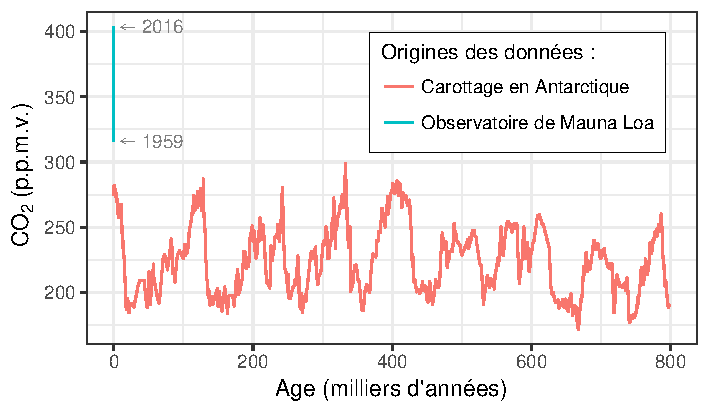
\includegraphics{figures/CO2Emissions.pdf}
	\caption[Concentration de CO\textsubscript{2} dans l'atmosphère]{Concentration de CO\textsubscript{2} dans l'atmosphère \\ Sources : \citet{Luthi2008}, donnée du Dr. Pieter Tans, NOAA/ESRL (\url{www.esrl.noaa.gov/gmd/ccgg/trends/}) du Dr. Ralph Keeling, Scripps Institution of Oceanography (\url{scrippsco2.ucsd.edu/).}}
	\label{fig:CO2Emissions}
\end{figure}

La réalité de ce réchauffement climatique est aujourd’hui «~sans équivoque~» pour la communauté scientifique des climatologues, et l'influence de l'homme sur le système climatique est «~clairement établie~» \citep{IPCC2014}.
A moins de réduire nos émissions de gaz à effet de serre, ce changement climatique va donc s’accentuer, ainsi que ses effets. Et les populations humaines seront directement concernées. La sécurité alimentaire sera menacée du fait d’impacts négatifs sur les récoltes agricoles et la pêche. L’eau sera plus rare dans les régions sèches, menant à une plus forte compétition entre les usages. Les événement extrêmes -- vagues de chaleur, précipitations violentes, cyclones --, et leurs conséquences -- inondations, sécheresses et incendies -- pourraient continuer à croitre en fréquence ou en intensité. Les océans vont continuer de s’acidifier et de se réchauffer, avec une hausse globale du niveau des mers. 
Enfin, ces bouleversements frapperont inégalement les populations : les plus démunis sont aussi les plus vulnérables aux effets des changements climatiques \citep{IPCC2014}.


\subsection{Les renouvelables, technologies clés pour l'atténuation}
Face à ces menaces, l’Accord de Paris, approuvé le 12 décembre 2015, se fixe pour objectif de «~conten[ir] l’élévation de la température moyenne de la planète nettement en dessous de 2° C par rapport aux niveaux préindustriels~». 
Dans cette optique, l’accord rappelle l’importance de cesser l’investissement dans les énergies fossiles, afin de rendre les flux financiers «~compatibles avec un profil d’évolution vers un développement à faible émission de gaz à effet de serre~». Il réaffirme également, dans l’article 4, l’objectif d’atteindre le plus rapidement possible la neutralité carbone : «~les Parties cherchent à parvenir au plafonnement mondial des émissions de gaz à effet de serre dans les meilleurs délais ».

Pour prendre la relève des énergies fossiles et atteindre le «~net zéro carbone~» permettant de plafonner les émissions, les renouvelables ont un rôle clé à jouer. Ces nouvelles technologies permettent en effet de continuer à utiliser l’énergie pour nos activités économique, tout en réduisant notre empreinte carbone.
Les énergies renouvelables ne sont pas une panacée, un remède miracle permettant d’atteindre aisément nos objectifs climatiques. Leur déploiement doit s’accompagner d’efforts sur d’autres fronts, notamment sur l’efficacité énergétique, au cœur de la stratégie de l’AIE\footnote{« \textit{there is no realistic, or affordable, energy development strategy that is not led by energy efficiency. For the IEA, it is the first fuel}~» \citep{IEA2016Efficiency}},
et la sobriété énergétique\footnote{L'association négaWatt définit la sobriété énergétique comme le fait de «~réduire à la source la quantité d’énergie nécessaire pour un même service, c’est-à-dire mieux utiliser l’énergie à qualité de vie constante~», \url{https://negawatt.org/La-demarche-negaWatt}}, concept central dans la démarche négaWatt en France\footnote{«~La sobriété et l’efficacité sont les clés de l’inflexion de la demande~»\citep{NegaWatt2017}}, et l'adaptation aux changements climatiques.
Mais ces grandes familles d’action ne sauraient être suffisantes. Même avec une diminution volontariste de la consommation comme dans le scénario négaWatt, la demande d’énergie reste conséquente. Les renouvelables sont donc un levier incontournable de l’action contre les changements climatiques.


\subsection{Deux grands enjeux}
Ma thèse s’attache à étudier deux grands enjeux autour du déploiement des renouvelables : le choix d’une stratégie de long terme, et la question des emplois liés à ces énergies renouvelables.

Le choix de stratégie de déploiement, c’est à la fois la détermination d’un niveau cible et d’une vitesse de développement. Quelle part de renouvelables veut-on dans le mix énergétique, et à quel rythme faut-il les faire entrer dans le système jusqu’à atteindre cette cible ? 
Nous présentons les enjeux de ces questions dans la section \ref{sec:intro_renouvelables}.

La thématique des emplois dits «~verts~» est extrêmement présente dans les débats publics et académiques. Mais le contenu en emploi des renouvelables est-il si élevé, comme cela est souvent avancé ? Et si investir dans les renouvelables plutôt que dans les énergies fossiles crée effectivement de l’emploi, quels sont les mécanismes économiques sous-jacents à ce bilan positif ? Nous présentons l’importance de ces questions dans la section \ref{sec:intro_emploi}.



\section{Quelle stratégie de déploiement des énergies renouvelables ? Une application au secteur électrique français}

\label{sec:intro_renouvelables}

\subsection{Les points de tension pour établir une stratégie : Inerties, arbitrages temporels et incertitudes}

\subsubsection{De profonds bouleversements}

Le déploiement rapide des renouvelables implique un remaniement profond des infrastructures énergétiques. Par exemple, dans la production d’électricité, il s’agit de passer d’un système centralisé autour de quelques centrales pilotables et un réseau fonctionnant dans une logique descendante, à un système décentralisé devant des flux variables et multidirectionnels. Il faut donc repenser non seulement les moyens de production, mais aussi tous les réseaux électriques qui les relient.
Même exemple dans les transports : sortir du tout carbone implique de repenser les technologies des véhicules, mais également toute l’infrastructure associée, avec par exemple l’installation de bornes de recharge électrique, des pompes à gaz ou des recharges à hydrogène, selon la technologie choisie du véhicule.
Ces évolutions impliquent d’importants enjeux financiers. 1,8 mille milliards sont investis chaque année dans les infrastructures énergétiques \citep{IEAWIR2016}. Pour limiter le réchauffement climatique, ces flux doivent être redirigés vers des ressources à faibles émissions. 

\subsubsection{Des arbitrages inter-temporels}
L’ampleur des bouleversements en cours et à venir, et des montants en jeu, suscite de nombreux débats. Si l’objectif de décarboner les émissions est aujourd’hui largement partagé, les stratégies pour y parvenir divergent. 

Etablir une stratégie, c’est «~coordonner des actions, de manœuvrer habilement pour atteindre un but~» selon le dictionnaire Larousse. La finalité semble ici claire : décarboner les sources d’énergie afin de limiter le réchauffement climatique. Au niveau mondial, l’objectif reste celui de contenir l’élévation de la température moyenne de la planète en dessous de 2°C par rapport aux niveaux pré-industriels. Au niveau national, depuis l’Accord de Paris, chaque pays définit ses propres engagements en termes d’émissions\footnote{Les deux objectifs n’étant pas nécessairement compatibles : les contributions volontaires cumulées aboutiraient ainsi à un réchauffement proche de 3° C}. Se pose alors la question du juste rythme, de la vitesse de cette transition, pour atteindre chaque objectif de la façon la plus «~habile~».

Un point de tension provient de l’attitude à adopter face à l’évolution du coût des énergies. Les coûts des énergies renouvelables diminuent rapidement. L’exemple le plus emblématique est celui des panneaux solaires, dont le coût a été divisé par plus de 4 en moins de sept ans \citep{Lazard2016}. Le coût des éoliennes a également été réduit, de 66\% en sept ans \citep{Lazard2016}. Le facteur quatre a également été observé pour les batteries sur la même durée \citep{McKinsey2017EV}, et est attendu pour l’éolien offshore d’ici 2020 \citep{McKinsey2017Wind}. Faut-il agir au maximum tout de suite, ou lisser l’effort dans le temps pour bénéficier des baisses de coûts ? En effet, plus l’action est progressive, et plus il est possible de bénéficier des progrès de la R\&D et des retours d’expérience, et donc de décarboner à moindre coût.
On voit ici surgir la question des arbitrages inter-temporels. Dans une perspective d’analyse coût-bénéfice, ces arbitrages doivent mettre en regard le coût des émissions supplémentaires face au bénéfice de payer moins cher des technologies qui auront bénéficié de davantage de R\&D ou de plus de retours d’expérience. Cette approche coût-bénéfice est cependant limitée, dans le cas du changement climatique, par la difficulté à évaluer les dommages climatiques. Une première raison est l’incertitude liée aux potentiels effets de seuil pour un réchauffement supérieur à 2° C par rapport à l'ère pré-industrielle. Une seconde incertitude est liée à la difficulté à évaluer le coût d’une vague de migrations climatiques, d’une vie humaine ou de la perte d’un écosystème. 
Pour toutes ces raisons, l’approche coût-bénéfice est aujourd’hui de plus en plus délaissée au profit d’une méthode dite de coût-efficacité : il s’agit d’établir la stratégie à moindre coût pour aboutir à un objectif fixé d’avance (les 2° C ou les objectifs d’un Etat). L’arbitrage intertemporel repose alors sur la notion de l’actualisation.\footnote{Le choix d’un taux d’actualisation se fonde souvent sur la règle de \citet{Ramsey1928} : $r = \delta + \gamma \cdot g$,
où $r$ est le taux d’actualisation, $\delta$est le taux de préférence pur pour le présent, $g$ est le taux de croissance du revenu individuel, et $\gamma$ est l’élasticité de l’utilité marginale de consommation. \citet{Gollier2011} recommande d’utiliser un taux de 2.5~\% à 3.5~\% pour des horizons inférieurs à 20 ans, et de 1~\% pour des termes au-delà de 100 ans. 
} 

Ainsi présenté, le problème peut paraître simple : en actualisant les prévisions des différents paramètres du problèmes (coût des technologies, demande d’énergie, etc), le choix d’une stratégie revient à un simple problème d’optimisation. 
Mais ce problème est en réalité rendu complexe par la conjonction de deux facteurs : les inerties des systèmes énergétiques, et les fortes incertitudes sur les paramètres clés de la décision.

\subsubsection{Inertie des systèmes énergétiques}
Le premier point concerne la gestion des infrastructures déjà existantes, qu’il s’agisse de moyen de production d’énergie ou de réseaux. Il faut réussir à sortir rapidement de ces énergies carbonées, tout en limitant les pertes économiques importantes qui découleraient d’actifs échoués. Il y a donc toute une dépendance au sentier à prendre en compte. Les choix passés historiques définissent les capacités et les moyens de l’action, d’autant plus que les infrastructures énergétiques s’inscrivent dans la durée. Une centrale à gaz ou à charbon peut fonctionner plus de 50 ans \citep{IEA2005}. La durée de vie des réseaux électriques est encore supérieure : les réseaux électriques français ont été installés durant le deuxième quart du XX\up{è} siècle. Ces longues durées de vie induisent une inertie du système dont doit tenir compte toute politique climatique.

\subsubsection{Incertitudes}
Cependant, ces problématiques d’inertie et d'évolution des coûts sont décuplées par la présence d’incertitudes multiples.
Une première catégorie d’incertitude provient des coûts des technologies futures. La rapide décroissance du coût des énergies renouvelables n’avait pas été anticipée par les experts \citep{Metayer2015}. Cette mauvaise anticipation du passé souligne la fragilité des estimations futures. La rapide baisse des coûts technologiques va-t-elle se poursuivre, ou ceux-ci vont-ils finir par se stabiliser ? 
Une seconde catégorie d’incertitudes concerne la croissance économique. La crise économique de 2008 et la grande dépression qui s’ensuivit nous rappellent avec force la possibilité d'imprévus de grande ampleur. Or, l’évolution de cette croissance est importante à double titre : par son impact sur la demande d’énergie, et par son rôle dans l’estimation du taux d’actualisation. 
Une troisième catégorie a trait aux coûts des énergies fossiles. Les rapports alarmants sur le risque d’un pic de pétrole ne manquent pas depuis le célèbre rapport du Club de Rome, \textit{The limit to growth} \citep{Meadows1972}. En 2012, les prix du Brent dépassèrent les 130 \$ par baril, ravivant des inquiétudes sur l’imminence du pic. Mais l’avènement de la fracturation hydraulique et l’arrivée massive sur le marché mondial du pétrole de schiste américain a fait replonger les prix à des niveaux historiquement bas en 2015. Alors que les prix s’établissaient autour de 110 \$ par baril entre 2011 et 2014, ils se sont effondrés aux alentours de 50 \$ après 2015. Autant de rebondissements révélateurs de l’incertitude sur les ressources, les techniques d’extraction et, \textit{in fine}, les prix. 
Des incertitudes techniques similaires existent pour le gaz, comme en témoigne la révolution des gaz de schiste. En outre, le prix du gaz est en partie indexé sur celui du pétrole en Europe, et subit donc ses fluctuations. 

Enfin, il existe une incertitude sur la volonté politique de prendre en compte le changement climatique. Très concrètement, pour l’économiste, cette incertitude prend notamment la forme d’une incertitude sur le prix du CO\textsubscript{2} à considérer. Le marché de quotas européen, le SCEQE -- plus connu sous l’acronyme anglais de EU ETS -- considéré comme un exemple emblématique d’un marché de quotas, a ainsi connu de fortes variations. Le prix a atteint 30 euros la tonne en 2008, mais est depuis redescendu aux alentours de 5 euros par tonne \citep{Marcu2016}.

Notons bien qu’il s’agit ici d’incertitudes radicales. Ce concept d’incertitude, au sens de \citet{Knight1921}, est à distinguer de celui de risque par l’impossibilité même de prévoir une distribution de probabilité des cas possibles \footnote{On peut trouver dans la littérature d’autres terminologies équivalentes, et notamment celle d'incertitude profonde (\textit{deep uncertainty}).} :
\begin{quote}
	«~La différence pratique entre les deux catégories, le risque et l’incertitude, est que, s’agissant de la première, la distribution du résultat parmi un ensemble de cas est connue (soit par le calcul a priori, soit par des statistiques fondées sur les fréquences observées), tandis que ceci n’est pas vrai de l’incertitude en raison de l’impossibilité de regrouper les cas, parce que la situation à traiter présente un degré élevé de singularité~»\citep[p. 233]{Knight1921}.
\end{quote}
Il est bien sûr impossible de pouvoir définir avec certitude une distribution de probabilité sur les coûts futurs de renouvelables, le taux de croissance économique, le prix des ressources fossiles ou encore celui du CO\textsubscript{2}. Nous sommes donc bien dans le cas de l’incertitude radicale. Quelle valeur prendre pour chaque paramètre incertain ? Prendre une unique valeur pour chaque paramètre incertain pour minimiser les coûts reviendrait en quelques sortes à nier l’incertitude. Nous cherchons donc une approche qui prenne à bras-le-corps ces incertitudes, qui les intègre pleinement au problème, sans les réduire artificiellement. Comme l’a noté Edgar Morin dans \textit{la Méthode}, “La connaissance progresse en intégrant en elle l'incertitude, non en l'exorcisant” \citep{Morin2008}.
En outre, on voit que face à cette incertitude radicale, différentes options politiques peuvent être également défendables, selon les choix d’un politique, selon ses convictions intimes, ou pour le dire autrement, selon ses probabilités implicites sur les futurs états du monde. Par exemple, un décidant convaincu que les prix du pétrole vont remonter rapidement voudra accélérer la décarbonation des transports. Et il n’est pas possible de dire qu’il a évidemment tort de faire cette hypothèse – non plus qu’il a évidemment raison. Nous cherchons donc une approche qui ne propose pas nécessairement une unique solution.

Toutes ces incertitudes se combinent avec les questions d’inertie, et cette conjonction rend le problème d’arbitrage inter-temporel extrêmement complexe. L’inertie implique d’anticiper l’impact des choix faits, car ceux-ci nous engagent sur plusieurs décennies ; mais l’incertitude empêche d’anticiper parfaitement. Comment, dès lors, déterminer la meilleure stratégie ? Nous tentons de répondre à cette question en nous intéressant plus spécifiquement au cas du déploiement des renouvelables en France.

\subsection{Une application au secteur électrique français}

\subsubsection{De l’importance du secteur électrique dans la transition}
Dans ma thèse, j’ai choisi d’étudier la question des inerties et des incertitudes à travers le cas du secteur électrique français. Le secteur électrique est au cœur de la transition énergétique. Il s’agit en effet d’un secteur contribuant largement aux émissions mondiales, tout en présentant des possibilités techniques de substitutions : les centrales à gaz, à charbon et à fuel peuvent être remplacées par des éoliennes, des panneaux solaires ou du biogaz.

La révolution des énergies renouvelables électriques a d’ailleurs déjà commencé. L’année 2015 fut celle d’un record absolu en termes de capacités renouvelables installées au niveau mondial avec 153 GW \citep{InternationalEnergyAgency2016}. L’investissement dans les renouvelables électriques a également atteint un nouveau record, en dépit de la plongée des prix du pétrole : 265,8 milliards de dollars, soit plus du double des investissements dans les centrales à gaz ou à charbon [REN21, Global status report 2016]. 
Si la Chine est passée en tête en termes de capacité installée, l’Europe n’est pas en reste. En termes de production renouvelable électrique par habitant (hors hydraulique), les cinq premiers pays du G20 sont tous européens : Danemark, Allemagne, Suède, Espagne et Portugal \citep[p. 21]{REN212016}. Le Danemark en particulier s’est fixé l’objectif de se passer des énergies fossiles à l’horizon 2050\footnote{\url{http://denmark.dk/en/green-living/strategies-and-policies/independent-from-fossil-fuels-by-2050/}}, et en 2015, la production des renouvelables représentaient déjà 56~\% de la consommation d'électricité dans le pays\footnote{\url{https://ens.dk/en/press\#/pressreleases/renewables-now-cover-56-procent-of-electricity-consumption-1672848}}. 

\begin{figure}[!ht]
	\centering
	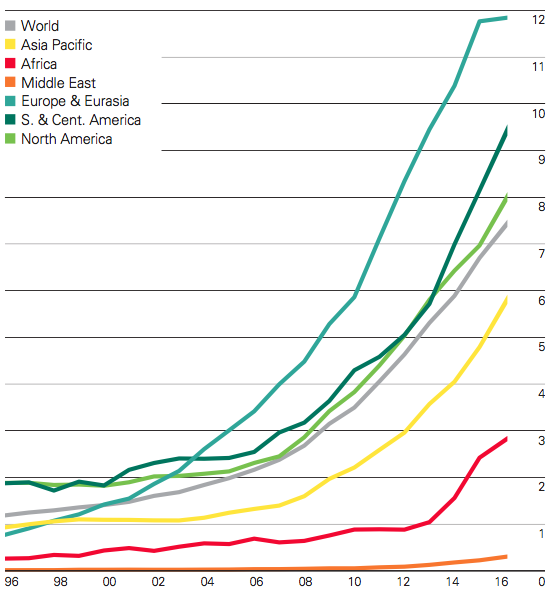
\includegraphics[height=7cm]{figures/BP_ENR_Expansion.png}
	\caption[Expansion of renewable energies in the power sector]{Expansion of renewable energies in the power sector.\\Source: \citet[p. 43]{BP2017}}
\end{figure}

Cette révolution est portée par une volonté politique, avec la mise en place de mécanismes de soutien volontaristes par certains Etats : tarifs d’achat garantis, obligation de quotas, exemption de taxes, appels d’offres, aides à l’investissements, etc.\citep{EuropeanCommission2013}. Et elle est facilitée par une décroissance rapide des coûts des renouvelables. On a ainsi vu s’amorcer une boucle vertueuse, où le soutien politique accélère la diminution les coûts, ce qui facilite le soutien politique en retour.

\subsubsection{Contexte politique français}
En France, le mix électrique est déjà largement décarboné du fait de la grande part du nucléaire, qui représentait 72~\% de la production d’électricité en 2016. Avec l’hydraulique à 12~\%, ceci ne laisse qu’une part marginale aux nouvelles énergies renouvelables. L’éolien et le solaire ne comptaient ainsi que pour 5,5~\% de l'électricité produite en 2016 \citet{RTE2016}. 
Mais la question du déploiement des renouvelables est sur la table. Avec la Loi sur la Transition Energétique pour la Croissance Verte (LTECV), la France s’est engagée à porter à 40~\% de la production d’électricité la part des renouvelables d’ici à 2030, et à réduire la part du nucléaire à 50~\% d’ici 2050. Certains doutes existent quant au fait que la France atteigne effectivement ces objectifs, notamment du fait des difficiles compatibilités entre les différents objectifs mentionnés dans la loi - l’IDDRI parle de «~quadrature du cercle~» \citep{Rudinger2017}. Le débat reste donc ouvert.

\begin{figure}[!ht]
	\centering
	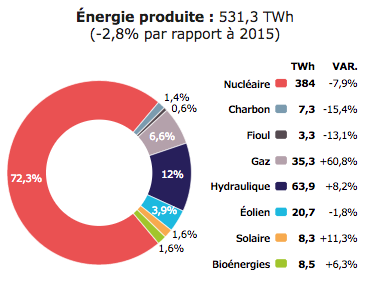
\includegraphics[width=7cm]{figures/RTE_Mix.png}
	\caption[Mix électrique français en 2016]{Mix électrique français en 2016.\\Source: \citet[p. 4]{RTE2016}}
\end{figure}

La situation du parc électrique français présente donc toutes les caractéristiques qui rendent le choix d’une stratégie difficile : la nécessité de faire des choix inter-temporels, en présence d’incertitudes et d’inerties. Inerties et incertitudes sont même particulièrement prégnantes ici avec la technologie nucléaire, au cœur du débat français sur la transition. 

Ce débat a été particulièrement visible lors de la campagne présidentielle de 2017. Une étude diffusée le 13 mars par l’Institut Montaigne présente le nucléaire comme la seule option «~rationnelle~», et évalue à 217 milliards d’ici 2035 le coût d’une sortie de l’atome.\footnote{\url{http://www.institutmontaigne.org/presidentielle-2017/propositions/benoit-hamon-climat-environnement-et-agriculture-sortir-progressivement-du-nucleaire}} Quatre jours plus tard, une réponse publiée sur le site «~Décrypter l’énergie~» estime au contraire que la sortie du nucléaire représenterait un bénéfice de 24 milliards.\footnote{\url{http://decrypterlenergie.org/fermeture-du-parc-nucleaire-un-cout-largement-surestime-par-linstitut-montaigne}} Le grand écart dans cette bataille de chiffres est surtout révélateur des incertitudes considérables qui entourent la filière. C’est seulement en prenant pleinement acte des nombreuses inconnues qu’il sera possible de faire progresser le dialogue et d’établir une feuille de route pour l’industrie nucléaire française.
Rappelons que l’année a été riche en rebondissements pour la filière nucléaire. Après le démantèlement d’Areva, fortement endettée, un audit interne à l’entreprise a mis à jour deux anomalies génériques. La première concerne des irrégularités qui «~s'apparentent à des falsifications~»\footnote{Selon les propres termes de Pierre-Franck Chevet, président de l'ASN, \url{http://abonnes.lemonde.fr/entreprises/article/2015/07/07/areva-connaissait-de-longue-date-les-anomalies-de-la-cuve-de-l-epr_4674521_1656994.html}} constatées dans plus de 400 dossiers de fabrication de composants. La seconde a trait à des inquiétudes sur la résistance des cuves – élément central et impossible à remplacer - des réacteurs en fonctionnement. Plusieurs centrales nucléaires ont été arrêtées pour inspection cet hiver, allant jusqu’à faire craindre un possible black-out du système électrique français. Ces anomalies ont touché jusqu’à la cuve de l’EPR de Flamanville, faisant craindre de nouveaux reports pour un chantier qui devait initialement s’achever en 2012, mais ne cesse d’accumuler les retards et les surcoûts. Tous ces éléments ne peuvent que raviver la controverse sur les risques et les coûts réels de cette énergie. 
Or, les centrales nucléaires françaises atteignent aujourd’hui 40 ans, leur durée de vie initialement prévue. La question du futur de l’atome est donc à nouveau sur la table, après quarante ans d’une histoire héritée du premier choc pétrolier. EDF estime pouvoir rénover les réacteurs actuels afin de les prolonger jusqu’à 60 ans, grâce à une opération dite de «~Grand Carénage~» estimée à 100 milliards d’euros. Faut-il rénover ces centrales ? Ou plutôt, combien de centrales faut-il rénover, et lesquelles ?

\subsection{Méthodologie : Décision robuste et modèle d’optimisation du parc électrique}

\subsubsection{Déterminer des stratégies robustes}

Face à ces incertitudes, l’approche traditionnelle des économistes modélisateurs consiste à choisir a priori un jeu de paramètres pour trouver un optimum, puis à procéder à des tests de sensibilité en faisant varier les paramètres de départ sur les plages plausibles de valeurs. Si le résultat s’avère insensible, autrement dit si l’optimum reste invariant pour toutes les valeurs plausibles de paramètres, on peut alors conclure que l’on a trouvé un unique optimum.
Mais que faire si les résultats varient avec différentes valeurs plausibles de paramètres ? 

Une solution de continuité consisterait à donner la solution optimale correspondant à chaque jeu de paramètre. On aboutirait à plusieurs solutions possibles, selon l'état du futur anticipé. Mais cette approche peut se révéler paralysante pour le décideur, puisqu'elle aboutit à une multiplicité de résultats, sans permettre de choisir finalement une solution.

Face à ces incertitudes radicales, réduire de façon artificielle les incertitudes sur les paramètres, de façon à retrouver un unique optimum, n’est pas une option. Il faut une approche qui admette la possibilité d’aboutir à plusieurs options possibles, à plusieurs stratégies plausibles pour certaines valeurs des paramètres. Cette pluralité de solutions peut permettre de faire le lien avec le débat public : souvent, en présence de fortes incertitudes, plusieurs solutions sont proposées sans qu’il soit possible de déterminer la meilleure avec une absolue certitude. 

L’enjeu est alors celui d’une aide à la décision. Il s’agit de simplifier la tâche du décideur face à la multiplicité des paramètres d’entrée du problème. Quels sont les paramètres ou combinaisons de paramètres qui s’avèrent décisifs ? Nous chercherons à réduire un problème comportant initialement n paramètres, pour aboutir proposer deux ou trois ensembles de paramètres. Le décideur n’aura alors plus qu’à choisir entre ces ensembles. Mais au final, ce choix nécessite que le décideur fasse un pari sur l’avenir, d’où le choix du titre de l’article qui fait la première partie de cette thèse : le pari nucléaire français (\textit{the French nuclear bet}).

Il peut être également intéressant de délaisser la notion paralysante d’optimum, au profit du concept de trajectoire robuste, défini par \citet{Lempert2006} comme «~une stratégie qui offre une performance satisfaisante dans un grand nombre de futurs plausibles~» - un futur, ou futur état du monde, correspondant à un jeu de paramètres pour notre modèle.
Cette définition générale doit cependant être adaptée à notre objet d’étude particulier : quel indicateur choisir pour la performance, et qu’est-ce qu’un niveau satisfaisant ?
Pour notre analyse le parc électrique français, nous cherchons assez classiquement à minimiser l'ensemble des coûts, en incluant les coûts en investissement dans la construction du moyen de production, le coût variable de son opération et de sa maintenance, mais aussi les coûts liés au prix du CO\textsubscript{2}. Ce coût total sera donc l’indicateur de performance d’une stratégie.
Une stratégie sera jugée satisfaisante si son coût est assez proche de l’optimum pour le même jeu de paramètres. En utilisant la terminologie de \citet{Savage1950}, on peut introduire le terme de regret, c’est-à-dire de l’écart à l’optimum. Au final, une stratégie robuste est donc celle qui offre un faible regret pour un grand nombre de futurs plausibles.

Pour satisfaire ce cahier des charges que j’ai ainsi dessiné, la méthodologie qui m’a paru la plus appropriée est celle présentée par \citet{Lempert2006}, qu’ils appellent la fabrique de décision robuste (\textit{Robust Decision Making en anglais}, RDM). Cette méthode consiste à appliquer des analyses statistiques sur les résultats d’un grand nombre de scénarios, en mobilisant la notion de regret. Elle s’est initialement développée autour de la thématique du changement climatique, grâce à l’essor des capacités de calculs informatiques. Mais elle peut également être appliquée à une grande variété de cas d’étude : la gestion de l’eau des rivières, l’énergie, la résilience des côtes au changement climatique, etc.\footnote{Une grande liste de projets est visible sur le site \url{https://www.rand.org/topics/robust-decision-making.html?content-type=brief}} Je présente cette méthode plus en détail dans le chapitre \ref{chap:nuclear_bet}.
	
\subsubsection{Cahier des charges pour le modèle d’optimisation}

\textbf{De la nécessité d’aller au-delà du LCOE}

Une métrique est très largement utilisée dans le secteur de l’électricité pour mesurer la compétitivité de différents moyens de production : le coût moyen actualisé de l’électricité, ou plus communément appelée LCOE (\textit{Levelized Cost of Electricity}).
Cet indicateur rassemble en un chiffre unique tous les coûts sur l’ensemble du cycle de vie de la centrale : coûts d’investissement, d’opérations et maintenance, coût du combustible, du financement, du démantèlement, et il les rapporte à la quantité totale d’électricité produite. Le LCOE correspond donc au coût moyen pour produire un mégawattheure d’électricité avec un certain moyen de production.

De façon plus formelle, l'\citet{InternationalEnergyAgency2015} définit le LCOE de la façon suivante :
$$LCOE = \frac{\sum_t (Capital_t + O\&M_t + Fuel_t + Carbon_t + D_t) / (1+r)^t}{\sum_t MWh / (1+r)^t}$$
où
\begin{itemize}
	\item MWh = le montant d'électricité produite en MWh, supposé constant ;
	\item $(1+r)^t$ = le facteur d'actualisation;
	\item $Capital_t$ = Ensemble des coûts de capital pour la construction à l'année $t$;
	\item $O\&M_t$ = Coûts d'opération et Maintenance à l'année $t$;
	\item $Fuel_t$ = Coûts de combustible à l'année $t$;
	\item $Carbon_t$ = Prix du carbone à l'année $t$;
	\item $F_t$ = Coûts de démantèlement et gestion des déchets à l'année $t$.
\end{itemize}

Cette métrique est utile pour comparer des moyens de productions pilotables. Mais elle n’est plus adaptée pour des moyens de productions variables et non pilotables, comme les énergies éoliennes et solaires. Dès 2011, \citet{Joskow2011a} la dénonçait comme une «~métrique biasée~» (\textit{flawed metric}). En effet, elle suppose que l’électricité est un produit homogène, et donc régi par la loi d’un prix unique. Mais cette hypothèse est erronée, car elle ignore la variabilité temporelle de la production. Or, la valeur d’un mégawattheure varie selon l’heure du jour et selon la saison : elle est très élevée pendant les heures de pointes, et faible pendant les creux, notamment la nuit. Comme l’électricité ne peut être stockée, il y a bien une hétérogénéité du bien électricité. L’approche par le coût du LCOE ne mesure pas la valeur pour le système, qui est pourtant le bon indicateur : si je produis de l’électricité à faible coût, mais à un moment où personne n’en demande, ma production n’a aucune valeur !

Cette variation temporelle de la valeur de l'électricité est renforcée par les phénomènes d’autocorrélation de la production des renouvelables variables. Les panneaux solaires produisent tous à leur maximum vers midi. Ainsi, plus le nombre de panneaux solaires est élevé, plus le prix de l’électricité (représentatif de sa valeur à chaque instant) sera faible à midi. La situation est similaire avec les éoliennes : plus le taux de pénétration des renouvelables est important, plus le prix de marché au moment de leur production diminue, d’où une compétitivité décroissante des renouvelables variables avec le taux de pénétration \citep{Hirth2013}.

\citet{Hirth2016} distinguent par ailleurs deux autres facteurs d’hétérogénéité : le lieu de la production, ce qui inclut notamment la distance au lieu de consommation, et le délai entre le moment du contrat et celui de la livraison. Au total, ces trois sources d’hétérogénéité influent sur la valeur de la production pour le système, ce qui n’est pas inclus dans la notion de LCOE, qui ne traite que des coûts. 
Ces limitations du LCOE justifient l’utilisation d’un modèle intégré du système électrique.

\vspace{1em}
\textbf{Quel modèle choisir ?}

Une grande variété de modèles existe pour l’analyse du mix électrique. Le choix d’un modèle ne peut se faire qu’à travers une analyse précise des besoins liés à la question de recherche.
On peut déjà identifier quelques prérequis :
\begin{itemize}
	\item Je souhaite étudier l’investissement à long terme. Il faut donc que l’investissement soit inclus comme variable endogène au problème. \citet{Petitet2016} distingue trois grandes catégories de modèles : les modèles d’optimisation inter-temporels, les modèles à agents hétérogènes avec des approches par les systèmes dynamiques ; et enfin les modèles micro-économiques de type Bertrand, Cournot ou Stackelberg pour analyser les pouvoirs de marché. 
	\item Je m’intéresse au cas de la France, marché libéralisé mais sous un contrôle strict de la Commission Européenne, et notamment des règles anti-concurrence. En France, c’est plus particulièrement la Commission de Régulation de l’Energie (CRE) qui est en charge de cette mission de surveillance pour le compte de l'Autorité de la Concurrence. Je ne m’intéresse donc pas à aux modèles de concurrence imparfaite et aux pouvoirs de marché. Je me place au contraire dans un cadre de concurrence parfaite, c’est-à-dire que tous les acteurs économiques prennent le prix du marché comme une donnée externe dans leurs décisions, ils ne peuvent l’influer. 
	\item Je cherche à établir ce qui pourrait être la meilleure stratégie plus qu’à anticiper ce que sera l’évolution. Je m’inscris donc dans une perspective plus normative que positive. Les modèles à optimisation inter-temporelle me paraissent être plus à même de remplir ce rôle que les approches en simulation. C’est donc sur cette famille de modèles que j’ai arrêté mon choix.
\end{itemize}

\textbf{Hypothèses structurantes}

Dans notre modèle, nous maximisons le profit des producteurs. En effet, d’après le premier théorème du bien-être, cette maximisation conduit à un optimum de Pareto – à condition que les marchés soient complets (sans coût de transaction et avec une information parfaite des agents) et que les firmes soient preneuses de prix. Puisqu’on se place dans une démarche normative, nous supposerons ces deux conditions. 
Nous supposons en outre une parfaite compétition entre les agents économiques, et une demande d’électricité exogène. Cette dernière hypothèse implique notamment que je ne modélise pas explicitement l'élasticité de la demande, ni à court terme ni à long terme. La littérature empirique donne des résultats variables pour les valeurs de ces élasticités. Pour donner un ordre de grandeur, une méta-analyse de \citet{Labandeira2016} les évalue à 0.23 et 0.67 respectivement. Idéalement, il faudrait aussi détailler les différences entre ménages, industries électro-intensives et autres industries, voire même les différences saisonnières dans ces élasticités \citep{Fan2011}. Mais dans tous les cas, il est difficile de prévoir quelle seront ces élasticités dans les années et décennies à venir. Par exemple, le déploiement des compteurs intelligents Linky en France pourrait permettre de jouer davantage sur la demande d'électricité pour apporter de la flexibilité, avec la possibilité de faire passer plus de consommateurs vers une tarification en temps réel et le déploiement d'appareils ménagers réactifs aux prix.
En pratique, l'approximation de demande exogène me semble raisonnable pour un gain très important en termes de temps de calcul. Il s'agit d'ailleurs d'un choix très largement partagé dans la communauté des modélisateurs. D’un point de vue théorique, cette hypothèse permet de poser une équivalence duale entre la maximisation du profit et la minimisation des coûts. 
On ramène donc le problème à celui d’une minimisation des coûts, en sachant que – sous les hypothèses mentionnées – cet objectif est équivalent à maximiser l’utilité.

L’étape suivante consiste à définir les phénomènes que l’on souhaite représenter. Pour notre question de trajectoire optimale, les points suivants m’ont paru essentiels :
\begin{itemize}
	\item Représenter l’ensemble de la trajectoire, de façon continue et cohérente. Il faut une représentation fine des durées de vie des centrales nucléaire, et des prolongations permises par une rénovation.
	\item Représenter l’hydraulique de façon fine, avec notamment un fonctionnement des barrages et des stations de pompage endogène, qui s’adapte au déploiement des renouvelables. La France possède un parc hydraulique qui peut faciliter le déploiement des énergies renouvelables. En effet, la flexibilité de l’hydraulique améliore la valeur des énergies renouvelables variables pour le système électrique \citep{Hirth2016a}.
	\item Avoir une représentation temporelle suffisamment fine pour représenter les variations horaires (avec les pics de demande le matin et le soir), hebdomadaires (avec les baisse de demande le week-end) et saisonnières (avec une production éolienne plus importante en hiver, une production solaire plus forte en été, et une demande d’électricité plus forte en hiver).
\end{itemize}

Pour répondre à tous ces objectifs, j’ai choisi de construire mon propre modèle d’optimisation du parc électrique, que j’ai appelé FLORE (French Linear Optimization for Renewable Expansion). Ce modèle est présenté plus en détail dans le chapitre \ref{chap:nuclear_bet}.
Toutes les équations et données du modèle sont disponibles en ligne, dans un esprit de transparence et de partage nécessaire pour la reproductibilité des résultats et d’efficacité du travail de recherche. Je m’inscris pleinement dans cette démarche, recommandée par \citet{Pfenninger2017} et encore trop absente dans le domaine de l’économie de l’énergie.
Dans le chapitre \ref{chap:nuclear_bet}, je combine la méthodologie RDM et le modèle FLORE afin d’étudier les stratégies robustes de déploiement des renouvelables électriques en France.

\section{L’impact de la transition énergétique sur l’emploi}
\label{sec:intro_emploi}


\subsection{L'importance politique et sociale de l'emploi}

\subsubsection{L'emploi, argument moteur des décisions publiques}

L’emploi est aujourd'hui un argument déterminant pour initier une action politique.
En France, le taux de chômage en France est passé de 7,3~\% en avril 2008 à plus de 10~\% depuis octobre 2012 \citep{Eurostat}. Chez les jeunes, ce taux monte même à 24~\% \citep{OCDE} faisant craindre une génération perdue.
De fait, le chômage est de loin la première préoccupation des français, en 2012 \citep{TNSSOFRES2012} comme en 2017 \citep{IFOP2017}.
L'importance politique de cette thématique s'est retrouvée dans la promesse faite par le Président François Hollande d'inverser la courbe du chômage -- engagement ensuite transformé en un leitmotiv politique qui traversa tout le quinquennat : «~Toutes nos forces seront tendues vers un seul but : inverser la courbe du chômage~», déclare-t-il ainsi dans ses premiers v\oe{}ux télévisés en 2013.

Cette prépondérance de l'emploi se retrouve dans les débats sur la transition énergétique. Bien plus qu’un épiphénomène ou qu’un simple co-bénéfice, l’emploi est un argument majeur. Il semble même presque parfois qu’un renversement s’opère au niveau politique : la transition énergétique ne serait finalement que le co-bénéfice d’une politique qui vise avant tout à réduire le chômage. Ainsi, en France, deux ans de débats sur la politique énergie-climat ont abouti à une loi intitulée : «~Loi de Transition Energétique \textit{pour} la croissance verte~»\footnote{Loi n° 2015-992 du 17 août 2015. L'italique est de mon fait.
}. La préposition \textit{pour} indique clairement que la finalité première est bien la croissance. L'écologie n'est représenté par un qualificatif flou : \textit{vert}, et la transition énergétique n'est qu'un moyen pour parvenir à cette croissance. 
Sur son site web, le site du Ministère de l'Ecologie met également en avant que cette loi permettrait de générer «~100 000 emplois~». Le bénéfice en termes d'emploi est d'ailleurs présenté avant celui en termes de PIB.\footnote{On trouve les annonces suivantes sur le site du Ministère : «~La loi de transition énergétique pour la croissance verte (LTECV) favorise une croissance économique durable et la création d'emploi pérennes et non délocalisables :
\begin{itemize}
	\item elle permet la création de 100 000 emplois à court terme (dont 75 000 dans le secteur de la rénovation énergétique et près de 30 000 dans le secteur des énergies renouvelables) et de plus de 200 000 emplois à l’horizon 2030 ;
	\item le PIB devrait profiter des efforts réalisés à hauteur de 0,8~\% en 2020 et 1,5~\% en 2030.~»
\end{itemize}
\url{https://www.ecologique-solidaire.gouv.fr/loi-transition-energetique-croissance-verte}, accédé le 4 juillet 2017
}

Souligner les effets positifs en termes d’emploi est d’autant plus important que le réchauffement climatique est un exemple typique du phénomène de tragédie des communs \citep{Hardin1968}. Les biens communs sont, selon la terminologie de \citet{Samuelson1954}, des biens non-exclusifs (tout le monde peut y avoir accès a priori) mais rivaux (son usage par un individu empêche son usage par un autre). Un exemple intuitif est celui des ressources halieutiques dans les eaux internationales : tout le monde peut pêcher le poisson présent, mais une fois pêché, les poissons ne sont plus disponibles pour les autres.
Le problème est formellement identique pour les émissions de gaz à effet de serre, ou plus précisément pour la capacité d'absorption de ces gaz par la biosphère : chaque pays peut émettre ces gaz, mais la planète ne peut absorber les émissions de tout le monde à leur niveau actuel.
Comme pour la pêche, chaque Etat a intérêt à jouer les passagers clandestins et à laisser les autres faire le maximum d’efforts de réduction d'émissions. On retrouve formellement le problème du dilemme du prisonnier.

S’il était possible de montrer que la transition énergétique permet de générer des bénéfices locaux ou nationaux en termes d'emploi, il serait alors possible de sortir de ce dilemme, de dépasser la vision opposant économie et environnement. Le climat serait alors perçu comme une véritable panacée, guérissant à la fois du chômage et des réchauffement climatiques. Le support public et politique serait plus fort, accélérant la réduction de nos émissions.

\subsubsection{Importance sociale et impact sur le bien-être}

Une seconde raison pour étudier l'emploi est son importance en termes de bien-être.
La littérature sur les déterminants du bonheur souligne l’importance du facteur emploi : il existe un large fossé de bien-être subjectif entre ceux qui possèdent un emploi et ceux qui en cherchent sans succès. Comme le souligne le rapport Stiglitz : 
\begin{quote}
	«~Toutes les recherches sur le bien-être subjectif se rejoignent sur un aspect : le coût humain élevé engendré par le chômage. Les chômeurs se disent moins satisfaits de leur vie que les personnes ayant un emploi, \textit{même si l'on élimine l'effet de la baisse de revenu}~» \citep[p. 166, l'emphase est de mon fait]{Stiglitz2009}.
\end{quote}			
La question n'est pas donc celle du salaire ou du niveau de revenu. Le fait d'avoir un emploi semble intrinsèquement lié à un niveau de bonheur plus élevé. Il s'agit d'un indicateur représentant une valeur pour les individus.

Cette importance de l’emploi sur le bien-être est une d'ailleurs conclusion stable à travers les générations. C'est par exemple la conclusion des travaux de \citet{Clark2009}, qui étudie des données répétées en coupe :
«~not having a job when you want one is a major source of low well-being. [...] job values have remained fairly stable over time~». Enfin, la valeur de l'emploi est confirmée en creux est par une série de symptômes cliniques corrélés à son absence : être au chômage augmente les risques de mortalité et de morbidité, ainsi que les taux de suicide et les maladies mortelles \citep{Gerdtham2003}.


\subsubsection{La renaissance du double dividende emploi}

Moteur de l'action politique et déterminant du bien-être : on comprend bien alors l’intérêt des chercheurs pour la thématique de l'emploi. 

La branche de la littérature liée à ce sujet s'articule autour de la question du double dividende : dans quelle mesure est-il possible d'avoir une action positive à la fois pour l'économie et pour l'environnement ?
Si la métrique économique observée est plus particulièrement l'emploi, on parlera alors de double dividende emploi.

La question du double dividende emploi est apparue dans la littérature avec la prise de conscience du changement climatique. Le terme de double dividende a ainsi été introduit par Pearce en 1991 \citep{Pearce1991}.
Mais avec la Grande Récession que nous connaissons depuis la crise de 2007, la conjugaison des thématiques énergie et emploi est de plus en plus fréquente dans le domaine académique. On peut le mesurer grâce à la base de données Web of Science, qui agrège les publications de recherche. Une recherche «~employment AND energy~»\footnote{Recherche effectuée le 12 juillet 2017. Requête exacte : TS=(employment AND energy) AND SU=("Business \& Economics" OR "Environmental Sciences \& Ecology" OR "Energy \& Fuels")} donne une tendance exponentielle du nombre de travaux sur croisant ces deux sujets depuis la crise économique (cf. graphique \ref{fig:webofScience}).

Cet intérêt dépasse d'ailleurs la sphère académique, et se retrouve également dans le domaine public. En interrogeant la base de données Factiva\footnote{Recherche effectuée le 12 juillet 2017. Requête exacte : "emploi AND énergie"}, qui répertorie les parutions dans la presse française, on peut constater une forte augmentation, commençant un peu plus tôt, dès 2002, avec un pic probablement lié au débat sur la loi de transition énergétique en 2014 (cf. graphique \ref{fig:Factiva}). 


\begin{figure}[h!]
	\centering
	\subfloat[Web of Science, résultats pour "employment AND energy"] {
		\makebox[5.5cm][c]{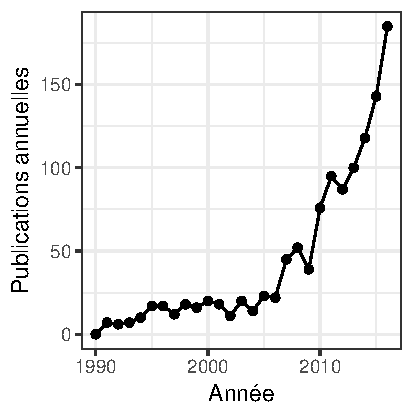
\includegraphics[height=5cm]{figures/EmploymentEnergy.pdf}}
		\label{fig:webofScience}
	} \qquad
	\subfloat[Factiva, résultats pour "emploi AND énergie"][Factiva, résultats pour \\ "emploi AND énergie"]{
		\makebox[6cm][c]{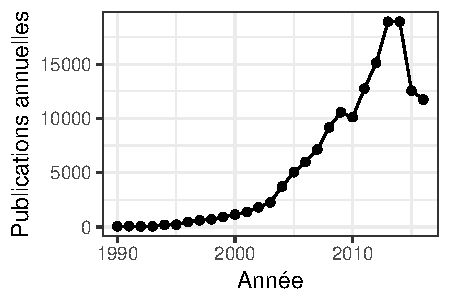
\includegraphics[height=5cm]{figures/Factiva.pdf}}
		\label{fig:Factiva}
	}
\end{figure}

C’est pour ces deux raisons, l’importance sociale de l’emploi et son potentiel de levier d’action dans la transition énergétique, que j’ai choisi l’emploi dans la transition énergétique comme deuxième thématique de ma thèse.
Plus précisément, ma réflexion a principalement porté sur deux sujets : le contenu en emploi des secteurs bas-carbone et sur les mécanismes économiques à l'origine de la création d'emploi. 
Les deux parties suivantes introduisent de façon plus détaillée les enjeux pour chacun de ces sujets.


\subsection{Le contenu en emploi des énergies renouvelables}

\subsubsection{Un concept mal défini}
L’avantage des renouvelables en termes d’emploi est souvent présenté comme découlant d'une raison très simple : les renouvelables auraient un contenu en emploi plus élevé. Par exemple, selon le réseau Sortir du Nucléaire, «~les renouvelables créent quinze fois plus d’emplois que le nucléaire~» \citep{Les7ventsduCotentin2009}. Greenpeace met en avant que cet avantage est dû au fait qu’il s’agit d’emploi «~de proximité~», «~non délocalisables~» \citep{Greenpeace2011}. Favoriser l’essor des renouvelables au détriment des énergies fossiles ou fissiles permettrait donc de générer de nombreux emplois.

Si certains secteurs ont un contenu en emploi plus élevé, alors il serait possible de créer des emplois en réallouant la demande finale vers ceux-ci. Puisqu’il s’agit simplement de réallouer, et non d’augmenter les dépenses, cette mesure peut être particulièrement attractive pour des décideurs au budget contraint. Le contenu en emploi permet d'établir une mesure du bilan net de cette réallocation. Mais il reste muet sur les mécanismes économiques sous-jacents. 

Mais la simplicité de ce message à vocation politique cache une complexité d’un autre ordre pour l’économiste. 
%cf études sur le nucléaire ?
La première concerne la définition même de contenu en emploi. Il existe en effet un flou important quant à l’unité de mesure : s’agit-il du nombre d’emploi par unité de puissance installée (kW) ? par unité d’énergie produite (kWh) ? par euro investi ou dépensé ? En pratique, ces différentes métriques coexistent dans la littérature académique : \citet{Cameron2015} observent des données en emploi par capacité installée, \citet{Quirion2013} des emplois par euro dépensé, \citet{Wei2010} par unité d’énergie produite. Mais elles sont-elles équivalentes en termes de résultats ? Quelle serait la meilleure métrique ?
Une seconde difficulté provient de l’articulation de cette notion avec d’autres éléments du débat public. L’accent est parfois mis sur le fait que les renouvelables ont un caractère local, qu’ils permettent de réduire les importations de gaz ou de charbon. Ils sont également présentés comme étant intensifs en travail, plutôt qu’en capital. Quels liens établir entre ces arguments et la notion de contenu en emploi ?
Enfin, il faut distinguer les contenus bruts en emploi et les contenus nets en emploi. Les deux sont utiles à l'analyse : le brut pour les enjeux locaux, le net pour une échelle nationale. Nous nous intéressons ici à l’effet net sur l’emploi. Or, l'éolien et le solaire ont commencé à se développer avant d’être compétitifs, grâce à des subventions. Mais ces subventions doivent être financées, \textit{in fine} au moyen d’autres taxes générant potentiellement des réduction d’emplois dans d’autres secteurs. Comment prendre en compte ces effets indirects des subventions dans la mesure du contenu en emploi, afin de mesurer un impact net ?

\subsubsection{Décomposer le contenu en emploi}

Ces interrogations m’ont amené à vouloir décomposer le contenu en emploi. Pourquoi ce contenu en emploi est-il plus élevé dans certaines branches ? Est-ce du fait d’importations plus faibles, d’une plus grande part du travail dans la valeur ajoutée, ou d’autres facteurs ? Quels sont les facteurs prépondérants expliquant les divergences d’une branche à l’autre ?
Ces questions impliquent de pouvoir décomposer le contenu en emploi, afin d'en faire ressortir les facteurs prépondérants.

Mais à travers ce travail descriptif et explicatif, nous espérons pouvoir obtenir une connaissance permettant l’action. Les conséquences sont en effet très différentes si le contenu en emploi est élevé du fait d’importations faibles, ou de salaires faibles. Dans un cas, on relocalise la production et la valeur ajoutée, et donc les emplois. Il s’agit d’une politique économique au détriment de nos partenaires commerciaux ; dans l’autre, on baisse les salaires pour partager le travail, «~gagner moins pour travailler tous~», en quelque sorte. Les conséquences économiques, politiques et sociales sont donc très différentes d’une situation à l’autre.

Enfin, nous espérons pouvoir dégager des secteurs favorables à la transition énergétique et sociale, en croisant ce contenu en emploi avec un contenu en émissions de gaz à effet de serre (GES). Si on peut déterminer des secteurs qui soient à la fois fortement créateurs d’emplois et faiblement émetteurs de GES, alors on aura trouvé ce double dividende emploi, cette politique sans regret. 


\subsubsection{Méthodologie : Analyse Input-output et décomposition LMDI}

Pour ce travail, nous nous appuyons sur la méthode dite Entrées-Sorties, souvent appelée par sa traduction anglaise : Input-Output (IO), et sur la méthode de décomposition d'indice dite LMDI (\textit{Logarithm Mean Divisia Index}).

\vspace{1em}
\textbf{Présentation de la méthode Input-Output}

La méthode Input-Output, popularisée par Leontief \citep{Leontief1941}, permet d'établir un lien entre demande et production, en intégrant l'ensemble des échanges inter-industriels.
Elle s'appuie sur les données de la compatibilité nationale, et en particulier sur les tableaux entrées-sorties (TES). Ces tableaux annuels décrivent la production industrielle à un niveau fin (64 secteurs) ainsi que les échanges industriels entre secteurs. Ils fournissent donc des informations précieuses pour l'analyse.

L'analyse Input-Output est très utile pour un travail descriptif.
Cependant, cette méthodologie doit être utilisée avec précaution dans son aspect prédictif, si on envisage une variation de la demande finale. En effet, l’input-output est un cas particulier de la famille des modèles d'équilibre général calculables (communément appelés CGE, pour \textit{Computable General Equilibrium}), avec quelques hypothèses fortes : prix fixes (les modèles IO sont d’ailleurs parfois appelés modèles à prix fixes), coefficient constant dans la fonction de production avec une fonction de production dite de Leontief, taux d’importations constants pour chaque secteur, consommation finale des ménages, des administrations publiques exogènes, tout comme la demande finale. Ces définitions exogènes passent sous silence le financement, par exemple en cas d’augmentation des investissements, et doivent donc s'inscrire dans le cadre de scénarios précis. Une autre hypothèse forte est l'assimilation du marginal au moyen : en considérant que chaque branche économique produit un bien homogène, toute la variabilité interne à la branche est ignorée.

En pratique, ces hypothèses restreignent le domaine d’utilisation du modèle IO. Il faut regarder des échelles de temps relativement courtes, afin que les fonctions de production n’évoluent pas trop, ce qui permet de ne pas s’écarter trop de l’hypothèse des coefficients fixes, voire de celle des prix fixes. Il faut également considérer des changements qui ne soient pas des bouleversements, pour ne pas violer l’hypothèse que le marginal est égal au moyen.
Enfin, pour prendre en compte les questions de financements des investissements, et donc bien mesurer un effet net (et non pas un effet brut), on peut travailler à budget constant.

Avec ces précautions méthodologiques, les modèles IO continuent à être utilisés et des travaux publiés par la communauté des chercheurs. On trouve des analyses en de l'impact sur l'emploi de la transition énergétique, mais aussi des analyses sur les émissions des GES ou sur les chaînes de valeur \citep{Timmer2014}.
Au global, les modèles Input-Output sont de plus en plus utilisés, comme le montre une interrogation de la base de données Web of Science : une recherche sur «~input-output~»\footnote{Recherche effectuée la 17 juillet 2017. Requête exacte : «~TS=input-output AND SU=("Business \& Economics" OR "Environmental Sciences \& Ecology" OR "Energy \& Fuels")~»} montre une augmentation très rapide du nombre de modèle IO utilisés (cf. graphiques \ref{fig:WoS_IO}). Une recherche sur «~"input-output AND employment~»\footnote{Recherche effectuée le 17 juillet 2017. Requête exacte : «~TS=(input-output AND employment) AND SU=("Business \& Economics" OR "Environmental Sciences \& Ecology" OR "Energy \& Fuels")~»} montre également une augmentation (cf. graphique \ref{fig:WoS_IO_Environement}). 

\begin{figure}
	\centering
	\subfloat[Web of Science, Résultats pour "Input-Ouput"] {
		\makebox[5cm][c]
			{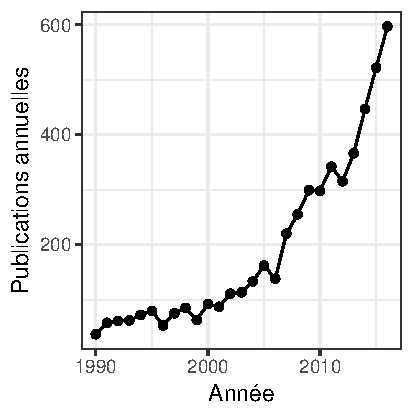
\includegraphics[height=5cm]{figures/WoS_IO.pdf}}
		\label{fig:WoS_IO}
	} \qquad
	\subfloat[Web of Science, résultats pour "Input-Output AND employment"] {
		\makebox[5cm][c]{
			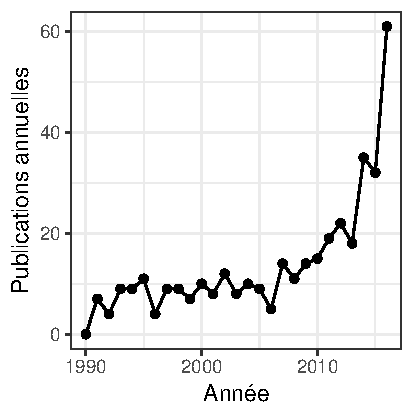
\includegraphics[height=5cm]{figures/WoS_IOEmployment.pdf}
		}
		\label{fig:WoS_IO_Environement}
	}
\end{figure}


\vspace{1em}
\textbf{La méthode de décomposition LMDI}

Les méthodes de décomposition d'indice permettent de déterminer l'importance de divers paramètres quant à l'évolution d'un agrégat. Par exemple, dans le domaine de l'énergie, l'évolution des émissions est souvent décomposé, selon l'équation de Kaya, entre quatre facteurs : l'augmentation de la population, l'augmentation du PIB par habitant, l'intensité énergétique et le contenu en carbone de l'énergie (cf. figure \ref{fig:kaya}). Quand les émissions augmentent d'une année à l'autre, les méthodes de décomposition d'indice permettent de comprendre les parts relatives joués par les différents facteurs. On peut alors comprendre si l'évolution des émissions est principalement tirée par la démographie, des effets de richesses, des progrès en efficacité énergétique ou des changements dans le bouquet énergétique.

\begin{figure}[!ht]
	\centering
	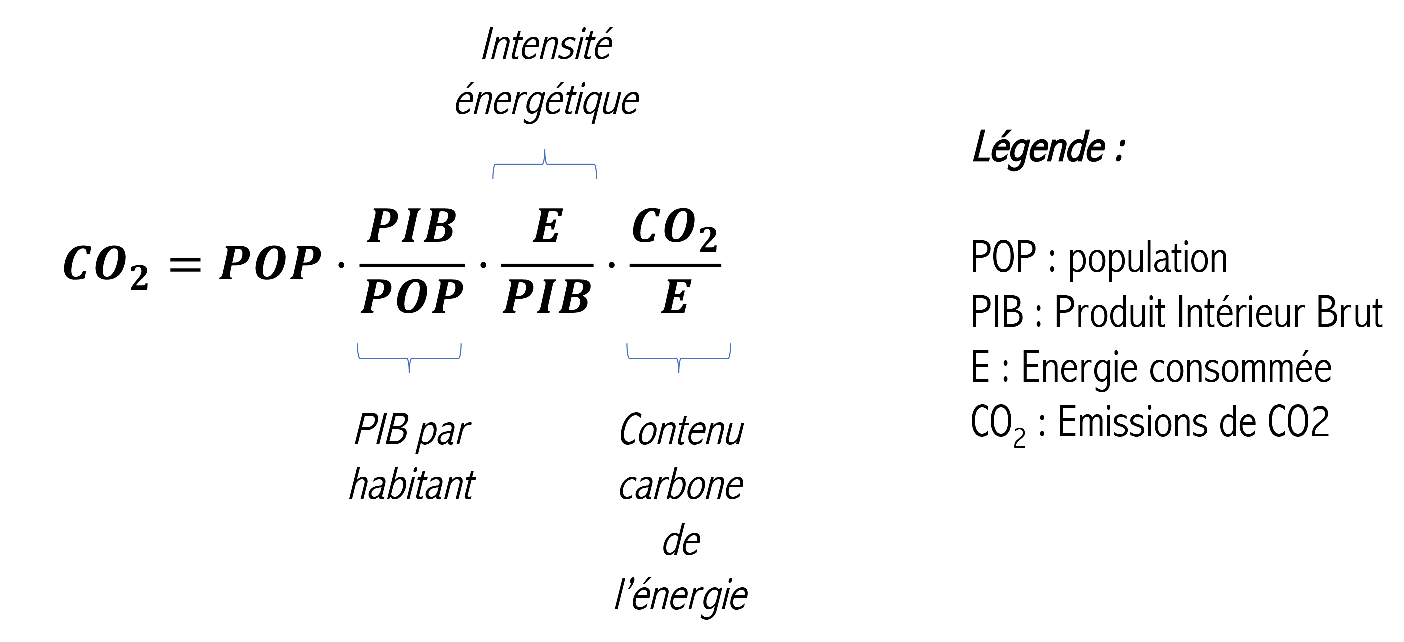
\includegraphics[width=10cm]{figures/Kaya.pdf}
	\caption[Décomposition de Kaya des émissions]{Décomposition de Kaya des émissions de \coo}
	\label{fig:kaya}
\end{figure}

En pratique, plusieurs méthodes de décomposition d'indice existent aujourd'hui. Parmi les plus connus, on peut citer les indices de Laspeyres, de Paasche et de Fischer, utilisés notamment pour calculer l'indice des prix à la consommation ; mais d'autres indicateurs existent. La raison pour cette pluralité de méthodes est qu'aucune décomposition n'est parfaite. Dans le domaine de l'énergie, la méthode LMDI popularisée par \citet{Ang2004} est de plus en plus utilisé. Le choix d'un indicateur est une discussion technique, mais le meilleur argumentaire me semble être celui de \citet{Muller}. Il réfute quelques arguments souvent utilisés, tout en proposant de nouvelles raisons pour préférer cet indicateur. En particulier, il montre que cet indicateur donne la meilleure décomposition pour toute une famille de fonctions usuelles.

En combinant la méthodologie Input-Output avec le LMDI, je cherche à décomposer le contenu en emploi des différents secteurs économiques. La première étape consistera à déterminer les facteurs qui composent le contenu en emploi, afin d'obtenir une décomposition formellement semblable à l'équation de Kaya.
La seconde étape sera de calculer l'apport de chaque des facteurs pour expliquer l'écart à la moyenne.

Par cette décomposition, je vise à comprendre les variations du contenu en emploi entre les différents secteurs économiques, notamment pour les secteurs concernés par la transition énergétique.
Par exemple, pourquoi le contenu en emploi de la rénovation est-il élevé ? Est-ce du fait d'importations faibles, d'une forte part du travail plutôt que du capital, de salaires faibles ? Quelle est la part relative de chacun de ces facteurs ? On peut se poser les mêmes questions pour les énergies renouvelables.
Selon la réponse à ces questions, les conséquences d'une politique favorisant ces secteurs seront très différentes : dans le premier cas, elles seront de réduire les importations ; dans le second, de favoriser les travailleurs au détriment des détenteurs de capital ; dans le troisième, de baisser les salaires pour créer de l'emploi. 
Ce travail d'analyse m'apparait donc essentiel pour mieux comprendre les implications économiques de la transition énergétique, secteur par secteur.



\subsection{Réallocation de la demande finale et création d'emplois: mécanismes économiques et résultats robustes}

\subsubsection{Une pluralité de résultats aux conclusions variées}

Les publications académiques sur le double dividende emploi sont nombreuses, mais les conclusions divergent et les mécanismes économiques sous-jacents sont peu clairs.
Après une première approche plus théorique, avec notamment l'article fondateur de \citet{Bovenberg1994a}, la littérature s'est essentiellement portée sur l'analyse empirique et numérique des effets d'une taxe environnementale. 
Cependant, les résultats de ces analyses diffèrent selon les types de taxe et les modèles utilisés. L'impact sur les émissions de CO\textsubscript{2}, le PIB et l'emploi varient fortement. Il est difficile de dégager des conclusions robustes de ces travaux. 

Une explication possible est la pluralité des objets étudiés, des politiques implémentées, et des types de modèles utilisés.
Pour l'objet d'étude, il y a une grande variabilité dans les pays, les années et les technologies considérées (système électrique, transports, bâtiment). 
La politique économique est généralement représentée par une taxe. Mais le point d'application de cette taxe peut varier (la taxe porter sur le carbone, sur le capital, etc), tout comme son mode de recyclage, c'est-à-dire la façon dont sont utilisés les revenus (baisse des cotisations sociales, redistribution directe aux ménages, etc.).
Enfin, les modèles utilisés appartiennent à différentes familles, avec des représentations différentes des équilibres macroéconomique. Dans ces familles, on peut citer notamment les modèles d'équilibre général (CGE), les modèles Input-Output et les modèles macroéconométriques.

Est-il possible de dégager au moins des résultats robustes par type de modèle ? 
Dans une méta-analyse d'études sur la taxe environnementale, \citet{Patuelli2005} montrent que l'emploi augmente souvent - y compris à long terme - mais que l'effet sur le PIB est plus ambigu. Mais ils estiment qu'il n'y a pas de conclusion robuste sur le type de modèle (macroéconométrique ou CGE) et de politique qui permette d'obtenir un double dividende. Les résultats ne tiennent donc pas uniquement au type de modèle, mais aussi à l'implémentation, aux hypothèses plus fines qui peuvent varier entre modèles de la même famille. Par exemple, les sensibilités des modèles aux variations de prix, donnés par les élasticités calibrées de façon exogène, peuvent aboutir à des résultats différents en termes d'exportations, ou de variations des salaires, ce qui peut \textit{in fine} avoir des répercussions importantes sur le résultat final en termes de PIB ou d'emploi.



\subsubsection{Comprendre les mécanismes économiques en jeu}


%Cette diversité de résultats, de scénarios et de modèles appelle plusieurs questions. Quels sont les résultats robustes d’un modèle à l’autre, et ceux qui divergent ? Et au-delà des résultats, quels sont les mécanismes qui aboutissent à la création d’emploi ? L’idée est, au-delà des modèles et des résultats quantitatifs, de pouvoir développer une compréhension des phénomènes économiques à l’œuvre. 

Mais au-delà des débats sur les résultats quantifiés, peu de discussion portent sur les mécanismes économiques à l'\oe{}uvre. Pourquoi telle politique économique génère de l'emploi, et pas telle autre ? 
Cette compréhension des mécanismes sous-jacents me parait cruciale. Le modèle doit être un outil d'aide à la compréhension. Il doit permettre de répondre à la question du \textit{combien}, mais aussi et surtout à celle du \textit{pourquoi}.
Cette discussion est essentielle pour distinguer les résultats robustes des artefacts qui proviennent purement d'un jeu d'hypothèses particulier et contestable.
Les hypothèses sur les opportunités à l'export, l'impact sur la compétitivité, la représentation du marché du travail ou encore la façon dont sont financés les investissements sont souvent peu discutées.

Par ailleurs, la question des investissements est peu relativement abordée dans la littérature. La majorité des travaux macroéconomiques s'intéressent aux impacts d'une taxe. Mais si la fiscalité carbone fait couler beaucoup d'encre (avec notamment l'EU ETS en Europe), on observe également un grand besoin d'investissement dans les infrastructures bas-carbone. 
Sortir du tout-pétrole dans les transports, isoler les bâtiments, installer des énergies renouvelables : renouveler les infrastructures nécessite un investissement initial important, et la taxe n'est pas l'unique, ni même nécessairement le meilleur moyen d'y parvenir. Les investissements sont un levier essentiel de la transformation de nos systèmes économiques. D'ailleurs, le programme du nouveau Président de la République, Emmanuel Macron, fait de son plan d'investissement public le «~bras armé~» de la transition énergétique et écologique \citet{Zaouati2017}. 

J'ai donc choisi d'étudier l'impact des investissements sur l'emploi. Plus précisément, j'ai décidé de me concentrer sur un type particulier de scénario : une réallocation des investissements. L'idée est de travailler à budget constant. Cette option peut être intéressante pour un décideur soumis à des contraintes de budget. Elle présente également l'avantage de ne pas entrer dans les discussions délicates sur le financement de ces investissements. Un résultat positif obtenu avec cette méthode sera donc d'autant plus fort : s'il est possible créer plus d'emploi à niveau de dépense égale, cette politique parait une bonne marche suivre.

\subsubsection{Méthodologie : les modèles d'équilibre général calculable}

Dans cette analyse, je me concentre sur deux types de modèles : les modèles d'équilibre général calculables (CGE) et les modèles Input-Output. Ces deux familles sont en effet parmi les plus utilisées pour les analyses en emploi de la transition énergétique.

Mon objectif est de faire une comparaison pas à pas, d'analyser l'impact de chaque équation ou bloc d'équations. Par exemple, le marché du travail et le commerce sont chacun modélisés par un bloc d'équations.
L'idée est de pouvoir ainsi déterminer quelles équations sont déterminantes, puis de discuter leur pertinence.

Je commence par mettre en évidence trois déterminants de la création d’emplois dans un modèle IO : le niveau des salaires, la part du travail dans la valeur ajoutée et le taux d’importations. Ces éléments ont un côté intuitif qui fait écho au débat public. Ils permettent en outre de faire le lien avec mon analyse sur le contenu en emploi. Mais sont-ils confirmés dans un cadre d’équilibre général ?

Pour tenter de répondre à cette question, je développe pour chaque mécanisme un modèle simple d’équilibre général à deux secteurs, une maquette permettant la comparaison avec le modèle IO. 
Ensuite, j’utilise un modèle CGE complet à 58 secteurs. 
Le modèle choisi est le plus standard possible : il s'inspire très largement d'un modèle présenté dans un manuel de macroéconomie : le \textit{Textbook of Computable General Equilibrium Modeling} \citep{Hosoe2010}. En outre, les équations du modèle sont publiées sur le site officiel de la communauté de modélisateurs GAMS. Ce choix d'un modèle standard est fait pour que les résultats et les mécanismes observés soient les plus généraux et les plus transparents possibles. Le but est d'éviter au maximum l'aspect «~boite noire~» souvent reproché aux modèles macroéconomiques.

Enfin, j'étudie deux politiques de façon quantitative avec le modèle CGE complet : l'installation de panneaux solaires et l'isolation thermique de bâtiments. La compréhension des résultats chiffrés devra pouvoir s'appuyer sur l'analyse des mécanismes réalisée avec les modèles stylisés.


%%%%%%%%%%%%%%%%%%%%%%%%%%%%

\section{Plan de la thèse}

Le plan de ma thèse s'articule autour de ces deux grands enjeux : le choix d'une stratégie de long terme et la question de l'emploi.
Il en résulte deux grandes parties pouvant être lues de manière relativement autonome.

La première partie correspondant au chapitre \ref{chap:nuclear_bet}. A travers le cas d'un secteur électrique français et la question de la prolongation des centrales nucléaires, j'étudie les questions d'incertitude et d'inertie en appliquant la méthodologie RDM à un modèle d'optimisation du parc électrique construit spécifiquement pour cette question : FLORE. 
Après une introduction du contexte, j'insiste d'abord sur l'amplitude des incertitudes existantes. Je présente ensuite le modèle FLORE et la méthodologie RDM. 
L'application conjointe des deux permet d'aboutir à des recommandations concrètes pour la politique publique, en lien les débats actuels sur le nombre de réacteurs à rénover. Je conclus en proposant de nouvelles stratégies pour le déploiement des renouvelables, qui me paraissent meilleures que les scénarios de référence proposés pendant le Débat National sur la Transition Energétique.

La seconde partie est composée des chapitres \ref{chap:TE_Emploi} et \ref{chap:mechanisms}. J'y explore les impacts sur l'emploi de la transition énergétique. La perspective est ici macroéconomique, et non plus sectorielle comme dans la partie précédente.
Dans le chapitre \ref{chap:TE_Emploi}, je m'intéresse plus particulièrement à la notion de contenu en emploi des différents secteurs économiques. En croisant l'intensité en emploi et l'intensité en émissions de GES, à l'aide d'une méthode de type Input-Output, je donne une vision des secteurs qui semblent les plus favorables à une transition écologique et sociale. Je propose ensuite une méthode nouvelle pour décomposer le contenu en emploi, afin de mieux en saisir ses composantes et leur importance relative : taux d'importations, part du travail dans la valeur ajoutée, niveau des salaires ou montant des taxes et subventions. Ma décomposition montre que les taxes induisent un effet distorsif dans cette métrique, et permet de corriger cet effet. Elle aide en outre à mieux cerner les effets à l'\oe{}uvre dans les modèles macro-économiques.

Je poursuis cette réflexion sur les causes et les mécanismes économiques présidant à la création d'emploi dans le chapitre \ref{chap:mechanisms}. J'étudie spécifiquement le cas d'une réallocation de l'investissement, en mobilisant des modèles de type CGE et Input-Output. Je montre que trois facteurs sont à la source d'une évolution de l'emploi : le taux d'importations, la part du travail dans la valeur ajoutée et le niveau des salaires. Cette mise en évidence dans les équations des modèles fait donc le lien avec la décomposition descriptive du chapitre précédent. Mais cette partie met aussi en évidence un effet plus ambigu des importations : encourager les secteurs faiblement importateurs a des effets très positifs en Input-Output, et beaucoup moins dans les modèles CGE. Enfin, je réalise l'évaluation quantitative de deux politiques publiques : investir dans l'isolation des bâtiments et les panneaux solaires PV privés. Je montre que dans ces deux cas, l'impact sur l'emploi est positif grâce à la forte part de travail dans la valeur ajoutée et le faible niveau des salaires, et que ce résultat est robuste à travers les deux familles de modèles. 

Pour finir, je présente les conclusions de ma thèse dans le chapitre \ref{chap:conclusion}. Je replace mes résultats dans une perspective plus large, avant d'ouvrir des pistes sur les possibles améliorations et recherches futures.






\phantomsection
\printbibliography[heading=subbibintoc]

\newrefsection
\selectlanguage{english}
\chapter{The French nuclear bet} \label{chap:nuclear_bet}

%%%%%%%%%%%%%%%%%%%%%%%

\section{Introduction} \label{sec:introduction_chap2}
The first oil shock provoked the engagement of France in an unprecedented nuclear program, which would make it up to now the country with the highest share of nuclear in its power mix.
The first Contract Program was launched in 1969. A batch of six reactors of 900 MWe was ordered (the CP0 batch) and their construction started in 1971. But the 1973 oil embargo triggered a more ambitious nuclear program. In early 1974, 18 identical reactors of 900 MWe were ordered (CP1 batch). They were followed in late 1975 by 18 new reactors: 10 reactors of 900 MWe (CP2 batch) and 8 of 1300 MWe (CP4 batch). 12 additional reactors of 1300 MWe were ordered in 1980 (P'4 batch). Finally, in 1984, 4 reactors of 1450 to 1500 MWe (N4 batch) concluded this nuclear policy \citep{Boccard2014}.
These massive orders have shaped power production in France ever since. In 2015, these nuclear plants produced 78\% of the country's electricity. Along with a 12\% of hydropower production, it leaves only around 10\% for all other sources of power \citep{RTE2014}.

But these power plants are now reaching the end of their lifetime. The reactors were initially designed to last for 32 years at nominal power and 40 years at 80\% of their nominal power \citep[p. 31]{Charpin2000}. In practice, the 40-year threshold is used by the national authority on nuclear safety, the ASN. These reactors are now reaching this 40-year limit. The first ones will be the two reactors in Fessenheim, which will turn 40 years old in 2017.

The lifetime of these nuclear plants can be extended if retrofit works are undertaken. 
A new report by the French 'Cour des Comptes'\footnote{
	The Court of Auditors (in French Cour des Comptes) is a quasi-judicial body of the French government charged with conducting financial and legislative audits of most public institutions} 
estimated at \euro 100 billion the cost of retrofitting the plants up to 2030 \citep{CourdesComptes2016}. Should all plants be retrofitted? And more generally, what is the future of nuclear energy in France?
These questions are now at the heart of public debate. The diversity of opinions on this matter was highlighted by the French National Debate on Energy Transition in 2012. The views on the future of nuclear generation in France ranged from a fully maintained nuclear share, to partial retrofit strategies, to a full and early phase-out \citep{DNTE_gt2}. 

France is now at a crossroad. The economics of this decision crucially depend on the cost of nuclear, both new and retrofitted; but these are subject to significant uncertainty. A combination of recent setbacks in the nuclear industry has raised some doubt about the future cost and safety of this technology.
For new nuclear reactors, the most famous example is the significant cost overrun of the EPR at Flamanville (France). The project was initially estimated at \euro 3 billion, but this estimate has increased progressively up to \euro 10.5 billion in 2015 \citep{Garric2015}, and there are still concerns about the safety of its vessel \citep{Hir2015}. For retrofitted nuclear, the estimation may also be optimistic, as unexpected delays often occur in such megaprojects. For example, in the plant of Paluel, the replacement of steam generators has led to the fall of one steam generator of 465 tonnes, which requires safety inspection and will cause delays \citep{ASN2016}. Safety concerns about current vessels have also led to stopping nuclear reactors in winter, threatening security of supply \citep{Monicault2016}.

Other uncertainties must also be accounted for, in particular those concerning the level of demand and \coo\ price. The level of demand can be affected by economic growth or downturn, by energy efficiency and the development of new uses like electric cars. \coo\ price can impact the relative competitiveness of gas and coal, but also renewables backed up by gas. This \coo\ price depends on political will, which is difficult to anticipate.

Given these uncertainties, what are the policy options available, and what are their risks and benefits? 
The current debates suggest that there is no silver bullet, no single optimum strategy for all plausible values. Thus, we aim to find a robust strategy, i.e. a strategy that "performs relatively well --compared to alternatives-- across a wide range of plausible futures" \citep{Lempert2006}. 
%Our aim is also to identify trade-offs between possible strategies and the vulnerabilities of each strategy -- that is, combinations of model parameters in which the strategy performs relatively poorly. 
To do so, we combine the cost-minimizing optimization model of the French power sector FLORE with the framework of Robust Decision Making \citep{Lempert2006}, in a way similar to \citet{Nahmmacher2016}. This RDM framework combines scenario-based planning with statistical analysis, in order to identify robust strategies, vulnerabilities and trade-offs. We apply it to the results of nearly 3,000 runs made with the FLORE model. 
Our paper aims to provide insight for the current debate in France concerning the retrofit of existing nuclear plants. More generally, it also explores the importance of uncertainties related to nuclear energy in power system planning, and could thus contribute to the debates in other European countries, in particular Germany and Switzerland.

In section \ref{sec:plausibleValues}, we examine in detail the ranges of uncertainty. These ranges will be used for the parameters of our model FLORE, which is introduced in \ref{sec:modelDescription}. We present the RDM framework in sections \ref{sec:method} and apply it in section \ref{sec:results} to identify robust strategies. Finally, we compare our results to the French official scenarios in section \ref{sec:comparison}. Section \ref{sec:conclusion2} outlines the conclusions.


%%%%%%%%%%%%%%%%%%%%%%%%%%%
%%%%%%%%%%%%%%%%%%%%%%%%%%%%%%%%


\section{The uncertainty ranges in the literature}
\label{sec:plausibleValues}

\subsection{Overview}
Various elements stretch the range of plausible future costs for both retrofitted and new nuclear.

On one hand, the recent literature and events about nuclear costs presents arguments supporting the idea of increasing costs in the future:
\begin{description}
	
	\item [Negative learning-by-doing] The French nuclear industry has been facing "negative learning-by-doing" in the past, although it benefited from a very favourable institutional environment \citep{Grubler2010}.
	
	\item [Increased regulatory pressure on safety] Increased regulatory pressure can increase costs \citep{Cooper2011}. In particular, the Fukushima accident has led the French nuclear regulator, the ASN, to impose new safety measures.
	
	\item [Recent and unexpected cost surge]: the EPR technology in Flamanville (France) has been delayed several times, and its cost tripled.
	The EPR in Olkiluoto (Finland) is also facing several difficulties.
	This is raising doubts about the ability of EDF to build power plants of the EPR technology.
	As to retrofitting the historic power plants, the first retrofit has led to an incident which may cause delays and significant cost increases\footnote{
		on March 31, 2016, a steam generator of 465 tonnes and 22m high fell during its replacement operation};
	
	\item [High contract price for nuclear] In the UK, EDF signed a contract at 92.5~\pounds/MWh (127~\euro/MWh at 2015 exchange rate of Eurostat\footnote{\url{http://ec.europa.eu/eurostat/web/exchange-rates/data/main-tables}}) and indexed on inflation, which means the nominal price will be higher when the plant starts to produce. The exact costs of the French EPR are difficult to assess as they are not publicly displayed. This market price is thus an important clue as to the cost of this technology.
	
	\item [Unexpected stops] The discovery of anomalies has led to reinforced controls. As a consequence, in October 2016, 12 reactors out of 58 were stopped to check the resistance of their steam generators \citep{Monicault2016}. This lead to concerns about the security of supply and the future load factor of these plants, which is a key parameter of their value \citep{IEA2015}.
	
	\item [Risks and insurance costs] The Fukushima accident prompted a renewed interest on the question of insurance costs from the French court of audit \citep{CourdesComptes2012}. This insurance should match the criticality of nuclear, i.e. the probability of an accident multiplied by severity of the consequences. Up to now, the French nuclear operator EDF has benefited from a limited liability. But both probability and damage costs are difficult to estimate. To give an idea of these uncertainties, \citet{Boccard2014} estimates this insurance cost at 9.6 \emwh, while \citet{Leveque2015} provides an expected cost below 1 \emwh. 
	
	\item [Decommissioning and waste management] No decommissioning has been finished yet, so the total cost is difficult to estimate. The first nuclear installation to be decommissioned in France, Brennilis, saw its cost multiplied by twenty compared to initial estimates. And in a novel report, a commission of the French Parliament reckons that the cost of dismantling might be underestimated in France \citep{AN2017}.
	As to waste management, a project called Cigeo is planned to store highly radioactive long-lived wastes. Its cost was estimated at between 15,9 and 55 billion euros in 2002 by the national radioactive waste management agency, ANDRA \citep[p. 142]{CourdesComptes2012}.
	
\end{description}

On the other hand, constructing several reactors of the same type can lead to learning-by-doing in the construction process. Standardization reduces lead times and thus reduces the cost of this technology. The size of reactors is also positively correlated with cost \citep{Rangel2015}, so a standardized approach with smaller reactors could thus stop the negative learning-by-doings and even decrease the future costs of nuclear.

These elements should encourage carefulness when assessing the future costs of nuclear. They entail that a wide range of costs can be considered as \textit{plausible}, in the sense that they cannot be immediately dismissed since some elements support them. In the next sections, we examine what could be the future cost of retrofitted and new nuclear, based on the current literature.


\subsection{Cost of retrofitted nuclear plants}

\subsubsection{Historical costs}

The cost of the French nuclear reactors has been the focus of a few papers.
The first official report on the historic French nuclear program was made by \citet{Charpin2000}.
It was later analyzed by \citet{Grubler2010}, who evidenced cost escalation in time, which he coined as "negative learning-by-doing".
After the Fukushima accident, the French court of audits undertook a comprehensive analysis of the costs and safety of French nuclear reactors. Based on this report, \citet{Boccard2014} revealed larger than expected operation costs for French reactors: 188 \euro/kW/year, or 28.5 \emwh\ with the historical load factor. This value is a key determinant of the cost of retrofitted nuclear, since fixed capital costs are already amortized to a large extent. And this estimate is much higher than the value suggested by \citet{IEA2015} at 13,3 \emwh.
Using the same report, \citet{Rangel2015} also noticed a cost escalation, but revealed a learning curve within technologies of the same type and size.


\subsubsection{Costs of retrofitting}
These old reactors now reach the end of their planned lifetime, initially intended to be 40 years\footnote{
	French reactors were initially designed for a lifetime of forty years, with a count start at their first nuclear reaction. In the US, lifetime is counted from the first layer of concrete.
}.
These lifetimes can be extended, but only if some upgrade work is performed. A new report published by the French court of audit \citep{CourdesComptes2016} provides the costs estimated by EDF\footnote{Electricité de France, the main operator of the nuclear fleet in France.} to retrofit its nuclear fleet and bring safety up to post-Fukushima standards. According to EDF, an investment of \euro 100B is required by 2030: 74.73 in CAPEX and 25.16 in OPEX \citep{CourdesComptes2016}.
Between 2014 and 2030, 53.2 GW will reach 40 years, yielding an average additional cost of 1,404 \euro/kW.

In addition to these overnight capacity costs, the cost per unit of energy produced is influenced by capital cost, load factor and lifetime.

Financial costs are highly dependent on the rate at which capital is borrowed. 
In France, \citet{Quinet2013} recommends to use a rate of 4.5\% for public investments.
The IEA uses a rate of 5\%, which we use for our best-case scenario, to account for financial costs.
We use a rate of 10\% for our worst-case scenario, following \citet{Boccard2014}.

For the load factor, we use a best case based on the estimates by \citet[p. 116]{CourdesComptes2016}, which shows that the availability of French nuclear plants has been up to 83.5\% since 2005. In 2012, the load factor was down to 73\% in 2012, but considering the recent difficulties faced by French reactors, we use a load factor of 70\% as a worst case.

As to lifetime, we suppose that the investment of \euro 100B will enable the plant to run for 20 more years. This is currently the implicit assumption of EDF \citep[p. 13]{AN2017}, but there is significant uncertainty around this hypothesis. In France, nuclear plants are given license by periods of ten years. 
The French Authority of Nuclear Safety (ASN) seems willing to provide licenses for a ten year extension; but there is no certainty that it will give a second approval, ten years later, to go beyond fifty years of operation. 
It may decide to close some plants, or ask for additional investment at that time. However, the magnitude of the investment indicates that EDF is confident it will be able to run for twenty more years without incurring in large additional costs. Thus, this is our best-case hypothesis. We consider a worst case in which lifetime extension will be granted for ten years only. 


\subsubsection{Cost of a nuclear accident}
\label{ssec:accident}

The Fukushima accident has prompted a renewed interest on the question of insurance costs. The insurance cost should match the criticality of nuclear, i.e. the probability of an accident multiplied by severity of the consequences. However, both the probability of an accident and damage costs are difficult to estimate.

Damage costs depend on several assumptions about indirect effects, as well as on monetizing nature and human lives \citep{Gadrey2016}. Thus, an irreducible uncertainty remains here. To give an idea of these uncertainties, the Institute for Radiological Protection and Nuclear Safety (IRSN) estimated the cost of a "controlled" release of radioactive material between 70 and 600 billion euros \citep{CourdesComptes2012}. To give another reference, the Fukushima accident has been estimated at 160 billion euros by \citet{MunichRe2013}.

To assess the probability of a nuclear accident, two approaches coexist. The first one is the Probabilistic Risk Assessment (PRA). It consists in a technical bottom-up approach, which compounds the probabilities of failures which could lead to a core meltdown. This measure is used by regulators in the US \citep{Kadak2007}. Depending on regulators, this PRA varies from 10\textsuperscript{-4} to 10\textsuperscript{-6} per year and per reactor \citep{Ha-Duong2014}. In France, the probability of an accident which would release a significant amount of radioactivity in the atmosphere is estimated at 10\textsuperscript{-6} for current plants, and 10\textsuperscript{-8} for the EPR reactor \citep{CourdesComptes2012}. However, some uncertainty remains within the information that is not fully captured by this type of analysis, as suggested by the examples of Three Mile Island, Chernobyl and Fukushima. A wide discrepancy is observed at first glance between the expected number given by the PRA estimate and the number of observed nuclear accidents worldwide \citep{Ha-Duong2014}. 

This discrepancy has motivated another approach, based on the statistical analysis of past historical accidents. In particular, the Fukushima accident has prompted a renewal of research based on empirical estimates. \citet{Rangel2014} recall that most of the accidents occurred at the early stage of nuclear power plants. Continuous safety improvements might have improved security and brought it closer to PRA estimates. They also argue that the Fukushima accident has revealed the risks associated with extreme natural events and regulatory capture, thus opening the door for further improvements.

However, this second approach suffers from two short-comings. The first one is the low number of occurrences. Only two events are classified in the category of major accident, i.e. a level 7 on the INES scale - the INES scale, introduced by the International Nuclear Energy Agency, ranges nuclear events from 1 (anomaly) to 7 (major accident). Such a small sample hinders robust statistical analysis. Most studies thus estimate the probability of a larger pool of events by including events lower on the INES scale, but the gain in estimation accuracy comes at the cost of a change in the meaning of the results \citep{Rangel2014}. What is measured is not only the probability of major accidents occurring, but it also includes the probability of less dramatic events. 
The second shortcoming comes from the use of past, historical data. This does not enable to account for the potentially increased risks due to aging power plants, nor for the tense political situation with fears of terrorist attacks. 
This uncertainty can drastically change the cost of insurance. If we estimate the cost of insurance should match the criticality of nuclear, and if we assume the cost of a major nuclear accident to be 100 billion euros, as recommended by \citet{CourdesComptes2012}, then a probability of accident between 10\textsuperscript{-7} and 10\textsuperscript{-6} makes the insurance cost vary from 1.4~\emwh\ to 14.2~\emwh, as shown in table \ref{tab:insurance}. 
And that range is in line with the requirement from the regulator for a core meltdown.

The point behind these figures is that the cost of insurance cannot be dismissed once and for all. Expectations of security improvements can explain an almost negligible value for nuclear insurance, while a more conservative view can lead to significantly higher estimates, up to 14 \emwh. 

\begin{table}
	\centering
	\caption{Estimated nuclear insurance costs for a damage cost of 100 billion euros.}
	\label{tab:insurance}
	\begin{tabular}{p{2cm}p{6cm}}
		\toprule
		Estimated probability of an accident \newline (per MW per annum) & Insurance cost (euro/MWh) \\
		\midrule
		$10^{-8}$  & 0,14 \\
		$10^{-7}$  & 1,43 \\
		$10^{-6}$  & 14,27 \\
		$10^{-5}$  & 142,69 \\
		\bottomrule
	\end{tabular}  
\end{table}


\subsubsection{Decommissioning and waste management costs}

A novel report by the French Parliament provides several clues as to the uncertainty surrounding decommissioning costs. 
Brennilis, an experimental reactor built in 1962, marks the first decommissioning of a nuclear power station in France. Although not achieved yet, the cost of decommissioning is currently estimated to be 482 million euros, around twenty times its initial estimate \citep{AN2017}.
This evolution leads to be cautious with the current cost assessments of other nuclear installations.
Even the technical feasibility of decommissioning is not granted yet. This is illustrated by the decision of EDF to postpone to 2100 the decommissioning of several experimental nuclear installations in order to have the time to develop new technologies for a safe decommissioning \citep{AN2017}.
Finally, there is a large divergence between the estimates of European operators. The accounting provision is generally between 900 and 1.3 billion euros per reactor, EDF's provision is only 350 million euros per reactor \citep{AN2017}. The argument of standardization is used to justify this lower cost estimate.
But due to the significant difference with other European operators, we also consider a worst-case scenario in which a doubling of current costs and provisions cannot be excluded.

As to waste management, a facility called Cigeo is planned to be built to serve as a repository for highly radioactive long-lived wastes. The cost of this project was estimated at between 15,9 and 55 billion euros in 2002 by the national radioactive waste management agency, ANDRA \citep[p. 142]{CourdesComptes2012}.
Since these costs will be incurred in a distant future, valuing this nuclear liability depends on the choice of a discount rate. \citet{Taylor2008} estimates a risk-free rate should be used. 
In France, the discount rate is fixed by the application decree 2007-243 of 23 February 2007 relative to ensuring the financing of nuclear accounting charges\footnote{décret 2007-243 du 23 février 2007 relatif à la sécurisation du financement des charges nucléaires}. 
The nominal rate must be lower than a four-year moving average of government bonds of constant maturity at 30 years, plus a hundred base points \citep[p. 110]{CourdesComptes2014}. This rate is subject to market fluctuations, which impacts the amount of accounting provisions and thus the cost of nuclear.
However, an increase in the cost of Cigeo from 16.5 to 36 billion euros would only increment generation costs by 1\% \citep[p. 282]{CourdesComptes2012}. This small sensitivity is due to the effect of discounting long-term costs. Given the uncertainty on costs and discounted rate, we consider another doubling of cost as our worst-case scenario.

In conclusion, decommissioning and waste management costs add another layer of uncertainty to generation costs. However, their overall impact, without being negligible, is mitigated by the discounting effects.


\subsubsection{Summing up}
Overall, there are at least eight sources of uncertainty for retrofitted reactors: the overnight capital cost of retrofitting, the cost of borrowing, the future OPEX, the length of lifetime extension (10 or 20 years), the future availability of nuclear plants and the costs of waste, decommissioning and insurance.
Using the most recent data available, detailed in tables \ref{tab:historical_costs} and \ref{tab:costs_grand_carenage}, we compute that, in the best case, the cost of retrofitted nuclear would be 44 \emwh. But based on conservative assumptions detailed in table \ref{tab:sensitivity_tests} in appendix, various sources of uncertainty could amount to an additional 51.5 \emwh. Plausible values for this technology thus range from 44 \emwh\ to 95.5 \emwh.


\begin{figure}[!ht]
	\centering
	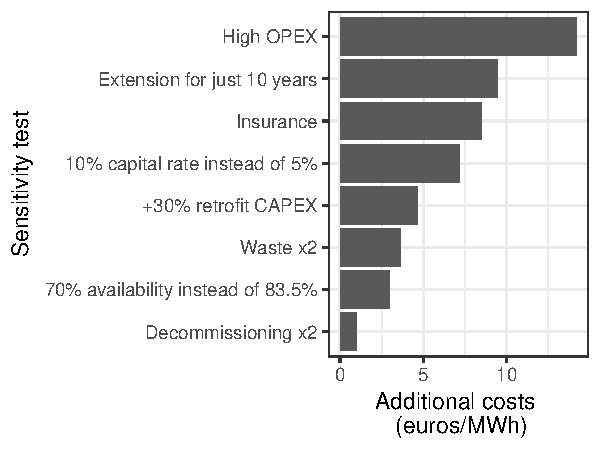
\includegraphics[height=5cm]{figures/sensitivity_tests.pdf}
	\caption{Plausible additional costs for retrofitted nuclear compared to a best case of 44 \emwh}
	\label{fig:sensitivity_tests}
\end{figure}

\subsection{Cost of new nuclear plants}

In parallel to retrofitting its existing reactors, EDF has developed a new technology: the European Pressurized Reactor (EPR).
However, this model has also faced serious setbacks.
The yet unfinished reactor developed in France saw its cost rising from \euro 3 billion to \euro 10.5 billion.
In Finland, the construction work for an EPR reactor started in 2005 with a connection initially scheduled in 2009, but has so far been delayed until 2018.
In the UK, the EPR has been negotiated at 92.5 \pounds/MWh -- approximately 127 \euro/MWh at the exchange rate of 2015 given by Eurostat.

As to the future of the EPR cost, a tentative cost is estimated by \citet{Boccard2014} between 76 and 117 \emwh, for a total cost of \euro 8.5 billion (before its upwards adjustment to \euro 10.5 billion) when including back-end and insurance costs (he estimates insurance costs at around 9.6 \emwh). 
The high end is in line with the contract price of the Hinkley point reactor. A wide spread is found in the literature, from 76 \euro/MWh to 120 \euro/MWh.
In addition, the cost of nuclear has been shown to depend on safety pressure. For example, \citet{Cooper2011} showed that the Three Mile Island accident had a significant impact on cost escalation.
Consequently, any new incident could increase these current estimates. This creates additional uncertainty on future nuclear costs.
These significant uncertainties about future costs led some to qualify the nuclear option as a "bet" \citep{Leveque2013}.

This wide range of nuclear cost is critical, as it encompasses the current levels of feed-in tariffs for wind in France and its LCOE\footnote{
	The Levelized Cost of Electricity, or LCOE, is an economic assessment of the average cost of one unit of energy produced by a power-generated asset. It is equal to total discounted costs divided by total discounted generation over the lifetime of the asset.}
expected in 2050. 
In France, in 2014, onshore tariff was set between 55 and 82 \euro/MWh for a lifetime of 20 years (82 \euro/MWh for the first ten years, and between 28 and 82 \euro/MWh afterwards, depending on wind conditions)\footnote{
	Note that the wind developer must pay for connection to and upgrade of the distribution network to access this FIT.
}.
Wind tariffs in neighboring Germany were set at 59 \euro/MWh in 2015: 89 \emwh\ during 5 years and 49.5 \emwh\ afterwards \citep{EEG2014}.

Finally, it is important to note that new nuclear is expected to be costlier than retrofitted plants. The general idea is that a brown field project (a retrofitted plant) requires less investment than a greenfield project. Thus, we will focus on the cases in which new nuclear is costlier than retrofitted nuclear.


\subsection{Demand, CO2 price and renewable cost}
\label{subsec:demand}

There is some uncertainty on the demand level. This was highlighted during the National Debate on Energy Transition in France, which led to four contrasted demand scenario: SOB, EFF, DIV and DEC, in order of increasing demand (see figure \ref{fig:DNTE_scenarios} in appendix). 
Our reference scenario is in line with the DIV scenario, as it is closest to current projections by the French transmission line operator, RTE. It is roughly a scenario of flat demand. The most extreme scenarios were SOB, for low demand, and DEC, for high demand. We use these as our low and high case respectively, to account for all plausible values of demand.

For \coo, we use the official price used in French public investments as defined in \cite{Quinet2009}. In the central scenario, this price goes up to \euro 100 in 2030 to \euro 200 in 2050. In the short term, these prices are significantly higher than the price of emission allowances on the EU ETS market (which has stayed below 10 \euro/\coo\ on the EEX market in the past year) and there is no reason to think that the EU ETS price might be higher, even with the proposition of back-loading some allowances in the future \citep{Lecuyer2016}. 
We also consider a variant with low \coo\ price, in which we divide the official price by a factor of 2. 
It thus attains 50 euros in 2030 and 100 euros in 2050. Such a high price reflects the implicit view in all scenarios to phase-out coal and gas in the long-term, in order to avoid an increase of \coo\ emissions. They could also represent the price floor for \coo\ currently discussed in France. 

All these uncertainties thus raise the question of the optimal mix. However, the LCOE metric does not account for "integration costs" \citep{Ueckerdt2013}. 
Nuclear has the advantage of being a dispatchable power source, while wind and solar PV are variable. As a consequence, their value decreases as their penetration rate increases, although the magnitude of this decrease is specific to the power system \citep{Hirth2016a} and to the renewable technology characteristics \citep{Hirth2016}. This phenomenon of value drop is sometimes called "self-cannibalization effect". Using an optimization model of the entire power system enables us to capture these integration costs. Indeed, since the model finds the power system that satisfies demand at the least cost to society, wind or solar would only be installed if they are competitive.


\subsection{Related literature on power transition and nuclear}

Many studies have analyzed a low-carbon transition in the power sector, at a national level \citep{Fraunhofer2015} or a European level \citep{Jagemann2013, EuropeanCommission2012}. 
Focusing more specifically on nuclear, \citet{Bauer2012} study the cost of early nuclear retirement at world level, and show that the additional cost of enforcing a nuclear phase-out is an order of magnitude lower that the total cost of a climate policy. But this result might not hold true for France as the share of nuclear is much higher than the world average.

\citet{Linares2013} analyze the break-even overnight cost of nuclear, using an optimization model of the Spanish power sector. They come up with a medium estimate of 2,609 \euro/kW, and conclude that the cost-competitiveness of this technology is questionable given the cost estimates of new projects.

In France, the French Energy Agency, ADEME, produced a study of renewable penetration in 2050 \citep{ADEME2015}. However, they do not study the path between today and 2050: the power mix was built ex nihilo (greenfield optimization) in 2050 as an optimization with 2050 projected costs.
\citet{Petitet2016} study wind penetration in France, but without modeling the potential of hydro optimization to smooth wind penetration, and consider only cases in which nuclear is cheaper than wind - a debatable assumption, as we will show.

The uncertainties of power system planning have recently been emphasized by \citet{Nahmmacher2016}, who studies unplanned shocks in power systems using the same methodology as in this paper. But their study does not deal with unexpected costs of nuclear plants.

Our paper contributes to the literature in several points. The first and main one is to use a methodology of robust decision making to deal explicitly with the high uncertainty on nuclear costs. The literature as a whole shows a wide uncertainty on nuclear costs. Rather than using specific -- and controversial -- values, we propose a methodology to include this uncertainty in the decision-making process. This is an improvement compared to the pure cost-minimization, thresholds-based or sensitivity analyses. In addition, we provide new estimates on the cost of nuclear retrofit based on a novel report by the French government and, include a retrofit option in our analysis, rather than focusing on new plants. We also provide a model to study nuclear and renewables with around 12\% hydro and optimized pumped storage, while the literature has focused mainly on thermal power systems, and seldom on power system with a high share of hydro \citep{Hirth2016a, Linares2013}. Finally, we provide trajectories of nuclear for France, which is often difficult to represent properly in models covering a larger region because of its large nuclear fleet.



The next section introduces the model we use for our analysis.


%%%%%%%%%%%%%%%%%%%%%%
%%%%%%%%%%%%%%%%%%%%%%%%%%%

\section{Model description} \label{sec:modelDescription}

The French power model FLORE (\textit{French Linear Optimization for Renewable Expansion}) is an optimization model of investment and dispatch. It is based on representative technologies, with a particular focus on nuclear and hydropower modelling to reflect the specificities of the French power mix. All technologies are endogenous for both investment and dispatch, except for hydro capacities. Existing nuclear plants may be retrofitted for 20 years when they reach 40 years old, or they are decommissioned. Hydro resources from dams and pumping stations are dispatched optimally. In addition, all capacities are jointly optimized over the horizon, in order to provide a consistent trajectory of investments. France is represented as a single node. Hourly demand, net exports and \coo\ prices are exogenous. 

All the equations of the model are available for download at my professional webpage: \url{http://www2.centre-cired.fr/PERRIER-Quentin}. 
In addition, an interactive online version of the model can be found at \url{https://flore.shinyapps.io/model/}. 
This open access to all equations and data should ensure transparency and reproducibility, as advocated by \citet{Pfenninger2017}.

\subsection{Generation technologies}

Twelve generation technologies are modeled: two renewable energies (onshore wind and solar PV), three fossil-based thermal technologies (coal plants, combined cycle gas turbine, open cycle gas turbine), three nuclear technologies (historical nuclear, retrofitted nuclear and new nuclear) and three hydro systems (run-of-river, conventional dams for lakes and pumped storage).
Investment in each technology is a choice variable of the model, except for hydropower and historical nuclear, which are exogenous.
Generation of each technology is a choice variable, except for run-of-river production, which is exogenously based on historical data.

The capacity of run-of-river and conventional dams is supposed to be constant, while the pumped hydro capacity is supposed to grow by 3.2~GW by 2050, with a discharge time of 20 hours, as in \citet{ADEME2013}.
Hydro storage and dispatch is optimized by the model, under water reservoir constraints and pumping losses.
Dams receive an amount of water to use optimally at each period.
Pumped hydro can pump water (although there are losses in the process), store it into a reservoir and release the water through turbines later on.

A particularity of the model is to represent explicitly the cost of extending the lifetime of nuclear power plants.
Nuclear plants normally close after 40 years, but their lifetime can be extended to 60 years, if upgrade costs are paid for.
For historical nuclear, we model a phase-out of the capacity of each power plant reaching 40 years.
The same year it reaches 40 years, this capacity of a historical nuclear plant is endogenously either extended for 20 years, or phased-out. 
Thus, each year, total investment in retrofitted plants is limited to the capacity of historical nuclear reaching forty years.

Hourly Variable Renewable Energy (VRE) generation is limited by specific generation profiles based on historical data for the year 2014.
Dispatchable power plants produce whenever the price is above their variable costs, unless they are limited by their ramping constraints.
At the end its lifetime, each capacity is decommissioned.
Power generation required for heat generation was on average 2\% of consumption, and never above 5\% of consumption in France in 2014 \citep{RTE2014}, so we do not model it.
The remaining capacity can be optimized for power generation.

\subsection{Model resolution}

The model optimizes new capacities at a yearly step from 2014 to 2050. The dispatch of generation capacities is computed to meet demand for six representative weeks at an hourly step. Each typical week represents the average demand of two months of real data, through 168 hours. For example, demand of Monday for week 1 represents the average demand, on an hourly basis, of all the Mondays in January and February. This is similar to having 24*7=168 time slices in the TIMES model\footnote{http://iea-etsap.org/docs/TIMESDoc-Intro.pdf} or in the LIMES-EU model\footnote{https://www.pik-potsdam.de/members/paulnah/limes-eu-documentation-2014.pdf}.
Demand is exogenous and assumed to be perfectly price inelastic at all times. Net export flows are given exogenously, based on historical data. 
The various demand scenarios we study represent the initial demand profile (domestic consumption plus exports) and change it homothetically, thus without altering the shape of peak or base demands.

The model covers France as a single region.
Each typical week is associated with i) a water inflow for run-of-river and dams, ii) an availability factor for conventional generation technologies for each representative week, to account for maintenance and iii) a production profile for renewable technologies (onshore wind and PV) based on historical production.

\subsection{Objective function}

The objective of the model is to minimize total system costs over the period 2014-2050.
The cost of each technology is annualized, both for O\&M and capital costs. 
Capital annuities represent the payment of the loan. 
In addition, using annuities allows us to avoid a border effect in 2050: the annual costs are still well represented at the end of the time horizon.

We use a 0\% rate of pure time preference, in order to give the same weight to the different years and generation up to 2050. This assumption is also made in the EMMA model \citep{EMMA} used for example by \citet{Hirth2016}.
Costs include investment costs, fixed O\&M costs, variable costs and costs due to ramping constraints.
To account for financing cost (e.g. the cost of borrowing), investment costs are annualized with a 5\% interest rate, as in \citet{Jagemann2013}.
Variable costs are determined by fuel costs, CO\textsubscript{2} price, plant efficiency and total generation.

In section \ref{sec:plausibleValues}, we studied the range of plausible values for nuclear, highlighting eight sources of uncertainty. Looking at these specific cost items was necessary to understand the range of plausible costs for retrofitted nuclear, but we will not detail each of these items in our model, as it would lead to too many possibilities (and possibly overlapping ones). Instead, we will keep the OPEX fixed and make the CAPEX vary to cover the uncertainty range. This simplified approach allows a decision maker to use its own assumptions about each cost item, and use the resulting cost in euro per MWh to interpret our results.

All assumptions regarding investment costs (table \ref{tab:Investment _costs}), fixed O\&M costs (table \ref{tab:OM_costs}), CO\textsubscript{2} price (table \ref{tab:CO2_price}), fuel prices (table \ref{tab:Fuel_prices}) and net efficiencies (table \ref{tab:Efficiencies}) can be found in appendix \ref{app:calibration}.

\subsection{Scope and limitations}

The objective function does not include grid costs explicitly.
However, for wind, the feed-in tariff we use includes grid connection costs, through the 'quote-part' paid by the wind developer to the network operator ERDF.
For nuclear plants, they will be most likely built on sites with grids already built. (However, the size of the new reactors is significantly higher: 1.6 GW against 0.9 GW for many French reactors. Some upgrade words on the network might be necessary.)

Demand is exogenous.
In the long-term, it means there is no price-elasticity of demand.
However, we model four demand scenarios to account for demand variability.

We do not model endogenous learning curves. As we model only France, it is a reasonable assumption that worldwide learning curve will not be significantly impacted. However, installing renewable could lead to learning at the industrial level for the installation phase.

We do not include capacity credits, as is sometimes found in the literature. Demand is met at all times, but no reserve margin is installed. Adding this constraint may lead to install some additional peaking unit, but is unlikely to affect the overall power mix.

Using representative technologies entails some limits, but there is a trade-off between accuracy and runtime. \citet{Palmintier2014} shows that using representative technologies provides errors around 2\% with ~1500x speedup compared to a fully detailed approach with Unit Commitment. Our choice implies that the investment in nuclear plants is continuous rather than constrained by steps of about 1 GW. To get an estimation of the number of new plants, we divide the total amount of new capacity by the average capacity of a plant.

We use only one representative technology for all historical nuclear plants, based on the relative standardization of the current fleet. This does not enable us to capture the residual heterogeneity in risks between reactors \citep{GreenPeace2013}. But this risk difference would be difficult to quantify. 
The existing heterogeneity should be kept in mind to decide which plants should be closed first, once a given amount of capacity to decommission has been estimated by the model. 

As to geographical resolution, we represent a single node and use average values. \citet{Simoes2017} shows that using a single node has a smoothing effect on renewable production, while a more accurate spatial disaggregation leads to a lower system value for both wind and solar. Representing more regions would be more accurate, but also more computationally intensive. Also, in our model, the share of renewable remains low up to 2040, when the decision to retrofit are made.

More importantly, this model does not account for the short-term impacts of renewable. Forecasting errors, balancing constraints and frequency regulation are not represented here. Flexibility options which could keep improving up to 2050, like demand response or storage technologies, are not represented either. Renewable technologies stay similar to today's, while there is potential for improvements in order to better integrate with the power system - e.g. with larger rotor for wind turbines \citep{Hirth2016}. Finally, we consider only one average profile for onshore wind and no offshore wind (but this technology is still costly and would probably not appear in an optimization model), which limits the potential benefit of spreading generation over large geographic areas. France has three different wind conditions, plus a large potential for offshore wind, but our assumptions do not take fully into account that potential.
This does not impact scenarios with low renewable penetration. For scenarios with high renewable penetration, including these options could help increase the value of renewables.


%%%%%%%%%%%%%%%%%%%%%%%%%%%%%%%%
%%%%%%%%%%%%%%%%%%%%%% 


\section{Method: Presentation of the RDM framework}
\label{sec:method}

\citet{Knight1921} made an important distinction between risk and uncertainty. There is a risk when change can happen, for example in the value of a parameter, but the probability of any particular occurrence is measurable and known. When these probabilities are not known, there is uncertainty. 

In the case of nuclear, the future costs are not known, and their probability of occurrence cannot be measured. The same holds true for demand levels, \coo\ prices and renewable costs. We are dealing with a situation of uncertainty in the sense of Knight. In such situations, the traditional approach of practitioners is to employ sensitivity analysis \citep{Saltelli2000}. An optimum strategy is determined for some estimated value of each parameter, and then tested against other parameter values. If the optimum strategy is insensitive to the variations of the uncertain parameters, then the strategy can be considered a robust optimum.

However, when no strategy is insensitive to parameter changes, it is not possible to conclude to a single optimum strategy or policy. On the contrary, several optimal strategies coexist, each being contingent to the model specifications. In other words, each optimum is linked to some specific future(s). For example, in our case, it could be optimal to retrofit for some plausible costs of retrofit, but not optimal for other plausible costs. 

Having a multiplicity of optimal scenarios is not a practical tool for choosing one strategy. A decision-maker would be interested in a strategy that performs well over a large panel of futures, i.e. a robust strategy, even if it means departing from an optimal non-robust strategy. 
In our case of uncertainty, it means to determine a robust scenario without assuming a distribution of probabilities. This concept of robustness for power systems planning in face of uncertainty is not new \citep{Burke1988, Linares2002}, but it has received a renewed interest with the increase of computational power, and with the issue of climate change \citep{Hallegatte2009}.

In this paper, we use the Robust Decision Making framework developed by \citet{Lempert2006} to study the future of nuclear in France under uncertainty. This methodology was originally developed in the context of climate change, but it has already been applied to power systems by \citet{Nahmmacher2016} to study the robustness of the power system to unexpected shocks. 

The RDM framework uses the notion of regret introduced by \citet{Savage1950}. The regret of a strategy is defined as the difference between the performance of that strategy in a future state of the world, compared to the performance of what would be the best strategy in that same future state of the world. To formalize it, the regret of a strategy $s \in \mathbb{S}$ in a future state of the world $f \in \mathbb{F}$, is defined as:

$$regret(s,f) = \max_{s'} \{Performance(s',f)\}-Performance(s,f)$$

where $s'$ goes through all possible strategies $\mathbb{S}$ and $\mathbb{F}$ is the set of all plausible future states. Performance is measured through an indicator, cost-minimization in our case. The regret is then equivalent to the cost of error of a strategy, i.e. the additional cost of the \textit{ex ante} chosen strategy compared to the cost of what would have been the best strategy.
The regret indicator allows to measure when a strategy performs better than another. In addition, regret has the property of preserving the ranking which would result from any probability distribution. We can thus use this indicator without inferring any probability of distribution \textit{ex ante}, and apply different probability distribution \textit{ex post}.

The RDM method proceeds in several steps:
\begin{description}
	
	\item [Determine the set of all plausible future states $\mathbb{F}$.] This step aims at defining all plausible model inputs or parameter specifications. By plausible, we mean any value that cannot be excluded ex ante. The idea is to have a large set, because a set too narrow could lead to define strategies which would end up being vulnerable to some future states that were initially dismissed.
	
	\item [Define a set of strategies $\mathbb{S}$.] These strategies will we analyzed to find a robust strategy among them. In our case, it means to define different policies as to the retrofit of nuclear plants. For example, a strategy could be to refurbish the 58 reactors; another policy, to refurbish every other reactor, and so on.
	
	\item [Identify an initial candidate strategy $s_{candidate} \in \mathbb{S}$.] In our case, we compute the regret of each strategy in each future state of the world. Then, we select the strategy with the lowest upper-quartile regret.
	
	\item [Identify the vulnerabilities of this strategy.] This step is based on statistical methods in order to determine one or several subsets of the future states of the world $\mathbb{F}^i_{vuln}(s_{candidate}) \in \mathbb{F}$, in which the candidate strategy $s_{candidate}$ does not perform well, i.e. when its regret exceeds some threshold value. This threshold of what is acceptable must be defined exogenously. For example, \citet{Nahmmacher2016} use as a threshold the value of regret associated with the upper-quartile regret, and classify in $\mathbb{F}^i_{vuln}(s_{candidate})$ all future states which lead to a regret above that threshold.
	By elimination, we can also deduct the subset $\mathbb{F}_{rob}(s_{candidate}) = \mathbb{F} - \sum_i \mathbb{F}^i_{vuln}(s_{candidate})$ in which the candidate strategy is robust.
	
	\item [Characterize trade-offs among strategies.] For each subset $\mathbb{F}^i_{vuln}(s_{candidate})$ and for $\mathbb{F}_{rob}(s_{candidate})$, we rank all the strategies in terms of regret, and identify the best strategy in terms of regret.
	Some strategies will have low regret in one subset and a high regret in the other; others will have medium regrets. It is then possible to draw a low-regret frontier, highlight the few alternative strategies on that frontier and show their trade-offs.
	
\end{description} 

%%%%




%%%%%%%%%%%%%%%%%%%%%%%%%%
%%%%%%%%%%%%%%%%%%%%%%%%%%


\section{Results}
\label{sec:results}

\subsection{Optimal trajectories}
\label{ssec:optimaltraj}
First, we study the optimal trajectories of nuclear in a cost-minimization framework, to see if there is an optimum which proves stable to sensitivity analysis, for all plausible values of uncertain parameters. In this part, we let the model choose endogenously which plants should be retrofitted.
Figure \ref{fig:nukeShare} provides a view of the optimal share of nuclear, for various costs of retrofitted and new nuclear, and using our reference values of demand, \coo\ price and renewable cost. This figure reveals that there are four main optimum strategies for retrofitting. When retrofitted nuclear is equal or below 60 \emwh, all plants are retrofitted. At 70 \emwh, most plants are retrofitted. At 80 \emwh, around three quarters are retrofitted. At 90 \emwh\ or above, a full and early phase-out occurs. The corresponding power mixes can be found in appendix \ref{app:optimumMixes}.

A lower demand lowers the optimal share of retrofit by around 10 points, while a higher demand increases the optimal share for production costs of retrofitted nuclear equal to or greater than 70 \emwh. This is shown in the appendix figure \ref{fig:powerMixSensitivity}, which shows the sensitivity of the optimal nuclear share to the uncertain parameters. 

\begin{figure}[!ht]
	\centering
	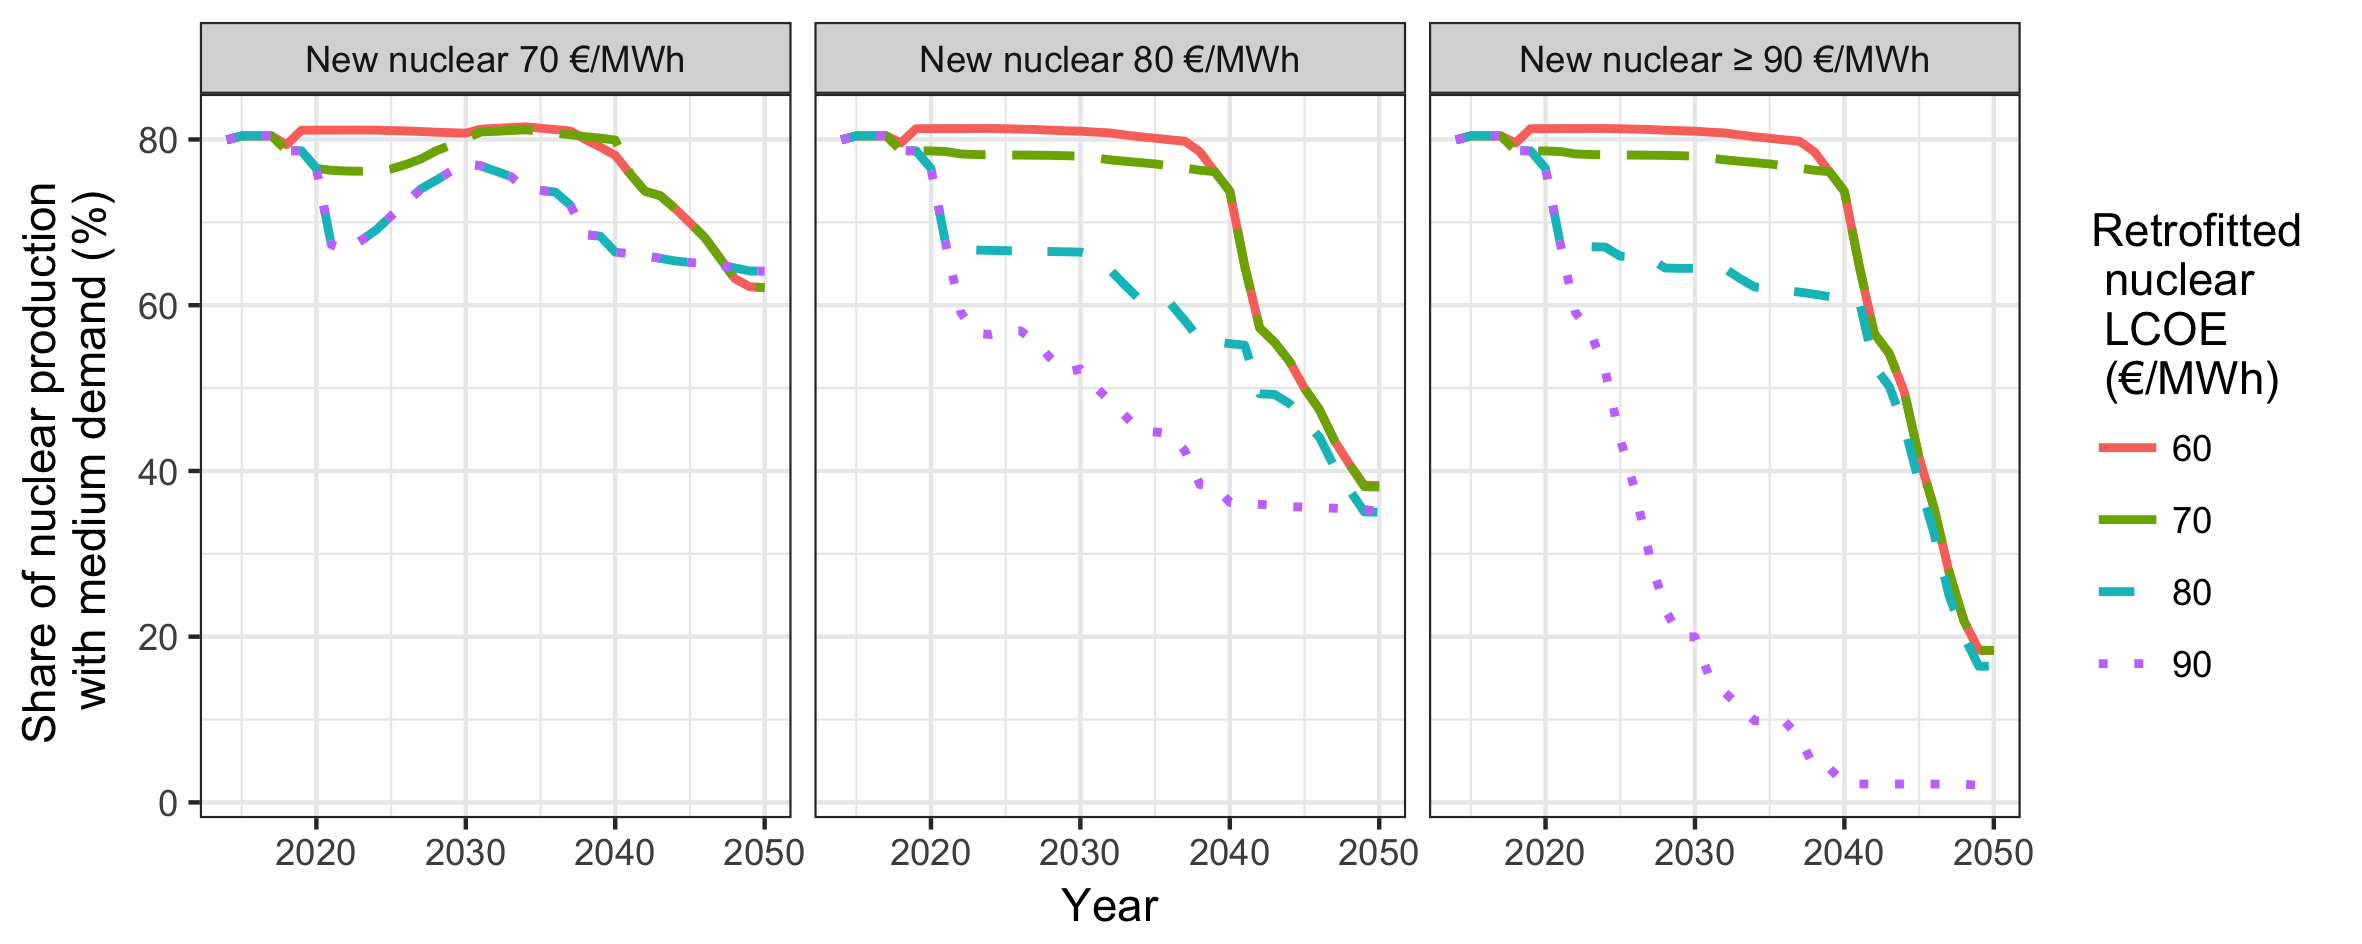
\includegraphics[width=12cm]{figures/nukeShare2_MedD.png}
	\caption{Optimal nuclear share depending on retrofit and new nuclear costs}
	\label{fig:nukeShare}
\end{figure}

From figure \ref{fig:nukeShare} and the sensitivity analysis on demand in figure \ref{fig:powerMixSensitivity}, we can conclude that there is not a single optimum in the range of plausible values. On the contrary, the optimal trajectory depends on several uncertain parameters, in particular the production cost of retrofitted nuclear and demand level. Hence, in this case, the framework of cost-minimization and sensitivity analysis does not allow to conclude to a single trajectory. Following our discussion in section \ref{sec:method}, this motivates the use of the Robust Decision Making framework developed by \citet{Lempert2006}. We now apply it to find robust strategies, and to highlight the potential trade-offs between various robust strategies.

\subsection{Determine plausible future states}

This first step derives from the litterature review in section \ref{sec:plausibleValues}. 
For retrofitted nuclear, we consider that plausible costs range from 40 \emwh\ to 90 \emwh, by step of 10 \emwh. Again, the idea is to encompass a broad initial range in order not to miss any possible value, and the RDM analysis will later identify subsets of costs to draw conclusions. 
As to new nuclear costs, we consider a range from 70 \emwh\ to 110 \emwh, by steps of 20 \emwh. Existing data suggests the cost could be even higher, but since nuclear is not competitive at 110\emwh\ or above in our model, we stop the analysis at this value as it would not add any new information.
For demand, we consider three trajectories drawn from the national debate on energy transition (DNTE): a low, a medium and a high trajectory. They corresponding respectively to the SOB, DIV and DEC scenario, as shown in figure \ref{fig:DNTE_scenarios}.
Finally, we examine two \coo\ price trajectories: a high trajectory using the official price trajectory from \citet{Quinet2009}, and a low trajectory in which this price is divided by two.
Multiplied by the 27 strategies presented in the next section, these parameter ranges require to run the model 2,916 times. 

These parameters were chosen to study the competitiveness of retrofitted and new nuclear plants. What determines the power mix in our model is the relative competitiveness of nuclear compared to gas and renewables. What matters is not their absolute costs, but their relative costs.
Studying a wide range of costs for nuclear is equivalent to studying a wide cost ratio for nuclear and renewables.
Thus, we choose not to include an additional uncertain input for renewable costs. By doing so, we acknowledge that all results in terms of nuclear costs must be linked to our cost assumptions about renewable power sources, and interpreted in terms of cost ratios.


\subsection{Define a set of strategies}

The second step is to define trajectories of nuclear retrofit. The 58 reactors offer 2\textsuperscript{58}=2.9*$10^{17}$ possibilities. As we aim to test each candidate strategy against multiple values of uncertain parameters, this problem is too computationally intensive. Thus, we simplify it by using a smaller sample of strategies. This sample should represent a variability in the number (or share) of retrofitted reactors, and a variability in the time-dimension as it might be more interesting to retrofit at the beginning (e.g. due higher renewable costs), or at the end (e.g. due to higher \coo\ price).

In order to account for the time-dimension, we split the reactors into three groups, according to the end of their initial 40-year lifetime. The first group includes of all reactors which will reach 40 years before 2021, which means the 14 oldest reactors. The second group includes all reactors reaching 40 years between 2021 and 2025, or 23 reactors. The last group includes the 21 remaining reactors. This split enables to explore whether an early retrofit (or phase-out) should be preferred over a late retrofit (or phase-out). 

To account for the variability in the share of retrofit, we consider three possibilities for each group: i) all reactors are retrofitted; ii) half of the reactors are retrofitted (refurbishing every other reactor from oldest to newest in the group) and iii) no reactor is retrofitted. We end up with 3\textsuperscript{3}=27 different strategies. 
More information on these 27 strategies can be found in appendix \ref{sec:strategies_examined}. Our aim will be to find which of these strategies are robust, performing well in a wide range of futures. 

From a policy point of view, it is important to define now a strategy for the medium-term and even long-term, because investment in retrofitting must be made months or years in advance. It can even be ten years in advance, as the decennial stop related to the mandatory safety check is a good opportunity to start a retrofit. 
This implies that the future of the oldest nuclear plants, starting with Fessenheim, must be decided soon. 
Proposing long-term robust strategies would contribute to the current public debate in France about the decommissioning of this plant, and about the amount of compensations to EDF if the plant were to be closed by a public decision.
In the future, as new information becomes available regarding costs, demand, \coo\ price or any other important parameter, the analysis should be re-runned in an iterative and flexible process.

\subsection{Identify candidate strategies}

The following step is to choose a candidate strategy $s_{candidate}$ that performs well across all futures. Our indicator of performance is the upper-quartile regret. This upper-quartile regret is also the indicator used by \citet{Lempert2006} and \citet{Nahmmacher2016} to pick a candidate strategy. The idea of this indicator is to select a strategy that is not too far from the optimum in 75\% of the cases, i.e. that performs well in most cases -- and we will explore remaining 25\% later by analyzing the vulnerabilities of our candidate strategy. 

Using the costs resulting from our model runs, we compute for each strategy $s \in \mathbb{S}$ its regret in each future state $f \in \mathbb{F}$. Then we compute the upper-quartile regret for each strategy $s$. The results are shown in figure \ref{fig:regret}. Each dot in the figure shows the regret, in percent, for a strategy $s$ indicated on the x-axis, and a future $f$. The upper-quartile regret is represented by the larger dots. This figure shows that strategy S9 is a good candidate strategy, as it has the lowest upper-quartile regret (3.9\%). S9 is a strategy in which no plant is retrofitted up to 2021 -- which represents an early phase-out for 14 reactors -- but then all other plants are retrofitted.

But figure \ref{fig:regret} also shows that the strategies S18 and S24 are not far from S9 in terms of regret. Their upper-quartile regret is 4.5\% and 4.2\% respectively. 
S24 is a strategy in which all reactors are retrofitted in the first and third period, but only half of them in the second period. S18 is a strategy in which half the reactors are retrofitted in the first period, and then all of them are retrofitted.
In his paper, \citet{Lempert2006} go on with the RDM analysis considering just one candidate strategy, stating that the final results are not sensitive to the choice of the initial candidate strategy. However, given how close S9, S18 and S24 are in terms of upper-quartile regret, we will perform the rest of the analysis using these three strategies as candidates, in order to make sure our results are not sensitive to the choice of the candidate strategy (S9 is our main candidate strategy, for which will display the figures in the paper, but similar figures for S18 and S24 will be available in the appendix).

\begin{figure}[!ht]
	\centering
	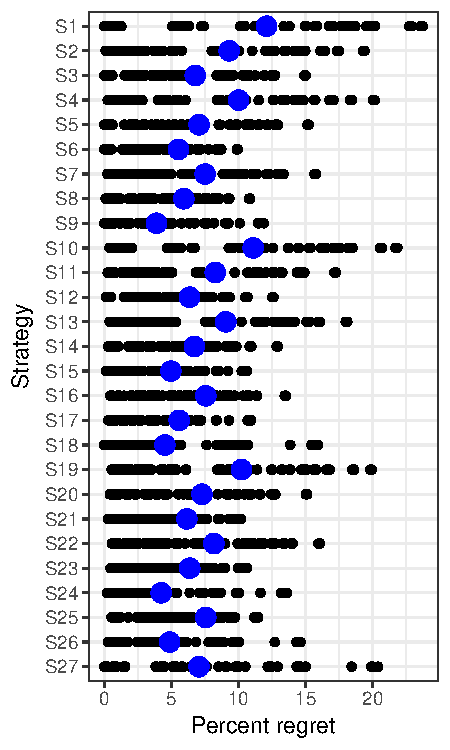
\includegraphics[height=7cm]{figures/regret.pdf}
	\caption{Regret of 27 strategies over 108 plausible states of future}
	\label{fig:regret}
\end{figure}

\subsection{Identify vulnerabilities}

To identify the vulnerabilities of the candidate strategies, we use the Patient Rule Induction Method (PRIM), originally developed by \citet{Friedman1999}. This PRIM algorithm helps identify subsets of parameters in which our target indicator (regret) is above a defined threshold. Documentation on PRIM's operation can be found in \citet{Bryant2010}. We use a public version of the PRIM algorithm implemented in Python in the package called "prim" \citep{Hadka}. 

A regret threshold must be defined to use this PRIM analysis. The ordered distribution of regret shows that regret increases strongly above the threshold 5\% for each candidate strategy S9, S18 and S24 (cf. figure \ref{fig:quantile_regret}). This value of 5\% corresponds to the 80th centile for S18 and S24, and to the 83th centile for S9, which is close to the upper-quartile regret threshold used by \citet{Nahmmacher2016}. Thus, we choose this value of 5\% as a threshold. 

The PRIM algorithm that, for strategy S9, the most common pattern associated with a regret above 5\% is when retrofit costs is equal to or greater than 80 \emwh in conjunction with a low demand level. These two conditions provide a cluster of states of future $\mathbb{F}_{vuln}(S9)$ to which S9 is vulnerable. Since the states of future in the PRIM-generated clusters do not play in favour of nuclear competitiveness, so we call them "retrofit adverse" states. By opposition, we will call "retrofit friendly" states the remaining states in $\mathbb{F}_{rob}(S9) = \mathbb{F} - \mathbb{F}_{vuln}(S9)$.  

Applying PRIM to strategies S24 and S18 shows that the most common pattern associated with a regret above 5\% is the same for these two strategies: when retrofit costs is equal to or greater than 80 \emwh\ in conjunction with a low \coo\ price and a low to medium demand level. This provides another cluster of "retrofit adverse" states.


\subsection{Characterize trade-offs among strategies}

Identifying vulnerabilities enables us to characterize trade-offs between different strategies. Figure \ref{fig:low_regret_frontier_S9} compares the upper-quartile regret values for each of the 27 strategies over the two subsets of future states yielded by the PRIM analysis of S9: $\mathbb{F}_{vuln}(S9)$ and $\mathbb{F}_{rob}(S9)$. (The figure with the clusters from S18 and S24 is similar and shown in figure \ref{fig_app:low_regret_frontier} in appendix).
By switching from one strategy to another, it is possible to lower the regret in one cluster of states, but at the expense of increasing the regret in the other cluster of states. For example, switching from S1 to S10 reduces the regret in "retrofit friendly" states, but increases the regret in "retrofit adverse" states. 
A decision maker can use this figure to choose a strategy that offers the trade-off he prefers. 

From S1 in the upper-left corner to S18 in the bottom-right corner, there is a continuum of available strategies. 
However, some strategies offer a better trade-off than others. 
These strategies are labelled in black. From left to right in the figure, these are S1, S12, S6, S9 and S18. 
They are all located on what can be called a low-regret frontier. 
Some other interesting strategies (though not on the low-regret frontier) are shown in light grey. 
S27 is important as it is the strategy of full retrofit, a policy option often prompted in the public debate. 
It appears that this strategy is far from the low-regret frontier. 
This is due to its vulnerability to a low demand (see figure \ref{fig_app:vulnerabilities_S27} in the appendix). In other words, retrofitting all existing nuclear plants might lead to a costly overcapacity.

Evidencing this low-regret frontier is an important result, because it enables to select only five strategies as potential robust candidates out of the 27 initial strategies examined. This narrowed choice provides a simpler picture of our initial problem, showing only the strategies with interesting trade-offs.

\begin{figure}[!ht]
	\centering
	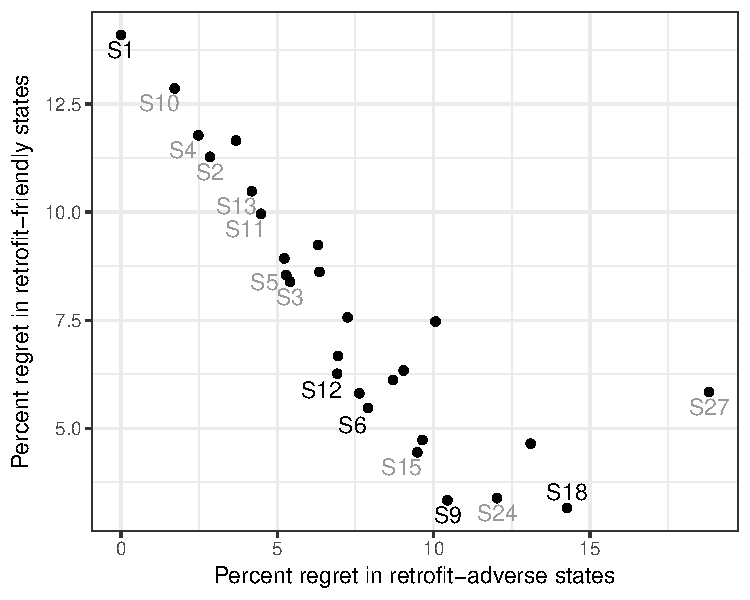
\includegraphics[width=8cm]{figures/low_regret_frontier_S9.pdf}
	\caption{Regret for each strategy in each subset identified}
	\label{fig:low_regret_frontier_S9}
\end{figure}

Having identified the strategies located on the low-regret frontier, the choice of a decision-maker will ultimately depend on his implicit probabilities that a retrofit friendly state occurs. 
This is particularly true for nuclear, which is a controversial source of power, and for which a vast array of costs is plausible. 
If the decision-maker thinks the retrofit friendly cluster is not likely, he will choose to go for S1, the full phase-out strategy; if, on the contrary, he believes the odds of a retrofit friendly state are high, he will pick S18. 

We can simplify the low-regret frontier representation to highlight the most interesting trade-offs between strategy. To that end, we compute the expected regret of a strategy, depending on the relative odds of the two clusters. This is done in figure \ref{fig:odds_S9} for the clusters from strategy S9. This figure shows that there are four main options which can claim to be optimal, depending on the implicit probabilities of the decision maker. 
The x-axis shows the odds of the "retrofit adverse" states versus the odds of the "retrofit friendly" states. 
The y-axis shows the regret associated with each strategy and implicit odds. 
The target of a decision-maker is to pick a strategy with the lowest regret. 
If he believes that a retrofit friendly state is unlikely (odds below 1:1), he should pick strategy S1. 
On the contrary, if he believes that a retrofit friendly" state is certain, he should pick strategy S18.
If he believes that a retrofit friendly state is more likely but not certain, he should pick strategy S9.
Finally, there is a case in which strategy S12 would be picked: if the decision maker thinks the odds are very close to 1:1.
If we use the PRIM-generated clusters based on strategy S18 and S24, the results are similar, except that strategy S12 is replaced with strategy S6. This is shown in figure \ref{fig_app:odds} in the appendix.


\begin{figure}[!ht]
	\centering
	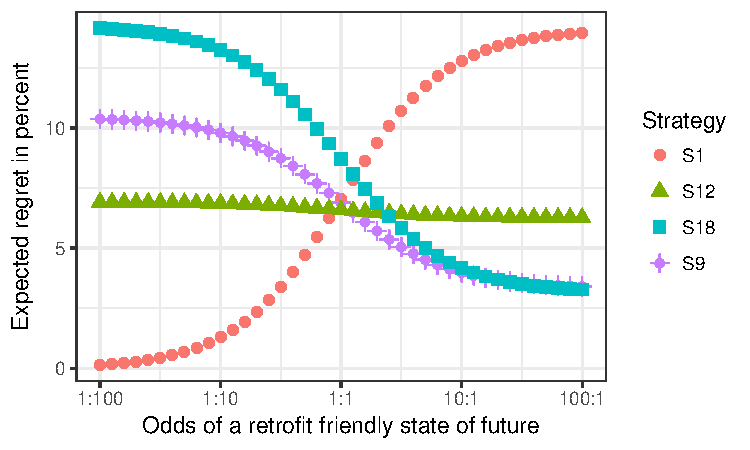
\includegraphics[width=8cm]{figures/odds_S9.pdf}
	\caption{Expected regret of low-regret strategies depending on the implicit probabilities of a decision maker}
	\label{fig:odds_S9}
\end{figure}

The results shown in figure \ref{fig:odds_S9} do not try to settle the debate on nuclear. On the contrary, they show that various strategies can be considered as optimal from a cost-minimization perspective. This helps understand the coexistence of various opinions. But they also provide a quantified framework which accounts for uncertainty to support policy decision. 

Currently, the cost of retrofitted nuclear is estimated at around 40 \emwh\ by EDF. Although there is a lot of uncertainty about that figure, a cost of retrofitted nuclear below 80 \emwh\ seems more likely today. Thus, strategies S9 and S18 seem to be the best robust strategies given current cost estimates, in the sense that they yield the lowest expected regret over a large range of the most plausible future states.

S9 and S18 are close strategies: they are both based on a full retrofit after 2021. The difference is that S18 include to retrofit 50\% of the 14 oldest plants, while S9 plans to retrofit none. 
Both strategies yield the lowest regret in the most likely future states, as shown in \ref{fig:low_regret_frontier_S9}, providing a good hedge against higher than expected cost of nuclear, low demand of low carbon price. 
Choosing between S9 and S18 will be a matter of implicit probability of the decision maker. S18 is slightly more performing if nuclear is below 60 \emwh and demand is flat or increasing. But S9 performs better if demand is low, and it is less vulnerable to an increase in retrofit costs in conjunction with a low \coo\ price (cf. figure \ref{fig_app:vulnerabilities_S9_S18_S27} in appendix).

In conclusion, we have evidenced that the most robust strategies imply an early-phase out of 7 to 14 out of the 14 oldest reactors, given the current estimates of cost, demand and \coo\ price. The intuition behind these results comes from a balance between risks and costs. On one hand, retrofitting all plants is a strategy vulnerable to lower demand or higher than expected costs of retrofit. On the other hand, nuclear provides a low-carbon, flexible source of electricity. Higher share of renewables entails a drop in the value of their production, due to autocorrelation and increasing flexibility burden for the system. This reduces their competitiveness as their penetration rate increases. Our analysis has revealed two robust strategies in-between these two extremes, which imply closing 7 to 14 reactors. 
We also highlighted their vulnerabilities, their alternatives, and the potential trade-offs with other strategies. Our approach keeps the debate open, as we highlight that other strategies might be considered cost-optimal for assumptions less in line with the literature, but still plausible given the current uncertainty. 
The final choice of a strategy will ultimately depend on the implicit probabilities perceived by the decision-maker. We thus contribute to the debate on nuclear in France, in particular with respect to the retrofit of the nuclear plants of Fessenheim and Bugey, which will reach 40 years in 2017 and 2018 respectively.


%%%%%%%%%%%%%%%%%%

\section{Comparison with French official scenarios}
\label{sec:comparison}

\subsection{Presentation of the official scenarios}

From 2012 to 2015, France engaged in a National Debate on the Energy Transition (\dnte), which finally led to a new "Law on the Energy Transition for a Green Growth"\footnote{
	Loi 2015-992 du 17 août 2015 relative à la transition énergétique pour la croissance verte.
}.
A discussion on the future of the energy mix brought together various political stakeholders, as well as unions and NGOs.
During the debate, the power mix and the share of nuclear were a point of particular focus, with a dedicated working group. Eleven energy transition scenarios were created by the different parties to promote their own vision of France's energy landscape, and these scenarios were ultimately grouped into four representative scenarios.

These four scenarios represent the different views that existed in 2012, and they have been structuring the French debate on nuclear ever since. The rationale of each representative scenario is summarized in table \ref{tab:dnteScenarios}, but more information can be found in \citet{DNTE_gt2}.
Quantitatively, each scenario can be defined by two criteria: demand level and nuclear share, as detailed in figure \ref{fig:DNTE_scenarios}.

\begin{table}
	%\colorTable
	\begin{tabular}{p{2cm}p{6cm}cp{2.5cm}}
		\toprule
		Scenario name & Scenario description & Demand & Nuclear Share \\
		\midrule
		Sobriety (SOB)     	& A strong energy efficiency and sobriety reduce power demand.\newline Nuclear and fossil fuels are phased out. & Strong decrease & Full phase-out \\
		Efficiency (EFF)  	 & Ambitious energy efficiency targets and diversification of power sources & Slight decrease & Decrease to 50\% in 2030 and 25\% in 2040 \\
		Diversification (DIV) 	& Diversification of power sources & Slight increase & Decrease to 50\% from 2030 onwards \\
		Decarbonation (DEC)  & High power demand due to increase electrification and high nuclear share & Strong increase & Full retrofit \\
		\bottomrule
	\end{tabular}
	\caption{\label{tab:dnteScenarios}DNTE scenarios}
\end{table}


\subsection{Robust vs official scenarios}
Based on these criteria of demand level and nuclear share, we can find which strategy among the 27 studied in this paper would best represent each official scenario. 
The DEC scenario corresponds to a retrofit of all nuclear plants. The SOB scenario is a scenario of full phase-out. Thus, their equivalent strategies are S27 and S1 respectively. But a methodology is required to determine the equivalent strategy of the EFF and DIV scenarios. 
To that end, we combine the information on nuclear share and demand level in each scenario to deduct the annual nuclear power generation in 2020, 2030 and 2040.
Generation is used as a proxy to estimate the number of retrofitted plants (it is a better proxy than nuclear share, as it accounts for the differences in demand level between the four scenarios of the DNTE). Based on the three years 2020, 2030 and 2040, we compute the distance between the nuclear production in each strategy and the nuclear production in the DNTE scenarios. Distance $D$ is defined here as the square root of the sum of squared difference in nuclear production for each year:
$$D(\text{strategy, DNTE scenario}) = \sqrt{ \sum_{\text{y in {2020,2030,2040}}} (Prod^y_{\text{strategy}} - Prod^y_{\text{scenario DNTE}})^2}$$
where $Prod^y$ is the production in year $y$.
With this methodology, the best matches for the EFF and DIV scenarios are S13 and S6 respectively. In addition, this distance-based methodology gives respectively S1 and S27 as best estimates for the SOB and DEC scenarios, as expected.

Now that we have identified which strategy matches each scenario of the DNTE, we can build on our previous analysis. Figure \ref{fig:low_regret_frontier_S9} shows that the four DNTE scenarios (S1, S13, S6, S27) cover well the spectrum of possible trade-offs: S1 and S27 are the two extreme points of full phase-out and full retrofit respectively. S13 and S6 provide more balanced intermediate points, with a retrofit share of 27\% and 63\% respectively. Thus, the DNTE scenarios offers a representative panel of the policy options available in terms of capacity decommissioned.

However, our RDM analysis has also revealed the shortcomings of the DNTE scenarios and the contribution of our RDM analysis. 
First, we showed that the full-retrofit option, DEC (S27), is not a low-regret option. This is due to its high vulnerability to a decreasing demand. This is an important result because the full retrofit is often presented as the cheapest policy option in the public debate.
Second, we explored 27 strategies instead of just four scenarios, and we highlighted their trade-offs given implicit assumptions about the future cost of nuclear. 
Results from a pure cost-minimization framework can only state what is the optimal power mix given a fixed set of assumptions on costs, demand, \coo\ price, etc. But since there is uncertainty on these parameters, the message is not easily transformed into a policy advise.

With RDM analysis, we simplified a multidimensional problem to a simple trade-off between two possible clusters of future states. We show the trade-offs in terms of implicit probabilities, providing a message more readable and easier to use by decision makers: "if you think a retrofit friendly state is likely, you should aim for S9; if you think it is certain, pick S18; if you think it is unlikely, pick S1". 
Finally, we showed that two strategies in particular, S9 and S18, are likely to provide the lowest regret --given current cost estimates-- over a large range of the most plausible future states. These robust strategies consist in decommissioning 7 to 14 of the 14 oldest reactors, and then retrofit all the remaining ones. These are two intermediate paths that were missing in the four official scenarios. Currently, the options were either to retrofit all plants or close more than 30 reactors. Thus, we have evidenced two new robust strategies. This could contribute to the public debate in France, and in other countries where the decision to retrofit or decommission nuclear power plants is discussed.

%%%%%%%%%%%%%%%%%%



\section{Conclusion}
\label{sec:conclusion2}

After the first oil shock, France launched the world’s largest nuclear program, ordering 36 reactors within two years, and 58 reactors in total. These reactors are now reaching the end of their technological lifetime. But extending these lifetimes requires an investment up to \euro 100 billion by 2030. 
France is thus at a crossroads and must define a new nuclear policy. The economics of this decision crucially depend on several parameters, in particular the future costs of nuclear (including decommissioning, waste and insurance), demand levels and the social cost of carbon, all of which are subject to significant uncertainty.

In face of all these uncertainties, we apply the framework of Robust Decision Making (RDM) to find a robust strategy indicating which plants should be retrofitted.

Based on nearly 3,000 runs, our analysis revealed two robust strategies, which imply the early-phase out of between 7 and 14 of the 14 oldest reactors. We also assessed the vulnerabilities and alternatives of such a strategy, as well as the potential trade-offs with other strategies. Our approach keeps the debate open: we highlight that several options exist depending on the implicit probabilities of decision-makers. But considering the current estimates of cost, demand and carbon price, the two aforementioned strategies are likely to yield the lowest regret. 

Our policy recommendation differs from the official French government scenarios which stem from the national debate. Our analysis has thus revealed new, robust strategies. It provides a timely contribution to the debate on nuclear in France, in particular with respect to the retrofit of the nuclear plants of Fessenheim, which will reach 40 years in 2017.

Our framework could be used iteratively in the future. Each time the decision to retrofit a nuclear plant has to be made, the same analysis could be run. The advantage would be to benefit from newer information on costs, the level of electricity demand or the social cost of carbon.


\phantomsection
\printbibliography[heading=subbibintoc] % L'option sert à ajouter la biblio à la table des matières
%\addcontentsline{toc}{section}{Appendices} % Pour ajouter à la table des matières
\begin{subappendices}
\section*{Appendix}

\phantomsection % to make sure the clickable link points to the right page
\addcontentsline{toc}{section}{Appendix} % adds this label to the ToC

\subsection{Model documentation}

\subsubsection{Overview}
The French power model FLORE is a dispatch and investment model of the French power mix. It is a partial equilibrium model of the wholesale electricity market, which determines optimal investment and hourly generation.

FLORE minimizes total cost with respect to investment and production under a set of constraints. The model is linear, deterministic, and solved in hourly time step for each year, from 2014 to 2050.

Generation is modelled as twelve distinct technologies: three VRE with zero marginal costs - onshore wind, offshore wind and solar, three fossil-based thermal technologies - coal, combined cycle gas turbine (CCGT), open cycle gas turbine (OCGT), three nuclear technologies (historical nuclear, retrofitted nuclear and new nuclear), and three hydro systems - run-of-river, conventional dams (lakes) and pumped storage. 
Hourly VRE generation is limited by specific generation profiles.
Dispatchable power plants produce whenever the price is above their variable costs, and unless they are limited by their ramping constraints.
Hydro storage and dispatch is optimized by the model, under water reservoir constraints and pumping losses.
At the end its lifetime, each capacity is decommissioned.

A particularity of the model is to represent explicitly the cost of extending the lifetime of nuclear power plants. Nuclear plants normally close after 40 years, but their lifetime can be extended to 60 years, if upgrade costs are paid for.

Demand is exogenous and assumed to be perfectly price inelastic at all times.

FLORE is currently calibrated for France. Exports are given exogenously.

\subsubsection{Total System Costs}

The model minimizes total system costs $C$ with respect to several constraints and decision variables. Total system costs are the sum of fixed costs (representing the sum of capital and fixed O\&M costs), and variable costs, over all hours $h$, weeks $w$, years $y$ and generation technologies $tec$. 

Fixed costs are the product of the capacity installed $CAPA_{tec,y}$ for each technology in year $y$, by its annualized capacity cost $c_{tec}^{inv}$ plus fixed O\&M costs $c_{tec}^{qfix}$. 
Variable generation costs are the product of $GENE_{tec,w,y,h}$, the generation from technology $tec$ in year $y$, week $w$ and hour $h$, by variable generation costs $c_{tec}^{var}$.
\begin{equation}
C =\sum_{tec,y} CAPA_{tec,y} \cdot ( c_{tec}^{inv} + c_{tec}^{qfix} ) + \sum_{tec,y,w,h} GENE_{tec,y,w,h} \cdot c_{tec}^{var}
\end{equation}
Throughout this model description, capital letters denote choice variable for the model, while lowercase letters denote exogenous data.

\subsubsection{Supply and demand}

Power balance between supply and demand is the central constraint of the model. Demand is the sum of national load $d$, pumping for pumped-storage hydro $PUMP$ and exports flow $flows$. 
Supply is the sum of generation over all technologies.
$$\forall h,y \quad \sum_{tec} GENE(tec,h,y) \geq \sum_{tec} LOAD(h,y) + PUMP(h,y) + flow(h,y)$$

In this framework, demand is perfectly price-inelastic. Cost minimization is thus equivalent to welfare-maximization.

Generation is constrained by capacities installed and the load factor (also called availability), for all technologies except wind, PV and run-of-river hydro, which present a specific generation profile.
$$GENE(tec\_noprof,y,w,h) \leq CAPA(tec\_noprof,y)*loadfactor(tec\_noprof)$$
For wind and PV, a generation profile is an additional constraint:
$$GENE(tec\_res,y,w,h) \leq CAPA(tec\_res,y)*res\_profiles(h,tec\_res)$$
For run-of-river hydro, generation is fixed exogenously for each week:
$$GENE("river",y,w,h) = river\_flow(w)$$

Investment is exogenous for historical nuclear and the three hydro technologies. The capacity of historical nuclear technology is decreasing based on plant-level data, with each plant capacity being phased-out when it reaches 40 years old. For hydro, we assume constant capacities for run-of-river and lakes. Pumped-hydro potential is expected to grow by 3.2GW by 2050, starting from 5 GW in 2014, with a discharge time of 20 hours, as in ADEME (Visions ADEME 2030).
$$CAPA_{tec\_ex,y} = capa_exo_{y,tec\_ex} $$

The capacity of all other technologies is determined endogenously by the model. Capacity is installed when optimal, and then decommissioned when it reaches its lifetime. The initial capacity, already installed in 2014, is supposed to be decommissioned linearly from 2014 onwards in a period of 40 years.
\begin{align*}
CAPA_{tec\_end,y+1} &= CAPA_{tec\_end,y} + INVE_{tec\_end,y} - DECO\_{tec\_end,y} \\
DECO_{tec\_end,y}  &= INVE_{tec\_end,y-lifetime(tec\_end)} + (tec\_data_{tec\_end,'initcap'}/40)\$(ord(y) <= 40) 
\end{align*}



\subsubsection{Power System Inflexibilities}

The model includes ramp-up and ramp-down constraints for nuclear and coal power plants, to represent the fact that generation cannot vary too quickly from one hour to the next. These constraints are modelled as a maximum variation rate:
The ramp up constraint is:
$$\forall tec\_ramp,y,w,h \quad GENE(tec\_ramp,y,w,h+1) \leq GENE(tec\_ramp;y;w;h) \dot (1+ramp\_rate)$$
The ramp-down constraint is:
$$\forall tec\_ramp,y,w,h \quad GENE(tec\_ramp,y,w,h+1) \geq GENE(tec\_ramp;y;w;h) \dot (1-ramp\_rate)$$
We take the value of $0.08$ for coal and $0.05$ for nuclear - for both ramp-up and ramp-down, as in \citet{ADEME2015}.

\subsubsection{Model limitation}

This model was design to model the French power system from 2014 to 2050, optimizing investment and dispatch over many assumptions on nuclear costs. As such, it had to make several simplifying assumptions.

This model does not provide a detailed representation of infra-hourly events. In particular, ancillary services are not represented. 

We do not model power plants at the plant level, but we rather use representative technologies. Thus, one limitation is the absence of constraints related to unit commitment, such as start-up cost and delay, minimum load, and part-load efficiency. 
However, this default is in part compensated for nuclear. We use real data on age limit (or retirement), so the model retrofits plants whose capacity is in line with plant-level data. On the contrary, new nuclear will be installed continuously, while in reality it composed of discrete power plants with a significant size (1.3 GW for the EPR technology).
For renewable, the representative technology assumption is less of an issue as these technologies are modular, and very small in size. The continuous approach is here a good assumption for costs. However, this approach does not enable one to distinguish the different potentials within a country, both for solar and wind. 

%%%%%%%%%%%%%%%%

\clearpage

\subsubsection{Model Calibration}

\label{app:calibration}

The model is calibrated using capital cost, fixed O\&M and variable O\&M costs. All payments are annualized with a 5\% interest rate. The corresponding LCOE with usual load factor are given in the Figure \ref{fig:calibration_LCOE}.

\begin{figure}[!ht]
	\centering
	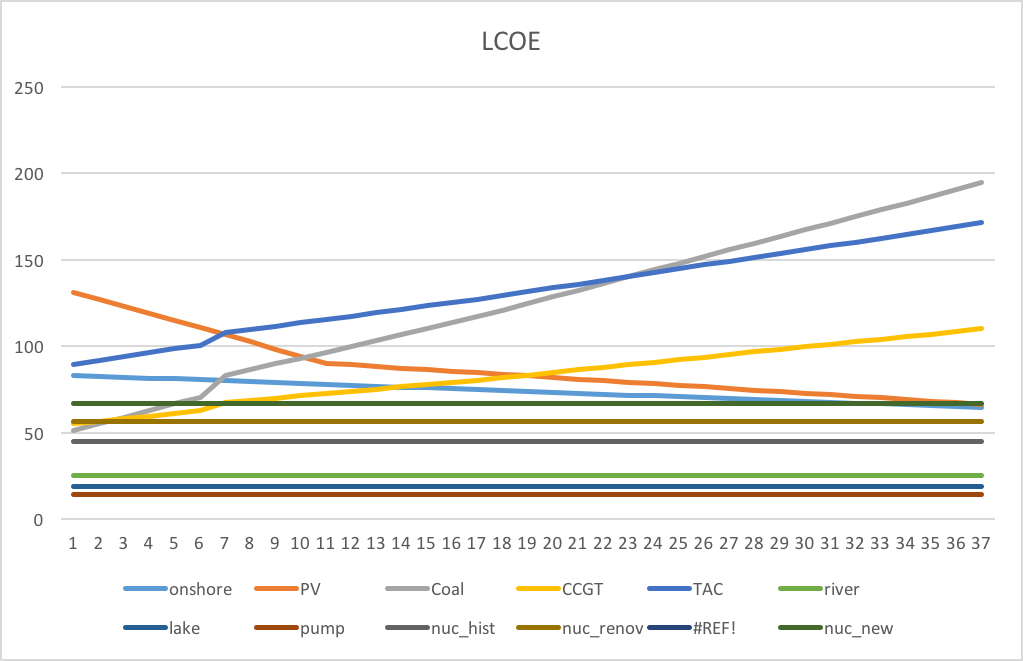
\includegraphics[width=12cm]{figures/calibration_LCOE.png}
	\caption{LCOE utilisés dans le modèle}
	\label{fig:calibration_LCOE}
\end{figure}

\begin{table}[!ht]
	%\colorTable
	\centering
	\caption{Main model parameters}
	\begin{tabular}{llr}
		\toprule
		parameter&value&unit\\
		\midrule
		Rate of pure time preference &0&\%\\
		Financial interest rate&5&\%\\
		\bottomrule
	\end{tabular}
\end{table}

\begin{table}[!ht]
	\centering
	\caption{Investment costs (euros/kW)}
	\label{tab:Investment _costs}
	\begin{adjustbox}{width=1\textwidth}
	\small
	\begin{tabular}{llllllllllll}
		\toprule
		 Year & onshore & PV & Coal & CCGT & TAC & river & lake & pump & nuc\_hist & nuc\_renov & nuc\_new \\
		\midrule
		2014 & 1650 & 1560 & 1500 & 800 & 400 & 3000 & 2000 & 2000 & 1320 & 1938 & 6000 \\
		2020 & 1572 & 1194 & 1500 & 800 & 400 & 3000 & 2000 & 2000 & 1320 & 1938 & 6000 \\
		2030 & 1443 & 869 & 1500 & 800 & 400 & 3000 & 2000 & 2000 & 1320 & 1938 & 6000 \\
		2040 & 1313 & 735 & 1500 & 800 & 400 & 3000 & 2000 & 2000 & 1320 & 1938 & 6000 \\
		2050 & 1184 & 600 & 1500 & 800 & 400 & 3000 & 2000 & 2000 & 1320 & 1938 & 6000 \\
		\bottomrule
	\end{tabular}
\end{adjustbox}
\end{table}

\begin{table}[!ht]
	\centering
	\caption{Fixed O\&M costs (euro/MWh)}
	\label{tab:OM_costs}
		\begin{adjustbox}{width=1\textwidth}
	\small
	\begin{tabular}{llllllllllll}
		\toprule
		Year & onshore & PV & Coal & CCGT & TAC & river & lake & pump & nuc\_hist & nuc\_renov & nuc\_new \\
		\midrule
		2014 & 35 & 25 & 30 & 20 & 15 & 60 & 60 & 20 & 188 & 188 & 100 \\
		2020 & 35 & 25 & 30 & 20 & 15 & 60 & 60 & 20 & 188 & 188 & 100 \\
		2030 & 35 & 25 & 30 & 20 & 15 & 60 & 60 & 20 & 188 & 188 & 100 \\
		2040 & 35 & 25 & 30 & 20 & 15 & 60 & 60 & 20 & 188 & 188 & 100 \\
		2050 & 35 & 25 & 30 & 20 & 15 & 60 & 60 & 20 & 188 & 188 & 100 \\
		\bottomrule
	\end{tabular}
\end{adjustbox}
\end{table}


\begin{table}
	\centering
	\caption{\coo\ price}
	\label{tab:CO2_price}
	\begin{tabular}{llll}
		\toprule
		Year & \coo\ price & & \\
		\midrule
		& Central & Low & High \\
		2014 & 21 & 10 & 42 \\
		2020 & 28 & 14 & 56 \\
		2030 & 50 & 25 & 100 \\
		2040 & 75 & 38 & 150 \\
		2050 & 100 & 50 & 200 \\
		\bottomrule
	\end{tabular}
\end{table}



\begin{table}[!ht]
	\centering
	\caption{Fuel prices}
	\label{tab:Fuel_prices}
	\begin{tabular}{llll}
		\toprule
		euro/MWh & Coal & Gas & Uranium \\
		\midrule
		2014 & 10,3 & 25,3 & 7,30 \\
		\bottomrule
	\end{tabular}
\end{table}

\begin{table}
	\centering
	\caption{Efficiencies}
	\label{tab:Efficiencies}
	\begin{tabular}{lll}
		\toprule
		Coal & CCGT & TAC \\
		\midrule
		0,43 & 0,61 & 0,410 \\
		\bottomrule
	\end{tabular}
\end{table}

%%%%%%%%%%%%%%%%%%
\clearpage
\subsection{Additional material}

\subsubsection{Plausible costs of retrofitted plants}


\begin{table}
	\centering
	\caption{Historical values of French nuclear plants in the literature, in the best case}
	\label{tab:historical_costs}
	\begin{tabular}{llll}
		\toprule
		Item & Cost & Unit & Source \\
		\midrule
		Historical OPEX & 13.3 & euro/MWh & Boccard, 2014 \\
		Fuel & 5.7 & euro/MWh & Cour des Comptes, 2014, p. 13 \\
		Waste & 3.6 &  & Cour des Comptes, 2014, p. 24 \\
		Decommissioning & 1 &  & Cour des Comptes, 2014, p. 24 \\
		Capital rate & 5 & \% &  \\
		Lifetime extension & 20 & years & \\
		availability & 83.5 & \% & \\
		\bottomrule
	\end{tabular}
\end{table}


\begin{table}
	\centering
	\caption{Retrofit costs according to EDF}
	\label{tab:costs_grand_carenage}
	\begin{tabular}{lll}
		\toprule
		Additional CAPEX & 74730 & million euros \\
		\midrule
		Additional OPEX & 25160 & million euros \\
		Capacity concerned & 53200 & MW \\
		\bottomrule
	\end{tabular}
\end{table}


\begin{table}
	\centering
	\caption{Sensitivity tests}
	\label{tab:sensitivity_tests}
	\begin{tabular}{lll}
		\toprule
		CAPEX & 30 & \% \\
		\midrule
		Historical OPEX & 27.5 & euro/MWh \\
		Capital rate & 10 & \% \\
		Lifetime extension & 10 & years \\
		Availability & 70 & \% \\
		Waste & x2 &  \\
		Decommissioning & x2 &  \\
		Insurance & 8.5 & euro/MWh \\
		\bottomrule
	\end{tabular}
\end{table}



\subsubsection{Strategies examined}
\label{sec:strategies_examined}

\begin{figure}[!ht]
	\centering
	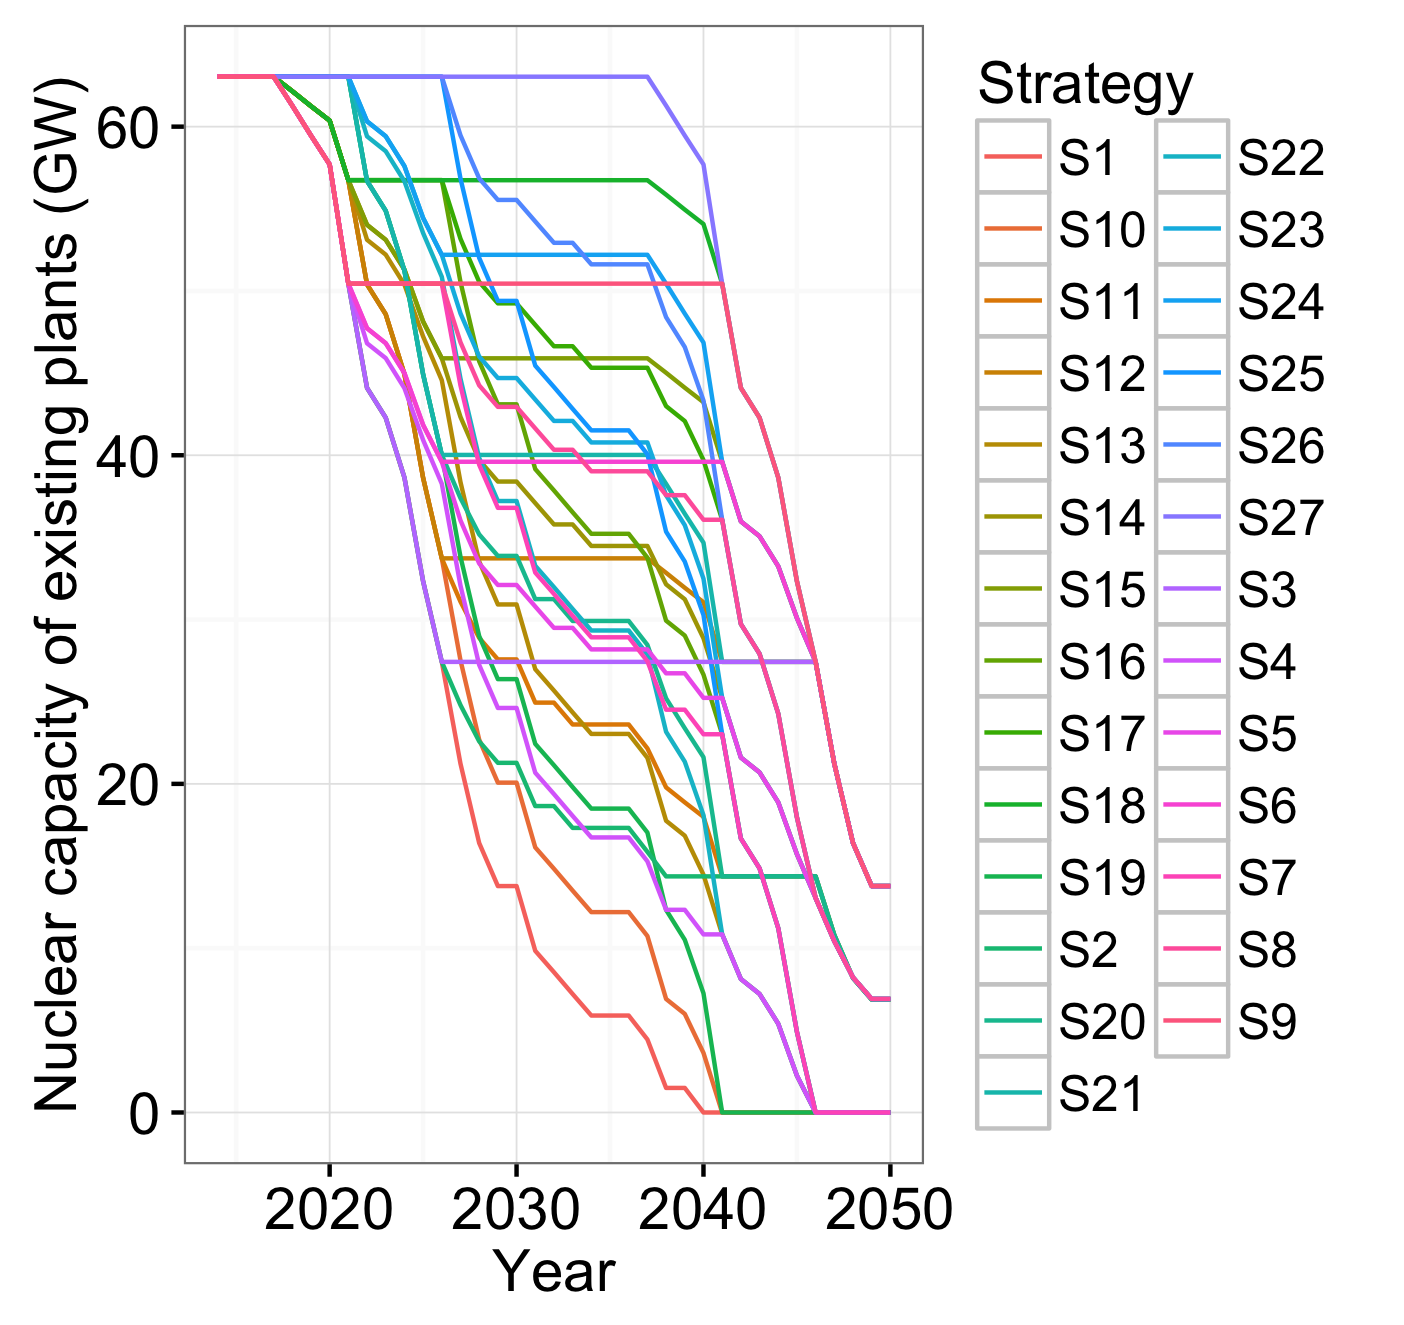
\includegraphics[height=7cm]{figures/strategies.png}
	\caption{Nuclear capacity of existing plants, including retrofit, in the 27 strategies}
	\label{fig:strategies}
\end{figure}

\clearpage

\begin{table}
	\centering
	\caption{Share of retrofitted nuclear plants in each period}
	\label{tab:shareNukeRetrofit}
	\begin{tabular}{llll}
		\toprule
		Strategy & Period1 & Period2 & Period3 \\
		\midrule
		S1 & 0\% & 0\% & 0\% \\
		S2 & 0\% & 0\% & 50\% \\
		S3 & 0\% & 0\% & 100\% \\
		S4 & 0\% & 50\% & 0\% \\
		S5 & 0\% & 50\% & 50\% \\
		S6 & 0\% & 50\% & 100\% \\
		S7 & 0\% & 100\% & 0\% \\
		S8 & 0\% & 100\% & 50\% \\
		S9 & 0\% & 100\% & 100\% \\
		S10 & 50\% & 0\% & 0\% \\
		S11 & 50\% & 0\% & 50\% \\
		S12 & 50\% & 0\% & 100\% \\
		S13 & 50\% & 50\% & 0\% \\
		S14 & 50\% & 50\% & 50\% \\
		S15 & 50\% & 50\% & 100\% \\
		S16 & 50\% & 100\% & 0\% \\
		S17 & 50\% & 100\% & 50\% \\
		S18 & 50\% & 100\% & 100\% \\
		S19 & 100\% & 0\% & 0\% \\
		S20 & 100\% & 0\% & 50\% \\
		S21 & 100\% & 0\% & 100\% \\
		S22 & 100\% & 50\% & 0\% \\
		S23 & 100\% & 50\% & 50\% \\
		S24 & 100\% & 50\% & 100\% \\
		S25 & 100\% & 100\% & 0\% \\
		S26 & 100\% & 100\% & 50\% \\
		S27 & 100\% & 100\% & 100\% \\
		\bottomrule
	\end{tabular}
\end{table}

The first period includes all reactors that reach 40 years before 2021, which represents 14 reactors. The second period includes all the reactors reaching 40 years between 2021 and 2025, which represent 23 addditional reactors. The final period goes up to 2050 and represents the remaining 21 reactors.
\subsubsection{Optimum power mixes}
\label{app:optimumMixes}


\begin{figure}
	\centering
	\subfloat[Optimum for retrofitted nuclear below or equal to 40 \emwh] {
		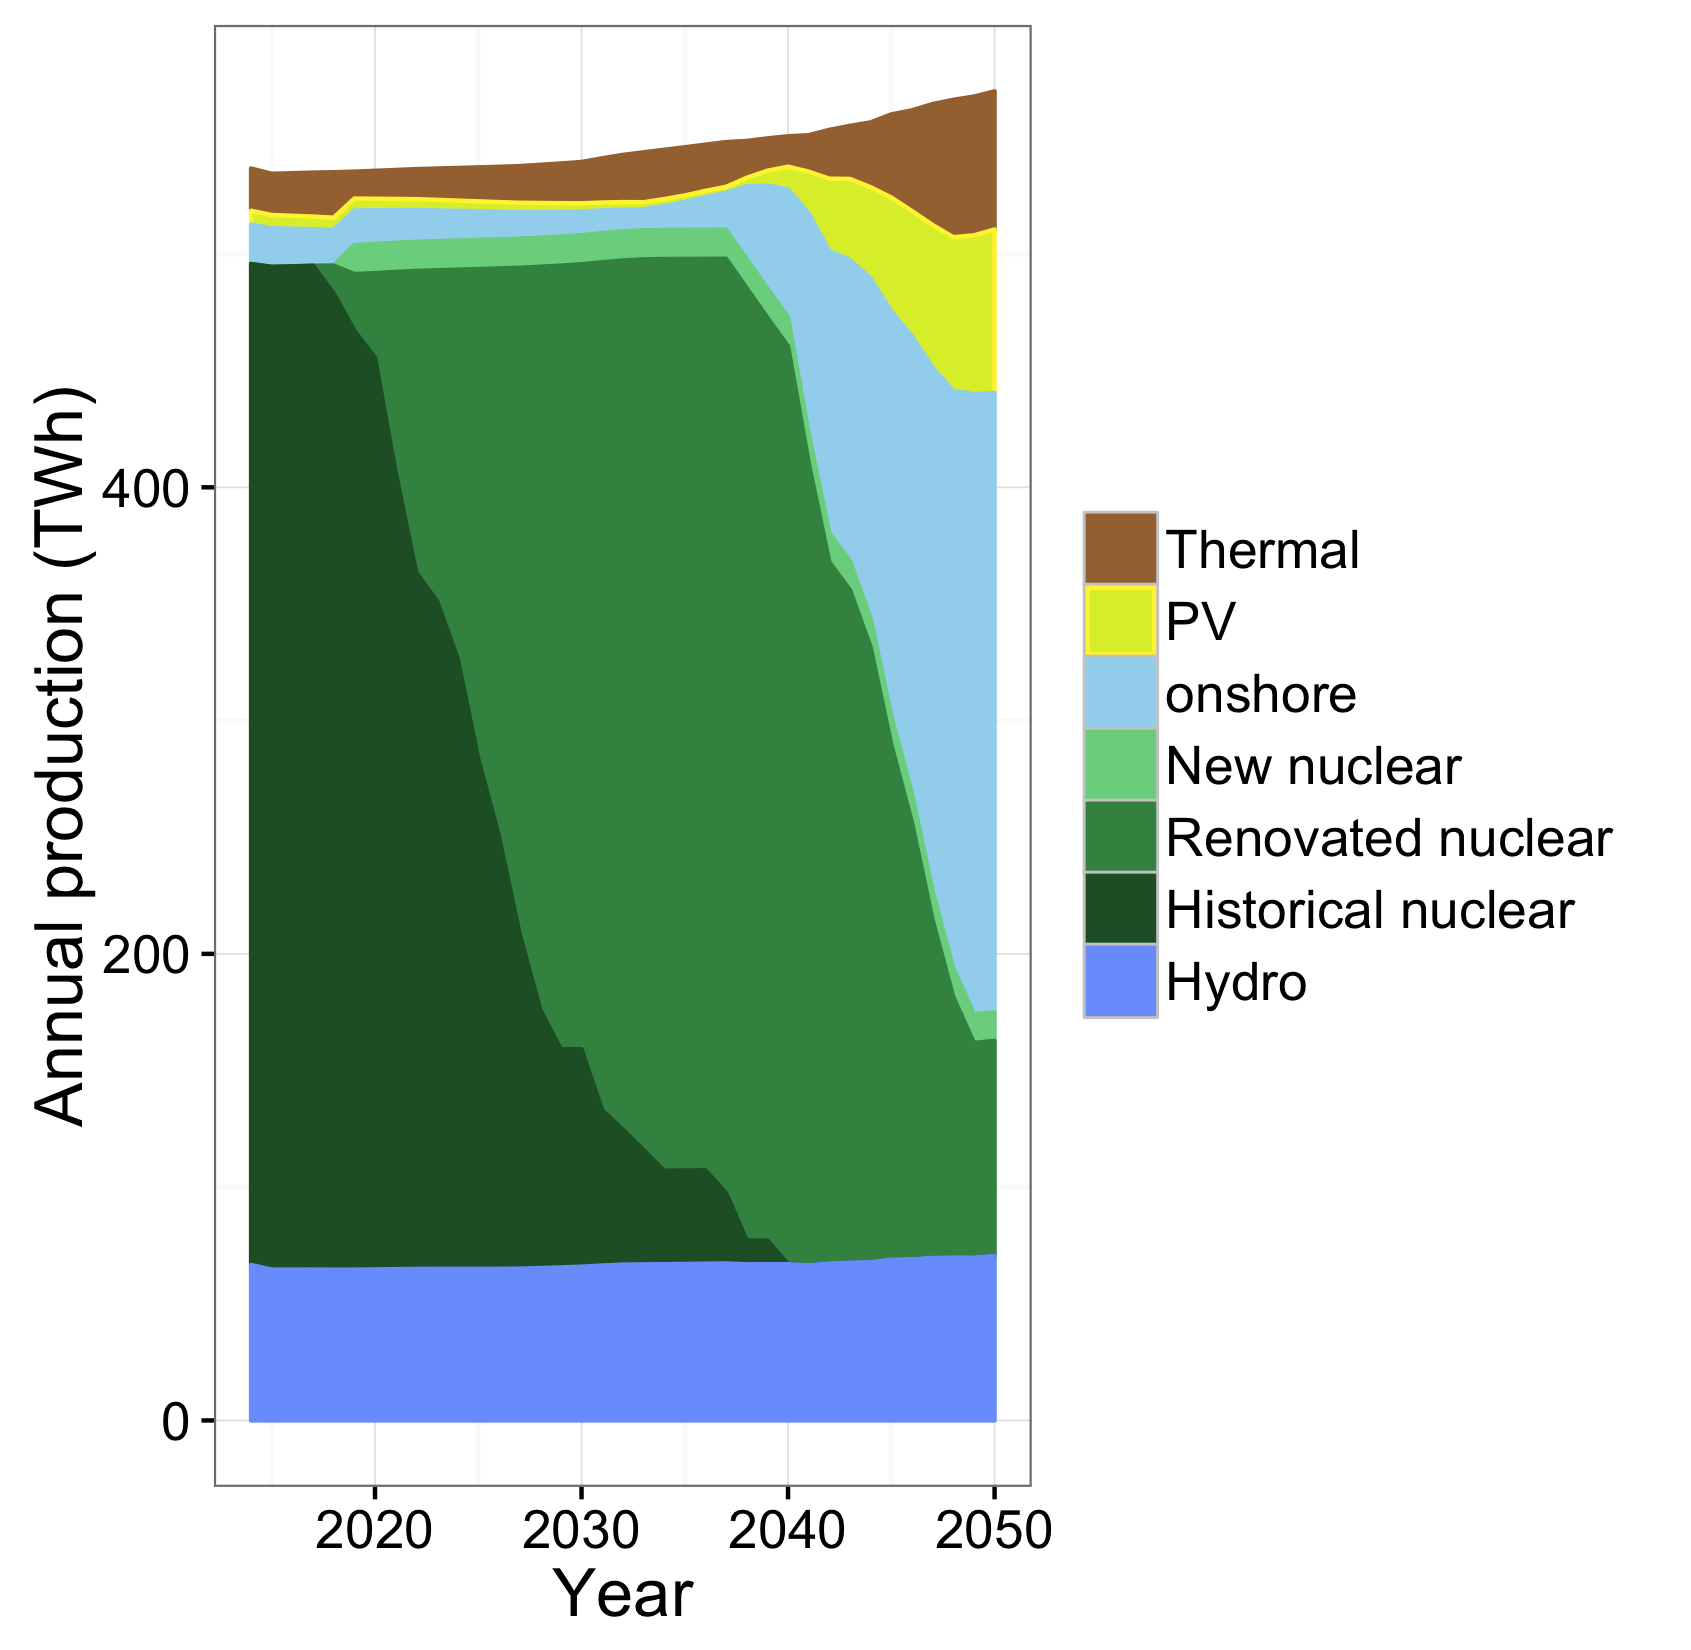
\includegraphics[width=7cm]{figures/powerMix_R40N100MedD.png}
		\label{fig:nukeShare40}
	}
	\subfloat[Optimum for retrofitted nuclear around 70 \emwh] {
		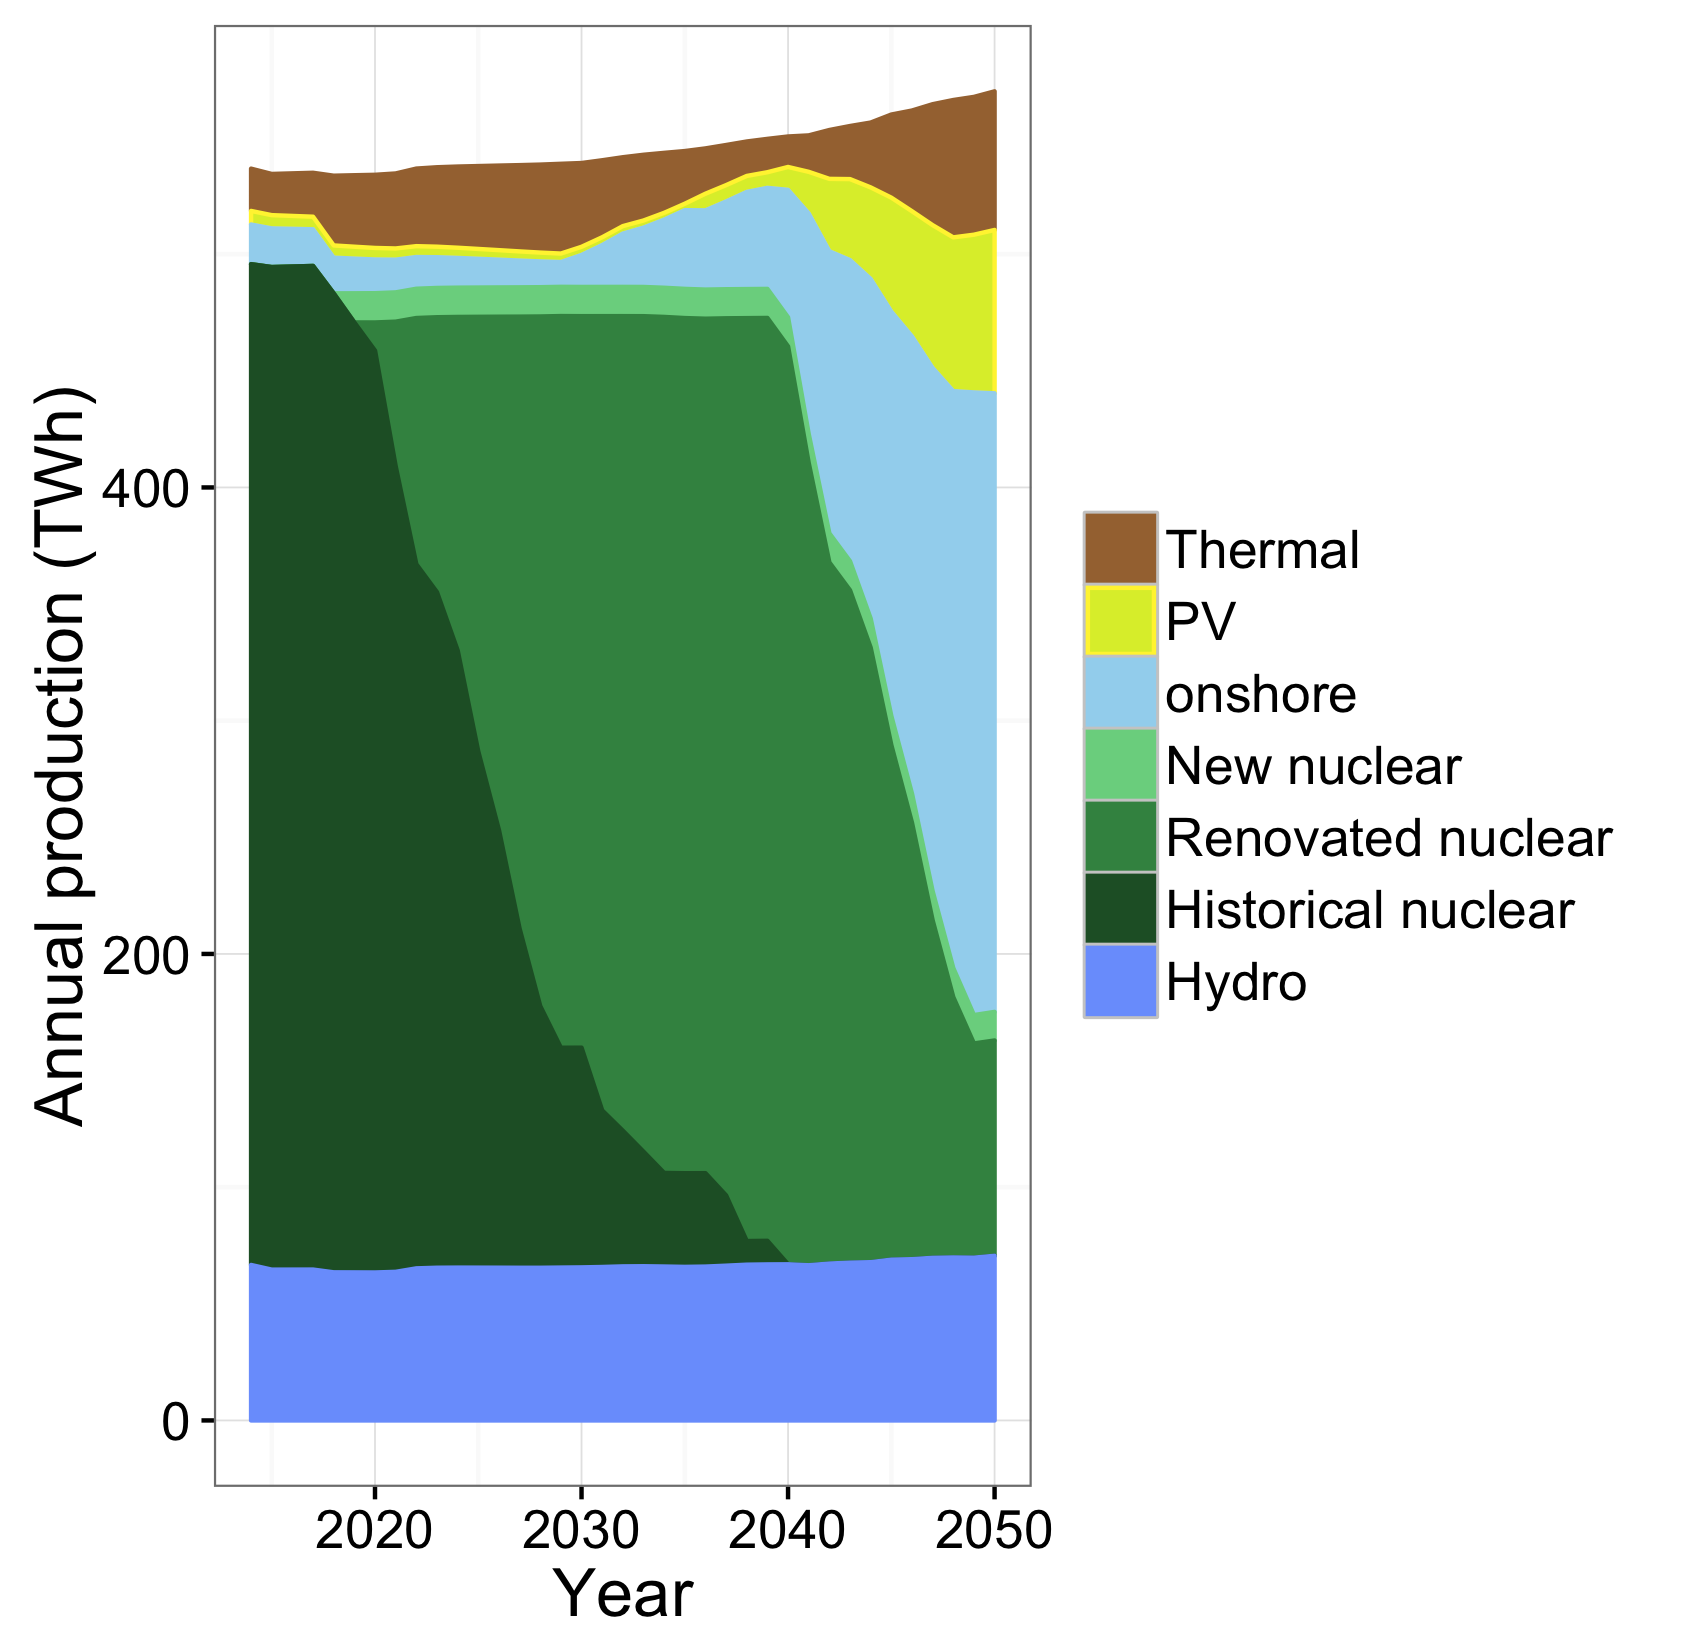
\includegraphics[width=7cm]{figures/powerMix_R70N100MedD.png}
		\label{fig:nukeShare70}
	}
\end{figure}

\begin{figure}
	\centering
		\subfloat[Optimum for retrofitted nuclear around 80 \emwh] {
		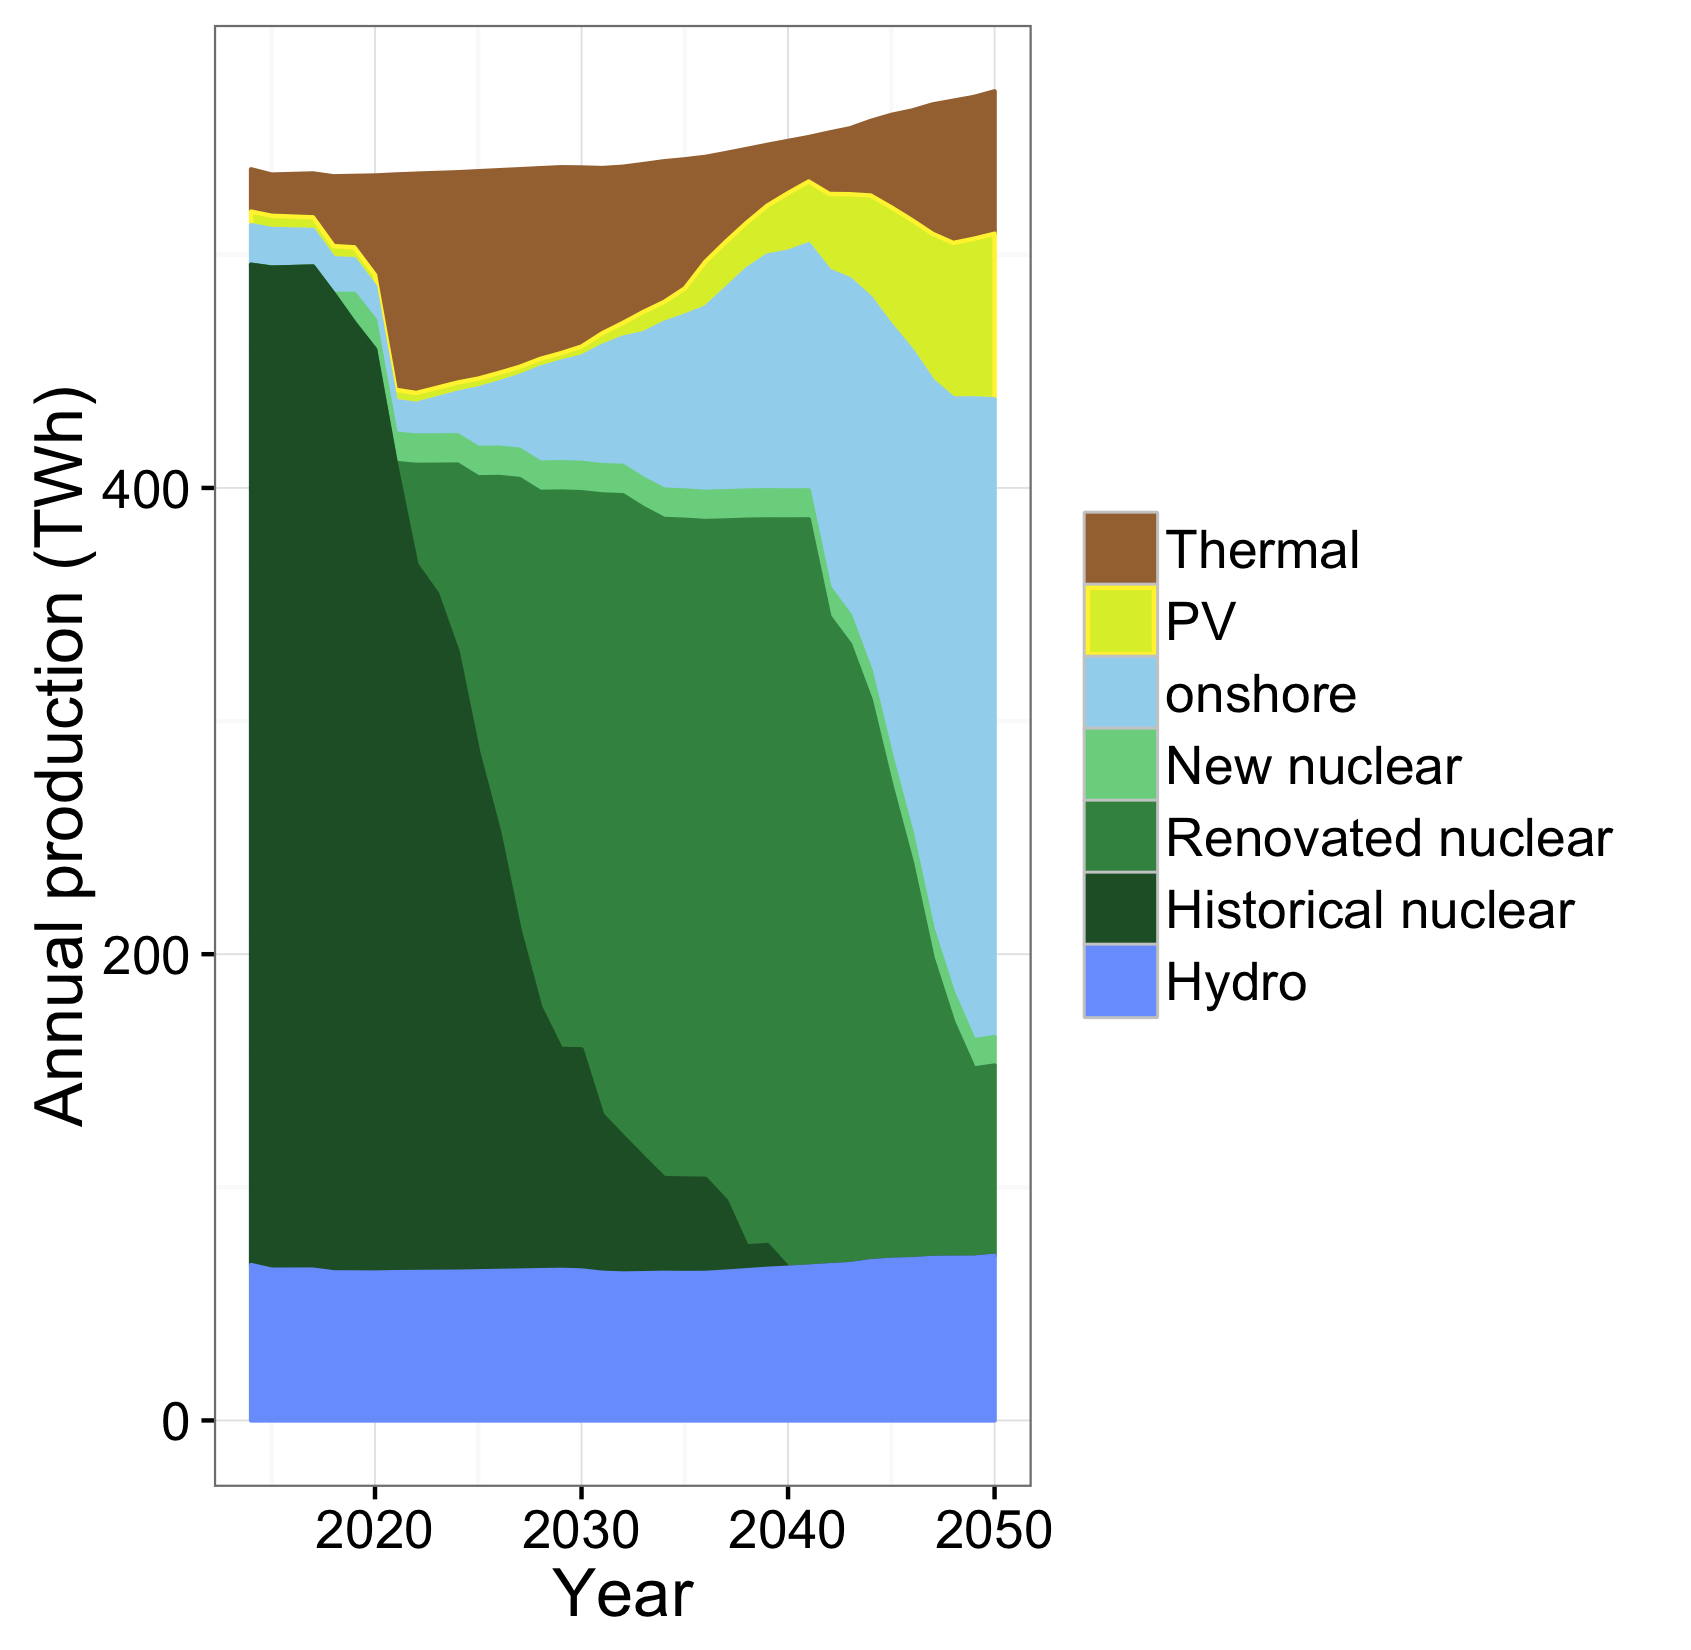
\includegraphics[height=8cm]{figures/powerMix_R80N100MedD.png}
		\label{fig:nukeShare80}
	}
	\subfloat[Optimum for retrofitted nuclear around 90 \emwh] {
		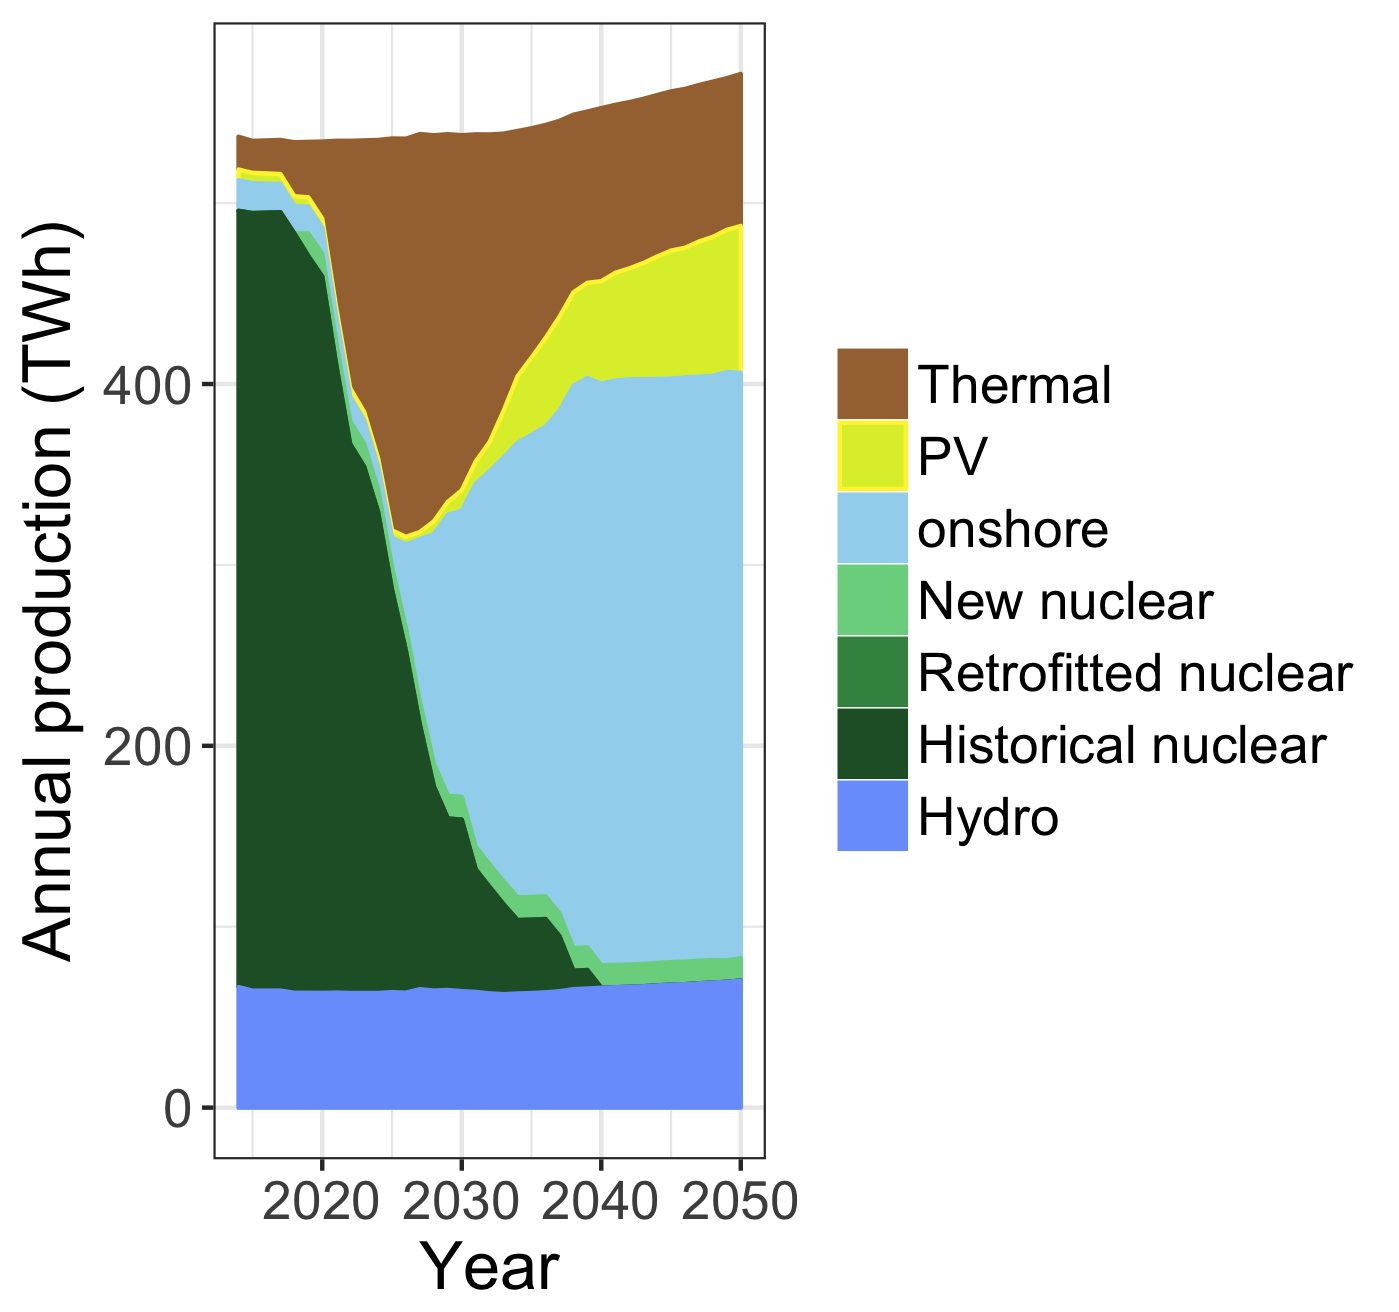
\includegraphics[height=8cm]{figures/powerMix_R90N100MedD.png}
		\label{fig:nukeShare90}
	}
	\caption{Optimum power mix for various nuclear retrofitting costs}
\end{figure}


\begin{figure}[!ht]
	\centering
	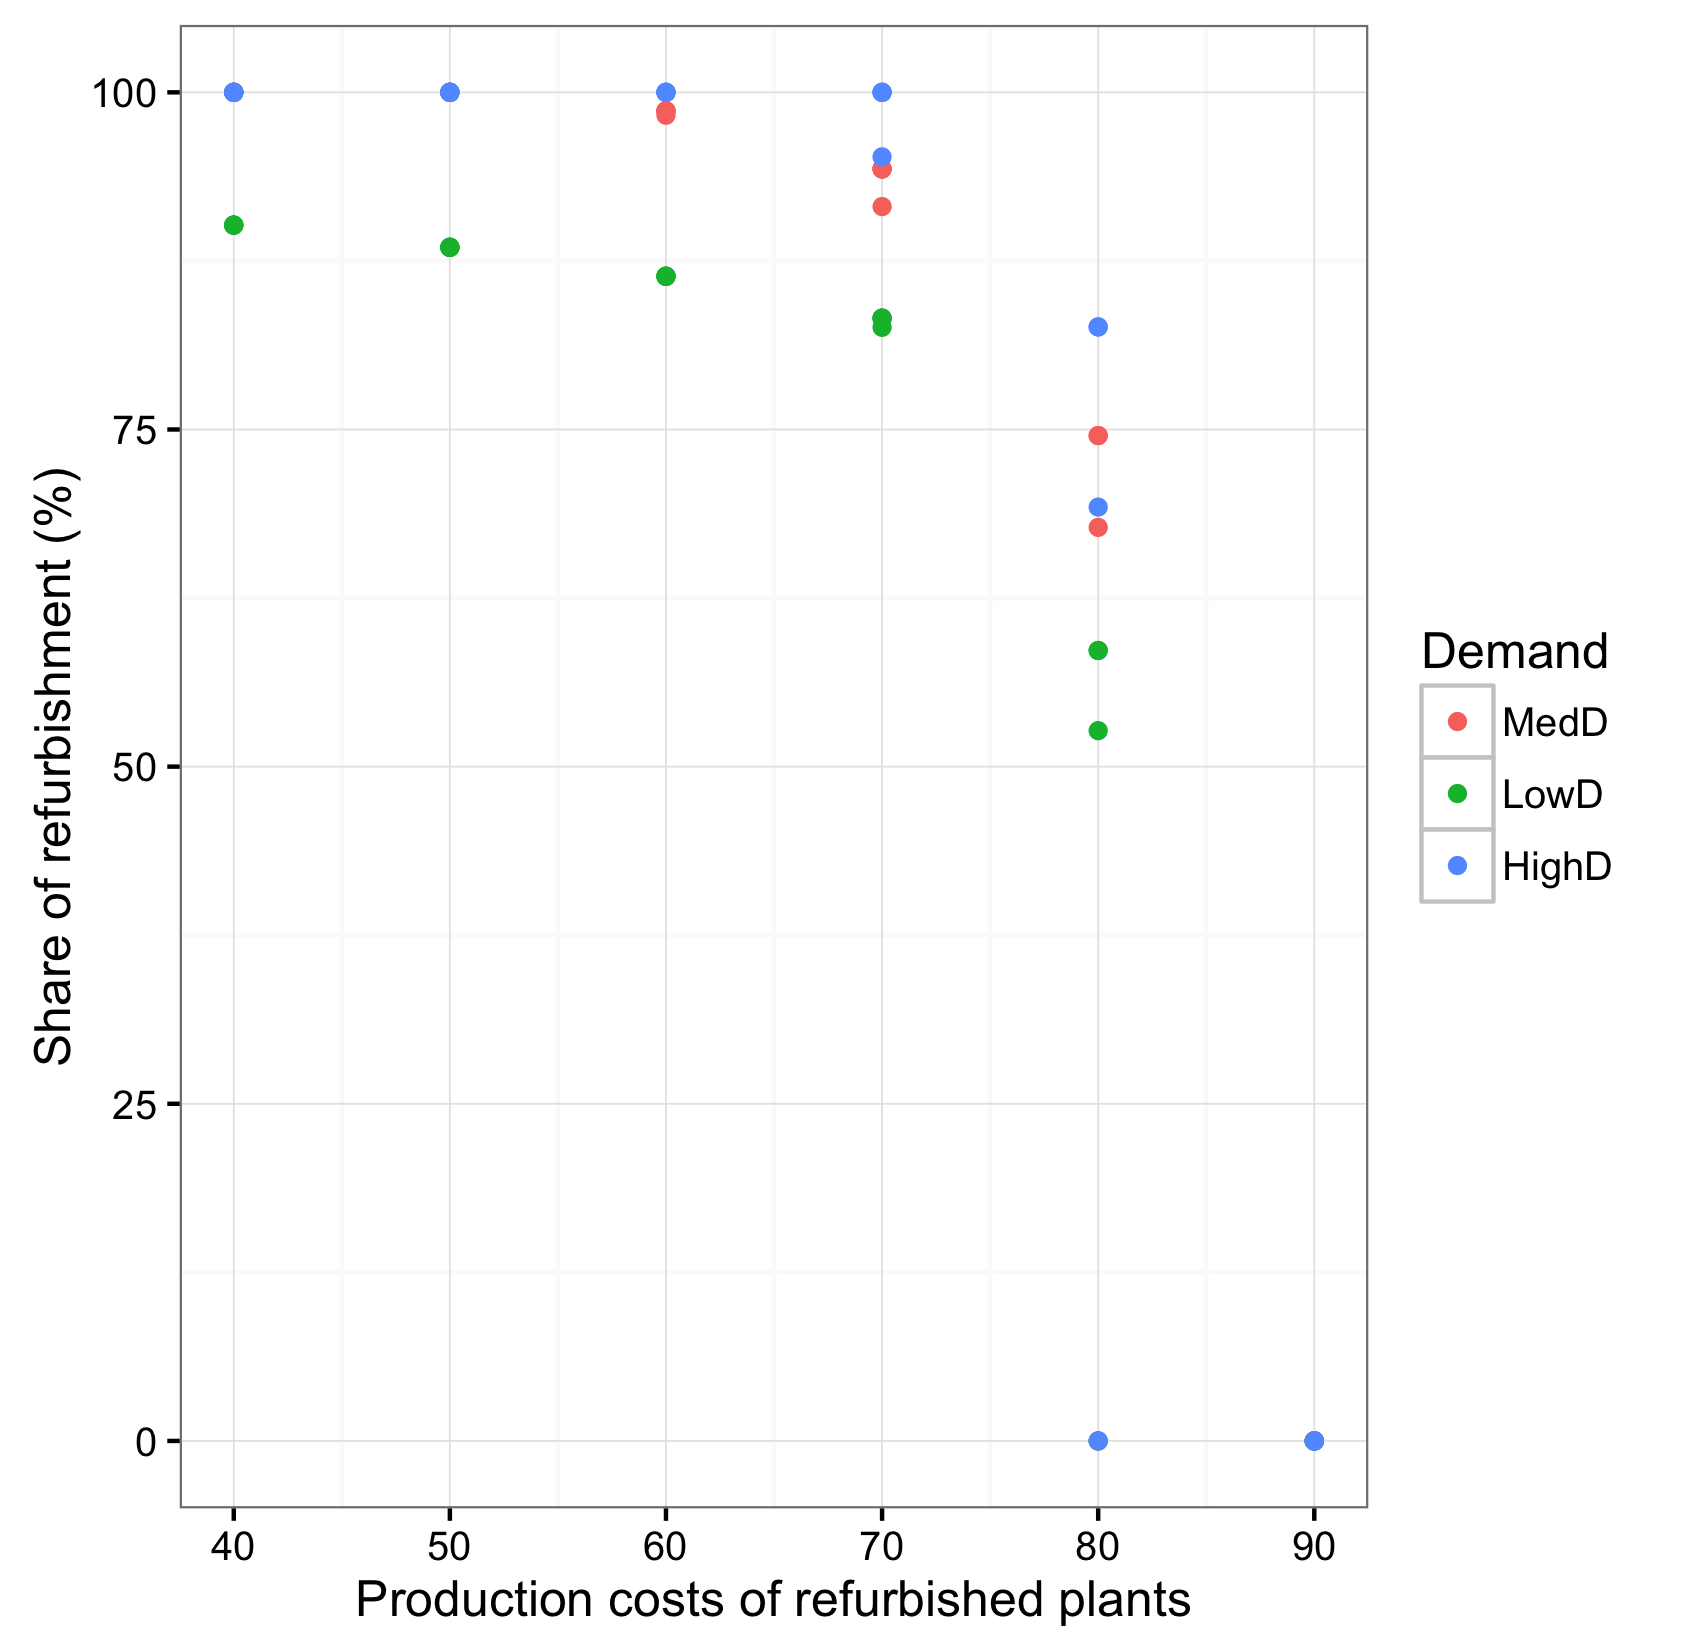
\includegraphics[height=8cm]{figures/powerMixSensitivity.png}
	\caption{Optimal nuclear shares and sensitivity analysis}
	\label{fig:powerMixSensitivity}
\end{figure}


%%%%%%%%%%%%

\clearpage

\subsubsection{Analysis with PRIM}


\subsubsection{Choice of threshold}

\begin{figure}
	\centering
	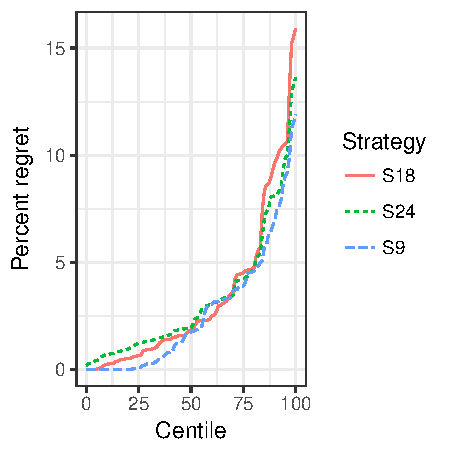
\includegraphics[width=6cm]{figures/quantile_regret.pdf}
	\caption{Ordered distribution of regret for the three candidate strategies S9, S24 and S18}
	\label{fig:quantile_regret}
\end{figure}



\subsubsection{Efficiency frontier}

\begin{figure}
	\centering
	\subfloat[With the cluster from S9] {
		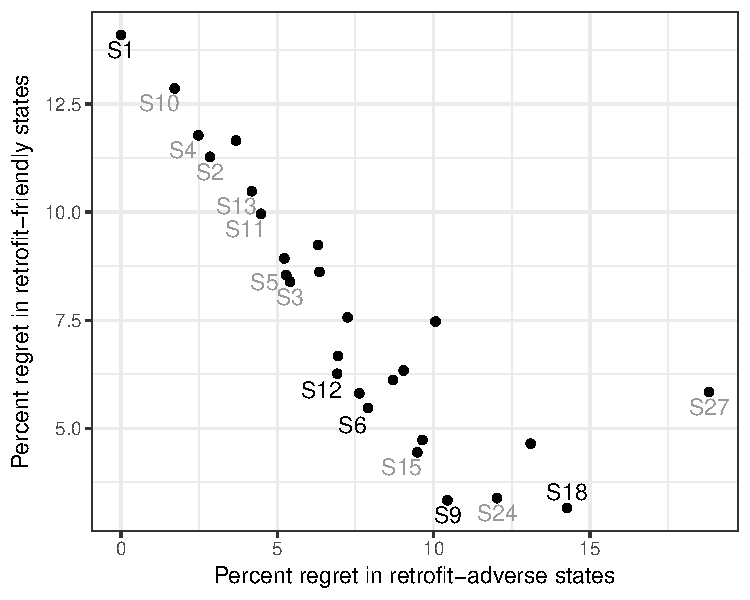
\includegraphics[width=6cm]{figures/low_regret_frontier_S9.pdf}
	}
\subfloat[With the cluster from S18 and S24] {
		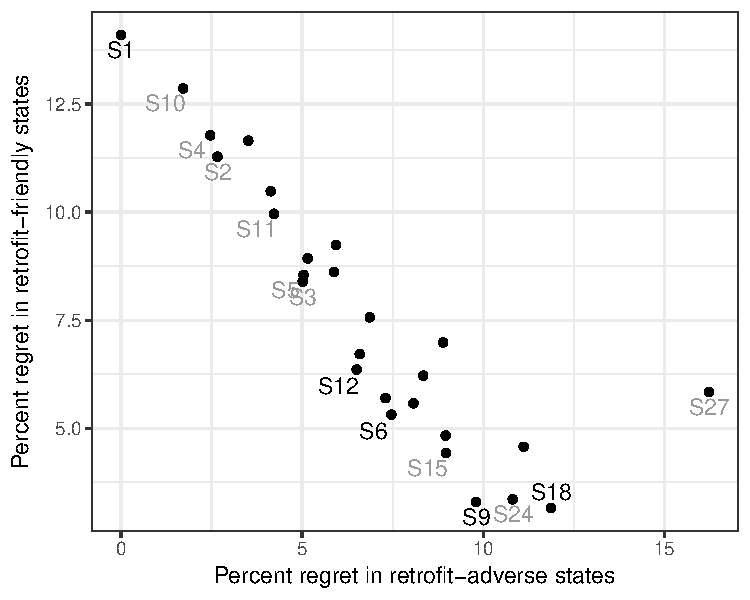
\includegraphics[width=6cm]{figures/low_regret_frontier_S18.pdf}
}
	\caption{Trade-offs and efficiency fontier using the PRIM-generated cluster from strategy S9 and strategy S18 and S24}
	\label{fig_app:low_regret_frontier}
\end{figure}


\subsubsection{Regrets of the strategies S9, S18 and S27}


\begin{figure}
	\centering
	\subfloat[Regret of the full-retrofit strategy S27] {
		\makebox[5.5cm][c]{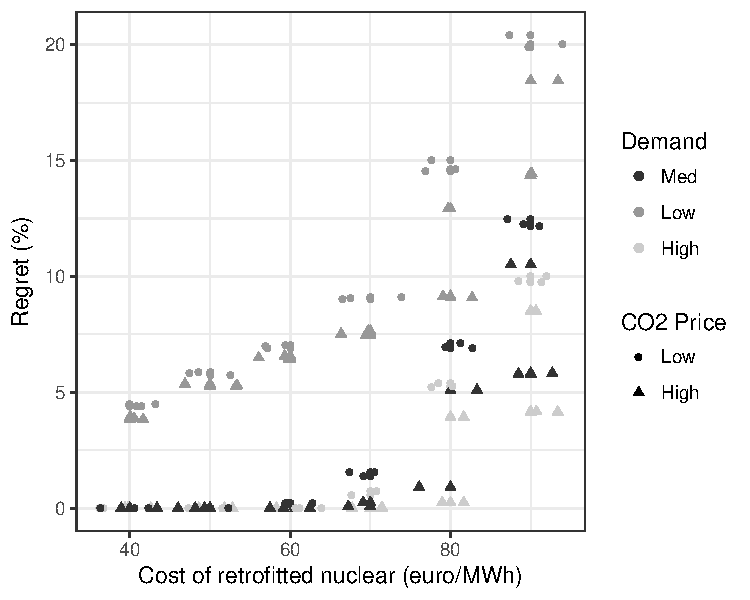
\includegraphics[height=5cm]{figures/vulnerabilities_S27.pdf}}
		\label{fig_app:vulnerabilities_S27}
	} 

	\subfloat[Regret of the full-retrofit strategy S9] {
		\makebox[5.5cm][c]{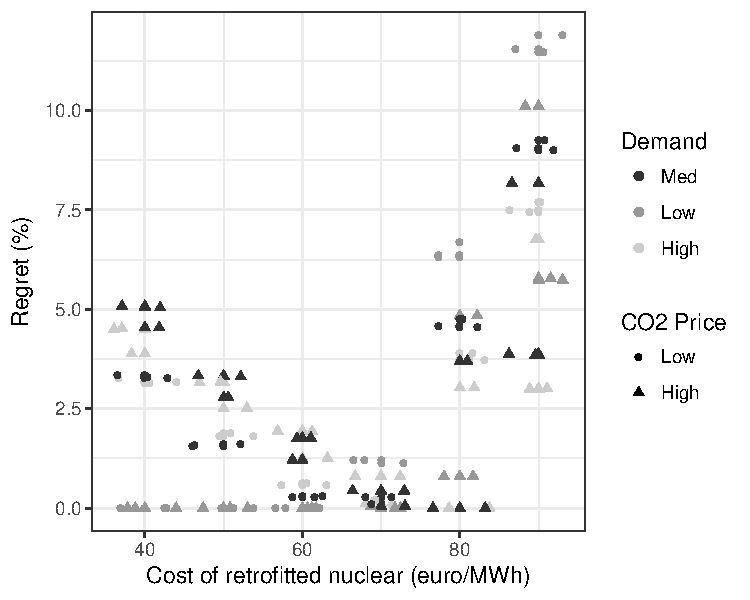
\includegraphics[height=5cm]{figures/vulnerabilities_S9.pdf}}
	} \qquad
	\subfloat[Regret of the full-retrofit strategy S18]{
		\makebox[6cm][c]{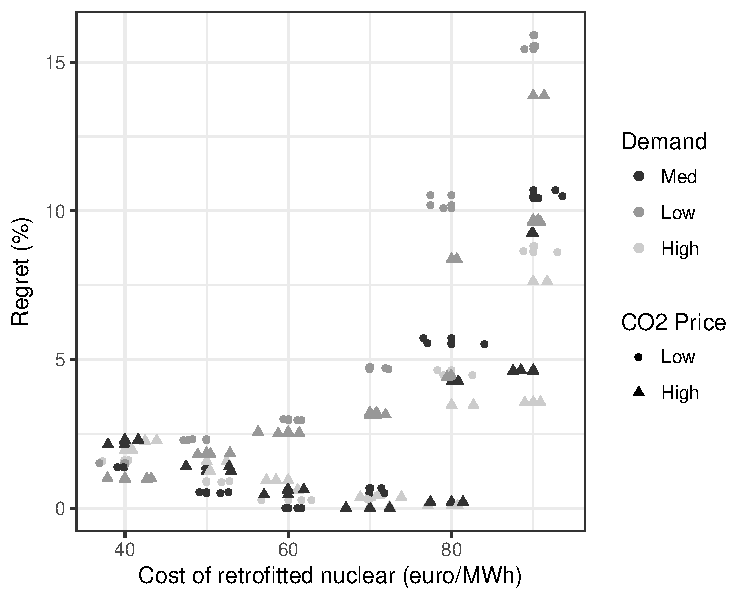
\includegraphics[height=5cm]{figures/vulnerabilities_S18.pdf}}
		\label{fig_app:vulnerabilities_S9_S18_S27}
	}
	\caption{Regret of the full-retrofit strategy S9, S18 and S27}
\end{figure}

\subsubsection{Optimal trajectory depending on implicit probabilities}

\begin{figure}
	\centering
	\subfloat[With the cluster from strategy S9] {
		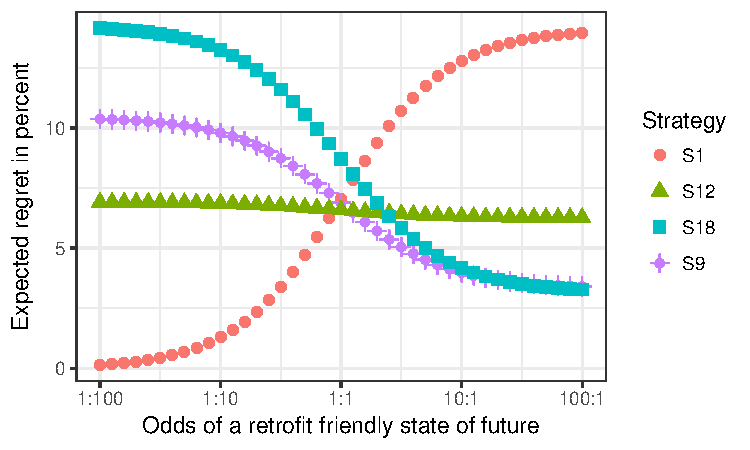
\includegraphics[width=6cm]{figures/odds_S9.pdf}	
	}
	\subfloat[With the cluster from strategy S18 and S24] {
		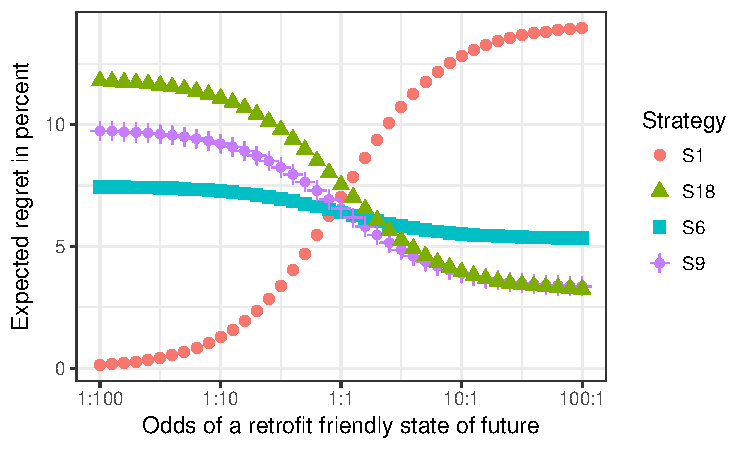
\includegraphics[width=6cm]{figures/odds_S18.pdf}	
	}
	\caption{Optimal strategy depending on the implicit odds of the decision maker}
	\label{fig_app:odds}
\end{figure}


%%%%%%%%%%%%%%%%%%%%%%%%%%%%ù
\clearpage
\subsubsection{Comparison with official scenarios}

\begin{figure}
	\centering
	\subfloat[Nuclear share (\%)] {
		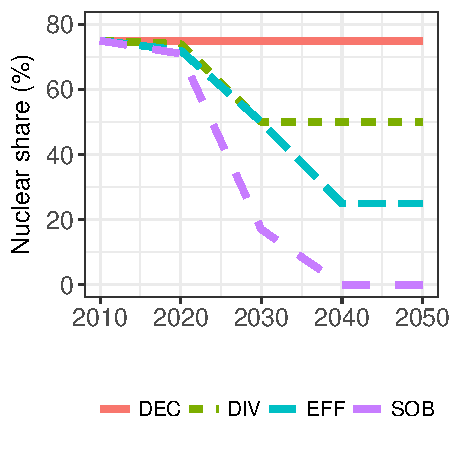
\includegraphics[height=6cm]{figures/dnte_nuc_shares.pdf}
	}
\subfloat[Demand levels (TWh/year)] {
		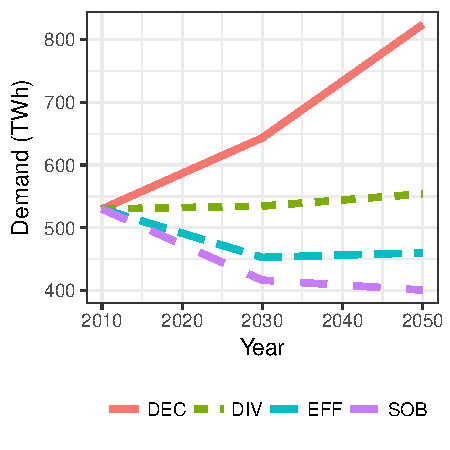
\includegraphics[height=6cm]{figures/dnte_demands.pdf}
	}
	\caption{Characteristics of the four official scenarios in the French national debate \\Source: \citet{DNTE_gt2} and authors' calculations}
	\label{fig:DNTE_scenarios}
\end{figure}


\end{subappendices}

\newrefsection
\selectlanguage{french}
\chapter{La transition énergétique est-elle favorable aux branches à fort contenu en emploi? Une analyse input-output pour la France} \label{chap:TE_Emploi}

\section{Introduction}
Dans la sphère académique, les politiques énergétiques, comme toutes les politiques sectorielles, sont principalement évaluées selon un critère coût-bénéfice ou coût-efficacité, ou encore en fonction de leur impact estimé sur le PIB, vu comme une approximation du bien-être économique. Leur impact sur l’emploi fait l’objet de moins d’analyses, comme le montre une simple consultation de la base de données académiques Web of Science : une interrogation à l’aide de la combinaison de mots-clés « energy AND (cost OR GDP OR welfare) » amène 96 549 résultats, soit 21 fois plus qu’une interrogation sur « energy AND (employment OR jobs) » (4 593 résultats). Dans le débat public français, en revanche, l’impact sur l’emploi de ces politiques a une importance équivalente à celle des analyses en termes de coût, de bien-être économique ou de PIB, comme le montre une interrogation de la base de données d’articles de presse Factiva : les mots-clés « transition énergétique AND (PIB OR coût) » renvoient 878 résultats, contre 895 pour « transition énergétique AND (emploi OR chômage) »\footnote{Interrogations effectuées le 23 septembre 2015}.

L’intérêt de prendre en compte l’emploi, plutôt que se focaliser sur le coût ou le surplus du consommateur, est double. Politiquement, de nombreux choix sont étudiés à l’aune de leur effet, réel ou supposé, sur l’emploi, donc une politique environnementale mauvaise pour l’emploi risque de ne jamais voir le jour. Par ailleurs, l’emploi présente une valeur au-delà du seul salaire \citep{Clark2015} qui renforce l’importance de cet indicateur.

Certes, les chercheurs en économie n’ont pas complètement négligé l’impact sur l’emploi de ces politiques. En particulier, une partie (minoritaire) du débat théorique sur le double dividende, initié par \citet{Pearce1991} et \citet{Goulder1994} porte sur l’emploi. \citet{Bosquet2000}, \citet{Chiroleu-Assouline2001} et \citet{Patuelli2005} proposent des revues de littérature. On peut noter l’absence de consensus dans ces travaux, avec des résultats très divers selon les hypothèses retenues. 

Avec l’essor des préoccupations liées aux changements climatiques, une attention nouvelle s’est portée sur la question des emplois liés à la transition énergétique, et en particulier aux énergies renouvelables. De nombreuses études technico-économiques comparent différentes techniques de production d’énergie (et/ou d’économie d’énergie). Plusieurs systèmes de mesure coexistent dans la littérature. Un premier est le nombre d’emploi par capacité installée, en kW. \citet{Cameron2015} passent en revue 70 études de ce type. Un autre système de mesure est le nombre d’emplois par énergie produite, en kWh. \citet{Wei2010} synthétisent ces études pour les Etats-Unis. Cependant, ces deux mesures présentent un biais en faveur des options techniques et organisationnelles les plus coûteuses : si une option coûte dix fois plus cher qu'une autre pour installer un kW ou produire un kWh, il est très probable qu'elle crée plus d'emplois par kW ou kWh, car les salaires comptent pour environ deux tiers de la valeur ajoutée \citep{Cotis2009}. Or, des agents économiques (ménages, entreprises, administrations publiques…) vont nécessairement payer pour ce surcoût et vont par conséquent réduire d'autres consommations, d’où des destructions d’emplois ignorées par ce ratio. Pour cette raison, dans la présente étude nous calculons le ratio emplois par euro de demande finale.

Par ailleurs, plusieurs études menées à l’aide de modèles macroéconomiques ont étudié l’effet sur le PIB mais aussi sur l’emploi de politiques climatiques, principalement de taxes sur les émissions de CO\textsubscript{2}. On peut citer notamment les travaux de \citet{Lehr2008}, \citet{Lehr2012} ou encore \citet{EY2015} pour le compte de l’ADEME. En France, le modèle macroéconomique Three-ME, développé par l’ADEME et l’OFCE, a été utilisé pour quantifier le scénario « visions énergétiques 2030-2050 » de l’ADEME. Il aboutit à +330 000 emplois en 2030 et +825 000 en 2050, par rapport à un scénario tendanciel \citep{ADEME2013}. Ces travaux sont utiles, mais leurs résultats sont très dépendants de diverses hypothèses qui, du fait de la complexité de ces modèles, sont peu compréhensibles hors de la communauté des modélisateurs. Ainsi, deux modèles macroéconomiques ont été utilisés pour évaluer le paquet « climat-énergie » de la Commission européenne : E3ME, de Cambridge Econometrics, et GEM-E3, de la National Technical University of Athens. Les résultats du premier modèle en termes de PIB et d’emploi sont beaucoup plus favorables, pour des raisons qu’il est difficile de saisir, au-delà d’affirmations assez générales comme l’opposition entre le caractère néokeynésien du premier et néoclassique du second \citep{Bruyn2014}.

De nombreuses autres études portant sur l'emploi utilisent des modèles input-output simples. On les retrouve dans des sujets aussi divers que les programmes d'efficacité énergétique dans le bâtiment \citep{Scott2008}, la biodiversité \citep{DeBeir2015}, le chauffage par biomasse \citep{Madlener2007}, les biocarburants \citep{Neuwahl2008} ou encore des études plus générales sur la transition énergétique \citep{Quirion2013}. 
Les mécanismes à l’œuvre dans ces travaux sont plus faciles à comprendre car c’est alors la différence de contenu en emploi (au sens du ratio emplois/euro de demande finale) entre les branches en progression et celles en régression qui détermine l’effet net sur l’emploi. Cependant, ces études n’expliquent pas l’origine des écarts de contenu en emploi entre les branches : si un contenu en emploi plus élevé dans une branche provient, par exemple, de salaires plus faibles ou de moins d’importations. 
Pourtant, la différence est importante : dans un cas, il s’agit de relocaliser des emplois ; dans l’autre, de favoriser des créations d’emplois moins rémunérés.

Dans cet article, nous ne cherchons pas à calculer l’effet sur l’emploi d’un scénario ou d’une politique de transition énergétique mais à estimer le contenu en emploi et en gaz à effet de serre des différentes branches de l’économie française, ainsi qu’à décomposer les écarts de contenu en emploi selon une série de facteurs explicatifs. Cette approche descriptive permet d’apporter un éclairage qualitatif sur quelques substitutions interbranches impliquées par la transition énergétique. Par « transition énergétique », dans tout l’article nous ne faisons pas référence à un scénario particulier, mais à une évolution vers une sortie des énergies fossiles, nécessaire pour respecter l’objectif d’une division par quatre des émissions de gaz à effet de serre en France d’ici 2050, objectif fixé dans la loi depuis 2005\footnote{Loi de programme fixant les orientations de la politique énergétique (POPE) du 13 juillet 2005}.

En termes de méthode, cet article se rapproche des études de balance en emploi, qui mobilisent également les outils d’analyse entrées-sorties afin d’évaluer l’effet des échanges internationaux sur l’emploi. Ces analyses permettent une description fine distinguant les types de branches qui contribuent aux déséquilibres, les catégories de travailleurs touchés, etc. \citep{Guimbert2002}. La même méthodologie est d’ailleurs appliquée pour étudier l’empreinte carbone de la demande finale, afin de comptabiliser les émissions directes et indirectes \citep{Xu2014, Lenglart2010}. Cette analyse est notamment appliquée à l’étude des échanges commerciaux \citep{Dong2010}.

Le même cadre comptable peut être appliqué de façon dynamique, pour voir l’évolution du nombre d’emplois en faisant apparaitre les contributions des grands facteurs explicatifs. \citet{Barlet2009} observent les contributions respectives de la productivité, de la demande intérieure, des importations et des exportations. Cette dernière méthodologie est également de plus en plus utilisée pour comprendre les évolutions des émissions de gaz à effet de serre \citep{Martin2014a}.

Notre approche s’inscrit à l’intersection de ces deux démarches. Nous utilisons le même cadre comptable, et une décomposition proche de celle de \citet{Barlet2009} mais nous nous inscrivons dans un cadre statique, à l’instar des études de balance en emploi. L’originalité de notre article est de comparer le contenu en emploi de chaque branche à la moyenne de l’économie nationale et de décomposer cet écart pour chacune des branches selon quelques facteurs explicatifs. Plutôt que d’observer l’évolution temporelle de chaque branche, nous comparons les branches à la moyenne de l’économie et, grâce à ce point de repère, les unes par rapport aux autres. 

De plus, nous calculons dans un même cadre le contenu en emploi et le contenu en émissions de gaz à effet de serre sur le territoire. Notre approche permet de visualiser quelles branches permettent de créer de l’emploi en France tout en réduisant les émissions pour respecter les engagements internationaux de la France ; mais elle n’indique pas les emplois créés hors de France, ni une empreinte carbone incluant les émissions associées aux importations et aux exportations \citep{Pasquier2012}.

La méthode entrées-sorties s'appuie sur quelques hypothèses bien connues. Une hypothèse d’homogénéité des produits d’une branche est nécessaire pour notre décomposition du contenu en emploi et pour la description statique de l’économie. Etudier les effets d’une variation de la demande finale implique d’adopter deux autres hypothèses : une hypothèse de rendements constants (la consommation additionnelle ne modifie pas le système productif et le progrès technique n'est pas inclus) et une hypothèse que les effets induits autre que ceux capturés par la matrice de Leontief sont négligeables \citep{Freyssinet1977}. Ces hypothèses doivent amener à être prudent sur l’interprétation des résultats, et impliquent de ne considérer ni des variations trop importantes de la demande, ni un horizon temporel trop lointain.
Sous réserve de ces hypothèses supplémentaires, notre approche descriptive pourra être utilisée de façon plus normative, dans le but de guider l’action publique en donnant une idée des effets de premier ordre liés à une réallocation de la demande finale.

Le plan retenu est le suivant : nous présentons la méthode et les données utilisées dans la partie  \ref{sec:methode_donnees}, les résultats dans la partie \ref{sec:resultats}, puis nous concluons.


\section{Méthode et données}
\label{sec:methode_donnees}

\subsection{Données}
Nous utilisons trois sources de données, toutes publiées par Eurostat et concernant la France en 2010. Elles utilisent la nomenclature NACE rév. 2 en 64 branches.
\begin{itemize}
	\item Premièrement, le tableau entrées-sorties (TES) pour la France, au niveau de désagrégation A64, pour l’année 2010, à prix courant, préparé par l’Insee et publié par Eurostat (code Eurostat \href{http://appsso.eurostat.ec.europa.eu/nui/show.do?dataset=naio_cp18_r2&lang=en}{naio\_cp18\_r2}). Nous utilisons les tableaux fournis par Eurostat et non par l’INSEE pour trois raisons : la désagrégation est supérieure, avec 64 niveaux contre 38 pour les TES actuellement publiés par l’Insee (le TES à 118 branches n’est plus publié par l’Insee depuis 2007) ; l’utilisation des données Eurostat permet d’appliquer à notre analyse à tout pays européen ou à l’UE ; et ce TES distingue les consommations intermédiaires importées de celles produites en France, ce qui est indispensable pour calculer le contenu en emploi. Nous utilisons le tableau à prix courants car nous ne cherchons pas à étudier une évolution, mais la structure de l’économie pour une année donnée.
	\item Deuxièmement, l’emploi en équivalent temps plein (ETP), code Eurostat \href{http://appsso.eurostat.ec.europa.eu/nui/show.do?dataset=nama_nace64_e&lang=en}{nama\_nace64\_e}. Ces données fournissent le détail entre emploi salarié et emploi non-salarié. 
	\item Troisièmement, les comptes physiques d’émissions ventilés par branche économique pour la France, préparés par le Citepa et le SOeS et diffusés par Eurostat. Les gaz à effet de serre inclus sont ceux couverts par le Protocole de Kyoto : CO\textsubscript{2}, CH\textsubscript{4}, N\textsubscript{2}O, PFC, HFC et SF\textsubscript{6} (code Eurostat \href{http://appsso.eurostat.ec.europa.eu/nui/show.do?dataset=env_ac_ainah_r2&lang=en}{env\_ac\_ainah\_r2}). Nous les agrégeons en tonnes équivalent-CO\textsubscript{2} en utilisant les potentiels de réchauffement global utilisés par le protocole de Kyoto (21 pour le CH\textsubscript{4}, 310 pour le N\textsubscript{2}O). 
\end{itemize} 
Enfin, nous corrigeons le TES afin d’inclure les revenus non-salariés du travail dans les compensations. L'emploi non-salarié recouvre les employeurs, les personnes établies à leur compte, les membres des coopératives de production et les travailleurs familiaux non rémunérés. Nous utilisons les données d'Eurostat sur le nombre d'ETP non-salariés, et nous le traduisons en revenus salariés équivalents en supposant un même revenu par ETP pour salariés et non-salariés. Nous le faisons afin de tenir compte des nombreux travailleurs non-salariés, notamment dans la branche agriculture.

\subsection{Définition du contenu en emploi}
Suivant en cela une longue tradition \citep{Freyssinet1977, Husson1994}, nous définissons le contenu en emploi comme le nombre d’emplois (plus précisément d’ETP) localisés en France, nécessaires à la production générée par un million d’euros de demande finale adressé à une branche donnée et pour une année donnée. Ce nombre d’emplois comprend des emplois directs (c’est-à-dire dans la branche à laquelle s’adresse cette demande finale) et indirects (dans les branches en amont de cette dernière). Ainsi défini, le contenu en emploi correspond au terme de multiplicateur d’emploi qui existe également dans la littérature \citep{Miller2009}.

Nous choisissons donc de définir le contenu en ETP d’une branche i par :
\begin{equation}
ce_i= \frac{\text{Nombre d'ETP directs et indirects dus à l'activité de la branche i}}{\text{Millions d'euros de demande finale adressée à la branche i}}
\label{definition_ce}
\end{equation}
Cette méthode est préférable aux ratios emplois/chiffre d’affaire ou emplois/valeur ajoutée : le premier présente un biais au détriment des branches utilisant une forte proportion de consommations intermédiaires, donc d’emplois indirects, tandis que le second est imprécis car il ne distingue pas deux branches ayant le même ratio emplois/VA mais adressant leurs demandes de consommations intermédiaires à des branches présentant elles-mêmes un contenu en emploi différent, donc générant au total un nombre différent d’emplois.

\subsection{Calcul du contenu en emploi}
L’utilisation des tableaux entrées-sorties (TES) de la comptabilité nationale permet de calculer le contenu en emploi pour les différentes branches de l’économie, en nous appuyant sur la méthode de \citet{Leontief1986}. Le point de départ de cette méthodologie est l’équilibre comptable entre ressources et emplois pour les produits de chaque branche, pour une année donnée. Les données permettent en outre de distinguer un équilibre correspondant au territoire nationale (ou part intérieure), représenté dans l'équation \ref{equilibre_interieur}, et un équilibre pour les importations, dans l'équation \ref{equilibre_imports} :
\begin{equation}
\pmb{p^d} = \pmb{CI^d} \cdot \pmb{i} + \pmb{d^d}	
\label{equilibre_interieur}
\end{equation}
\begin{equation}
\pmb{m} = \pmb{CI^m} \cdot \pmb{i} + \pmb{d^m}	
\label{equilibre_imports}
\end{equation}
où l'exposant \textit{d} fait référence à une part intérieure (ou domestique) et l'exposant \textit{m} à une part importée. $\pmb{p^d}$ indique la production intérieure, $\pmb{CI^d}$ et $\pmb{CI^m}$ sont les matrices des consommations intermédiaires intérieures et importées, $\pmb{d^d}$ et $\pmb{d^m}$ les demandes finales intérieures et importées et $\pmb{m}$ les importations de biens finaux. $\pmb{i}$ est le vecteur colonne composé uniquement de 1. Les notations suivent les conventions suivantes : les lettres en gras et minuscules d’imprimerie indiquent un vecteur-colonne, les capitales d’imprimerie en gras une matrice carrée. Enfin, on réserve l'exposant \textit{t} pour les valeurs totales, somme des valeurs intérieures et importées. Ainsi, la demande finale totale $\pmb{d^t=d^d+d^m}$ et l'ensemble des consommations intermédiaires vaut $\pmb{CI^t=CI^d+CI^m}$.


On peut introduire les matrices des coefficients techniques $A^d$ et $A^m$, c'est-à-dire les matrices telles que :
\begin{equation*}
A^d = (A^d_{ij}) = \left( \frac{CI^d_{ij}}{P_j} \right) \quad \text{et} \quad A^m = (A^m_{ij}) = \left( \frac{CI^m_{ij}}{P_j} \right)
\end{equation*}
En utilisant ces matrices de coefficients techniques, on peut réarranger les équations \ref{equilibre_interieur} et \ref{equilibre_imports} afin d'obtenir une relation liant directement la production à la demande finale :
\begin{equation}
\pmb{p^d} = (\pmb{I} - \pmb{A^d})^{-1} \cdot \pmb{d^d}	
\label{equilibre_interieur2}
\end{equation}
où $\pmb{I}$ est la matrice identité. La matrice $(\pmb{I} - \pmb{A^d})^{-1}$ est la matrice inverse de Leontief. 
Elle indique la production directe et indirecte nécessaire pour satisfaire une demande intérieure. 
Plus précisément, le terme d'indices (i,j) de cette matrice $(\pmb{I} - \pmb{A^d})^{-1}$ donne la production dans la branche $i$ engendrée par unité de demande finale adressée à la branche $j$.

L'équation \ref{equilibre_interieur2} donne la somme de la production dans chaque branche générée par le vecteur de demande finale. On peut cependant affiner cette formule afin d'extraire plus d'information. Pour cela, on introduit l'opérateur $\widehat{  }$ qui transforme un vecteur colonne en matrice carrée diagonale. L'équation \ref{equilibre_interieur2} devient :
\begin{equation}
\pmb{P^d} = (\pmb{I} - \pmb{A^d})^{-1} \cdot \widehat{\pmb{d^d}}	
\label{equilibre_interieur3}
\end{equation}
Dans cette nouvelle version, on obtient une matrice carrée $\pmb{P^d}$ pour la production intérieure. Le terme d'indice (i,j) de cette matrice indique la production générée dans la branche $i$ du fait de la demande adressée à la branche $j$.

Enfin, on peut lier la production à la demande totale, et non à la seule demande intérieure. Cet ajout permet de voir l'impact des importations finales. On suppose que le taux $MF_i = \frac{D^d_i}{D^t_i}$ de demande intérieure dans la demande finale totale $\pmb{d^t}$ est constant pour chaque branche $i$ - autrement dit, on suppose que le taux d'importations finales dans la demande finale totale, $1 - MF_i$, est constant pour chaque branche. De façon matricielle, on peut l'écrire $\pmb{d^d} =~\widehat{\pmb{mf}} \cdot~\pmb{d^t}$, avec $\pmb{mf}$ le vecteur colonne des taux d'importations. Alors, l'équation \ref{equilibre_interieur3} devient :
\begin{equation}
\pmb{P^d} = (\pmb{I} - \pmb{A^d})^{-1} \cdot \widehat{\pmb{mf}} \cdot \widehat{\pmb{d^t}}	
\label{equilibre_interieur4}
\end{equation}

Maintenant, si l'on connait le nombre d'ETP $ETP_j$ dans chaque branche $j$, et que l'on admet que ce nombre d'emplois est proportionnel à la quantité $P_j$ produite, alors on peut définir la matrice colonne du nombre d'emplois par unité de production : 
$$\pmb{e} = (e_j) = ( \frac{ETP_j}{P_j})$$

Le lien entre le nombre d'emplois et la demande finale se déduit alors de \ref{equilibre_interieur4} :
\begin{equation}
\pmb{etp} =~\widehat{\pmb{d^t}} \cdot~\widehat{\pmb{mf}} \cdot~(\pmb{I} - (\pmb{A^d})^T)^{-1} \cdot \pmb{e}
\label{emploi}
\end{equation}
où $^T$ désigne l'opérateur de transposition matricielle.
Le contenu en emploi, défini dans l'équation \ref{definition_ce} comme le nombre d'emplois par unité de demande finale, découle de l'équation \ref{emploi} en posant une demande finale unitaire, autrement dit $\widehat{\pmb{d^t}}~= \pmb{I}$. On aboutit à la formule du contenu en emploi $\pmb{ce}$: 
\begin{equation}
\pmb{ce} = ~\widehat{\pmb{mf}} \cdot~(\pmb{I} - (\pmb{A^d})^T)^{-1} \cdot \pmb{e}
\label{contenu_emploi}
\end{equation}
où le terme $ce_i$ est le contenu en emploi de la branche $i$. C'est cette formule qui est utilisée pour calculer le contenu en emploi d'une branche.



\subsection{Décomposition du contenu en emploi}

Les calculs de contenu en ETP font apparaitre de fortes disparités entre les branches (cf. annexe \ref{app:tableau_ce}). Il est cependant utile de ne pas s’arrêter à la valeur du contenu en emploi, mais de détailler sa composition. Le contenu en emploi d’une branche peut en effet avoir une signification très différente s’il est faible du fait de salaires élevés ou d’importations importantes : dans le premier cas, déplacer la demande adressée à cette branche revient à réduire les salaires ; dans le second, à relocaliser la production. Une analyse détaillée du contenu en emploi est donc nécessaire dès lors que l’on souhaite utiliser cet indicateur.

Les données de la comptabilité nationale fournissent de nombreuses informations pour décomposer le contenu en emploi des différentes branches. La formule \ref{contenu_emploi} permet de déterminer directement le contenu en emploi, mais il est possible de faire apparaitre des ratios intermédiaires utiles à l'analyse.

Tout d'abord, on peut décomposer le terme $\pmb{e}$ donnant le nombre d'emplois par unité de production. Plutôt que de passer directement de l'emploi à la production, on va chercher à faire apparaitre l'importance des taxes dans la valeur ajoutée, la part des salaires par rapport aux revenus du capital, et le niveau de salaires.
Le second terme à décomposer est $(\pmb{I} - (\pmb{A^d})^T)^{-1}$, afin de faire apparaitre les importations intermédiaires. En effet, comme $\pmb{A^d} = \pmb{A^t} - \pmb{A^m}$, la production intérieure va dépendre à la fois des fonctions de production représentées dans $\pmb{A^t}$ et des taux d'importations reflétés par $\pmb{A^m}$.

\begin{equation}
\forall i \quad ce_i = \sum_j MF_i \cdot V_{ij} \cdot MI_{ij} \cdot T_j \cdot L_j \cdot N_j
\end{equation}
où
\begin{itemize}
	\item $MF_i $ est le taux de demande intérieure dans la demande finale totale ;
	\item $V_{ij}$ est la valeur ajoutée intérieure par unité de production ;
	\item $MI_{ij}$ indique le taux d'importations intermédiaires ;
	\item $T_j$ est le taux de taxes et subventions (« Autres impôts sur la production », code D29\_M\_D39 et « Impôts moins subventions sur les produits », code D21\_M\_D31) dans la valeur ajoutée augmentée des « Impôts moins subventions sur les produits »;
	\item $L_j$ représente la part des rémunérations du travail dans la valeur ajoutée moins les « autres impôts sur la production » (D29\_M\_D39) ;
	\item $N_j$ est égal à l’inverse du salaire. Il mesure donc le niveau des salaires.
\end{itemize}

Cette suite de ratio en cascade suit une logique de production illustrée par la figure \ref{fig:schema_decompo}.

\begin{figure}[!hb]
	\centering
	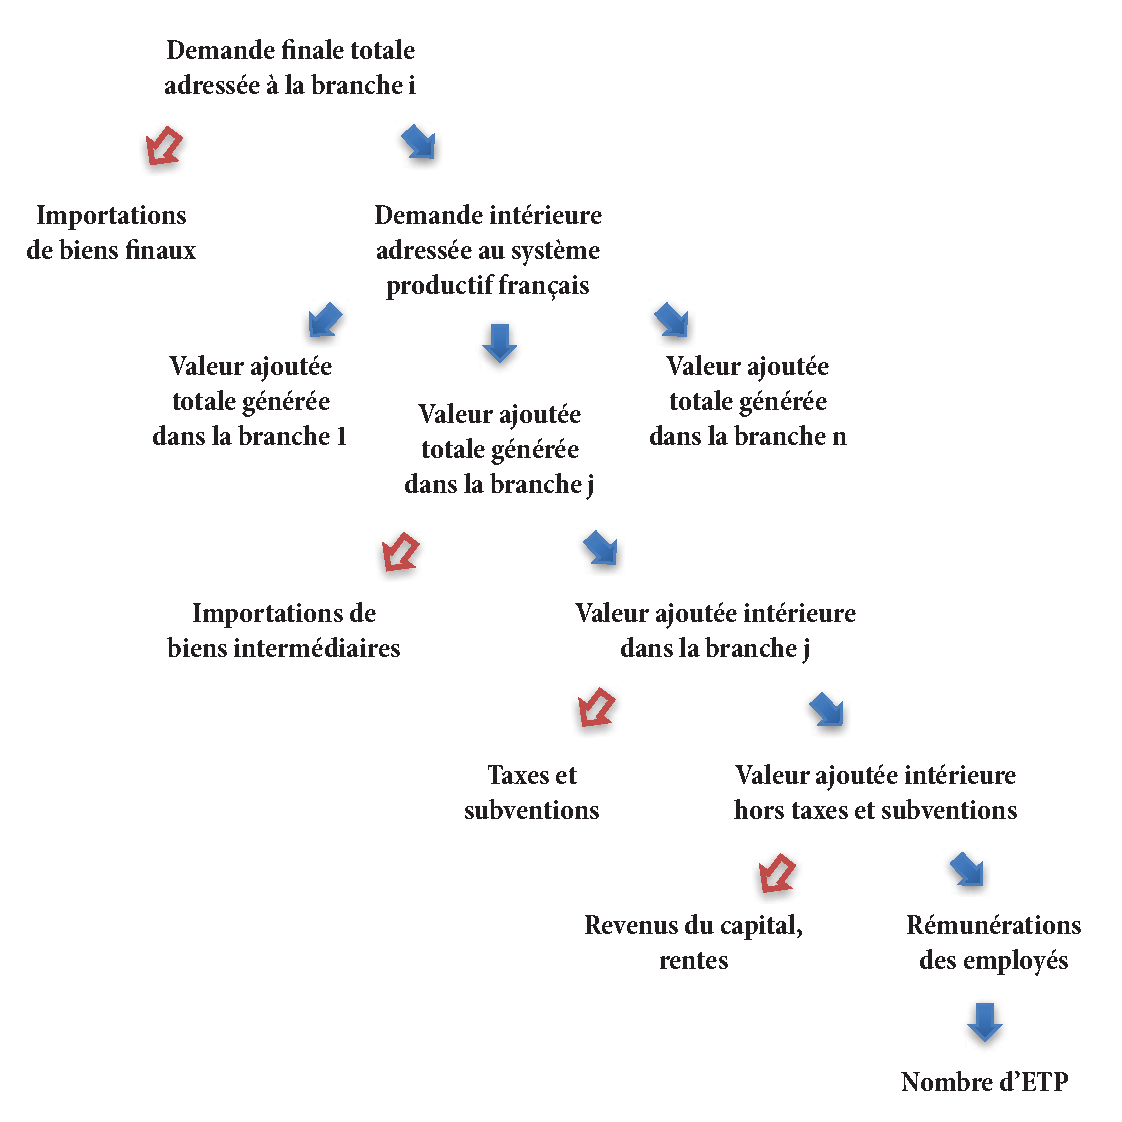
\includegraphics[height=12cm]{figures/Schema_decompo/schema_decompo.pdf}
	\caption{Schéma de décomposition du contenu en emploi. \\Source : Auteurs}
	\label{fig:schema_decompo}
	\captionsetup{justification=raggedright}
	\caption*{Lecture : une demande finale totale va susciter d’une part des importations finales, et d’autre part une demande intérieure qui sera adressée à la production intérieure. La demande intérieure suscite une production dans d’autres branches du fait des consommations intermédiaires, et donc la création de valeur ajoutée dans plusieurs branches. Une partie de cette valeur ajoutée est captée à l’étranger à cause des importations de produits intermédiaires. Dans la valeur ajoutée intérieure restante, une partie sert à payer des taxes ou provient de subventions. Enfin, la valeur ajoutée hors taxes et subventions rémunère le capital et les compensations salariales. Ces dernières servent à employer des travailleurs.}
\end{figure}

\subsection{Comparaison à la moyenne et décomposition LMDI}
Pour toute branche $i$, on peut comparer le contenu en emploi de cette branche avec la moyenne de l’économie nationale – cette moyenne nationale étant définie via des ratios moyens (la définition précise est donnée en annexe \ref{app:def_moyenne}).
\begin{equation}
ce_i - ce_{i,m} = \sum_j MF_i \cdot V_{ij} \cdot MI_{ij} \cdot T_j \cdot L_j \cdot N_j - \sum_j MF_m \cdot V_{ij,m} \cdot M_{ij,m} \cdot T_m \cdot L_m \cdot N_m
\end{equation}
En remarquant que les coefficients $V_{ij}$ jouent le rôle de clé de ventilation, et en utilisant la méthode LMDI (Logarithm Mean Divisia Index) de décomposition d’indice développée par \citet{Ang2005}, on peut transformer cette différence en somme de termes traduisant l’apport de chaque facteur (les détails sont donnés en annexes \ref{app:ventilation_LMDI} et \ref{app:decompo_LMDI}) :
\begin{equation}
ce_i - ce_{i,m} = \Delta MF_i + \Delta MI_i + \Delta T_i +\Delta L_i + \Delta N_i
\end{equation}
Il est ainsi possible de déterminer l’impact des différents facteurs dans la composition et le niveau du contenu en ETP. On peut donc répondre à la question : pourquoi le contenu en emploi d’une branche est-il élevé ? Est-ce du fait d’importations finales ou intermédiaires faibles, de taxes faibles, d’une forte part du travail dans la valeur ajoutée, ou de salaires bas ?


\subsection{Contenu en gaz à effet de serre}
Le contenu en émissions de gaz à effet de serre est calculé avec la même méthode que pour le contenu en emploi. A partir des émissions de gaz à effet de serre par branche, on construit le vecteur $\pmb{g}$ donnant le ratio des émissions de gaz à effet de serre (GES) par unité de production. Alors, le contenu en émissions directes et indirectes $\pmb{cg}$ est donné par la relation :
\begin{equation}
\pmb{cg} =~\widehat{\pmb{mf}} \cdot~(\pmb{I} - (\pmb{A^d})^T)^{-1} \cdot \pmb{g}
\end{equation}
Il convient de noter que notre approche traite les émissions du point de vue de la production, c’est-à-dire aux émissions sur le territoire. Notamment, nous n’intégrons pas les émissions associées aux importations. Ce choix permet d’analyser les leviers utiles aux politiques publiques pour tenir leurs engagements nationaux ou européens. En revanche, une logique cherchant à attribuer les émissions aux consommateurs – par exemple avec la notion d’empreinte carbone - devrait également prendre en compte les émissions associées aux importations \citep{Pasquier2012}. En outre, en regardant les émissions par branche d’activité, nous omettons les émissions liées aux consommations finales, notamment dans les transports intérieurs et le chauffage. 


\subsection{Branches pour lesquelles la méthode est inapplicable}
Nous appliquons la méthodologie en utilisant le tableau entrées-sorties d’Eurostat à 64 branches. Toutefois, notre méthodologie ne peut pas être appliquée à quatre branches de la nomenclature NACE Rév. 2 :
\begin{itemize}
	\item La branches B (« Industries extractives ») car la demande finale intérieure est négative en 2010, à cause des variations de stock. On ne peut donc pas prendre le logarithme de cette demande ;
	\item La branche K66 (« Activités auxiliaires de services financiers et d'assurance ») qui n’a aucune demande finale ni intérieure. Là encore, on ne peut pas prendre le logarithme ;
	\item La branche L68A (« Loyers imputés des logements occupés par leur propriétaire ») qui ne verse aucun salaire ;
	\item La branche T (« Activités des ménages en tant qu'employeurs ; activités indifférenciées des ménages en tant que producteurs de biens et services pour usage propre ») qui n’utilise aucune consommation intermédiaire. 
\end{itemize}

Par la suite, nous ignorons donc ces quatre branches, ce qui n’est pas gênant car trois de ces branches (43, 45, 64) constituent des branches particulières de l’économie, et la branche 4 présente une activité très réduite en France (inférieure à 0,13\% des ressources totales de l’économie).


\section{Résultats}
\label{sec:resultats}

\subsection{Principaux déterminants des différences de contenu en emploi}
Quels sont les grands déterminants permettant d’expliquer les différences de contenu en emploi entre les différentes branches économiques ? Pour répondre à cette question, il suffit de calculer, sur l’ensemble des branches considérées, l’écart-type de nos cinq facteurs explicatifs : plus celui-ci est élevé, plus ce facteur diffère d’une branche à l’autre et plus il explique une part importante des écarts de contenu en emploi entre les branches.

\begin{table}[!h]
	\centering
	\caption{Ecart-type des cinq facteurs explicatifs des écarts de contenu en emploi, 
		sur les 60 branches considérées. \\ 
		Source : calculs des auteurs à partir de données Eurostat.}
	\label{tab:ecart_type}
	\begin{tabular}{ll}
		\toprule
		Facteur explicatif & Ecart-type \\
		\midrule
		$\Delta N$ & 3,12 \\
		$\Delta L$ & 2,34 \\
		$\Delta MF$ & 1,67 \\
		$\Delta MI$ & 0,98 \\
		$\Delta T$ & 0,80 \\
		\bottomrule
	\end{tabular}
\end{table}


Comme l’indiquent les chiffres du tableau \ref{tab:ecart_type}, la principale cause de variation de contenu en ETP réside dans la différence de salaires, suivie de la part du travail dans la valeur ajoutée, puis, dans l’ordre, du taux d’importations de produits finaux et intermédiaires. Enfin, les taxes nettes des subventions jouent un rôle mineur dans l’explication des variations de contenu en emploi entre les différentes branches. Ce paramètre est notamment important dans la branche agriculture, du fait des subventions de la politique agricole commune.


\subsection{Contenu en emploi et en émissions de gaz à effet de serre}

Ayant obtenu le contenu en émissions de GES, nous pouvons le croiser sur un graphique avec le contenu en emploi sur la figure \ref{fig:ges_emploi}. En faisant apparaitre la moyenne de l’économie (les lignes horizontale et verticale), on peut distinguer quatre quadrants, selon nos deux critères que sont le contenu en emploi et le contenu en GES :
\begin{itemize}
	\item Le cadran en haut à droite regroupe les branches à fort contenu en emploi et en GES. La plupart de ces branches sont liées à l’alimentation. On voit ainsi que l’agriculture présente de loin le contenu en GES le plus élevé parmi les branches de l’économie française, du fait des émissions de protoxyde d’azote (N\textsubscript{2}O) et de méthane (CH\textsubscript{4}). De plus, l’industrie agroalimentaire et l’agriculture se classent en tête quant aux émissions de GES totales générées de façon directe et indirecte, émissions indiquées par la taille des cercles. La pêche, l’hébergement-restauration et les transports terrestres (fret et services de transport) figurent également dans ce cadran. 
	\item En haut à gauche se trouvent les branches fortement émettrices et générant peu d’emplois. Cela inclut l’industrie chimique, la production d’électricité, les transports aériens, la métallurgie, les activités de cokéfaction et raffinage, le traitement des eaux usées, la production de produits minéraux non métalliques (ciment, verre…), les transports par eau et l’industrie du papier.
	\item Le cadrant en bas à droite regroupe les branches ayant un contenu en emploi élevé et un contenu en émissions de GES faible. Ce groupe inclut la plupart des activités du secteur tertiaire, mais également quelques branches du secteur secondaire, notamment la construction.
	\item En bas à gauche se trouvent les branches peu créatrices d’emplois, mais également peu émettrices. Ce groupe inclut de nombreuses industries, notamment de fabrication (textile, bois, caoutchouc), de produits métalliques, informatiques ou d’équipements électriques ; mais également de nombreuses branches des services.
\end{itemize}

Sur la figure \ref{fig:ges_emploi}, nous avons indiqué en gris foncé les branches couvertes par le système communautaire d’échange de quotas d’émissions de GES (EU ETS ou SCEQE). Aujourd’hui, ce système concerne plus de 11 000 installations, et couvre presque 45\% des émissions de gaz à effet de serre de l’Union Européenne. Les branches économiques concernées sont notamment la production d’électricité, la fabrication de produits métalliques, le raffinage de produits pétroliers, la production de ciment, verre, chaux et céramique, d’acides et de produits chimiques, ainsi que le transport aérien pour les seuls vols intracommunautaires \citep{EuropeanUnion2013}.

S’il est logique que les branches couvertes par l'EU ETS se trouvent dans la partie haute de cette figure, du fait de leur fort contenu en GES, il est frappant de constater que toutes se trouvent également à gauche de celle-ci, témoignant de leur faible contenu en emploi. Ce faible contenu en emploi s'explique principalement du fait d'importations élevées et/ou d'une faible part des salaires dans la valeur ajoutée (cf. annexe \ref{app:EU_ETS}).
Plus généralement, le faible contenu en emploi de ces branches rejoint le débat sur la complémentarité de l’énergie au capital et au travail. Cette question a fait l’objet de controverses depuis les années 1970 (cf. les références citées par Solow, \citeyear{Solow1987}) jusqu’à aujourd’hui \citep{Dissou2015, Fiorito2016}. 
Tenter d’y répondre passe par des estimations économétriques qui sortent du cadre de cet article. Mais le faible contenu en emploi des branches les plus intensives en gaz à effet de serre fournit un premier éclairage : si les politiques climatiques entraînent une réduction d’activité de ces branches, l’effet agrégé sur l’emploi sera plus modéré que ce qu’indique la part de ces branches dans le PIB, indicateur largement utilisé, par exemple par \citet{Sato2015}

Les branches situées en haut à droite, bien que présentant également un fort contenu en GES, ne sont pas couvertes par des politiques climatiques significatives. Pour les transports terrestres, la redevance kilométrique poids lourds adoptée lors du Grenelle de l’environnement a été abandonnée, tandis l’agriculture et la pêche ne sont couvertes ni par l'EU ETS ni par la composante carbone des taxes sur l’énergie, qui croît progressivement depuis 2014 et dont la montée progressive jusqu’à 100 euros par tonne de CO\textsubscript{2} en 2030 a récemment été inscrite dans la Loi de transition énergétique pour la croissance verte\footnote{Loi n2015-992 du 17 août 2015 relative à la transition énergétique pour la croissance verte}.

\begin{figure}[!ht]
	\centering
	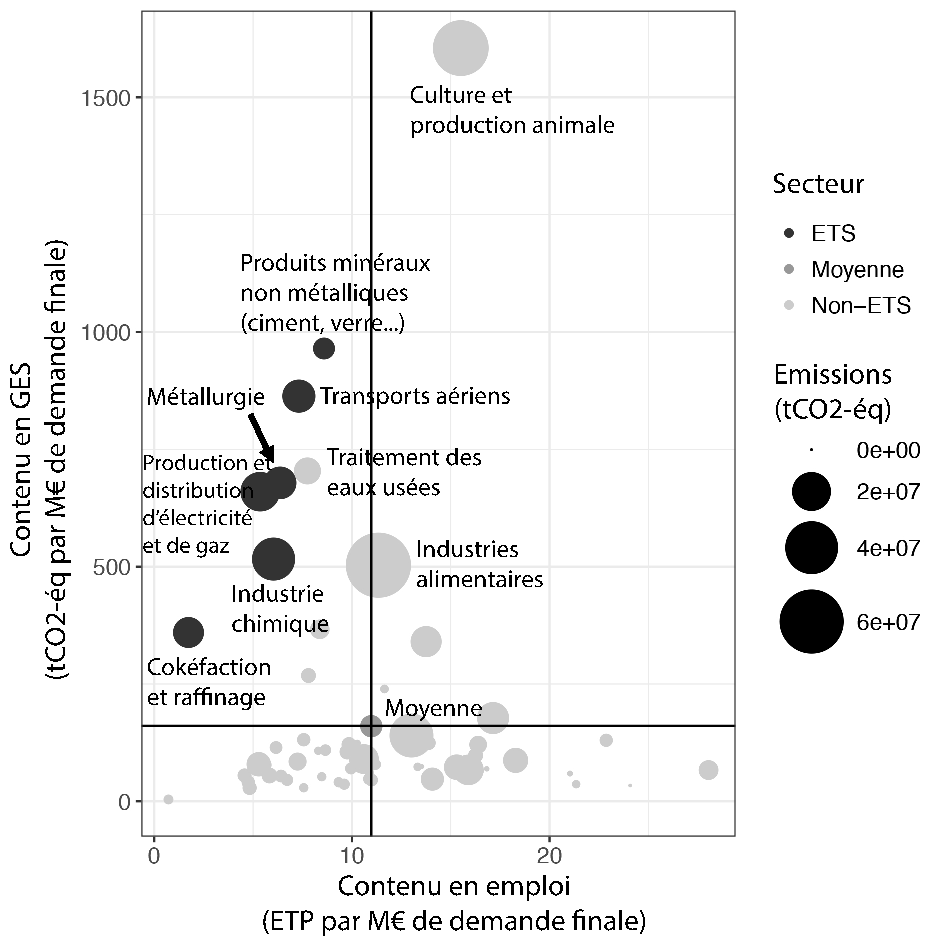
\includegraphics[height=11cm]{figures/GES_et_emplois/GES_emploi.pdf}
	\caption{Contenu en GES et en emploi des 64 branches de l'économie française. \\
		Sources : Calcul des auteurs à partir de données Eurostat.}
	\label{fig:ges_emploi}
	\captionsetup{justification=raggedright}
	\caption*{Lecture : la branche « Culture et production animale » de l’INSEE génère en moyenne 15,5 ETP et 1 600 tonnes d’équivalent-CO\textsubscript{2} par million d’euros de demande finale. La taille du cercle est proportionnelle à la quantité totale de gaz à effet de serre émise de façon directe et indirecte par la demande finale adressée à chaque branche. Le gris foncé indique les branches soumises à l’EU ETS.
		
		Les émissions directes des ménages, qui consistent essentiellement dans le transport terrestre privé et l’utilisation de gaz et de fioul pour le chauffage, l’eau chaude sanitaire et la cuisson, ne sont pas représentées ici car elles ne peuvent pas être analysées avec la même méthode. Une représentation incluant ces émissions est disponible dans l’annexe \ref{app:emissions_menages}. Les émissions considérées sont celles réalisées sur le territoire français, conformément aux engagements internationaux de la France ; les émissions liées aux importations ne sont pas incluses.}
\end{figure}

Les données publiées par Eurostat permettent d’effectuer le même croisement entre émissions et emploi, pour tout pays de l’Union Européenne. Ce travail a été réalisé pour l’Union européenne dans son ensemble, pour la même année (cf. annexe \ref{app:ges_emploi_EU}). On remarque une grande similitude avec les résultats pour la France, à part pour la branche électricité, gaz et vapeur, qui est beaucoup plus émettrice de GES au niveau européen qu'au niveau français, du fait de la forte part de nucléaire et d’hydraulique en France.


\subsection{Décomposition du contenu en emploi par branche}

\subsubsection{Remarques générales}

Le tableau \ref{tab:decompo_ce} montre le résultat de notre méthode pour les 60 branches de l’économie française (sur 64) auxquelles il est possible de l’appliquer. 
De façon générale, les branches industrielles présentent un contenu en ETP inférieur à la moyenne. Si les salaires élevés représentent souvent plus du tiers de ce bilan négatif, les importations élevées et/ou la faible part du travail jouent généralement dans le même sens et expliquent le reste. 
A l’inverse, l’agriculture (branche « culture et production animale ») et les services sont caractérisés par des salaires plus faibles, une forte part du travail et des importations faibles. 
Pour l’agriculture, un trait distinctif est la présence de subventions importantes. Il convient donc de relativiser le contenu en emploi de cette branche, puisque financer ces subventions nécessite des prélèvements, avec un impact récessif dans d’autres branches de l’économie. 
L’autre effet significatif provient des salaires, plus faibles que la moyenne de l’économie. Si l’on calcule un contenu en emploi pour l’agriculture « corrigé » en excluant les effets des taxes et subventions, le résultat s’avère en fait deux fois moins favorable à l'emploi par rapport à la moyenne de l'économie : +2,4 ETP/M\euro~de demande finale si l'on exclut les effets des taxes et subventions , contre +4,6 ETP/M\euro~de demande finale avec taxes et subventions). 

A ce niveau d’agrégation, il n’est pas possible de déduire directement de ces chiffres une quantification de l’effet sur l’emploi de la transition énergétique. En effet, il est difficile de savoir si la demande adressée à de nombreuses branches augmentera ou diminuera, du fait de changements intrabranches. 
Prenons l’exemple de l’automobile : le report modal vers des modes de transports moins émetteurs, le développement du télétravail ou le covoiturage auront tendance à diminuer la production automobile, mais la réduction des émissions par véhicule.km impliquera un développement des véhicules hybrides et électriques qui augmentera le prix unitaire des voitures. 
On ne peut savoir \textit{a priori} si la demande finale augmentera ou diminuera. 

En revanche, une partie de la transition énergétique passera par des substitutions interbranches identifiables au niveau d’agrégation auquel nous travaillons. Une comparaison deux-à-deux des branches amenées à croître et de celles qui pourraient décroître, en termes de contenu en emploi et des facteurs explicatifs de ce dernier, apporte un éclairage utile sur les enjeux économiques et sociaux de la transition énergétique. 

En France, les deux premiers secteurs émetteurs de CO\textsubscript{2} sont les transports et le résidentiel tertiaire, avec 41\% et 25\% des émissions en 2015 \citep{Dussud2016}. 
Parmi les nombreuses options disponibles pour réduire ces émissions, deux grands leviers permettent de décarboner ces secteurs au moyen de substitutions interbranches
: pour le résidentiel-tertiaire, l’isolation des logements, qui génère une baisse d’activité dans les branches énergétiques, à commencer par la branche « Electricité et gaz » ; pour les transports, le report modal en faveur des transports en commun, au détriment de la voiture particulière.
Dans les deux parties suivantes, nous étudions ces substitutions interbranches afin de détailler leur impact sur l'emploi. 

\subsubsection{Premier exemple : réduire la consommation d'électricité et de gaz en isolant les bâtiments}

Le bâtiment représente plus de 45\% de l’énergie finale consommée en France en 2014 (Ministère de l’Energie, 2015). Réduire significativement la consommation d’énergie passe nécessairement par une isolation des bâtiments, donc par une augmentation de la demande adressée à la construction (branche F dans la nomenclature NACE rev.2), au détriment des branches fournissant l’énergie, essentiellement l’électricité et le gaz (branche D35). Il peut donc être intéressant de comparer ces deux branches. Bien sûr, un euro de demande finale dépensé dans la construction ne va pas réduire d’autant la demande d’électricité. L’idée est ici de comparer les effets d’une politique soutenant la branche électrique et gazière - avec par exemple les subventions aux énergies fossiles \citep{OCDE2015} - à ceux d’une politique encourageant l'isolation des bâtiments. 

\begin{figure}[!ht]
	\centering
	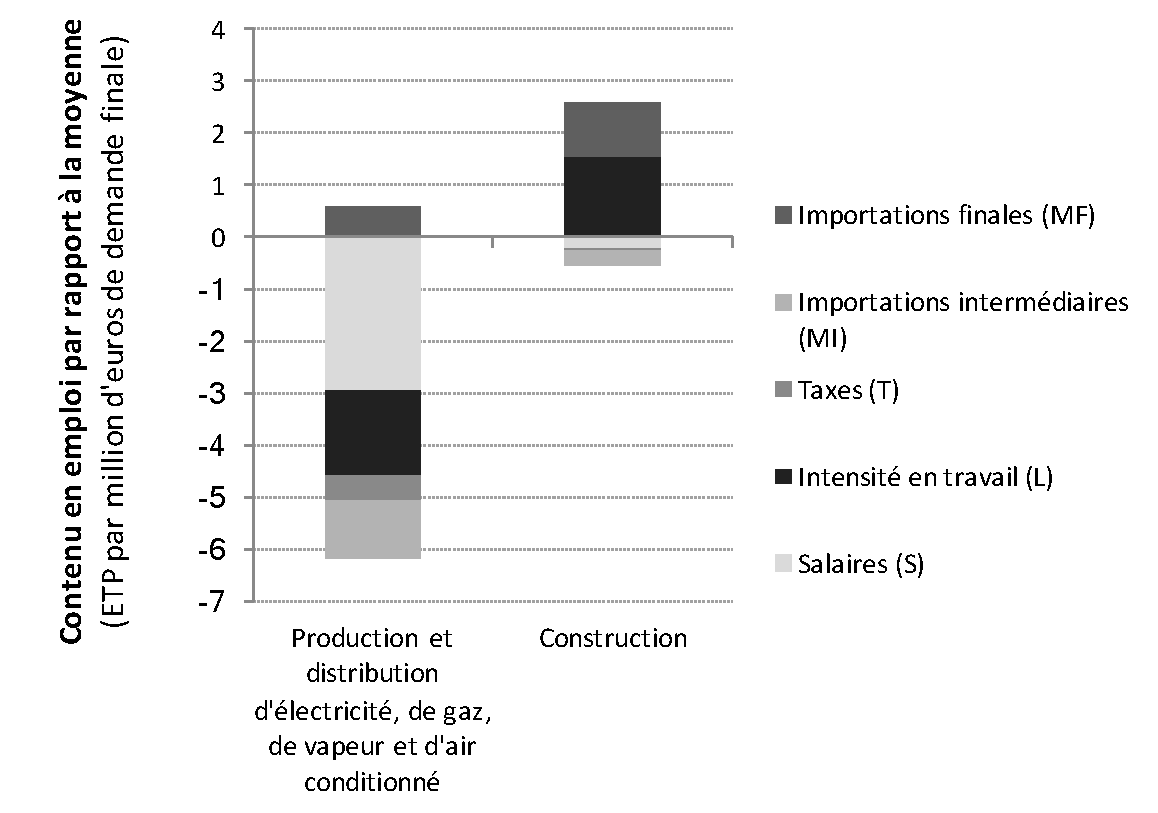
\includegraphics[width=12cm]{figures/comparaison1.pdf}
	\caption{Production et distribution d'électricité vs. Construction. \\ 
		Source : calculs des auteurs à partir de données Eurostat.}
	\label{fig:comparaison1}
	\captionsetup{justification=raggedright}
	\caption*{Lecture : ce graphique présente le contenu en ETP des deux branches F et D35 par rapport à la moyenne nationale, ainsi que la décomposition de cette différence. Allouer un million d'euros à la branche électricité-gaz génère 5,6 ETP de moins que la moyenne nationale. Cet effet négatif est essentiellement dû à des salaires élevés (- 3 ETP), à une faible part du travail dans la valeur ajoutée $L$ (- 1,6 ETP) et à des importations intermédiaires élevées (- 1,1 ETP). A l'inverse, la branche construction présente un contenu en emploi supérieur à la moyenne de 2 ETP par million d'euros de demande finale, principalement grâce à une forte part du travail dans la valeur ajoutée (+ 1,5 ETP) et un faible taux d'importations finales $MF$ (+ 1 ETP). 
	Réallouer un million d’euros de demande finale de la branche électricité-gaz vers la construction conduit à créer près de 7,6 ETP -- dont 3,1 ETP grâce à une plus grande part du travail dans la valeur ajoutée, et 1,3 ETP grâce à des importations plus faibles.}
\end{figure}

La figure \ref{fig:comparaison1} montre que la construction est moins intensive en émissions que la branche électrique et gazière. Et puisque l’isolation permet en plus de réduire les émissions directes des ménages (qui n’apparaissent donc pas dans la figure \ref{fig:ges_emploi}), le bilan total en GES est encore plus favorable à l’isolation. 
La figure \ref{fig:comparaison1} détaille les différences de contenu en emploi, et montre que la construction présente un contenu en emploi nettement plus important que la branche électricité. 
Cette différence provient essentiellement d'une plus forte part du travail dans la valeur ajoutée (à 42\%), des salaires plus faibles dans la branche construction (à 36\%) et d'importations plus faibles (à 17\%) dans la branche "Construction". Quant aux taxes et subventions, elles ne jouent qu’un rôle mineur (5\%). 
Une politique visant à promouvoir les économies d’énergies via l’isolation des bâtiments parait donc potentiellement génératrice d’emplois, et cela n’est dû qu’en partie à la faiblesse relative des salaires dans cette branche. 
Ces bilans en ETP ne tiennent pas compte des effets de friction temporaires, de l’inertie des migrations interbranches des employés \citep{Duhautois2005} ni de tous les ajustements sur le marché des biens et du travail. Mais ils fournissent une indication au premier ordre de l’effet sur l’emploi d’une réallocation de la demande finale.

\subsubsection{Deuxième exemple : réduire la consommation de carburant grâce aux  transports en commun}

Les transports en commun terrestres consomment moins de carburant et émettent moins de CO\textsubscript{2} que les véhicules particuliers, mais qu’en est-il de leur contenu en emploi ? Une telle substitution implique une modification de la demande adressée à différentes branches, et les transports en commun ne sont pas distingués du fret routier et ferroviaire à ce niveau de désagrégation. 
Cependant, une comparaison entre les branches H49 « transports terrestres et transports par conduite » et C19 « cokéfaction et raffinage » (figure \ref{fig:comparaison2}) fournit un premier éclairage. Une moindre utilisation des véhicules particuliers va réduire l’activité dans le raffinage de pétrole. Et la réallocation d’un million d’euros d’une branche à l’autre permet de créer 12 ETP. Hors effet de salaires et de taxes (qui pénalisent la branche C19), la différence s’élève encore à 8 ETP.

\begin{figure}[!ht]
	\centering
	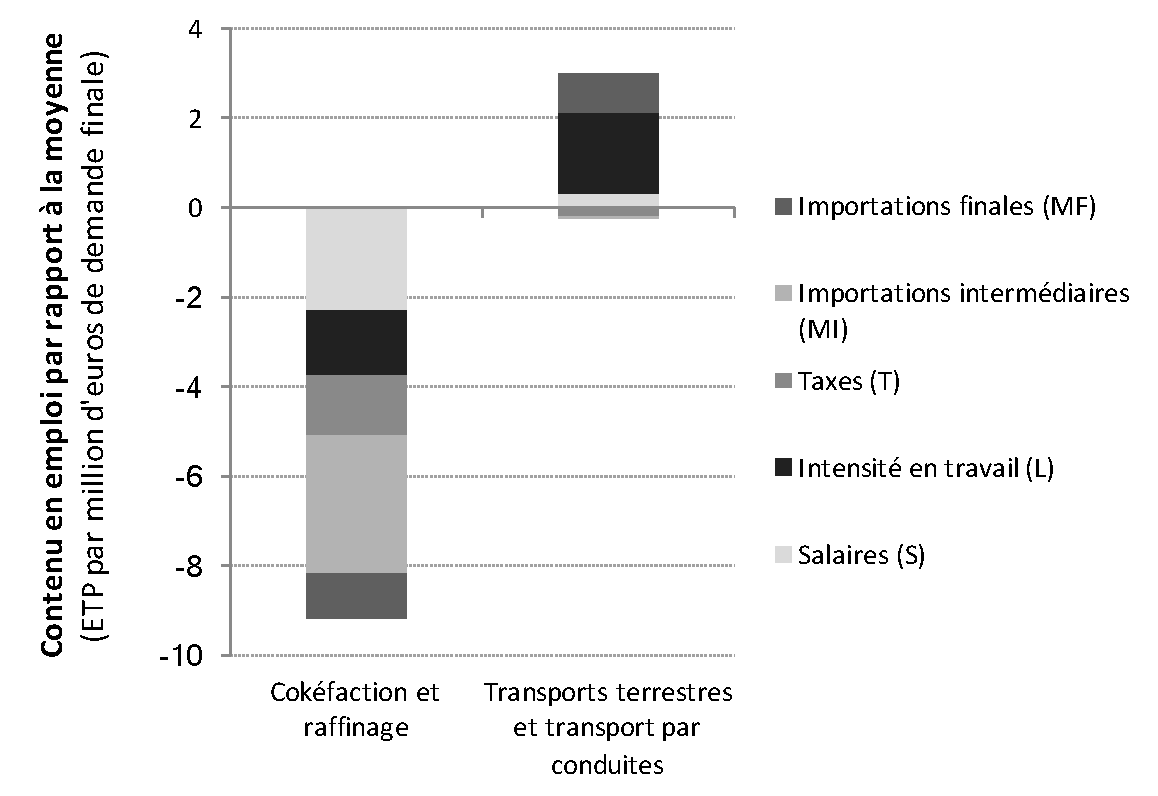
\includegraphics[width=12cm]{figures/comparaison2.pdf}
	\caption{Cokéfaction et raffinage vs. Transports terrestres. \\
		Source : calculs des auteurs à partir de données Eurostat.}
	\label{fig:comparaison2}
	\captionsetup{justification=raggedright}
	\caption*{Le faible contenu en emploi de la branche "Cokéfaction" par rapport à la moyenne s'explique essentiellement par de fortes importations intermédiaires (-3 ETP) et finales (- 1 ETP), ainsi que par de forts salaires (- 2,3 ETP) et la faible intensité en travail (-1,4 ETP). L'impact des taxes est ici marqué (-1,3 ETP). A l'inverse, la branche "Transports terrestres" présente un contenu en emploi supérieur à la moyenne, essentiellement grâce à un forte intensité en travail (+ 1,8 ETP) et de faibles importations finales (+ 0,9 ETP).}
\end{figure}

Cette comparaison ne prend pas en compte les effets dynamiques à plus long terme, par exemple la réduction de l’activité des producteurs d’automobiles. Mais elle fournit une explication des mécanismes de court terme. La décomposition peut également donner une intuition des mécanismes à l’œuvre dans les modèles macroéconomiques. Dans notre exemple, on peut s'attendre à un effet positif sur l'emploi provenant hausse de la production locale au détriment des importations et d'une plus forte demande de travail provenant de la part plus importante du travail dans le processus de production.


\section{Conclusion et discussion}

Nous calculons le contenu en emploi et le contenu en GES de 64 branches de l’économie française. 
Ces mesures sont utiles pour étudier des politiques publiques jouant sur la demande. 
Par exemple, améliorer l’efficacité énergétique dans le bâtiment diminue la demande d’énergie et augmente la demande des activités améliorant cette efficacité. Nos calculs fournissent une première approximation de cet effet.

Cependant, l’analyse agrégée que nous avons menée en distinguant 64 branches masque des disparités intra-branches. Prenons l’exemple de la production d’électricité : celle-présente un contenu en émissions de GES et en emploi très différents selon que l’électricité est produite à partir de charbon ou de sources renouvelables. 
Or la branche « production d’électricité et de gaz » du TES agrège ces différentes sources.

Pour obtenir des résultats plus fins, il est possible d’appliquer la même méthodologie à une branche en particulier, en détaillant des sous-branches. 
Par exemple, on pourrait distinguer les différentes filières de production d’électricité : photovoltaïque, éolien, nucléaire, gaz, charbon, etc. 
Une difficulté serait alors de reconstituer les données, car les agences de statistiques ne fournissent pas des données clés en main pour ce niveau de désagrégation. 
Pour chaque filière, il faudrait alors déterminer la production totale, le nombre d’emplois directs et une décomposition des consommations intermédiaires (donc de la chaîne de valeur) afin de déterminer le contenu en emploi. 
Il faudrait également estimer les émissions directes, et réutiliser la décomposition des consommations intermédiaires pour déterminer le contenu en GES (par exemple en se basant sur les données \citet{InNumeri2016} pour les emplois et ceux de \citet{Lehr2008} pour les consommations intermédiaires).

Par ailleurs, la réallocation d’un million d’euros de demande finale d’une branche vers une autre ne va pas générer un nombre d’emplois égal à la différence de leurs contenus en emploi. 
En effet, ce déplacement va entraîner d’autres effets et des ajustements sur les marchés du travail et des biens, qui ne sont pas pris en compte par notre approche comptable. 
Cette dernière ne cherche donc aucunement à se substituer aux autres analyses existantes, en particulier aux analyses d’équilibre général.

Cependant, notre analyse descriptive peut fournir une indication quant au sens, positif ou négatif, des évolutions entrainées par l’évolution de la demande – tant sur l’emploi que sur les émissions de gaz à effet de serre. 
Cette évolution de la demande finale peut être générée par des mécanismes fiscaux incitatifs. 
Par exemple, taxer le carbone peut encourager l’utilisation de transports en commun. 
Il serait également possible d’inclure l’aspect intensif en travail pour définir les aides d’Etat et orienter les choix technologiques (par exemple l'isolation des logements est certainement plus intensive en travail que la capture et le stockage géologique du CO\textsubscript{2}). 
Enfin, une autre option consiste en un investissement direct de l’Etat, par exemple dans les transports en commun.

En outre, nos résultats concordent avec les analyses en équilibre général qui ont été menées en France lors du débat national sur la transition énergétique. Ils permettent de mieux comprendre les mécanismes entrant en jeu dans les modèles d’équilibre général et les phénomènes de double dividende environnement-emploi observés dans de nombreuses simulations menées à l’aide de ces modèles.

Nos résultats confirment qu’il est essentiel de comprendre la composition du contenu en emploi pour donner un sens à cette mesure. 
Ainsi, l’agriculture semble de prime abord présenter un contenu en emploi bien plus élevé que la moyenne de l’économie. Mais la présence de subventions explique la moitié de cette différence positive par rapport à moyenne, et ces subventions vont nécessiter des prélèvements grevant l’activité dans d'autres branches. 
La méthodologie que nous présentons permet de calculer un contenu en ETP hors effet des taxes et des subventions. En outre, identifier la part des différences de salaire dans les différences de contenu en emploi entre branches est utile pour juger de l’intérêt de certaines substitutions interbranches d’un point de vue social.

Enfin, nous montrons que de nombreuses branches fortement émettrices de gaz à effet de serre sont peu intensives en emploi. C’est notamment le cas des branches incluses dans l’EU ETS. Il semble donc qu’il puisse exister un potentiel pour réussir une transition énergétique qui réduise les émissions tout en favorisant les branches à fort contenu en emploi.




\phantomsection
\printbibliography[heading=subbibintoc]
\begin{subappendices}
	\section*{Annexe}

\phantomsection % to make sure the clickable link points to the right page
\addcontentsline{toc}{section}{Annexe} % adds this label to the ToC

\subsection{Tableau de décomposition en emploi}
\label{app:tableau_ce}

\begin{small}
\begin{longtable}{m{1.3cm}m{5.7cm}m{1cm}rrrrr} %m aligns in the middle vertically
	\hline
	Code NACE & Intitulé & Contenu en ETP & $\Delta MF$ & $\Delta MI$ & $\Delta T$ & $\Delta L$ & $\Delta N$ \\ 
	\hline
	A01 & Culture et production animale, chasse et services annexes & 15,51 & -1,37 & -0,82 & 2,20 & -1,78 & 6,33 \\ 
	\hline
	A02 & Sylviculture et exploitation forestière & 11,64 & 0,46 & 0,08 & 0,55 & -0,79 & 0,38 \\ 
	\hline
	A03 & Pêche et aquaculture & 11,65 & -3,55 & -0,99 & -0,73 & 3,36 & 2,63 \\ 
	\hline
	C10-C12 & Industries alimentaires; fabrication de boissons et de produits à base de tabac & 11,34 & -0,69 & -0,19 & 0,06 & 0,28 & 0,94 \\ 
	\hline
	C13-C15 & Fabrication de textiles, industrie de l'habillement, du cuir et de la chaussure & 4,58 & -5,82 & -1,92 & -0,26 & 0,73 & 0,89 \\ 
	\hline
	C16 & Travail du bois et fabrication d'articles en bois et en liège, à l'exception des meubles; fabrication d'articles en vannerie et sparterie & 10,28 & -2,01 & -0,66 & -0,18 & 1,30 & 0,88 \\ 
	\hline
	C17 & Industrie du papier et du carton & 7,80 & -0,61 & -1,47 & -0,64 & 0,55 & -0,97 \\ 
	\hline
	C18 & Imprimerie et reproduction d'enregistrements & 13,03 & 1,08 & -0,66 & -0,50 & 2,28 & -0,11 \\ 
	\hline
	C19 & Cokéfaction et raffinage & 1,74 & -1,06 & -3,05 & -1,37 & -1,41 & -2,31 \\ 
	\hline
	C20 & Industrie chimique & 6,03 & -0,21 & -1,81 & -0,73 & -0,16 & -2,00 \\ 
	\hline
	C21 & Industrie pharmaceutique & 5,25 & -2,60 & -0,93 & -0,42 & -0,31 & -1,43 \\ 
	\hline
	C22 & Fabrication de produits en caoutchouc et en plastique & 7,55 & -1,82 & -1,50 & -0,43 & 0,78 & -0,42 \\ 
	\hline
	C23 & Fabrication d'autres produits minéraux non métalliques & 8,57 & -1,30 & -0,49 & -0,57 & 0,79 & -0,80 \\ 
	\hline
	C24 & Métallurgie & 6,36 & -0,64 & -1,92 & -0,67 & -0,26 & -1,08 \\ 
	\hline
	C25 & Fabrication de produits métalliques, à l'exception des machines et des équipements & 9,85 & -0,59 & -1,16 & -0,25 & 1,57 & -0,66 \\ 
	\hline
	C26 & Fabrication de produits informatiques, électroniques et optiques & 4,76 & -4,81 & -1,41 & -0,43 & 1,80 & -1,34 \\ 
	\hline
	C27 & Fabrication d'équipements électriques & 5,57 & -2,50 & -1,53 & -0,46 & 0,90 & -1,79 \\ 
	\hline
	C28 & Fabrication de machines et équipements n.c.a. & 7,25 & -1,70 & -1,33 & -0,36 & 0,50 & -0,80 \\ 
	\hline
	C29 & Industrie automobile & 5,28 & -2,94 & -1,65 & -0,73 & 0,66 & -1,00 \\ 
	\hline
	C30 & Fabrication d'autres matériels de transport & 5,82 & -0,59 & -2,47 & -0,83 & 0,79 & -2,03 \\ 
	\hline
	C31\_C32 & Fabrication de meubles; autres industries manufacturières & 6,73 & -4,76 & -0,64 & -0,18 & 1,07 & 0,30 \\ 
	\hline
	C33 & Réparation et installation de machines et d'équipements & 9,76 & 0,61 & -0,87 & -0,07 & 1,45 & -2,30 \\ 
	\hline
	D & Production et distribution d'électricité, de gaz, de vapeur et d'air conditionné & 5,35 & 0,61 & -1,14 & -0,47 & -1,65 & -2,94 \\ 
	\hline
	E36 & Captage, traitement et distribution d'eau & 8,29 & 0,79 & 0,32 & -0,24 & -3,12 & -0,40 \\ 
	\hline
	E37-E39 & Collecte et traitement des eaux usées, gestion des déchets, dépollution & 7,76 & 0,59 & -0,21 & 0,14 & 0,01 & -3,73 \\ 
	\hline
	F & Construction & 13,01 & 1,04 & -0,25 & -0,07 & 1,54 & -0,20 \\ 
	\hline
	G45 & Commerce et réparation d'automobiles et de motocycles & 16,38 & 1,18 & 0,03 & 0,32 & 2,04 & 1,87 \\ 
	\hline
	G46 & Commerce de gros, à l'exception des automobiles et des motocycles & 10,61 & 0,93 & 0,22 & -0,15 & 0,23 & -1,56 \\ 
	\hline
	G47 & Commerce de détail, à l'exception des automobiles et des motocycles & 18,27 & 1,25 & 0,47 & 0,15 & 1,80 & 3,66 \\ 
	\hline
	H49 & Transports terrestres et transport par conduites & 13,76 & 0,90 & -0,01 & -0,18 & 1,79 & 0,33 \\ 
	\hline
	H50 & Transports par eau & 8,39 & 0,71 & 0,11 & -0,73 & -1,48 & -1,17 \\ 
	\hline
	H51 & Transports aériens & 7,31 & -0,49 & -0,56 & -0,74 & 1,28 & -3,12 \\ 
	\hline
	H52 & Entreposage et services auxiliaires des transports & 8,48 & 0,40 & -0,04 & -0,23 & -0,80 & -1,79 \\ 
	\hline
	H53 & Activités de poste et de courrier & 21,04 & 0,76 & 0,61 & 1,03 & 5,38 & 2,32 \\ 
	\hline
	I & Hébergement et restauration & 17,14 & 1,20 & 0,32 & 0,27 & 1,97 & 2,44 \\ 
	\hline
	J58 & Édition & 9,94 & 1,44 & -0,16 & -0,05 & 0,87 & -3,11 \\ 
	\hline
	J59\_J60 & Activités cinématographique, vidéo, production de programmes de télévision, activités de programmation et de diffusion & 8,66 & 0,41 & -0,02 & 0,20 & -0,32 & -2,55 \\ 
	\hline
	J61 & Télécommunications & 6,42 & 0,49 & 0,09 & -0,21 & -2,69 & -2,20 \\ 
	\hline
	J62\_J63 & Programmation, conseil en informatique et autres services d'information & 9,62 & 0,66 & 0,20 & 0,11 & 1,89 & -4,19 \\ 
	\hline
	K64 & Activités des services financiers, hors assurance et caisses de retraite & 7,56 & 0,13 & 0,29 & -0,25 & -0,53 & -3,02 \\ 
	\hline
	K65 & Assurance & 10,99 & 0,70 & 0,51 & -0,73 & 1,55 & -1,98 \\ 
	\hline
	L & Activités immobilières & 4,82 & 0,62 & 0,22 & -0,44 & -4,07 & -2,45 \\ 
	\hline
	M69\_M70 & Activités juridiques et comptables; activités des sièges sociaux; conseil de gestion & 9,34 & 0,48 & 0,23 & -0,04 & 1,81 & -4,08 \\ 
	\hline
	M71 & Activités d'architecture et d'ingénierie; activités de contrôle et analyses techniques & 10,87 & 0,10 & -0,02 & 0,02 & 2,63 & -2,79 \\ 
	\hline
	M72 & Recherche-développement scientifique & 11,20 & 0,95 & -0,01 & 0,03 & 2,03 & -2,74 \\ 
	\hline
	M73 & Publicité et études de marché & 13,54 & 1,06 & 0,23 & -0,10 & 2,13 & -0,73 \\ 
	\hline
	M74\_M75 & Autres activités spécialisées, scientifiques et techniques, activités vétérinaires & 10,97 & 0,94 & -0,05 & 0,03 & 2,77 & -3,66 \\ 
	\hline
	N77 & Activités de location et location-bail & 6,16 & 0,69 & 0,22 & -0,05 & -3,92 & -1,72 \\ 
	\hline
	N78 & Activités liées à l'emploi & 24,07 & 1,42 & 1,08 & 1,18 & 6,54 & 2,91 \\ 
	\hline
	N79 & Activités des agences de voyage, voyagistes, services de réservation et activités connexes & 16,83 & 1,20 & 0,22 & -0,04 & 1,07 & 3,44 \\ 
	\hline
	N80-N82 & Enquêtes et sécurité, activités administratives, services et aménagement paysager & 16,48 & 1,14 & 0,16 & -0,01 & 2,38 & 1,86 \\ 
	\hline
	P & Enseignement & 15,30 & 1,12 & 0,66 & 1,05 & 3,16 & -1,64 \\ 
	\hline
	Q86 & Activités pour la santé humaine & 14,07 & 1,06 & 0,19 & 0,35 & 1,39 & 0,15 \\ 
	\hline
	R90-R92 & Activités créatives, artistiques et de spectacle; bibliothèques, archives, musées et autres activités culturelles; organisation de jeux de hasard et d'argent & 16,27 & 1,01 & 0,36 & 0,51 & 2,60 & 0,84 \\ 
	\hline
	R93 & Activités sportives, récréatives et de loisirs & 13,88 & 1,09 & 0,28 & 0,28 & 0,51 & 0,76 \\ 
	\hline
	S94 & Activités des organisations associatives & 22,86 & 1,42 & 0,65 & 0,52 & 4,40 & 4,93 \\ 
	\hline
	S95 & Réparation d'ordinateurs et de biens personnels et domestiques & 13,32 & 1,06 & -0,44 & 0,26 & 4,09 & -2,60 \\ 
	\hline
	S96 & Autres services personnels & 21,35 & 0,38 & 0,65 & 1,18 & 1,05 & 7,15 \\ 
	\hline
	\hline
	\caption{Tableau de décomposition en emploi \\ Source : calcul des auteurs à partir des données Eurostat} 
	\label{tab:decompo_ce}
\end{longtable}
\end{small}

\clearpage
\subsection{Décomposition du contenu en emploi en produit de facteurs}

Tout d'abord, on peut réécrire l'équation matricielle \ref{contenu_emploi} sous une forme d'indice. 
\begin{equation}
\forall i \quad ce_i = MF_i \cdot \sum_j Q^d_{ij} \cdot e_j
\label{decompo_initiale}
\end{equation}
en utilisant la définition $\pmb{Q^d} = (\pmb{I} - (\pmb{A^d})^T)^{-1}$. On peut ensuite décomposer plus avant les termes $e_j$ et $Q^d_{ij}$.

\subsubsection{Décompositon du vecteur \textit{\textbf{e}}}

Le nombre d'emploi par unité de production dans la branche $i$ peut se décomposer de la façon suivante :
\begin{equation}
\forall j \quad e_j = \frac{ETP_j}{P_j} = \frac{VA^d_j}{P_j} \cdot \frac{VA^{HT}_j}{VA^d_j} \cdot \frac{COMP_j}{VA^{HT}_j} \cdot \frac{ETP_j}{COMP_j}
\label{decompo_e}
\end{equation}

où 
\begin{itemize}
	\item $P^d_j$ la production intérieure dans la branche $j$ ;
	\item $VA^d_j$ est la valeur ajoutée intérieure générée dans la branche j. Il convient de noter que l’on considère ici la valeur ajoutée au sens de la comptabilité nationale, augmentée des « Impôts moins subventions sur les produits » (D21\_M\_D31) ;
	\item $VA^{HT}_j$ est la valeur ajoutée intérieure, déduction faite des taxes et subventions, générée dans la branche j. Pour obtenir  à partir de la valeur ajoutée brute , on déduit à la fois les « impôts moins subventions sur les produits » (D21\_M\_D31) et les « Autres impôts sur la production; impôts courants sur le revenu et le patrimoine; ajustement pour variation des droits des ménages sur les fonds de pension » (D29\_D5\_D8) ;
	\item $COMP_j$ sont les compensations salariales dans la branche j ;
	\item $ETP_j$ sont les ETP dans la branche j.
\end{itemize}
Cette écriture permet de faire apparaitre plusieurs ratios utiles à l'analyse. Le ratio $\frac{VA^{HT}_j}{VA^d_j}$ fait apparaitre l'importance des taxes dans la valeur ajoutée. On le nomme donc $T_j$. Le ratio $ \frac{COMP_j}{VA^{HT}_j}$ indique l'importance des rémunérations du travail par rapport aux rémunérations du capital. On l'indique par $L_j$. Enfin, le ratio $\frac{ETP_j}{COMP_j}$ est l'inverse du salaire, et indique donc le niveau de salaire. On le désigne par $N_j$.

\subsubsection{Décomposition de la matrice \textit{\textbf{Q\up{d}}}}
On peut ensuite décomposer la matrice $\pmb{Q^d}$.
\begin{align*}
\pmb{Q^d} =& (\pmb{I} - \pmb{A^d}^T)^{-1}  \\
\pmb{Q^d} =& (\pmb{I} - \pmb{A^t}^T + \pmb{A^m}^T)^{-1}  \\
\pmb{Q^d} =& (\pmb{I} - \pmb{A^t}^T)^{-1} \cdot (\pmb{I} + (\pmb{I} - \pmb{A^t}^T)^{-1}) \cdot \pmb{A^m})  \\
\pmb{Q^d} =& \pmb{Q^t}  \cdot (\pmb{I} + (\pmb{I} - \pmb{A^t}^T)^{-1}) \cdot \pmb{A^m})  \\
\end{align*}
où $^T$ représente l'opérateur de transposition matricielle. 
Cette dernière ligne montre bien que la production domestique est influencée par la fonction de production, donnée par la matrice $\pmb{A^t}$,
et par les taux d'importations, donnés par $\pmb{A^m}$. Cependant, pour notre décomposition, nous avons besoin d'un produit. En utilisant le produit d'Hadamard, qui multiplie terme à terme deux matrices, on définit la matrice 
$\pmb{MI}$ telle que : $\pmb{Q^d} =(\pmb{I} - \pmb{A^t}^T)^{-1} * \pmb{MI}$
Autrement dit, il s'agit d'une matrice telle que 
\begin{equation}
\forall i,j \quad Q^d_{ij} = Q^t_{ij} \cdot MI_{ij} 
\label{decompo_qd}
\end{equation} 

\subsubsection{Décomposition totale}
En injectant les équations \ref{decompo_e} et \ref{decompo_qd} dans l'équation \ref{decompo_initiale}, on obtient donc une formule globale : 

\begin{equation}
\forall i \quad ce_i = MF_i \cdot \sum_j  Q^t_{ij} \cdot MI_{ij} \cdot \frac{VA^d_j}{P_j} \cdot \frac{VA^{HT}_j}{VA^d_j} \cdot \frac{COMP_j}{VA^{HT}_j} \cdot \frac{ETP_j}{COMP_j}
\end{equation}

La dernière étape consiste à combiner $Q^t_{ij}$ et le ratio $\frac{VA^d_j}{P_j}$. L'idée est d'obtenir ainsi la valeur ajoutée par unité de demande finale. Nous le faisons car ce ratio nous semble plus significatif. On pose donc $V_{ij} = Q^t_{ij} \cdot \frac{VA^d_j}{P_j}$, soit, en termes matriciels, $\pmb{V} = \pmb{Q^t} \cdot \widehat{\pmb{vap}}$, avec $vap_j = \frac{VA^d_j}{P_j}$.

Ainsi, on obtient la forme décomposée finale du contenu en emploi : 
\begin{equation}
\forall i \quad ce_i = \sum_j CE_{ij} = \sum_j MF_i \cdot V_{ij} \cdot MI_{ij} \cdot T_j \cdot L_j \cdot N_j
\label{decompo_ce}
\end{equation}
où
\begin{itemize}
	\item $MF_i = \frac{D^d}{D^t}$ est le taux de demande intérieure dans la demande finale totale ;
	\item $V_{ij} = Q^t_{ij} \cdot \frac{VA^d_j}{P_j}$ est la valeur ajoutée intérieure par unité de production ;
	\item $MI_{ij} = \frac{Q^d_{ij}}{Q^t_{ij}}$ indique le taux d'importations intermédiaires ;
	\item $T_j = \frac{VA^{HT}_j}{VA^d_j}$ le taux de taxes et subventions (« Autre impôts sur la production », code D29\_M\_D39 et « Impôts moins subventions sur les produits », code D21\_M\_D31) dans la valeur ajoutée augmentée des « Impôts moins subventions sur les produits »;
	\item $L_j = \frac{COMP_j}{VA^{HT}_j}$ représente la part des rémunérations du travail dans la valeur ajoutée moins les « autres impôts sur la production (D29\_M\_D39) ;
	\item $N_j = \frac{ETP_j}{COMP_j}$ est égal à l’inverse du salaire. Il mesure donc le niveau des salaires.
\end{itemize}

Cette suite de ratios suit la logique illustrée par la figure \ref{fig:schema_decompo} : une demande finale totale va susciter d’une part des importations de produits finaux, et d’autre part une demande intérieure qui est adressée à la production intérieure. La demande intérieure suscite une production dans d’autres branches du fait des consommations intermédiaires, et donc la création de valeur ajoutée dans chaque branche. Une partie de cette valeur ajoutée est captée à l’étranger à cause des importations de produits intermédiaires. Dans la valeur ajoutée intérieure restante, une partie sert à payer des taxes ou provient de subventions. Enfin, la valeur ajoutée hors taxes et subventions rémunère le capital et les compensations salariales. Ces dernières servent à employer des travailleurs.

On a ainsi pu décomposer le contenu en ETP comme somme de produits de ratios significatifs pour l’analyse. Nous pourrons ainsi répondre à des questions du type : le contenu en emploi de telle branche est-il élevé du fait de salaires faibles, du petit nombre d’importations, des taxes élevées… ?

\subsubsection{Deux remarques}

\emph{Remarque 1 : écriture matricielle}

Notons qu'en termes matriciels, l'équation \ref{decompo_ce} peut s'écrire : 

\begin{align*}
\pmb{ce} &=~\widehat{\pmb{mf}} \cdot \left( \pmb{V}  * \pmb{MI} \right) \cdot \widehat{ \pmb{t}} \cdot \widehat{\pmb{l}} \cdot~\pmb{n}  
\end{align*}
En faisant attention au fait que l'opérateur * indique ici le produit terme à terme d'Hadamard.\\

\emph{Remarque 2 : Pourquoi ne pas faire apparaitre la production ?}

L’utilisation des matrices de Leontief fait généralement apparaitre la production. 
Cependant, cette formulation présente un problème de corrélation avec l’autoconsommation des branches. 
En effet, toutes choses égales par ailleurs, une autoconsommation plus importante va augmenter la production par unité de demande finale (le terme P/D), mais diminuer la valeur ajoutée par unité de production (VA/P) ; en revanche, le ratio VA/D va rester constant (et donc, toutes choses égales par ailleurs, le nombre d’emplois). 
Ce problème de l’autoconsommation fait que la décomposition en deux termes donne des résultats très sensibles au choix – arbitraire – de la décomposition en branches de l’économie, ce qui n’est pas une propriété souhaitable. 
En outre, en menant les calculs avec les deux ratios, nous avons en effet constaté une corrélation très importante entre ces deux termes. 
Nous avons donc finalement choisi de ne pas faire apparaitre la production, car ce ratio supplémentaire complexifie l’analyse pour un gain faible en termes de compréhension.


\cleardoublepage
\subsection{Détermination de la moyenne}
\label{app:def_moyenne}

Pour mesurer l’écart du contenu en emploi de la demande finale entre une branche donnée et la moyenne de l’économie, nous allons considérer le contenu moyen en emploi en le définissant par :
\begin{equation}
\forall i \quad ce_{i,m} = \sum_j MF_m \cdot V_{ij,m} \cdot MI_{ij,m} \cdot T_m \cdot L_m \cdot N_m
\end{equation}

Avec :
\begin{itemize}
	\item $MF_m = \frac{\sum_j D^d_j}{\sum_j D^t_j} $  est égal à l’ensemble de la demande finale hors importations finales divisé par l’ensemble de la demande finale totale.
	\item $V_{ij,m} = Q^t_{ij,m} \cdot (\frac{VA^d}{P})_m$ est obtenu de manière plus indirecte, car il nécessite de définir la matrice $\pmb{Q^t_m}$ et un ratio moyen $(\frac{VA^d}{P})_m$. Pour le ratio moyen, on prend simplement $(\frac{VA^d}{P})_m = \frac{\sum_i VAI^d_i}{\sum_i P_i}$.
	Pour la matrice $Q^t_m$, il faut distinguer le terme diagonal et les autres. On prend donc une valeur moyenne différente pour les deux termes : $\forall i \quad Q^t_{ii,m} = \text{moyenne } {Q^t_{ii}}$ et $\forall i \neq j \quad Q^t_{ij,m} = \text{moyenne }{Q^t_{ij}}$
	\item Pour $MI_m$ on prend également la valeur moyenne en distinguant le terme diagonal : $MI_{ii,m} = \frac{Q^d_{ii,m}}{Q^t_{ii,m}}$ et $\forall i \neq j \quad MI_{ij,m} = \frac{Q^d_{ij,m}}{Q^t_{ij,m}}$
	\item $T_m = \frac{\sum_j VA^{HT}_j}{\sum_j VA^d_j}$ C’est la somme des valeurs ajoutées augmentées des « Impôts moins subventions sur les produits » (D21\_M\_D31) et retranchées des taxes et subventions, divisé par la somme des valeurs ajoutées augmentées des « Impôts moins subventions sur les produits ».
	\item $L_m = \frac{\sum_j COMP_j}{\sum_j VA^{HT}_j}$. C'est la sommes des valeurs ajoutées nettes, afin d’obtenir la part moyenne des salaires et cotisations salariales dans la valeur ajoutée nette.
	\item $N_m = \frac{\sum_j ETP_j}{\sum_j COMP_j}$. On divise le nombre total d’ETP de l’économie par la somme des compensations salariales versées.
\end{itemize}
 
 
\clearpage

\subsection{Clé de ventilation et décomposition LMDI}
\label{app:ventilation_LMDI}

Ainsi, pour une branche donnée i, l’écart entre le contenu en ETP de cette branche et le contenu en ETP moyen vaut :

\begin{align}
\forall i \quad ce_i - ce_{i,m} &= \sum_j CE_{ij} - CE_{ij,m} \\
											&= \sum_j MF_i \cdot V_{ij} \cdot MI_{ij} \cdot T_j \cdot L_j \cdot N_j -  \sum_j MF_m \cdot V_{ij,m} \cdot MI_{ij,m} \cdot T_m \cdot L_m \cdot N_m 
\label{diff_ce}
\end{align}

On peut alors détailler la part de chacun de ces facteurs en utilisant des méthodes de décomposition d’index. Une dernière étape est toutefois nécessaire. En effet, le coefficient de valeur ajoutée ne nous parait pas un facteur d’explication au même titre que les autres. On comprend bien que le contenu en emploi puisse être plus élevé du fait d’importations finales (MF) ou intermédiaires (MI), de taxes (T), d’une forte part du travail dans la valeur ajoutée (L) ou de salaires faibles (N). Mais que signifie une forte valeur ajoutée par unité de demande finale ? On peut mieux voir l’effet de ce paramètre en observant la figure \ref{fig:schema_decompo}. 
Ce coefficient $V$ joue en fait le rôle de clé de ventilation : le contenu en emploi d’une branche sera élevé si qu’elle fait beaucoup appel à des branches présentant peu d’importations, des salaires faibles, etc.
Ce rôle peut être également vu si l’on cherche à comparer deux branches directement. Les $T_j$, $L_j$ et $N_j$ étant identiques, une méthode de décomposition d’index attribuerait tout leur apport via l’indice $V_{ij}$. Ce qui suit une certaine logique : étant donné les taxes, parts du travail dans la valeur ajoutée et salaires, toute la variation du contenu en emploi peut être expliquée par la répartition de la valeur qui est faite entre ces branches lors du processus de production. Afin de distinguer séparément l’effet de chacun des termes $T_j$, $L_j$ et $N_j$, il nous faut donc réécrire la formule précédente. Partant de l’idée que $V_{ij}$ joue le rôle de clé de répartition, nous la distribuons entre les quatre facteurs qui suivent. On décompose alors le contenu en ETP d’une branche $i$ sous la forme :
\begin{equation}
\forall i \quad ce_i = \sum_j MF_i \cdot (V_{ij}^{1/4} \cdot MI_{ij}) \cdot (V_{ij}^{1/4} \cdot T_j) \cdot (V_{ij}^{1/4} \cdot L_j) \cdot (V_{ij}^{1/4} \cdot N_j)
\label{realloc_v}
\end{equation}

Le contenu en emploi est ainsi décomposé sous la forme de quatre facteurs. On retrouve l’idée que le contenu en ETP d’une branche sera élevé si cette branche fait beaucoup appel, en termes de valeur ajoutée, à des branches aux importations faibles, aux taxes limitées, à des branches intensives en main-d’œuvre ou ayant des salaires faibles.

On peut alors comparer le contenu en ETP de chacune des branches i avec la moyenne. En combinant les équations \ref{diff_ce} et \ref{realloc_v}, et en appliquant la méthode LMDI (Logarithm Mean Divisia Index) de décomposition d’indice développée par \citet{Ang2005}, on peut transformer cette différence en somme de termes traduisant chacun l’apport d'un facteur :
\begin{equation}
\forall i \quad ce_i - ce_{i,m} = \Delta MF_i + \Delta MI_i + \Delta T_i +\Delta L_i + \Delta N_i
\end{equation}

Il est ainsi possible de déterminer l’impact des différents facteurs dans la composition et le niveau du contenu en ETP. On peut donc répondre à la question : pourquoi le contenu en emploi d’une branche est-il élevé ? Est-ce du fait d’importations finales ou intermédiaires faibles, de taxes faibles, d’une forte part du travail dans la valeur ajoutée, ou de salaires bas ?

\cleardoublepage

\subsection{Décomposition LMDI}
\label{app:decompo_LMDI}


Pour chaque branche i, nous avons réalisé une décomposition structurelle, c'est-à-dire une décomposition mobilisant les informations des tableaux entrées-sorties. L'originalité de l'approche est de chercher ici à comprendre les différences entre chaque branche et la moyenne de l'économie, plutôt que d'analyser une évolution temporelle. 

Plusieurs méthodes sont disponibles pour analyser l'impact de chaque terme dans la décomposition entre contenu en emploi d’une branche et contenu en emploi de la moyenne de l’économie présentée dans l'équation \ref{diff_ce}. Le choix de la méthode n'est jamais neutre, puisqu'il influe sur les résultats de la décomposition \citep{Hoekstra2003}. La méthode couramment employée est celle dite "LMDI" (Logarithm Mean Divisa Index) développée par \citet{Ang2004,Ang2005} et présentée comme la meilleure décomposition par le même auteur, notamment pour le fait qu’elle ne présente aucun terme résiduel. Cependant, nous utiliserons cette méthode principalement pour les raisons avancées par \citet{Muller} : le fait qu'aucun résidu apparaisse n'est pas la preuve d'une bonne méthode de décomposition, car ce résidu peut être distribué de façon arbitraire ou incorrecte et fausser les résultats ; en revanche la méthode LMDI semble fournir la meilleure décomposition pour un grand nombre de fonctions, et notamment pour les fonctions les plus usuelles.

En appliquant la méthode LMDI à la différence donnée par l'équation \ref{diff_ce} et en appliquant la réallocation donnée dans l'équation \ref{realloc_v}, on peut décomposer le contenu en emploi sous la forme : 
\begin{equation*}
\forall i \quad ce_i - ce_{i,m} = \Delta MF_i + \Delta MI_i + \Delta T_i +\Delta L_i + \Delta N_i
\end{equation*}

Où chaque terme représente la part d’un coefficient à l’évolution globale du contenu en emploi cei de la branche i, avec :
\begin{equation}
\renewcommand*{\arraystretch}{2}
	\left\{
	\begin{array}{ll}
	\Delta MF_i &= \sum_j w_{ij} \ln(\frac{MF_i}{MF_m}) \\
	\Delta MI_i &= \sum_j w_{ij} \ln( k_{ij} \cdot \frac{MI_{ij}}{MI_m}) \\
	\Delta T_i &= \sum_j w_{ij} \ln( k_{ij} \cdot \frac{T_j}{T_m}) \\
	\Delta L_i &= \sum_j w_{ij} \ln( k_{ij} \cdot \frac{V_{ij}}{V_m} \cdot \frac{L_j}{L_m}) \\
	\Delta N_i &= \sum_j w_{ij} \ln( k_{ij} \cdot \frac{V_{ij}}{V_m} \cdot \frac{N_j}{N_m}) \\
	w_i &= \frac{CE_{ij} - CE_{ij,m}}{\ln(CE_{ij}) - \ln(CE_{ij,m})} \\
	k_{ij} &= \left(\frac{V_{ij}}{V_{ij,m}} \right)^{1/4}
	\end{array}
	\right.
\end{equation}


où $CE_{ij}$ est le contenu en emploi dans la branche $j$ due à une demande finale adressée à la branche $i$. Autrement dit, c'est le nombre d'emploi créés dans la branche $j$ du fait d'une demande unitaire adressée à la branche $i$. Ce contenu en emploi correspond au terme d'indice $(i,j)$ dans la matrice $$\pmb{CE} =~\widehat{\pmb{mf}} \cdot (\pmb{I} - (\pmb{A^d})^T)^{-1} \cdot \widehat{\pmb{e}}$$

Comme mentionné précédemment, la méthode LMDI présente la particularité de distribuer les résidus entre les différents facteurs. Comme cette distribution reste arbitraire et inconnue, il convient de vérifier que la taille des résidus n’est pas trop importante. Pour ce faire, on compare la méthode LMDI à une autre méthode. Par exemple, en utilisant la méthode des trapèzes telle que définie par \citet{Muller}, on peut se faire une idée. On peut alors vérifier que les résidus sont de second ordre par rapport au terme principal pour toutes les branches pour lesquelles la méthodologie s’applique (c’est-à-dire toutes les branches sauf celles correspondant aux codes B, K66, L68A et T dans la nomenclature NACE Rév. 2).


\cleardoublepage
\subsection{Graphique au niveau de l'Union Européenne}
\label{app:ges_emploi_EU}

\begin{figure}[!h]
	\centering
	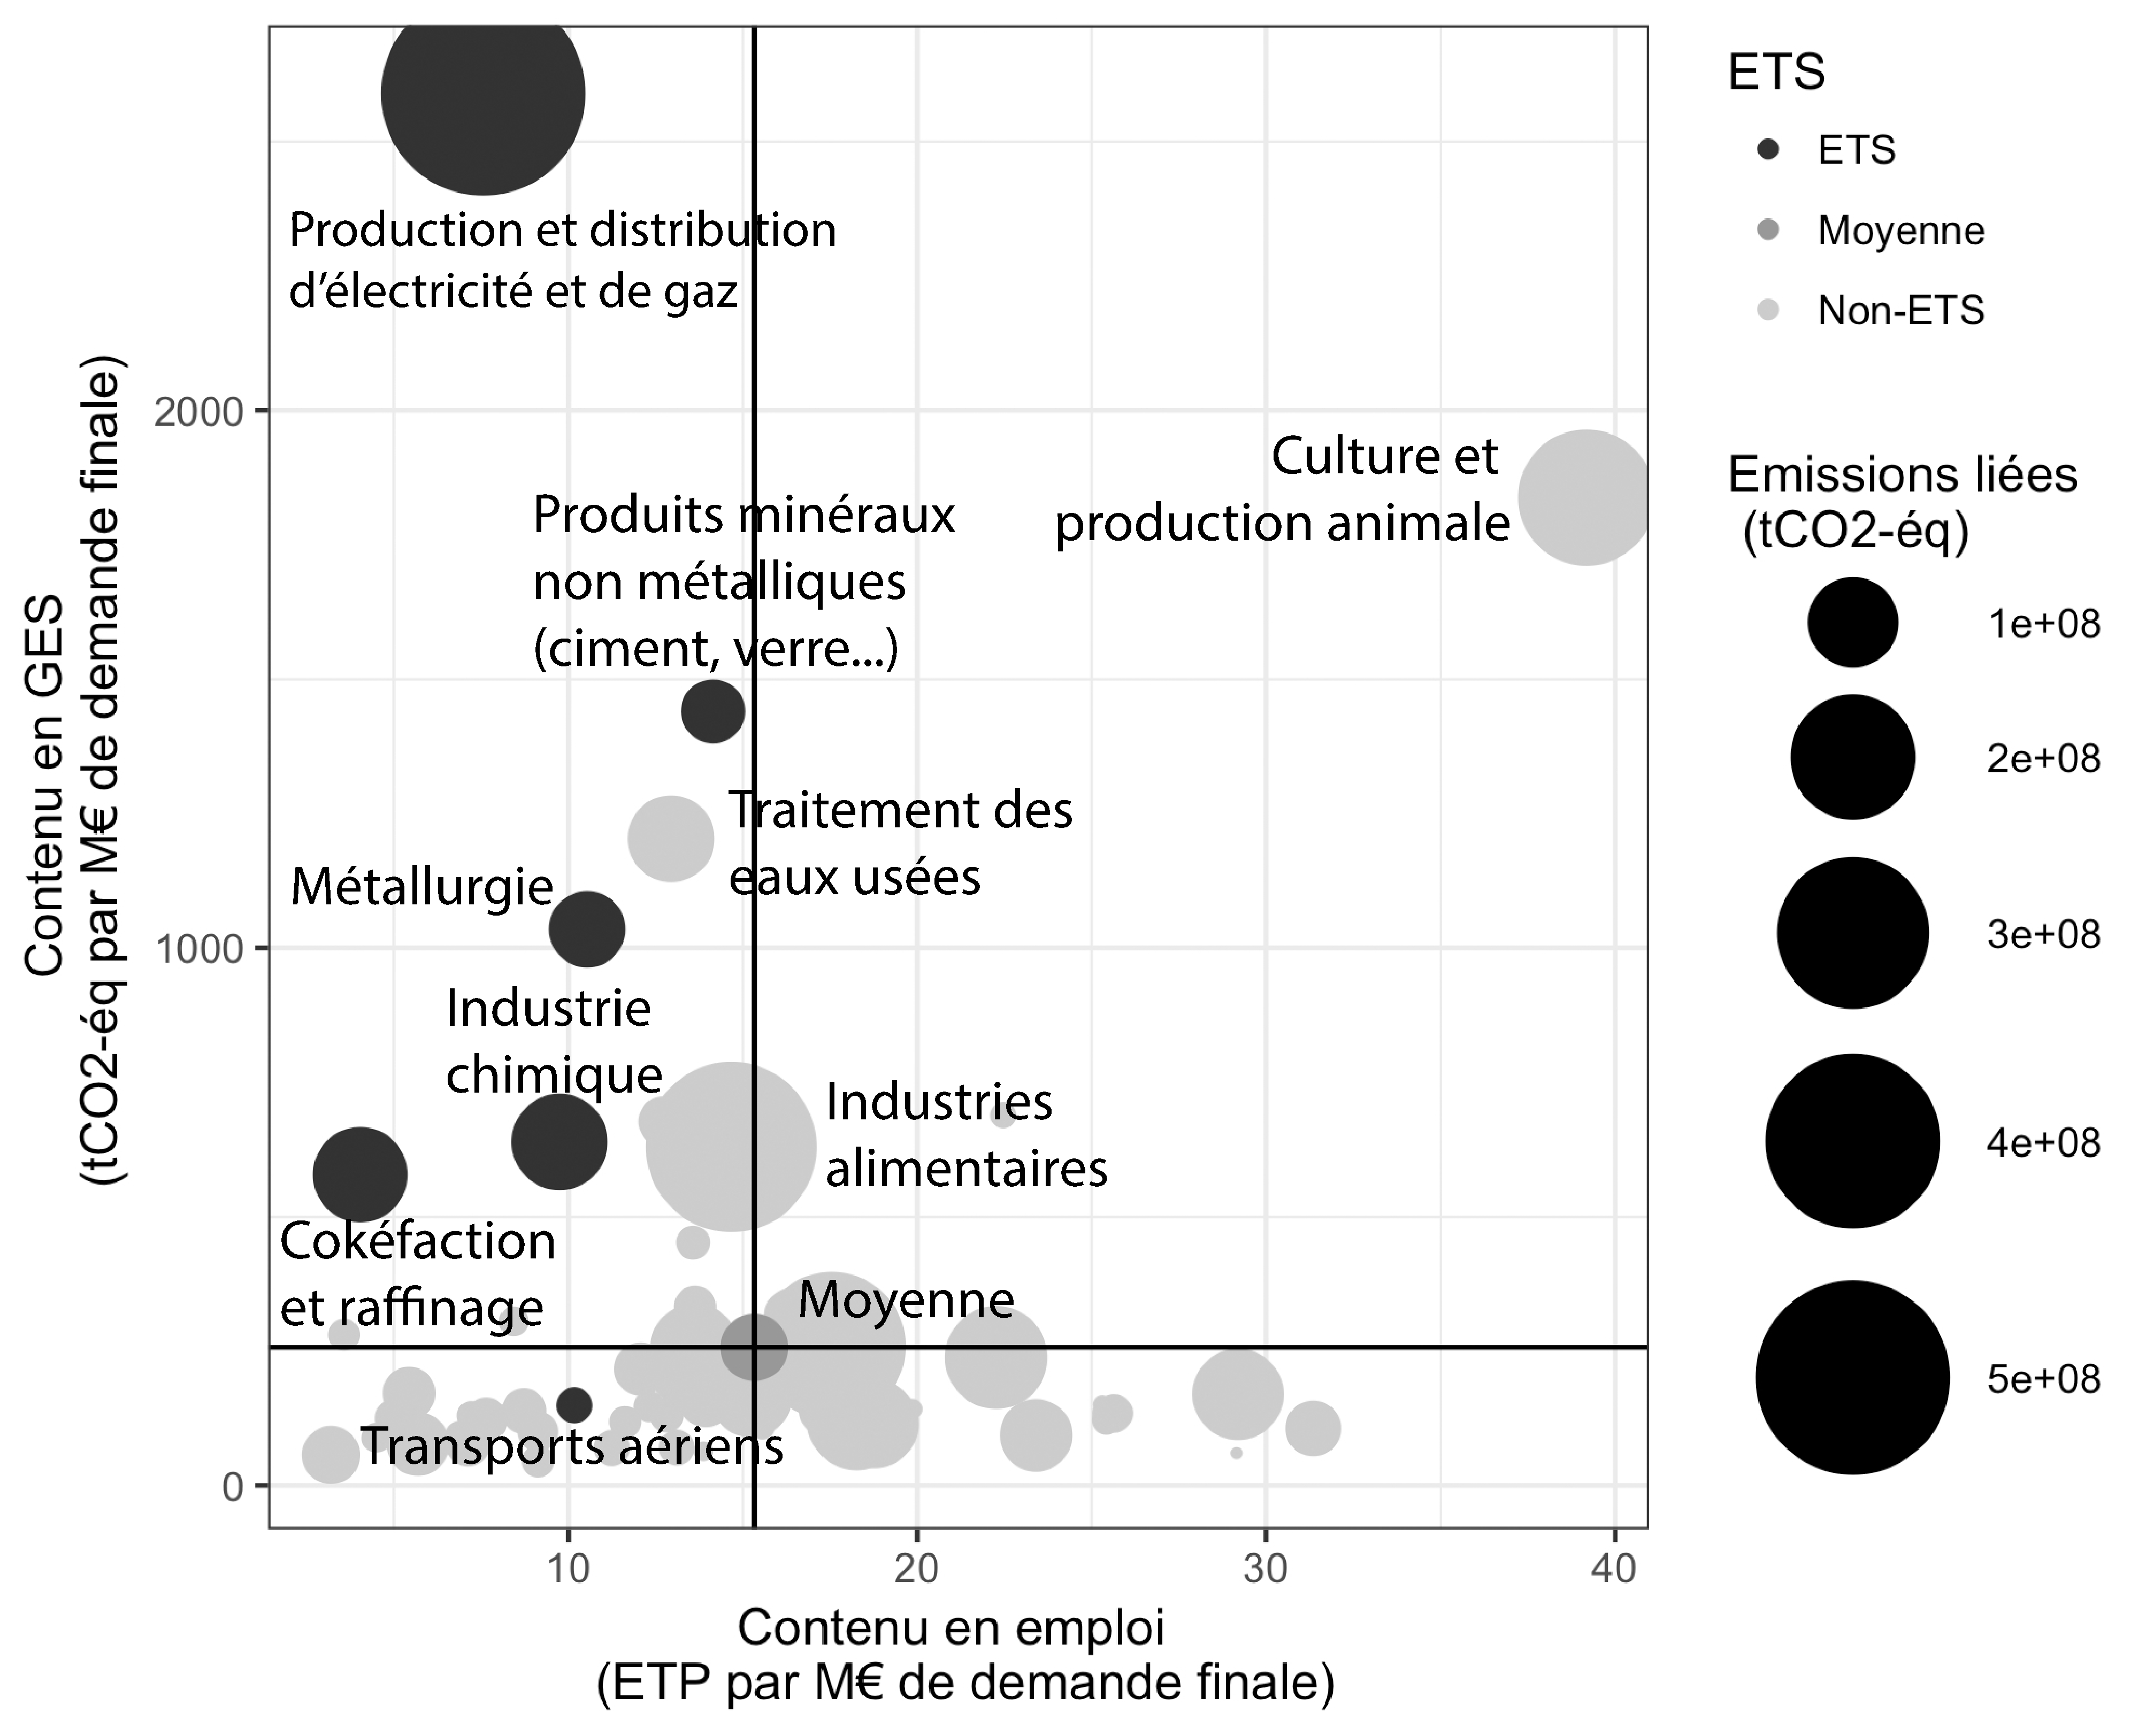
\includegraphics[height=11cm]{figures/GES_et_emplois/GES_emploi_EU.pdf}
	\caption{Contenu en GES et en emploi des 64 branches de l'économie européenne (Union des 27) \\
		Sources : Calcul des auteurs à partir de données Eurostat.}
	\label{fig:ges_emploi_EU}
	\captionsetup{justification=raggedright}
	\caption*{Lecture : ce graphique est identique à la figure \ref{fig:ges_emploi}, mais le périmètre est ici celui des 27 pays membres de l'Union Européenne. On note que la branche "Production et distribution d'électricité et de gaz" est ici beaucoup plus émettrice que pour la France. La présence de nucléaire et d'hydraulique en France explique en grande partie cette différence.}
\end{figure}


\clearpage
\subsection{Graphique incluant les émissions finales des ménages}
\label{app:emissions_menages}

\begin{figure}[!h]
	\centering
	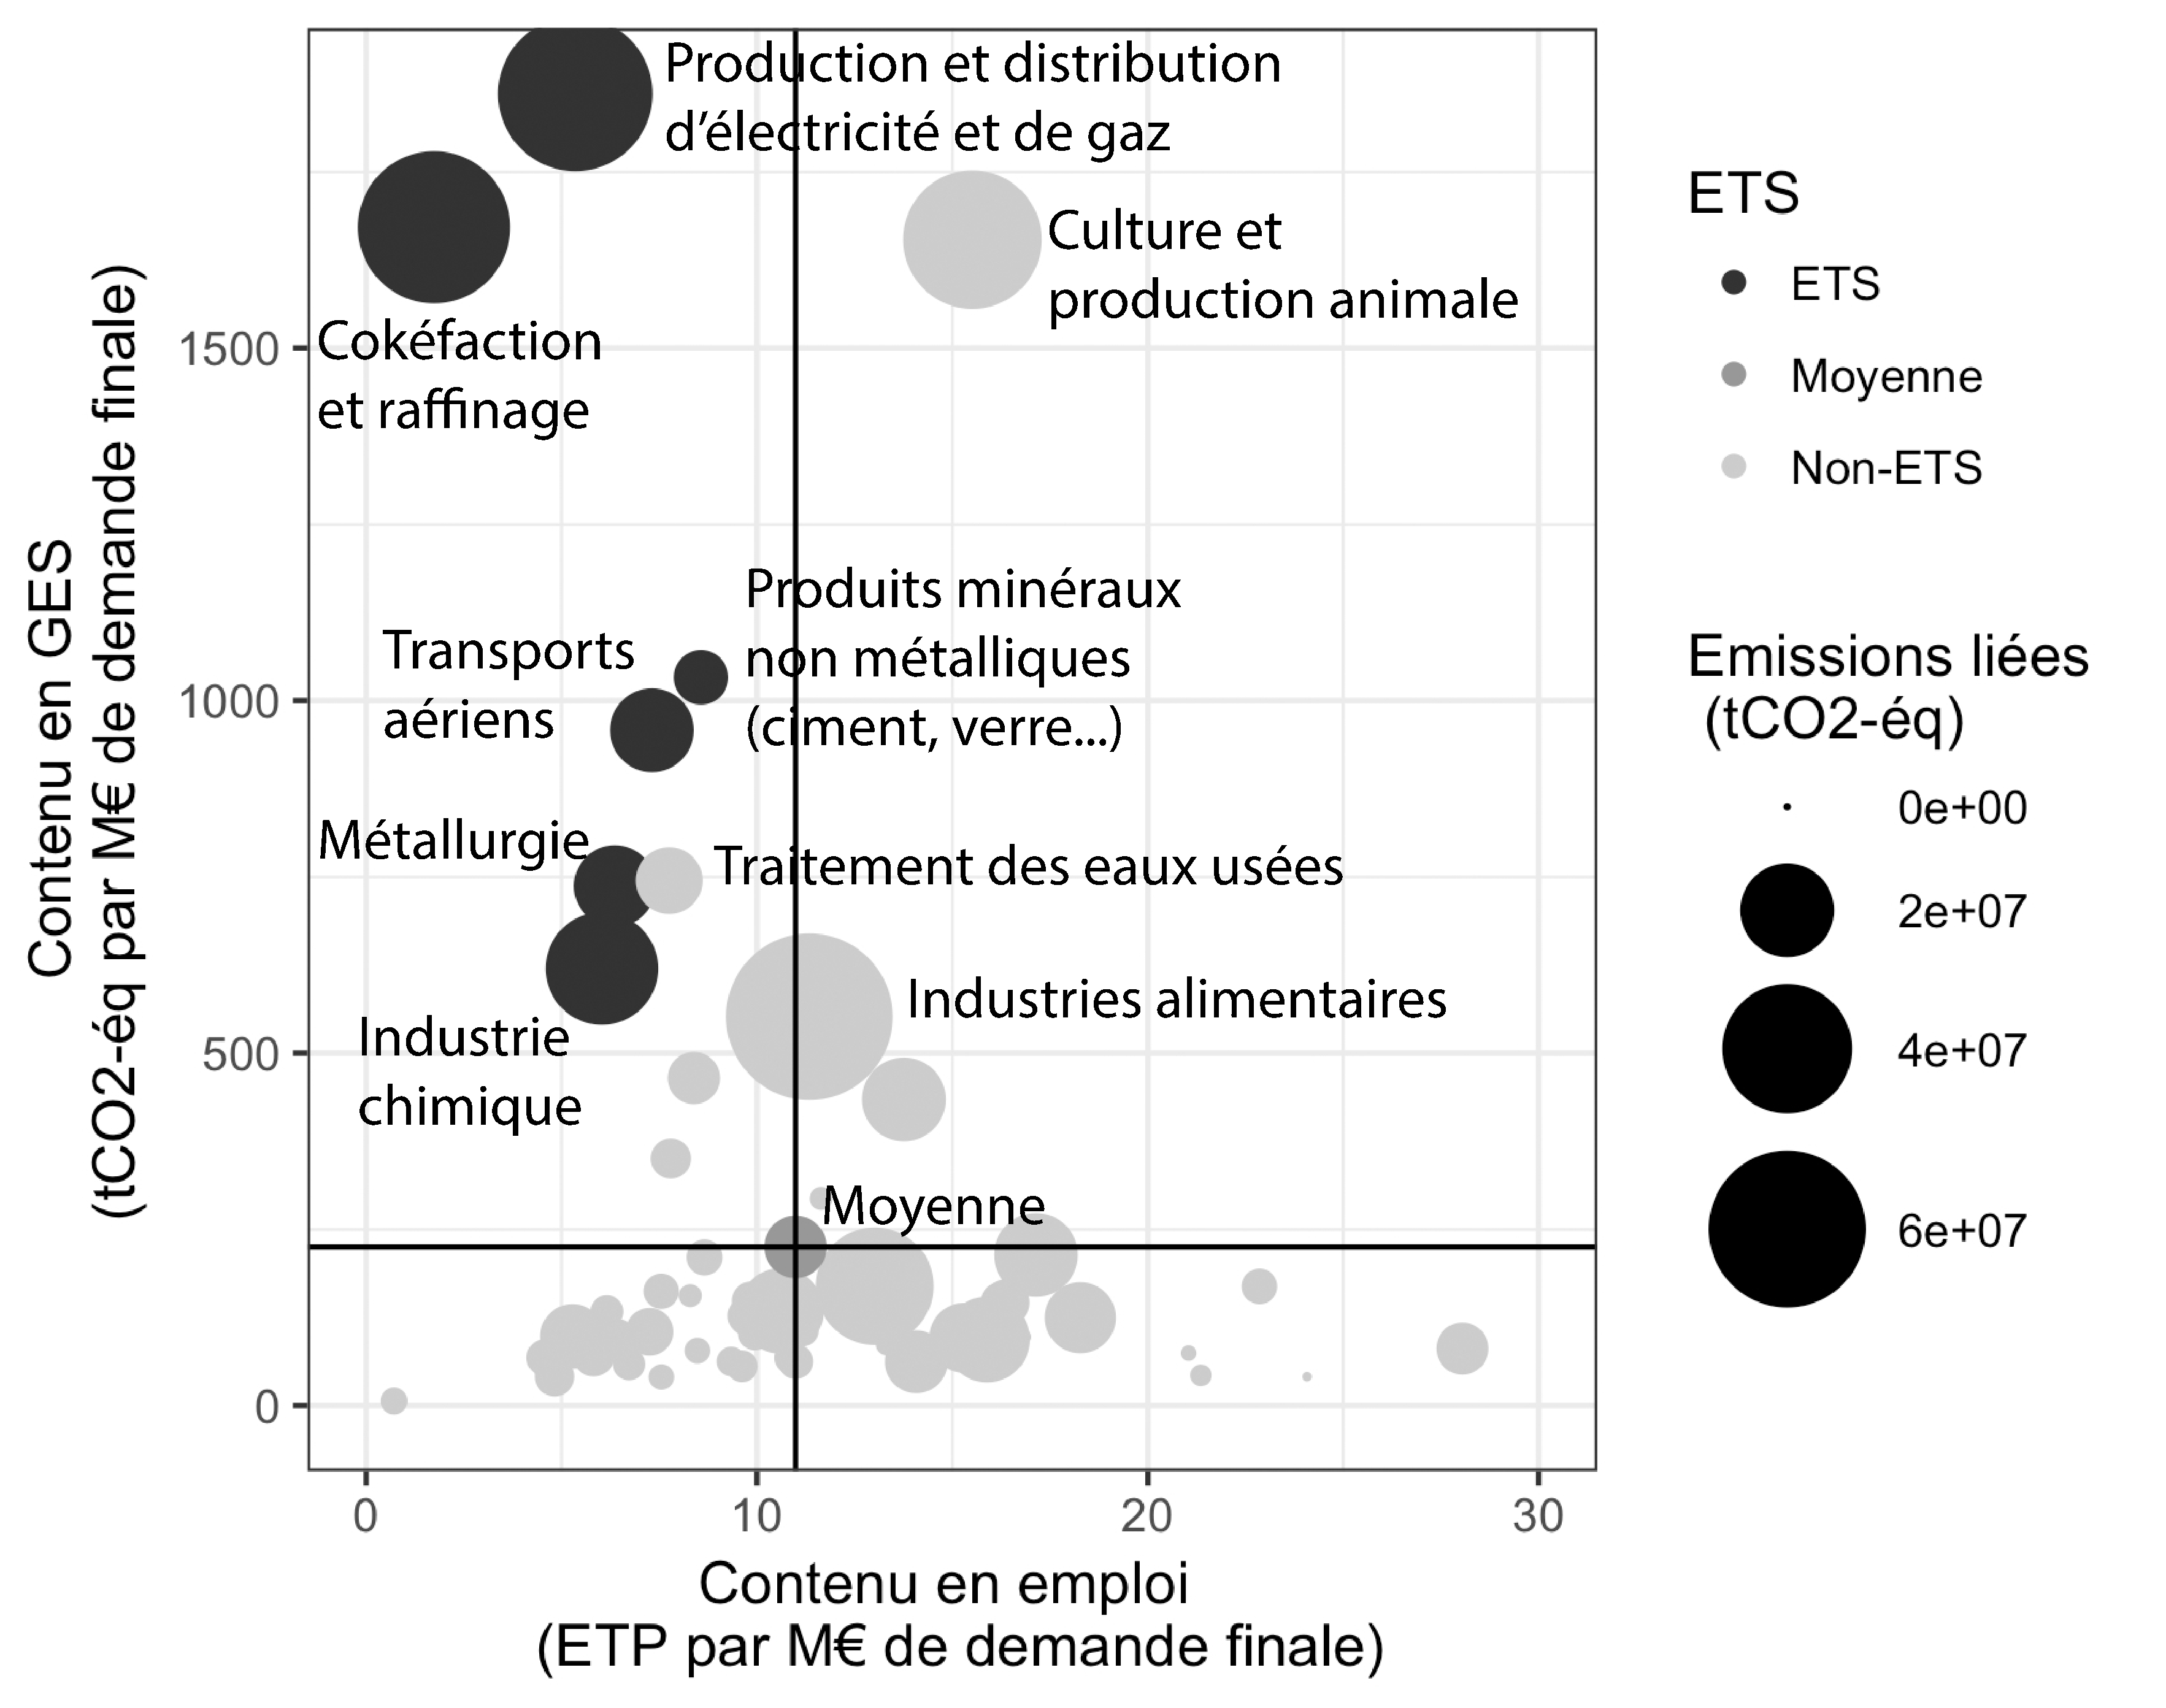
\includegraphics[height=11cm]{figures/GES_et_emplois/GES_menages_emploi.pdf}
	\caption{Contenu en GES et en emploi des 64 branches de l'économie française, en incluant les émissions finales \\
		Sources : Calcul des auteurs à partir de données Eurostat.}
	\label{fig:ges_menages_emploi}
	\captionsetup{justification=raggedright}
	\caption*{Lecture : Cette figure est identique à la figure \ref{fig:ges_emploi}, à la différence près que nous avons incluant les émissions dues aux utilisations finales des ménages. Les émissions des transports ont été affectées en tant qu’émissions directes de la branche « Cokéfaction et raffinage », avant application de la méthode de Leontief. De la même manière, les émissions de chauffage individuel des ménages ont été affectées comme émissions directes de la branche « Electricité, gaz, vapeur ». Les valeurs utilisées sont celles d'Eurostat, base de données env\_ac\_ainah\_r2.}
\end{figure}

\clearpage
\subsection{Contenu en emploi des branches soumises à l'EU ETS}
\label{app:EU_ETS}

\begin{figure}[!h]
	\centering
	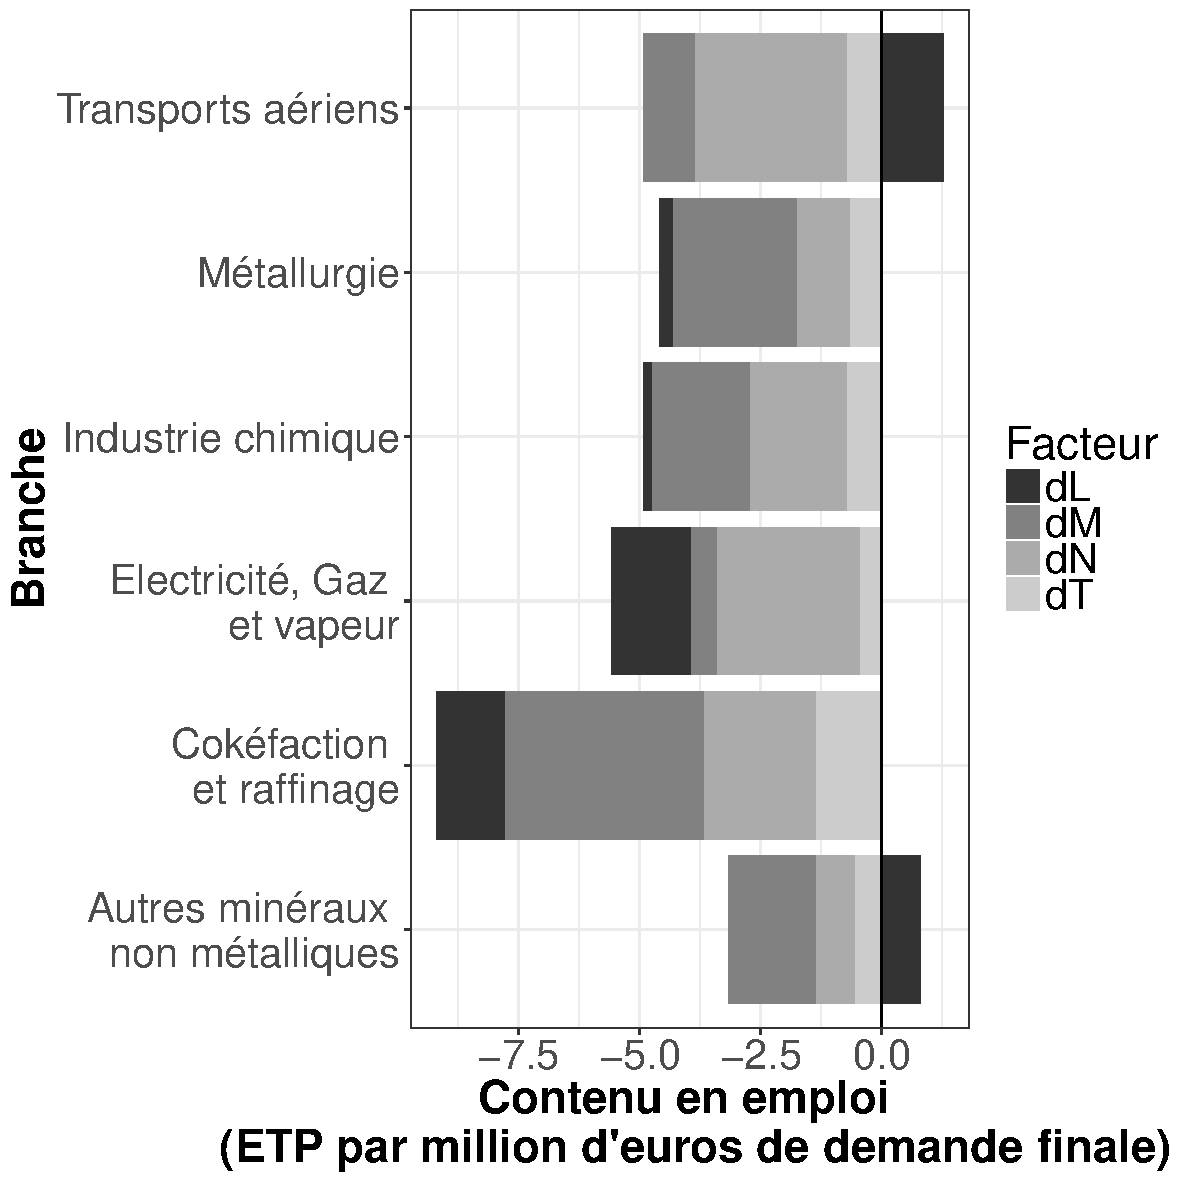
\includegraphics[height=11cm]{figures/GES_et_emplois/EU_ETS.pdf}
	\caption{Décomposition du contenu en emploi dans les branches soumises à l'EU ETS \\
		Sources : Calcul des auteurs à partir de données Eurostat.}
	\label{fig:EU ETS}
	\captionsetup{justification=raggedright}
	\caption*{Lecture : Ce graphique indique la différence entre le contenu en emploi de chaque branche et la moyenne nationale. Nous avons ici agrégé les importations finales et intermédiares : $dM = dMF + dMI$ pour plus de lisibilité. $dL$ indique la part du travail dans la valeur ajoutée, $dN$ le niveau des salaires et $dT$ le niveau de taxes et subventions. On voit que les branches soumises à l'EU ETS ont un contenu en emploi inférieur à la moyenne, principalement du fait d'importations élevées et/ou d'une faible part des salaires dans la valeur ajoutée.}
\end{figure}


\end{subappendices}

\newrefsection
\selectlanguage{english}
\chapter{How shifting investment impacts employment: three determinants under scrutiny} \label{chap:mechanisms}

\section{Introduction} \label{Introduction}

Is it possible to reduce greenhouse gas (GHG) emissions and create jobs at the same time? The double challenge of global warming and unemployment has motivated a long quest for such a panacea. And it remains an acute topic as global warming is likely to exceed 2\degree C by the end of the century and unemployment persists at high post-crisis levels in many countries in Europe and elsewhere.

The urgent need to take action and mitigate global warming is unanimously recognised by the international scientific community. To make substantial and sustained reductions in greenhouse gas emissions, we must transform the way we produce and use energy, through investment in renewable sources of energy, energy efficiency and new infrastructure. The USD 1.8 trillion invested in energy each year \citep{IEAWIR2016} needs to be redirected towards renewable sources. The importance of such a shift was restated in the Paris Agreement: Article 2 recalls the importance of "making finance flows consistent with a pathway towards low greenhouse gas emissions and climate-resilient development". 

Such sums of money have attracted attention with respect to their impacts on the sensitive issue of employment. In various policy communications and media, the potential for so-called “green jobs” is used as a central argument in favour of renewable energy or weatherproofing programs – sometimes even placed above their benefits for the climate. These investments would create jobs because they are more local and labour-intensive than burning fossil fuels in capital-intensive plants. But similar arguments on jobs were also used by Donald Trump to leave the Paris Agreement.\footnote{He insisted on the importance of coal-related jobs in the US. The word "job" was used 18 times in his speech.}

Considering employment impacts as a simple secondary benefit of global warming mitigation would be a mistake. Today, this second dividend is a powerful lever to initiate public action. Although the Paris Agreement has made countries' emissions pledges more ambitious, international negotiations still stumble on a version of the prisoner's dilemma: individually, each nation might try to free-ride as much as possible and let the other countries bear the bulk of the climate burden. This partly explains why the sum of INDC from the Paris Agreement is far from meeting its overall target of staying "well below 2\degree C"\footnote{According to the \citet{OECD/IEA2016}'s World Energy Outlook, the Paris Agreement pledges are "not nearly enough to limit warming to less than 2\degree C"}, while at the same time the IPCC chair, Dr Pachauri, considers that “the solutions are many and allow for continued economic and human development. All we need is the will to change”\footnote{Declaration at the release of the Fifth Assessment Synthesis Report of the IPCC, November 2, 2014}.
As long as ecology and economy are conceived in terms of trade-offs, such difficulties are doomed to continue. The issue of employment is a local matter which can accelerate, as well as hinder, the energy transition transformation. 

But is it possible to generate net positive job creation by simply shifting demand towards environmentally-friendly sectors? 
The literature on this dual topic of environment and economy is known as the "double dividend" debate. It studies under what conditions protection of the environment (the first dividend) can be obtained in conjunction with an economic benefit (the second dividend).
Results from this literature are still mixed, and it is difficult to find robust conclusions. Two main reasons explain this difficulty. The first one is the multiplicity of situations studied: analyses refer to different countries, with various scenarios and data hypotheses on technology costs or production structures. The second reason relates to the variety of tools employed: different economic models are used. In particular, two main families of economic models coexist in the energy-employment literature: Input-Output (IO) models and Computable General Equilibrium (CGE) models. Moreover, it is difficult to disentangle which results stem from the model and which do not. Yet, these two types of model continue to be used in academic publications and reports to policy makers - without comparison between the two.

Our aim is thus to understand the economic mechanisms of job creation due to investment shifts. Why would divesting ourselves of fossil fuels and favouring sectors that will encourage a low-carbon future, such as renewable energy or building insulation, create jobs? Do the arguments about local jobs, domestic sources of energy and labour-intensive technologies hold in a general equilibrium?
Our analysis should also enable us to determine robust results across both types of model, IO and CGE, and to highlight their differences. Do these two types of model yield approximately similar, very different, or even completely opposite results? Answering these questions is necessary in order to test the validity of that part of the literature on green jobs that uses IO models.

Our work is related to the this literature, for which there are many quantitative estimates, using both CGE models \citep{Lehr2008, Lehr2012, Bohringer2013, Blazejczak2014, Creutzig2014, Duscha2014, Duscha2016, Chen2016} and IO models \citep{Hillebrand2006, Scott2008, deArce2012, Markaki2013, Hartwig2016, Yushchenko2016, Li2016, Garrett2017}.
We also use the methodology that \citet{Garrett2017} recently formalised and coined as the "synthetic industry approach" to estimate investment requirements for low-carbon sectors. This new approach helps circumvent the issue of data availability with respect to renewable energies, which was highlighted by \citet{Cameron2015}.
Finally, we also connect to the small strand of literature comparing IO and CGE models, although this work was published outside the energy field. These papers study the employment impacts of an increase in investment, and pointed out that IO models yield higher figures than their CGE counterparts \citep{Partridge1998, OHara2013, Dwyer2005}.

However, our paper has two original aspects. 
First, we go beyond a simple quantification, and disentangle the mechanisms of job creation at play when investment is shifted. 
Our analysis starts with the simpler IO model. We show that, within this framework, the potential for job creation depends on three parameters: the share of labour in value added, the level of sectoral wages and the rates of imports. Shifting investment generates jobs if the shift targets sectors with a higher share of labour in value added, with lower wages or with a lower rate of imports. After a general discussion on these three levers, we test them one by one, using several stylised CGE models, each designed to test a specific assumption.
Breaking down job creation into three levers, and studying each of these levers separately has not yet been done to our knowledge, either for a CGE or an IO model, and even less so for both models together.
Second, we provide quantitative employment estimates of investing in solar PV and weatherproofing, using both an IO model and a fully-fledged CGE. Our two models are based on exactly the same data, at a disaggregated level (58 sectors), with the most recent values available for national accounts (2013). To our knowledge, such a comparison exercise has not yet been undertaken in the energy field. Moreover, our results might differ from the few papers doing the same kind of quantitative comparison in other fields, as the local and labour-intensive characteristics of renewable energies are often quoted as being key to their positive employment potential.

Our analysis indicates that it is possible to generate employment in a CGE by shifting demand towards sectors with a high labour share or low wages. On the contrary, we see no positive impact of targeting sectors with low import rates in a CGE, conversely to many political messages.
IO models provide a good approximation of the impacts of sectoral wage differences on employment. They also provide the right direction for the labour-intensity effect, although overestimating it. But they diverge significantly as to the impacts of trade: IO models demonstrate a strong positive impact of targeting sectors with lower import rates, contrary to CGE models.
Although the literature estimates that employment impacts will always be stronger in IO than in CGE due to the absence of feedback in the former, we show that the price of capital can lead to weaker effects in IO. Considering the source of the employment effect is thus decisive to undertanding the employment impacts and divergences between the two models.
>From a more quantitative viewpoint, investing in solar panels or weatherproofing generates employment in both models. The results are quite similar across models for solar panels. They are higher with IO for weatherproofing, but by a factor from 1.19 to 1.87, a discrepancy much lower than other estimates in the literature. 

The remainder of this paper is organised as follows.
We start with a review of literature in section \ref{sec:literature}. In section \ref{sec:intuition}, we consider a simple IO model, in order to highlight that three mechanisms determine the impact of policy on jobs in IO analysis: the share of labour in value added, wages and rates of imports. We comment on the economic intuitions behind these three potential levers for job creation.
Then, in section  \ref{sec:smallModels}, we discuss the impact of each of these three mechanisms with stylised CGE models.
We go on to give more quantitative estimates in section \ref{sec:fullModel}, using a fully-fledged CGE with 58 sectors and comparing it with IO results.
Finally, section \ref{sec:conclusion} concludes and discusses implications for policy and future research.


%%%%%%

\section{Literature} \label{sec:literature}

Economists have favoured the use of taxes to correct externalities since the work of \citet{Pigou1920}.
But the search for a double dividend (term coined by \citet{Pearce1991}) started with the idea of a carbon tax to mitigate climate change.The initial idea was to tax the negative externalities, i.e. carbon emissions, and use the revenues to reduce more distortionary taxes, thus improving the overall economic performance and reducing pollution at the same time. If the positive impacts ("the revenue-recycling effect") could outweigh the negative impacts ("the tax-interaction effects"), then a "strong" double dividend could be obtained, sensu \citet{Goulder1994}.
The appeal of such a no-regret policy has motivated numerous pieces of theoretical and empirical research. 
In a seminal paper, \citet{Bovenberg1994a} argued that, in a first-best setting, environmental taxes exacerbate distortions in the labour market and in the commodity market, leading to a decrease in employment.
Two years later, \citet{Bovenberg1996} studied the case with unemployment through a fixed wage, and with an unspecified fixed factor. They concluded that a tax on pollution can boost employment if labour is a better substitute for the polluting input than capital. 
An early review of the numerous works on the double dividend was made by \citet{Goulder1994}. \citet{Chiroleu-Assouline2001} provides a summary of theoretical work, and \citet{Patuelli2005} offer a more recent review of 61 quantitative studies on this topic.

This literature has evolved with increasing concerns about global warming and rising unemployment. The employment dividend has become more important. An abundant stream of research has studied whether the energy transition can kill two birds with one stone, through the potential for so-called "green jobs".
Another shift has been the increased perception of inter-sectoral impacts.
In the earlier works, the analytical papers \citep{Bovenberg1994, Bovenberg1996} tried to determine under what conditions a better use of green taxes could reduce unemployment, but they considered an economy with one single sector.
However, the need to invest in new, low-carbon infrastructure has motivated research based on the impacts of investment between different sectors. For example, would it be better to invest in retrofitting buildings or in additional energy sources? in domestically-produced wind turbines, or in cheaper gas-fuelled power plants burning imported gas? 
Models with several sectors became dominant in studying the differences between cost structures and import rates.

In this literature on the energy transition and employment, it is possible to distinguish two broad categories of model that have been used to quantify employment impacts: input-output (IO) models and computable general equilibrium (CGE) models.
Work on input-output models includes \citet{Hillebrand2006, Scott2008, deArce2012, Markaki2013, Hartwig2016, Yushchenko2016, Li2016, Garrett2017}.
Among the most prominent work on CGE models is \citet{Lehr2008, Lehr2012, Bohringer2013, Blazejczak2014, Creutzig2014, Duscha2014, Duscha2016}.

IO models can be considered as a corner-case of CGE, i.e. a CGE model with very specific assumptions. But these assumptions are so specific that IO and CGE can also be considered as different model types. IO's best-known assumptions are Leontief production functions and fixed prices \citep{Miller2009}. \citet{Dwyer2005} list five assumptions underpinning IO models: final demand is exogenous; capital, labour and land are endogenous; there are no price-induced substitution effects; government expenditure remains constant; employment is perfectly elastic. 
Another assumption depends on the category of IO model considered. It is important to distinguish two types of IO model: open (or type I) models and closed (or type II) models \citep{Miller2009}. The differences between these two types lies in the treatment of wages and household consumption. These are endogenized in type II models: additional labour revenues lead to increased consumption, in a circular manner. In this paper, we focus on open models, as they seem more common in the literature. Thus, the remainder of this paper implicitly refers to open models. In this framework, household consumption is exogenous. It is not influenced by labour revenues. 
With all these assumptions, IO models can also be considered as a significant departure from CGE models: by fixing prices, they deviate from the profit-maximising behaviour of the firm in CGEs. By setting exogenous demand, they also differ from the utility-maximising consumer found in CGE models. A possible pitfall of using exogenous investment and fixed prices is the possibility of increasing investment in order to generate employment, without considering how this increase will be financed or the negative impacts on employment at payback time. For example, \citet{Wei2010} estimates the number of jobs per unit of energy produced, thus creating a bias favouring the costlier sources of energy.

Despite these restrictive assumptions, the use of IO models is motivated by a number of comparative advantages over CGEs. The first is their simplicity: IO models are easy and quick to set up. They are easier to combine with technical bottom-up models, for example in the building sector \citep{Scott2008, Yushchenko2016}. Because they are easier to understand, they also avoid the pitfall of being considered as a "black box" which is sometimes the case with large computational models \citep{Faehn2015}.

All these assumptions used in IO models raise the crucial question of the validity of their results. Are IO analyses a good approximation of general equilibrium studies? And if not, what assumptions should be changed?

As an analysis of employment related to the energy transition, our work extends the previous analyses which used only one methodology. In particular, we use the same renewable investment vectors as \citet{Garrett2017}, but add the results from CGE modelling, as well as an explanation of the input-output mechanisms of job creation.

As a comparative exercise, we contribute to the small literature on differences between IO and CGE. 
Other papers that have already mentioned the difference in employment impacts found in IO and CGE models are \citet{Partridge1998, OHara2013}. 
\citet{Dwyer2005} offer a discussion and quantitative comparison of IO and CGE models, at the regional and national level, of the impacts of a special event, an Australian Grand Prix. They find that the employment multiplier is 4.64 higher in the IO model. They point out that there is a crowding out in CGE and not in IO, which to a large extent explains these discrepancies. Other quantitative analyses have studied local or regional impacts \citep{Siegfried2000}, but this is not our focus here. 

Our paper is close to these comparative works, and in particular to the analysis made by \citet{Dwyer2005}, but differs on several points. 
The main one is that we go deeper into the discussion of differences between IO and CGE models. 
We first break down the mechanisms of job creation through a shift in final demand in IO models, and show that they boil down to three components: the relative share of labour in value added, wages, and import rates of the sectors affected by the shift. 
Then, we compare each of these mechanisms with a stylised CGE model. 
In this comparison exercise, we show the corresponding equations of IO and CGE models side by side, and discuss each in turn. Finally, we make a quantitative comparison with a full-fledged CGE, and add a discussion about labour market representation, as well as about the trade-related closure.

The topic under scrutiny is also different. Our focus is the energy transition, not a special event such as a Grand Prix or a stadium investment. We use data for investment in low-carbon sectors. These different data might yield new results, since the high labour content of renewable energy and building insulation is often presented as a lever for job creation. Moreover, it provides comparison between CGE and IO models, which are both used in the literature on the employment effects of an energy transition.

Finally, from a methodological point of view, we do not study an increase in investment, but a shift, a reallocation of the same amount of aggregate investment to different sectors. This approach should alleviate the absence of crowding out effects in IO models, and might provide different results. In addition, this question is of interest for policy makers, as it tries to determine whether job creation is possible with a constrained budget.


\section{Intuitions and assumptions of IO models} \label{sec:intuition}

\subsection{Presentation of input-output models}
Let us first consider IO analyses. What drives employment creation in these models? What are the mechanisms at play?
In input-output, the link between the vector of final demand $\pmb{d}$ and the vector of production $\pmb{p}$ is made by the balance between supply and use at the domestic level \eqref{domestic_balance}, and for imports \eqref{imports_balance}:

\begin{equation}
\pmb{p^d} = \pmb{Z^d} \cdot \pmb{i} + \pmb{d^d}	
\label{domestic_balance}
\end{equation}
\begin{equation}
\pmb{m} = \pmb{Z^m} \cdot \pmb{i} + \pmb{d^m}	
\label{imports_balance}
\end{equation}
where the exponent \textit{\textbf{d}} refers to a domestic item and the exponent \textit{\textbf{m}} to an imported item. 
$\pmb{p^d}$ is domestic production, $\pmb{Z^d}$ et $\pmb{Z^m}$ are the matrices of intermediate consumption, $\pmb{d^d}$ and $\pmb{d^m}$ are the vectors of final demand, and $\pmb{m}$ is the vector of imports. 
$\pmb{i}$ is a vector made of 1. 
Bold and small letters represent a column vector, bold and capital letters a squared matrix. Finally, the exponent \textit{\textbf{t}} represent the sum of imported and domestic items (not to be confused with the transposition operator \textit{t}, not in bold). Thus, total final demand is equal to $\pmb{d^t=d^d+d^m}$, and total intermediate consumption is $\pmb{Z^t=Z^d+Z^m}$.

Equation \ref{domestic_balance} provides a link between domestic demand and output, through a matrix inversion from \ref{domestic_balance}:

\begin{align*}
	\pmb{p^d} &= (\pmb{I} - \pmb{A^d})^{-1} \cdot \pmb{d^d}	
\end{align*}
where $\pmb{I}$ is the identity matrix and $\pmb{A}= (a_{ij})$ is the matrix of technical coefficients defined by $\pmb{Z} = \pmb{A} \cdot \pmb{p}$.

We define the rate of imports in final demand as $\pmb{\tau^m} = 1- \frac{\pmb{d^d}}{\pmb{d^t}}$, and we introduce the hat operator: $\widehat{  }$, which transform a vector $\pmb{x}$ into a diagonal squared matrix $\pmb{\hat{x}}$, so that:
\begin{align*}
	\widehat{x_{ii}} &=x_i \\
	\widehat{x_{ij}} &=0 \quad \forall i \ne j
\end{align*}

then we can further link total final demand to output:
\begin{align*}	
	\pmb{p^d} &= (\pmb{I} - \pmb{A^d})^{-1} \cdot (\pmb{I} - \pmb{\widehat{\tau^m}}) \cdot \pmb{d^t}	
\end{align*}

Finally, employment is linked to production in a linear way, by multiplying production by its average number of jobs. We define the column vector $\pmb{\tilde{e}} = \pmb{fte}/\pmb{p}$, where $\pmb{fte}$ is the vector providing the number of direct full-time equivalent jobs in each sector, at the year of calibration (the reason for the tilde on $\pmb{\tilde{e}}$ will become clear later). 
Then, as we are interested in changes in final demand, we introduce the change operator $\Delta$. 
The relation between variations of final demand and variations of the total number of jobs $FTE$ is:

\begin{align}	
	\Delta FTE &=  \pmb{\tilde{e}}^t \cdot (\pmb{I} - \pmb{A^d})^{-1} \cdot (\pmb{I} - \pmb{\widehat{\tau^m}})\cdot \Delta \pmb{d^t}
	\label{eq:starting_equation}
\end{align}
where $\pmb{\tilde{e}}^t$ is the transpose of the vector $\tilde{e}$. Equation \ref{eq:starting_equation} is the fundamental relation of IO analysis to study employment effects. 

But let us add a small twist in order to make this expression more intuitive. 
Since the entire system of equations is linear, we can link final demand not only to production, but also to value added.
Value added $\pmb{va}$ is equal to the difference between production $\pmb{p}$ and intermediate consumptions $\pmb{Z}$. 
In an index format:
$$va_j = p_j - \sum_i Z_{i,j} =  (1 - \sum_i a_{i,j}) \cdot p_j$$
which translates into a matrix format to:
$$\pmb{va} = (\pmb{I} - \widehat{\pmb{i^t A^d}}) \cdot \pmb{p}$$

By definition, we have the equality: 
$\pmb{\tilde{e}}^t$ = $\pmb{e}^t \cdot (\pmb{I} - \widehat{\pmb{i^t A^d}}) $, where $\pmb{e}$ is the number of jobs per unit of value added, which we label direct employment intensity, or job intensity. The former equation \eqref{eq:starting_equation} can then be written as:
\begin{align}	
	\Delta FTE &=  \pmb{e}^t \cdot \pmb{Q^d} \cdot (\pmb{I} - \widehat{\pmb{\tau^m}}) \cdot \Delta \pmb{d^t}
	\label{eq:starting_equation2}
\end{align}
where  $\pmb{Q^d} = (\pmb{I} - \widehat{\pmb{i^t A^d}}) \cdot (\pmb{I} - \pmb{A^d})^{-1}$. The matrix $\pmb{Q^d}$ is an allocation matrix. It indicates in which sector the value added to respond to final demand is generated. Remember here that domestic demand is equal to domestic value added, so $\pmb{Q^d}$ just allocates final demand, it does not increase value added. This allocation purpose is illustrated by the fact that the sum of each column of $\pmb{Q^d}$ is equal to one.

This new form illustrates the functioning of input-output models. Reading equation \ref{eq:starting_equation2} from the right to the left, it shows that a change in final demand leads to a change in domestic demand (net of imports). This domestic demand is allocated to various sectors by the $\pmb{Q^d}$ matrix, and generates value added. Finally, this value added creates jobs, depending on the job intensity $\pmb{e}$ of each sector. 

\subsection{A simple two-sector economy}
With such a framework, is it possible to create jobs by shifting demand? 
To get a clearer view, we start with a simple example. Let us assume that there are only two goods: 1 and 2, and two production factors: capital and labour. 
A general formulation of the domestic IO balance is given in table \ref{tab:2x2_IO_table}.

\begin{table}
	\centering
	\caption{Domestic IO table for a two-sectors economy}
	\label{tab:2x2_IO_table}
	\begin{tabular}{llllll}
		\toprule
		&  & Activity &  & Domestic Demand & Total \\
		\midrule
		&  & Industries & Services &  &  \\
		Activity & Industries & $Z_{11}$ & $Z_{12}$ & $D_1$ & $P_1$ \\
		& Services & $Z_{21}$ & $Z_{22}$ & $D_2$ & $P_2$ \\
		Value added & Capital income & $K_1$ & $K_2$ &  &  \\
		& Labour income & $L_1$ & $L_2$ &  &  \\
		Total &  & $P_1$ & $P_2$ &  &  \\
		\bottomrule 
	\end{tabular}
\end{table}

In this case, we have the following general formulation for each vector:
$$ \pmb{e} =
\begin{pmatrix} 
e_1 \\
e_2
\end{pmatrix}
$$

$$ \pmb{Q} =
\begin{pmatrix} 
1-\theta_1 & \theta_2\\
\theta_1 & 1-\theta_2
\end{pmatrix}
$$

$$ \pmb{I} - \pmb{\widehat{\tau^m}} =
\begin{pmatrix} 
1-\tau^m_1 & 0\\
0 & 1-\tau^m_2
\end{pmatrix}
$$
The demonstration and full expression of $\theta_1$ and $\theta_2$ are in appendix \ref{app:input_ouput}. 

With such a framework, we can apply equation \ref{eq:starting_equation2} to show that a shift in final demand from sector S1 towards sector S2 generates jobs if and only if:
\begin{equation}
\label{eq:result1}
(1-\tau^m_2) \cdot \left[(1-\theta_2)e_2 + \theta_2 e_1 \right]> (1-\tau^m_1) \cdot \left[ (1-\theta_1)e_1 + \theta_1 e_2 \right]
\end{equation}
The terms between the brackets represent the domestic employment content  $ce^d$, defined as the number of jobs per unit of domestic demand, by 
$$\forall i, \quad ce^d_i = \sum_i e_i \cdot Q^d_{ij}$$
where the $Q^d_{ij}$ act as an allocation key, since $\sum_i Q^d_{ij}= 1$.
The domestic employment content of a sector is high if addressing demand to this sector generates value added in sectors with a high number of jobs per unit of value added.

Equation \ref{eq:result1} reveals that, in input-output analysis, a shift in final demand can create jobs if:
\begin{itemize}
	\item the shift targets sectors with lower import rates $\tau^m_i$
	\item the resulting domestic demand generates value added in sectors with a higher number of jobs per unit of value added $ce^d_i$. 
\end{itemize}	

To make our case clearer, let us consider the simpler case where there is no intermediate consumption. The allocation matrix $\pmb{Q^d}$ becomes the identity matrix, which means all the non-diagonal terms $\theta_i$ become null. And equation \ref{eq:result1} becomes:
\begin{equation}
(1-\tau^m_2) \cdot e_2 > (1-\tau^m_1) \cdot e_1
\label{eq:result1_simplified}
\end{equation}
This last equation indicates clearly that job creation through reallocation of final demand is possible, and depends on two conditions: the import rate $\tau$ and the employment intensity $e$. 

These two levers of action are at the heart of input-output results. And indeed, they rest on what seems to be strong economic intuitions. 
The first intuition is that allocating demand to sectors with lower import rates would result in "in-shoring" jobs by favouring the domestic production system. If imports are seen as losses or leaks of value added, generating jobs in foreign countries, then favouring local sectors helps reduce this leak and increases employment in the country.
The second intuition is to target sectors with high employment content, so as to increase demand for labour. This intuition overlaps with the ideas of labour-capital substitution and job sharing. For example, if one sector is more capital-intensive and another one is more labour-intensive, reallocating demand from the first to the second sector would substitute labour to capital. And if wages are very high in one sector, then concentrating demand on sectors with lower wages could create more jobs with the same amount of value added.

\subsection{Discussing the two intuitions of IO models}

However, the two intuitions that reducing import and encouraging employment-intensive sectors can create jobs are more ambiguous than what they seem at first sight.

\subsubsection{High job intensity or low labour productivity?}

Let us consider first the intuition that favouring labour-intensive sectors would increase employment.
One can note that labour-intensity $e$ is the inverse of labour productivity $\rho$. 
So encouraging sectors with high labour intensity is strictly equivalent to favouring sectors with low productivity. 
Put this way, the conclusion is much less appealing. As Paul \citet{Krugman1997} wrote: “Productivity isn't everything, but in the long run it is almost everything.”. The key idea is that productivity is what defines the real wage in the long term. 
Put this way, favouring low productivity sectors is rather counter-intuitive and can be seen, literally, as counter-productive.

It is possible to further disaggregate the labour-intensity term $e$ in equation \ref{eq:result1_simplified}, in order to better reflect the mechanisms in input-output models. 
This labour intensity is, in our definition, a ratio equal to the number of jobs (in full-time equivalent, or FTE) per unit of value added: $e_i = FTE_i/VA_i$. 
But this direct link between value added and employment hides one important step. In input-output table, value added in each sector is divided between labour compensation and gross operating surplus. Only the labour compensation then leads to direct employment in that sector.
This means that the job intensity in input-output analysis actually depends on two parameters: the share of labour in value added, and the number of jobs per unit of labour compensation. Or, to put it more clearly, the job intensity is the ratio of two values: the share of labour in value added $\tau^L$ and the average wage $w$ in each sector.
Mathematically, we show this by introducing labour compensation $L_i$ in our definition of labour intensity, to make these two new ratios appear:
\begin{equation}
e = \frac{FTE_i}{VA_i} = \frac{FTE_i}{L_i} \cdot \frac{L_i}{VA_i} = \frac{\tau^L_i}{w_i}
\label{eq:job_intensity_decomp}
\end{equation}

This formulation provides a direct interpretation: job-intensive sectors are the ones with a high share of labour in value added and a low wage.
Targeting sectors with a high share of labour might increase employment demand, at least in the short term. 
And encouraging sectors with lower wages seems like a way to share employment: more people get a job out of the same amount of labour remuneration.

\subsubsection{Reduce imports: an all-win?}

The second intuition of IO analysis is that reducing imports would relocate jobs inside the domestic production system. 
This is a mercantilist assumption, a dual view of trade in which exports are good (they increase final demand and thus create jobs) while imports is a leak of value added which generates jobs in foreign countries.
However, such a binary view suffers from two shortcomings. 

First, the view that imports are a loss is a strong assumption with regards to trade theory. "If there were an Economist's Creed, it would surely contain the affirmations 'I understand the Principle of Comparative Advantage' and 'I advocate free trade'. For one hundred seventy years, the appreciation that international trade benefits a country whether it is fair or not has been one of the touchstones of professionalism in economics" wrote \citet{Krugman1987}.
The question whether free trade is the best option has been an ongoing debate for more than thirty years \citep{Krugman1987}. But the arguments against free trade are mostly based on increasing return, imperfect competition and distributional impacts, which are not explicitly modelled in input-output analysis. 
Because of its modelling, IO analyses directly support the idea of a trade policy aiming at reducing imports, rather than a free-trade approach. However, the very crude representation of trade in IO raises a doubt as to the validity of a such a strong result.

Second, input-output analyses based on reducing imports act as if the budget constraint of trade balance does not hold.
The intuitive criticism is that trade balance has to get balanced \textit{eventually}. A country cannot run a trade deficit (or surplus) indefinitely, and a balancing feedback occurs, often through an evolution of the exchange rate: this is the external devaluation. 
Trying to improve the trade balance will only generate short-term benefits, which will vanish as soon as the exchange rate adapts.

However, it is important to specify what is the time horizon of this "eventually". 
The continuous trade deficit of the United States is a counter-example of this budget rule. Other, and more common counter-examples include the regimes of fixed exchanges rates, or common currency.
In particular, in the Eurozone, the trade deficit of one country hardly impacts the exchange rate of the euro, since most European nations trade with each other, and most countries represent a small part of total imports and exports. Inflation discrepancies can then lead to losses in competitiveness and external deficit in peripheral countries \citep{Coudert2013}. In a common currency, restoring trade balance can occur through internal devaluation, rather than external devaluation. But the internal option is much slower, taking years and even decades to adjust wages downwards. 
Within this context of "unbearable slowness of internal devaluation" \citep{Krugman2012}, a hypothesis of fixed unbalanced trade might be a better mid-term approximation than a fixed budget constraint.

Second, it is important to remind that it is possible to suppose that the trade balance constraint is met in input-output analysis. 
Strictly speaking, the assumption of fixed coefficients only applies to the production function. 
As to the evolution of imports and exports, other options  than keeping coefficients fixed are available \citep{Stoleru1969}[p.263]. 
For example, one way to do it would be to assume that the exports are fixed, the total of imports is constant, and the share of imports in each sector is proportional to demand.
But these alternative options are seldom used in practice, at best,  by the input-output community.


\subsection{Three determinants}

Combining equations \ref{eq:result1_simplified} and \ref{eq:job_intensity_decomp}, we get that a shift in demand from sector S1 towards sector S2 increase employment in an input-output model if and only if:
\begin{equation}
(1-\tau^m_2) \cdot \frac{\tau^L_2}{w_2} > (1-\tau^m_1) \cdot \frac{\tau^L_1}{w_1}
\label{eq:result2_simplified}
\end{equation}

In equation \ref{eq:result2_simplified}, we have identified the three determinants of job creation in input-output models for a reallocation of final demand: the rate of imports, the share of labour vs capital in value added, and the wage. 

Such a simple equation has been obtained by assuming that there was no inter-industrial exchange. In practice, an IO model with more than two sectors and with inter-industrial exchanges would yield a more complicated formulation because of the Leontief inverse matrix (which allocates to many sectors the final demand addressed to one sector).
But fundamentally, the underlying logic remains the same. Imports, labour share and wages are the three key parameters.

Such a simple conclusion was also made possible thanks to the simplifying assumptions of fixed coefficients and fixed prices input-output model.
But to what extend would these intuitions and results hold with less constraining assumption, in a general equilibrium framework?
Answering this question would provide a bridge between the two communities of CGE and IO modellers who study job creation linked to the energy transition.

The remainder of this paper is organised as follow.
In the next section, we study separately each of these three determinants, comparing IO and CGE approaches with three toy-models designed for each question. 
Then, in the following section, we compare a full CGE model with 58 sectors to its equivalent IO model, to get quantitative results.


%%%%

\section{Three small scale models} \label{sec:smallModels}
Is it possible to create jobs by simply shifting demand towards more job-intensive sectors? We saw in section \ref{sec:intuition} that the answer was positive with input-output modelling. 
Job creation was made possible through three channels: a higher share of labour in value added, lower wages, and a lower share of imports. 

But do these results stand in a general equilibrium? In this section, we investigate each of these three elements with simple models.

\subsection{The share of labour in value added} \label{subsec:labourShare}
We first test the intuition of input-output related to the labour-intensity in value added. Does encouraging sectors with high labour intensity create jobs? 
To that end, we compare a CGE model with an input-output model.
For the CGE, we consider a simple static model of a closed economy. 
As an input-output model can be considered a special case of a CGE, we can put side by side the corresponding equations of each model. This is done in table \ref{tab:closedModel}. Table \ref{tab:closedModel} highlights that the differences between the two models are:
\begin{itemize}
	\item The production functions and corresponding factor demand functions (eq. 1 \& 2). The IO model uses a Leontief production function, which implies that there is no substitutability between capital and labour. CGE models use a more general constant elasticity of substitution (CES) function with positive levels of elasticity between labour and capital. After conducting a survey of climate-energy models, \citet{VanderWerf2008} noted that "many models use the knife-edge case of a unit elasticity", i.e. a Cobb-Douglas function. However, his empirical estimates led him to "reject	that elasticities are equal to ones", with values at the country level ranging from 0.22 to 0.61. These finding are in line with the literature on capital-labour production functions (see \citet{Antras2004} for a review). Therefore, we should consider and compare in our analysis both Cobb-Douglas functions, as they are widely used, and CES with a lower elasticity of substitution between capital and labour, since they are more empirically founded.
	\item Endogenous vs exogenous household demand function (eq. 4). In the CGE, assuming Cobb-Douglas preferences, the consumption of each good, in volume, depends on the income net of savings, on household preferences and on the price of each good. By contrast, this consumption is entirely exogenous in an IO model. 
	\item Labour supply (eq. 5). In an IO model, wages are fixed, so that there is an implicit assumption of infinitely elastic supply of labour. In a CGE model, it is possible to model other labour market mechanisms. In our analysis, we use the formulation of a wage curve, i.e. a relationship between the price of labour and the unemployment rate, as first evidenced by \citet{Blanchflower1995}. This "empirical law of economics" is now supported by a large number of studies based on microeconomic data \citep{Blanchflower2005}. With a wage curve, wages decrease as the unemployment rate increases. The intuition behind this mathematical formulation can be, for example, a bargaining-power effect: "higher local unemployment makes life tougher for workers [...] and therefore it is not necessary to remunerate those individuals so well" \citep{Blanchflower2005}. 
	\item Capital supply (eq. 7). Capital is also supplied infinitely at a fixed price in IO, which means there is an infinitely elastic supply of capital. On the contrary, in many short-term CGE models, capital is exogenous and fixed in quantity.
\end{itemize}

In input-output, investment is determined exogenously. In order to draw a parallel between IO and CGE, we also model investment in each sector as exogenous in our CGE, in volumes (eq. 8). Savings are then set to be equal to total investment (eq. 9). 
This macroeconomic closure driven by investment implies that savings will be exogenous in volumes as well. But the rate of savings might vary. 
In its discussion of macroeconomic closures, \citet[p. 57]{Sen1963} classified such models with investment-driven closure and unemployment as "general theory models".
Fixing investment exogenously allows to easily represent sectoral reallocation of investments. And it is widely used in the literature \citep{Lehr2008,Lehr2012}.


\begin{table}[!h]
	\centering
	\caption{Comparative equations of IO and CGE models.}
	\label{tab:closedModel}
	\begin{tabular}{llll}
		\toprule
		Num & Description & Standard CGE 1 & IO model \\
		\midrule
		eq1 & Production function& $Z_j=scZ_j \cdot (\sum_h \delta_{h,j} \cdot F_{h,j} ^{\rho^z})^{1/\rho^z}$ &  $Z_j = \min_h(\frac{F_{h,j})}{a_{h,j}})$\\
		eq2 & Factor demand (capital and labour) & $F_{h,j} = ( scZ_j^{\rho^z} \cdot \delta_{h,j} \cdot p^z_j / p^f_h )^{\sigma^z} \cdot Z_j$ & $F_{h,j} = a_{h,j} \cdot Z_j$ \\
		eq3 & Household income & $Inc = \sum_h p^f_h \cdot FF_h$ &  \\
		eq4 & Household demand 	& $C_i = \frac{\alpha_i}{p^c_i} \left(Inc  - S^p\right)$ & $C_i = \overline{C_i}$ \\
		eq5 & Unemployment & $ U =  1 - FF_{LAB}/Pop$ & $p^f_{Lab} = 1$ \\
		eq6 & Labor supply & $log(\frac{p^f_{LAB}}{pc}) = - \gamma \cdot log(\frac{U}{U^0})$ & $p^f_{Lab} = 1$ \\
		eq7 & Capital supply & $FF_{CAP} = \overline{FF_{CAP}} $ & $p^f_{Cap} = 1$ \\
		eq8 & Investment & $I_i=\overline{I_i} $ &  $idem$ \\
		eq9 & Savings & $S^p = \sum_i p^c_i \cdot I_i $ & $idem$ \\
		eq10 & Balance of domestic good & $Z_i = C_i+ I_i$ &  $idem$ \\
		eq11& Balance of factors & $FF_h = \sum_j F_{h,j}$ &  $idem$ \\
		eq12 & Price equality & $p^c_i = p^z_i$ &  $idem$ \\ 
		eq13 & Consumption price index & $p^c=\prod_i \left( p^c_i \right) ^{\alpha_i}$ & $idem$ \\
		\bottomrule
	\end{tabular}
	\caption*{$idem$ indicates that the equation in this row is identical for the two models.
		More information on this model can be found in appendix, section \ref{app:closed_economy}.
		
		When the capital-labour elasticity tends to zero and one, we get the limiting cases of the Leontief and Cobb-Douglas function. In such cases, to avoid issues with zeros, we replace the production function with a zero profit condition for the Leontief case, $p^z_j  = \sum_h p^f_h \cdot a^z_{h,j}$, and for the Cobb-Douglas with the function: $Z_j = b_j \cdot \prod_h F_{h,j}^{\beta_{h,j}}$.
		
		The respective factor demand functions are $F_{h,j}  = a^z_{h,j} \cdot Z_j$ and $F_{h,j}  = \beta_{h,j} \cdot p^z_j \cdot Z_j / p^f_h$.}
\end{table}

Given these differences between CGE and IO, how far are the results from input-output and from our CGE with standard parameter values? 
We apply our model to a simple two-sector, two-good economy, represented by the social accounting matrix (SAM) given in table \ref{tab:SAM_2x2}. 
In this case, we do not consider inter-industry transactions. This helps identify clearly which sector is more job-intensive (normalizing one unit of labour to one job). In this case, it is sector S1, with 9/14=0.64 jobs per unit of value added, against 4/9=0.44 jobs per unit of value added for S2. And studying a case without inter-industry transactions is not a loss of generality, as this matrix of inter-industry transactions is only a reallocation matrix of final demand and value added (cf. section \ref{sec:intuition}).

\begin{table}
	\centering
	\caption{SAM of a two-good, two-sector economy}
	\label{tab:SAM_2x2}
	\begin{tabular}{llllllll}
		\toprule
		& S1 & S2 & LAB & CAP & HOH & INV & Total \\
		\midrule
		S1 &  &  &  &  & 9 & 5 & 14 \\
		S2 &  &  &  &  & 4 & 5 & 9 \\
		LAB & 9 & 4 &  &  &  &  & 13 \\
		CAP & 5 & 5 &  &  &  &  & 1 \\
		HOH &  &  & 13 & 10 &  &  & 23 \\
		INV &  &  &  &  & 10 &  & 10 \\
		Total & 14 & 9 & 13 & 10 & 23 & 10 &  \\
		\bottomrule
	\end{tabular}
	\caption*{LAB: labour compensations; CAP: capital compensations; HOH: households; INV: investment}
\end{table}

Starting from the SAM in table \ref{tab:SAM_2x2}, we compare the impacts shifting of one unit of investment, in volume, from sector S2 towards the more job-intensive sector S1 (using equation 6 in table \ref{tab:SAM_2x2}). 
In a standard IO model, this shift entails an increase in employment of 0.1984.

Our CGE model allows to easily compare the impact of the capital-labour elasticity in the production function, and of the wage curve elasticity.
For the value of elasticity between capital and labour, we consider three cases of a CES production function: a Leontief function, as used in IO models, which implies that capital and labour are perfect complements; a Cobb-Douglas, which is the function used by a majority of climate-energy CGE \citep{VanderWerf2008} and means an elasticity of one; and a CES function with an elasticity of 0.5 as an intermediate value, more in line with empirical estimates \citep{VanderWerf2008, Antras2004}.
For the wage curve, we use a formulation of labour supply as in \citet{Blanchflower2005} (cf. equation 4 in table \ref{tab:closedModel}), and use their value of 0.1 as our central case. But we consider also two other values: $\gamma=0$, to represent fixed wages as in IO models, and $\gamma=0.05$ as an intermediate case.
The employment results of a demand shift in a CGE for all these parameter sets are shown in table \ref{tab:employ_change_closed}. These results highlight the role and importance of labour supply (eq. 4 in table \ref{tab:closedModel}) and the form of the production function. 

We comment this table \ref{tab:employ_change_closed} with five remarks.

First, all the values in the table are positive. This shows that switching final demand towards more job-intensive sectors is a way to generate a positive impact on employment, both in IO and CGE models. The intuition of increasing labour demand by targeting job-intensive sectors holds in a general equilibrium framework. The lower productivity and the wage increase do not cancel out this positive effect.

Second, the impacts on employment are negatively correlated with both the elasticity of substitution between capital and labour, and the elasticity of the wage curve. 
These two results confirm the following intuitions.
If the capital-labour  elasticity of substitution is high, targeting job-intensive sectors will increase demand for labour and its price, but also induce a substitution away from labour and towards. This feedback will lower the increase in labour demand. 
And if the elasticity of the wage curve is high, then the increase in labour demand due to the demand shift will increase wages, which will reduce in turn the demand of labour from firms.  

Third, in the case of fixed real wages (case $\gamma=0$), the impact on employment is identical for the three production functions. And that impact is the highest of all the cases we have considered (0.47). So if one estimates that real wages are constant (for example, in the short term), then the production function has no importance for the labour-intensity impact.

Last but not least, if we compare the results of the CGE with IO, we see that the results of IO are roughly in line with the central case of our CGE analysis. They correspond to a capital-labour elasticity of 0.5 and a wage elasticity between 0.5 and 1. 
Thus, it seems that IO might provide a reasonable approximation to CGE results for the "employment intensity" effect.

\begin{table} [!h]
	\centering
	\caption{Impact of the production function on employment creation, for a shift of one unit of final demand from sector S2 to sector S1}
	\label{tab:employ_change_closed}
	\begin{tabular}{c|ccc}
		\toprule
		Wage curve & \multicolumn{3}{c}{Capital-labour elasticity} \\
		elasticity & Leontief & CES & Cobb-Douglas \\
		($\gamma$)  &($\sigma_{KL}=0$) & ($\sigma_{KL}=0.5$) & ($\sigma_{KL}=1$) \\
		\midrule
		0 			  & 0.47445 & 0.47445 & 0.47445 \\ 
		0.05		& 0.45392 & 0.24181 & 0.17001 \\
		0.1 	 	 & 0.43505 & 0.16736 & 0.10676 \\
		\bottomrule
	\end{tabular}
	\caption*{These results can be compared to the positive impact in a standard IO model: 0,1984 for the same shift in final demand.}
\end{table}

In all these variants, we have considered that the fixed factor, capital in our case, was fixed in quantity.
Let us now add a word on the importance of this assumption. The extreme opposite would be to posit that the price of capital is fixed, and thus that capital supply is potentially infinite (this is similar to setting $\gamma=0$ with labour).
However, in that case of fixed capital price, a shift of final demand does not create jobs in any of the configuration we have studied.
This result reveals that the decrease in capital prices is an essential component of job gains in a CGE.	
This can help explain why the CGE provides higher estimate of job creation than the IO model when the elasticities of the wage curve and labour-capital substitution are low. The CGE then combine a strong increase in labour demand with a decrease in capital prices, while capital price is fixed in a IO model. 
Thus, the purchasing power increases more in a CGE than in IO, triggering a positive feedback on labour supply.

In conclusion of this section, both a CGE and input-output analysis conclude to job creation when there is a shift in investment towards more job-intensive sectors. The amount of jobs created is similar between the two models. 
However, this convergence hides two diverging mechanisms. 
On the one hand, the production function of a CGE allows substitution between capital and labour, contrary to an IO model. Thus, the increased demand of good translates into a relatively lower increase in labour demand in a CGE. 
On the other hand, there is a decrease in capital price in a CGE, which increases the real wage and thus the supply of labour. Conversely, capital price is fixed in IO.
These results extend to several sectors the findings of \citet{Bovenberg1994, Bovenberg1996}, and are in line with the findings of \citet{Quirion2007}.


\subsection{Sectoral wage differences} \label{subsec:wageDifference}
We now investigate the question of sectoral wage differences.
We expand the model of the previous section in order to account for wage differences between sectors. In the previous section, our CGE formulation assumed a unique wage across all sectors, while in this section we consider a specific wage for each sector. Such an assumption of heterogeneous wages is in line with the data observed in national accounts. 

One explanation for the wage difference is the variety of labour skills required in each sector. Some sectors might require more skills, and this higher productivity leads to higher wages in a neoclassical framework. We explore this assumption in section \ref{subsubsec:labourSkills}.

But other reasons might explain these sectoral wage difference. There could be an imperfect mobility of labour between sectors. For example, \citet{Duhautois2005} showed that most labour mobility occurs within the same sector in France. An extreme case is to assume there is no mobility, and a fixed pool of workers in each sector. This could be the case in the short-term, because of inertia in training, imperfect information, etc.
Another reason, although linked to the imperfect mobility, comes from a more institutional view, in which wages are not only affected by productivity, but also by a balance of power in the bargaining between workers, unions and employers. \citet{Askenazy2016} defends this theory. He shows that two sectors can be identical (e.g. the underground in London and in Paris), but the worker in one sector get higher wages because workers are better organized. His work highlights that bargaining can be sector-specific, and disconnected to a certain extent from the Marshallian framework of supply and demand.
We explore the assumption of wages variation for other reasons than skills in section \ref{subusbsec:fixedWages}, through the assumption of sectoral fixed wages.


\subsubsection{Sectoral differences with labour skills} \label{subsubsec:labourSkills}
In this section, we explore the impact of labour skills on wages and employment. We model two levels of qualification in the labour force: low skilled and high skilled. 
They are modelled as imperfect substitutes, and form a labour composite which is then aggregated with capital.
In each sector, these two qualifications are present, but their respective shares vary. 
The supply of workers of each type is modelled with a wage curve.
An overview of this model is given in appendix \ref{app:two_labour_model}.

More specifically, we consider an economy with the SAM shown in table \ref{tab:SAM_twolabours}.
Capital and labour remuneration are identical in the two sectors. 
But we suppose here that there is a higher share of qualified workers in sector S2 than in S1. The number of workers of each type is given in table \ref{tab:labour_type}. 

\begin{table}
	\centering
	\caption{A 2x2 economy with wage differences}
	\label{tab:SAM_twolabours}
	\begin{tabular}{lllllll}
		\toprule
		& S1 & S2 & LAB & CAP & HOH & INV \\
		\midrule
		S1 &  &  &  &  & 9 & 5 \\
		S2 &  &  &  &  & 9 & 5 \\
		LAB & 9 & 9 &  &  &  &  \\
		CAP & 5 & 5 &  &  &  &  \\
		HOH &  &  & 18 & 10 &  &  \\
		INV &  &  &  &  & 10 &  \\
		\bottomrule
	\end{tabular}
	\caption*{And the employment in sector S1 and S2, in volume, are 9 and 4.5 respectively. The wage ratio between the two sectors is thus 2.}
\end{table}

Because of the higher share of skilled workers in S2, there is a higher wage in S2 and less jobs for the same amount of labour compensation.
In our example, the average salary is twice as high in sector S2 as in sector S1. S2 is less job-intensive than S1, with 8 workers against 6 for the same amount of value added and labour compensation.

\begin{table}
	\centering
	\caption{Initial number of workers by type}
	\label{tab:labour_type}
	\begin{tabular}{lllllll}
		\toprule
		& S1 & S2 \\
		\midrule
		Low-skilled & 7 & 3 \\
		High-skilled & 1 & 3 \\
		\bottomrule
	\end{tabular}
	\caption*{With an initial wage of 1 in sector S1 and 2 in sector S2.}
\end{table}

With this setting, reallocating final demand from sector S2 towards the lower-paying job-intensive sector S1 increase employment by 0.143.
Surprisingly, this figure is not sensitive to the wage curve elasticity, nor to the degree of substitutability between the two types of labour. 

With an IO model, the impact of shifting one unit of final demand from S2 to S1 yields a positive employment impact of 0.143. The share of each labour type remains constant, due to the Leontief production function. 

The results are thus similar with our CGE and IO models. The impact of skilled-specific wages is robust across the two models.


\subsubsection{Sector-specific labour with exogenous wages} \label{subusbsec:fixedWages}

Here, we consider a formulation in which labour is sector specific. There is no mobility of labour between sectors, and only one kind of labour in each sector.
To represent sectoral wage differences, we assume this time fixed, exogenous wages in each sector. This is in line with the fixed salaries in IO. This model is a simple representation and an extreme case of our second and third explanations on sectoral wage differences.
We take again the example of a 2x2 economy, as shown by the SAM in table \ref{tab:SAM_twolabours}.
The two sectors present the same amount of capital and labour remuneration. 
However, we suppose that exogenous wages are twice as high in sector S2 as in sector S1 (we normalise these wages to 1 in sector S1 and 2 in sector S2).
Thus, the job intensity in sector S1 is twice as high as in sector S2.
We investigate the impact of this difference in sectoral wages. 

In our CGE with constant wage, a shift in final demand leads to an increase in employment of 0.321. This holds true for every production function. In our simulation, prices and wages remain constant, so all production functions behave like the Leontief one. 

In input-output, a shift in investment from S2 towards S1 yields a positive impact on employment, due to the lower wages in S1. 
Other things being equal, the value added from final demand generates the same amount of labour compensation. These compensations lead to more jobs (but jobs with lower wages).
In our example, a shift of unit of investment from S2 to S1 leads to an increase in employment of 0.321. 
With our CGE model, the same investment shift yields the same employment impact.

This comparison shows that under the assumption of fixed wages, the effects of sector-specific wage differences are similar in CGE and IO models. 

\subsubsection{Conclusions on wage differentials}
We have studied the impact of wage sectoral difference with two simple frameworks. 
The first one focused on the differences in labour skills across sectors. 
The second one considered sector-specific labour with exogenous wage difference between sectors, which can represent bargaining power as well as intersectoral training and reconversion inertia.
In both these frameworks, the results of IO and CGE modelling were identical as to the impact of sectoral wages differences. 


\subsection{The share of imports: favouring local production?} \label{subec:importShare}
We now turn to the part related to imports. How different is the impact of trade between an IO model and a CGE?
To investigate this question, we start again from our first stylised CGE model from subsection \ref{subsec:labourShare}, but this time we add a representation of trade.

We use a modelling framework similar the standard CGE presented in the textbook by \citet{Hosoe2010}. For imports, we consider an imperfect substitution between domestic and imported products through the use of an Armington specification. For exports, we consider a perfect substitution with the domestic good
%. In other words, we model a constant elasticity of transformation (CET) function between exports and domestic goods with an infinite elasticity
(eq. 19-21). 

Finally, we make the assumption of a small economy for both imports and exports. At a given world price, the country can import as much as it wants from the rest of the world, which is an infinite supplier at a fixed price (eq14). And the country can export infinitely to the rest of the world at a given price (eq. 13). These assumptions are in line with the hypothesis of fixed prices in IO models.

A more complete description of this model is available in appendix \ref{app:open_economy_model}.

In table  \ref{tab:openModel}, we list the equations of the open-economy CGE and IO models.
Compared to the closed version, this new table highlights that there are three additional differences between a CGE and an IO model: 
\begin{itemize}
	\item The first one is the assumption about trade closure (eq. 8). IO models consider that foreign savings are endogenous, which means there is infinite supply of foreign savings at given world prices. CGE models present two options for trade closure. This is because moving from a closed to an open economy adds one equation (the trade balance, eq. 15) and two new variables: foreign savings $S^f$ and exchange rate $\epsilon$. One of these two variables has to be defined exogenously to close the model. Choosing $\epsilon$ as exogenous, and keeping it constant is similar to IO models, which assume constant prices so a constant real exchange rate $\epsilon$. This closure also allows to study movement in the trade balance. Choosing $S^f$ is the opposite option. It means the country cannot borrow more from the rest of the world. Any change in investment or revenue has to be financed domestically.
	
	\item The second difference is the Armington function of the CGE and its corresponding demand functions for imports and domestic good (eq. 16-18). 
	The original idea of \citet{Armington1969} was to present a theory of demand that distinguishes products based on their place of production. 
	%But this Armington specification can also be used as a a proxy to represent the fact that one sector of an economic model regroups a variety of different goods, hence imperfect substitutes. This is in line with the findings that "the level of aggregation is important; the more disaggregate the sample the higher the estimated [Armington] substitution elasticity" \citep{McDaniel2002}. 
	With this modelling, the volume of imports depends on the ratio of prices between the Armington composite good and the imported good. On the contrary, volumes of imports are fixed in share in an IO model. 
	%The choice of an Armington specification implies a certain level of monopoly power for the country in the CGE, with terms of trade effects, which are absent from IO models.
	
	\item The third difference relates to exports. IO models assume exogenous, often fixed, volumes of export. In other words, demand from the rest of the world is considered perfectly inelastic. On the contrary, in our CGE model, we assume an infinitely elastic demand from the rest of the world (eq. 13). These are two polar cases for modelling exports. With respect to exports, IO models diverge largely from the literature, which finds that export price elasticities are below one \citep{Ducoudre2014}.
\end{itemize}

\begin{table}[!h]
	\centering
	\caption{Comparative equations of IO and CGE models. Identical equations are not repeated to facilitate reading. The main differences with the closed version shown in table \ref{tab:closedModel} have their equations labelled in bold.}
	\label{tab:openModel}
	\begin{tabular}{llll}
		\toprule
		Num & Description & Standard CGE 2 & IO model \\
		\midrule
		eq1 & Production function & $Z_j=scZ_j \cdot (\sum_h \delta_{h,j} F_{h,j} ^{\rho^z})^{1/\rho^z}$  &  $Z_j = min_h(\frac{F_{h,j})}{a_{h,j}})$\\
		eq2 & Factor demand & $F_{h,j} = ( scZ_j^{\rho^z} \cdot \delta_{h,j} \cdot p^z_j / p^f_h )^{\sigma^z} \cdot Z_j$ & $F_{h,j} = a_{h,j} Z_j$ \\
		eq3 & Household income & $Inc = \sum_h p^f_h \cdot FF_h$ & $idem$ \\
		eq4 & Household demand of goods  & $C_i = \frac{\alpha^U}{p^x_i} \left( Inc - S^p\right)$ & $C_i = \overline{C_i}$ \\
		eq5 & Unemployment & $ U =  1 - FF_{LAB}/Pop$ & $p^f_{Lab} = 1$ \\
		eq6 & Labor supply & $\log(\frac{p^f_{LAB}}{pc}) = - \gamma \log(U/U^0) $ & $p_{Lab} = 1$ \\
		eq7 & Capital supply & $FF_{CAP} = \overline{FF_{CAP}} $ & $p^f_{CAP} = 1$ \\
		eq8 & Investment & $I=\overline{I} $ & $idem$ \\
		eq9 & Private savings & $S^p = \sum_i p^x_i I_i - \epsilon \cdot S^f$ & $idem$ \\
		\textbf{eq10} & \textbf{Trade closure} & $S^f = \overline{S^f}$  \quad OR \quad $\epsilon = \overline{\epsilon}$ & $\epsilon = \overline{\epsilon}$ \\
		eq11 & Balance for domestic good & $Q_i = C_i + I_i$ &  $idem$ \\
		eq12 & Balance for factors & $FF_h = \sum_j F_{h,j}$ &  $idem$ \\
		eq13 & Price equality & $p^x_i = p^z_i$ & $idem$ \\ 
		eq14 & Consumption price index & $p^c=\prod_i \left( p^x_i \right) ^{\alpha^u_i}$ & $idem$ \\
		\textbf{eq15} & \textbf{Export demand} & $p^e_i=\epsilon \cdot \overline{p^{We}_i}$ &  $E_i = \overline{E_i}$ \\
		eq16 & Import supply & $p^m_i=\epsilon \cdot \overline{p^{Wm}_i}$ & $idem$ \\
		eq17 & Trade balance & $\sum_i \overline{p^{We}_i} E_i + S^f = \sum_i \overline{p^{Wm}_i} M_i$ & $idem$ \\
		\textbf{eq18} & \textbf{Armington function} & $Q_i = scQ_i (\alpha^m_i M_i^{\rho_Q} + \alpha^d_i D_i^{\rho_Q}  )^{1/\rho_Q} $ &  $p_i^Q Q_i + p_i^e E_i = p^m_i M_i + p^d_i D_i$ \\
		\textbf{eq19} & \textbf{Imports demand} & $M_i = \left( scQ_i^{\rho_Q} \cdot \alpha_i^m \cdot \frac{p_i^Q}{p_i^m} \right)^{\sigma_Q} Q_i$ & $M_i=\lambda^m_i \cdot (Q_i+E_i)$\\
		\textbf{eq20}  & \textbf{Domestic demand} & $D_i = \left( scQ_i^{\rho_Q} \cdot \alpha_i^d \cdot \frac{p_i^Q}{p_i^d} \right)^{\sigma_Q} Q_i$ & $Z_i=\lambda^z_i \cdot (Q_i+E_i)$\\
		eq21 & CET function & $Z_i = E_i + D_i$ & $idem$ \\
		eq22 & Supply of E & $p_i^e = p_i^z $ & $idem$ \\
		eq23 & Supply of D & $p_i^d = p_i^z  $ & $idem$ \\
		\bottomrule
	\end{tabular}
\end{table}

To estimate the impact of these differences in the modelling of trade, we consider again a two-sector, two-good economy. In this case, we suppose that the two sectors are identical, except for their shares of imports. The corresponding SAM is represented in table \ref{tab:openEconomy}.
Again, we set the matrix of intermediate consumption to zero in order to make our case more intuitive, without loss of generality.

\begin{table}[!h]
	\centering
	\caption{SAM of an open economy}
	\label{tab:openEconomy}
	\begin{tabular}{llllllll}
		\toprule
		& S1 & S2 & LAB & CAP & HOH & INV & EXT \\
		\midrule
		S1 &  &  &  &  & 8 & 4 & 3 \\
		S2 &  &  &  &  & 12 & 4 & 3 \\
		LAB & 9 & 9 &  &  &  &  &  \\
		CAP & 5 & 5 &  &  &  &  &  \\
		HOH &  &  & 18 & 10 &  &  &  \\
		INV &  &  &  &  & 8 &  &  \\
		EXT & 1 & 5 &  &  &  &  &  \\
		\bottomrule
	\end{tabular}
\end{table}

We now simulate a shift of one unit of investment from S2 towards S1, the sector with lower import rates. A quantitative detail of the results is available in appendix \ref{subsec:open_economy_results}, but we highlight here the main idea. 

In IO, there is a positive effect of targeting the sector with lower import rates. The total amount of imports is reduced by 0.2, while exports remain constant by assumption. The net balance of trade improves by 0.2. And these import reductions translate into an increase in domestic production and domestic value added (+0.2), which in turn generate more jobs. Overall, there is an increase in labour by 0.07 in IO.

In our CGE, let us first consider the first trade closure, with endogenous exchange rate $\epsilon$ and constant foreign savings $S^f$. Results are given in table \ref{tab:SAM_CGE_openEconomy}. Within this framework, a reallocation of final demand towards S1 increases imports in S1 (+0.08) and decreases imports in S2 (-0.31), for an overall reduction in imports (-0.23). But this overall decrease in imports is met by an equal reduction in exports (-0.92 in S1 and +0.69 in S2, for a net reduction of 0.23).
Private consumption is left unchanged.
Overall, the shift in demand decreases imports, but it translates into lower exports rather than higher domestic production. This is a clear divergence with IO results. Reallocation of final demand does not create jobs through the import channel in a CGE in a flexible exchange rate regime. They only lead to a shift of the labour force towards S1. 
These results are insensitive to the choice of the Armington elasticity, even if we consider different elasticities for the two sectors. 

\begin{table*}[!h]
	\centering
		\caption{CGE results in an open economy with fixed foreign savings $S^f$}
		\label{tab:SAM_CGE_openEconomy}
		\begin{tabular}{llllll}
			\toprule
			& S1 & S2 & HOH & INV &  EXT\\
			\midrule
			S1 &  &  & 8.00 & 5.00 & 2.08 \\
			S2 &  &  & 12.00 & 3.00 & 3.69 \\
			LAB & 9.00 & 9.00 &  &  &  \\
			CAP & 5.00 & 5.00 &  &  &  \\
			EXT & 1.08 & 4.69 &  &  &  \\
			\bottomrule
		\end{tabular}
\end{table*}
%\vspace{5cm}
\begin{table*}[!h]
		\centering
		\caption{Open economy with fixed exchange rate $\epsilon$ and fixed exports}
		\label{tab:SAM_IO_OpenEconomy_noBudget_fixE}
		\begin{tabular}{llllll}
			\toprule
			& S1 & S2 & HOH & INV & EXT \\
			\midrule
			S1 &  &  & 7.88 & 5.00 & 3.00 \\
			S2 &  &  & 11.82 & 3.00 & 3.00 \\
			LAB & 9.52 & 8.48 &  &  &  \\
			CAP & 5.29 & 4.71 &  &  &  \\
			EXT & 1.07 & 4.63 &  &  &  \\
			\bottomrule
		\end{tabular}
\end{table*}

With these hypotheses, the model is unstable: household consumption increases by almost 40\% and exports drop to zero, as shown in table \ref{tab:SAM_IO_OpenEconomy_noBudget}. Consumption is financed through a raise in foreign investment (+7.41). But this increased consumption is a model artefact, as the model does not account for the payback of this foreign loan. This result highlights that the two assumptions of IO models regarding the behaviour of imports and exports are necessary in order to avoid a strong and artificial change in trade patterns. 

We now look at the alternative trade closure for the CGE, with exogenously fixed exchange rate and endogenous foreign savings. However, if we only change this assumption, household will stop exporting as they do not need to pay for their imports any more (cf. table \ref{tab:SAM_IO_OpenEconomy_noBudget} in appendix). 
To avoid the bias of vanishing exports, we test a second formulation. We keep the constant exchange rate and assume, in addition, that exports are constant, as in IO models. With this formulation, a shift in investment towards sector S1 does improve the trade balance (see table \ref{tab:SAM_IO_OpenEconomy_noBudget_fixE}). 
Imports slightly increase in sector S1, but decrease more in sector S2, leading to an overall reduction of imports. There is also a job shifting towards S1.
However, there is no increase in wage nor any increase in employment. The reduction in imports does not translate into more jobs, but into less private consumption, and thus a lower utility.
In IO models, private consumption was supposed to be constant and exogenous. But in a CGE, if we assume constant exports like in an IO model, a shift entails a decrease in private consumption.

This comparison between an IO model and a CGE model for an open economy yields two conclusions. 
First, the assumptions of fixed exports in an IO model is very strong, considering that exports vary in a CGE model when investment changes. Such a hypothesis of constant exports should be justified. 
Second, a shift towards a sector with lower import can lead to a shift in the labour force, but does not increase employment in a CGE. This holds true for the two possible trade closure: an exogenous exchange rate and exogenous foreign savings.
This conclusion is a strong case against the second intuition of IO analysis: reducing imports is not a lever to create jobs. 

%%%%%%




\section{Full model comparison} \label{sec:fullModel}

In this section, we turn to a more quantitative analysis of the employment impact of CGE and IO models.
The stylized examples of the previous sections have helped identify the three major determinants of employment creation in IO models, and how they change in a CGE model.
We now turn to a comparison of fully-fledged IO and CGE models, with 58 sectors.
This section will thus bring together the previous parts, adding up the effects and identifying the possible interactions. It will provide quantitative results on job creation, while the previous section was more qualitative. 

In addition, a complete model takes into account some aspects that have so far been omitted. In particular, this last CGE model will consider the role of the government and tax collection. This aspect is often neglected in input-output analyses. With IO models, the presence of taxes or subsidies can induce a bias in employment content, artificially raising or reducing it for some sectors \citep{Perrier2017}.
To avoid this bias, the change in government revenues should be corrected in IO analyses. But this aspect is rarely mentioned and even less dealt with.
By contrast, in the CGE, we will consider that the government's budget constraint is met, taking into account all sources of revenue. 
Thus, an increase in investment in sectors with low taxes or high subsidies will lead to an increase in direct taxes on households, so that government revenues remain constant.


\subsection{Scenario}
We focus on two case studies: the improvement of building weatherproofing, and the installation of solar panels on roofs. 
An investment in weatherproofing decreases the need for heating, and thus the consumption of gas or electricity, depending on the heating system. Similarly, an investment in private solar panels will lead to self-sufficiency in power, thus reducing electricity consumption from the network. 
In each case, we suppose that a cost-effective investment exists; in other words, that the discounted benefits of reduced consumption are equal to the initial investment costs. This assumption allows us to focus on the difference in employment impacts, all other things being equal. And this seems plausible in both cases: the rapidly-falling costs of solar panels have made this technology competitive, or close to competitive, in many countries\footnote{According to the \citet{InternationalEnergyAgency2015}, "at the low-end costs [of renewable technologies] are in line with – or even below – baseload technologies".}; refurbishment can also be competitive\footnote{In another report, the \citet{InternationalEnergyAgency2013} states that "Some of the technologies needed to transform the buildings sector are already commercially available and cost effective, with payback periods of less than five years"}.

We also suppose that power and heat production are determined by the technological environment and by the "basic needs" to heat a house and power all white goods. From a modelling perspective, we use a Stone-Geary utility function, with a subsistence consumption level (the basic need) for the electricity, gas and heat sector.
With these hypotheses, the exogenous basic need is formally equivalent to an exogenous investment. The results of the previous sections can thus be applied.

We study a scenario with an investment of one billion euros in weatherproofing or solar panels, and a (discounted) reduction in consumption of one billion in the power, gas and heat sector.
The results are compared to the initial equilibrium. 


\subsection{CGE model description}
Our CGE model is based on a textbook by \citet{Hosoe2010}, the equations of which are available in the GAMS community \footnote{\url{https://www.gams.com/latest/gamslib\_ml/libhtml/gamslib\_stdcge.html}} online model library. 
We use this standard model in order to avoid as far as possible any "black-box" criticism, and to provide general, standard results.

Our CGE model is based on the exact same input-output table used in the IO analysis. But it adds an additional layer with flexible prices and utility maximization of households based on consumption.

Government taxes production, final household consumption and investment at constant rates.  It also directly taxes a fraction of household revenues. Capital supply is fixed. 

This model incorporates the assumption of a small economy, which means that foreign prices are considered fixed. Supply of imports and demand for exports are assumed to be infinitely elastic.
Demand for imports is represented through an Armington specification. Exports and domestic goods are assumed to be imperfectly substitutable, as represented by a CET function.

We make only three changes to \citet{Hosoe2010}'s textbook model, in order to adapt it to our research question. 
First, we expand the modelling of the labour market. We introduce two skill levels for labour: low and high, in order to represent and explain wage differences between sectors. And we replace the assumption of fixed labour by a wage curve, in order to study the impact of investment policies on employment.
Second, we modify the macroeconomic closure. Instead of closure being driven by a fixed saving rate, we use a closure based on exogenous investments (as was the case with our small-scale examples). This new closure allows a better parallel with IO models, in which investments are exogenous; and it is commonly used in the literature on green jobs \citep{Lehr2008,Lehr2012}.
Third, we make government consumption exogenous and constant, in order to avoid variations in government expenditure which may cloud results for employment. The government adjusts its budget by choosing the rate of direct tax on households. It also collects taxes from production and consumption, but at fixed rates.

More information on this model can be found in appendix \ref{sec:full_model}.

\subsubsection{Data}
To calibrate our model, we use four data sources in our analysis. The first three are collected and provided by the French national institute of statistics, the INSEE. The last one is from \citet{Garrett2017}.
\begin{itemize}
	\item The 2013 input-output tables for France, at the 64 product levels, based on the NACE Rev. 2 classification. One table represents the French domestic balance between supply and use, and the other represents the total French economy. The difference between these two tables yields the import table.
	\item The number of full-time equivalent (FTE) jobs, at the same level of disaggregation and with the same classification.
	\item The amount of tax collected by the government. We use the table of integrated economic accounts produced by INSEE.\footnote{\url{https://www.insee.fr/en/statistiques/2561550?sommaire=2387999}}
	\item Finally, the cost structures of solar PV and weatherproofing. We use the literature review provided by \citet{Garrett2017}.
\end{itemize}

However, to avoid issues relating to negative values, we aggregate some sectors (see appendix \ref{app:full_model_data} for more details). With these modifications, we end up with 58 sectors. We apply the same grouping to the employment data.

We estimate the investment vectors in weatherproofing and solar PV from \citet{Pollin2015}. These vectors are shown in table \ref{tab:IO_vectors}.

\begin{table}[!h]
	\centering
	\caption{IO vectors from \citet{Pollin2015} as quoted by \citet{Garrett2017}}
	\label{tab:IO_vectors}
	\begin{tabular}{p{0.4\linewidth}cc}
		\toprule
		Label  & Solar & Weatherproofing \\
		\midrule
		Construction& 0.3 & 1 \\
		Fabricated metal products& 0.175 &  \\
		Machinery& 0.175 &  \\
		Computer and electronic products& 0.175 &   \\
		Miscellaneous professional, scientific, and technical services& 0.175 &   \\
		\bottomrule
	\end{tabular}
\end{table}


\subsubsection{Preliminary analysis of energy sectors}
Before turning to the numerical application, let us examine a few metrics to understand the mechanisms at work, in line with the analysis in section \ref{sec:smallModels}. The import rate, share of labour, wages and employment content of the sectors under consideration are shown in table \ref{tab:descriptiveRatios}. 
For solar and weatherproofing, the ratios are based on the synthetic industry approach of \citet{Garrett2017}: we use a weighted average of existing sectors, using the weights indicated in table \ref{tab:IO_vectors}.
The import rate, wages and employment levels are direct measures for each sector. They represent only the first-round effect, not all the inter-industry effects. But they provide a first-order approximation as to the employment impacts of targeting each sector.
In France, the "electricity and gas" sector has a low share of labour in value added, as well as high salaries, compared to solar panels and weatherproofing. As shown in our previous analyses in section \ref{sec:smallModels}, these two factors will induce job creation when investing in solar or weatherproofing, at the expense of the traditional electricity or gas sector.
The third factor, import rates, is higher for solar panels: 23\% against 0\% for weatherproofing and 0.5\% for electricity and gas. This latter value might seem quite low, but this is partly because fossil fuels only represent 17\% of the French power mix in 2017, due to a high proportion of nuclear energy and hydro-electric power. In a CGE, the high import rate of solar panels should not play a major role (cf. section \ref{subec:importShare}), but it has a negative effect on employment in IO analysis (and conversely a low import rate import has a positive effect on employment in IO).

\begin{table}[!h]
	\centering
	\caption{Descriptive direct ratios}
	\label{tab:descriptiveRatios}
	\begin{tabular}{p{0.2\linewidth}p{0.1\linewidth}p{0.1\linewidth}p{0.1\linewidth}}
		\toprule
		& Import rate (\%) & Share of labour in value added (\%) & Wages (\euro / ETP)  \\
		\midrule
		Solar & 23 & 81 & 56 \\
		Weatherproofing & 0 & 82 & 48 \\
		Electricity, gas and air-conditioning & 0.5 & 39.2 & 92.5 \\
		\bottomrule
	\end{tabular}
\end{table}


\subsection{Results}
We now run the CGE model with central values for all parameters (sensitivity analyses will follow), as well as the IO model. 
For each model, we compute the number of jobs created by investing one billion euros in the technology indicated in the first column (solar panels or weatherproofing), and reducing electricity or gas consumption by the same amount.
We can then calculate the \textit{discrepancy ratio} between the two models, i.e. the number of jobs created in IO divided by the number of jobs created in the CGE.
Table \ref{tab:results} shows that encouraging refurbishment or the installation of solar panels both generate positive employment impacts.
In line with our preliminary analysis, we can link these effects to the higher share of labour in value added, as well as to the lower wages in those sectors, compared to the "electricity and gas" sector.
Second, we measure a discrepancy ratio of 1.07 and 1.51 for solar and weatherproofing respectively. The IO model yields higher estimates, but the discrepancy is smaller than other values in the literature. For example, \citet{Dwyer2005} found a ratio of 4.6 (but for a very different scenario: he was studying the impacts of a Grand Prix).

\begin{table}[!h]
	\centering
	\caption{Employment impacts of investing in solar panels or weatherproofing \\ (in full-time equivalents for an investment of one billion euros)}
	\label{tab:results}
	\begin{tabular}{lccc}
		\toprule
		Techno & Job creation in CGE* & Job creation in IO & Discrepancy ratio \\
		\midrule
		Solar & 4,670 & 5,010 & 1.07 \\
		Weatherproofing & 5,331 & 8,050 & 1.51 \\
		\bottomrule
	\end{tabular}
	\caption*{*For a capital-labour elasticity $\sigma_{KL}$ = 0.5 and a wage curve elasticity $\gamma$ = 0.1}
\end{table}


\subsection{Sensitivity analyses}

\subsubsection{Impact of the wage curve and capital-labour elasticity}
The employment results of a shift in final demand are represented in table \ref{tab:wageCurve} for the CGE model.

For all the values considered, there are positive employment impacts, but both the wage curve elasticity and the capital-labour elasticity have a strong influence on results. The employment impact decreases with both wage curve elasticity and capital-labour elasticity.
The intuitions for these results are as follows. The two sectors considered have a higher share of labour and lower wages than their electricity counterpart. Encouraging them thus increases demand for labour. This increased demand raises the price of labour, and thus induces some substitution for capital, which reduces the initial effect of increased labour demand. The higher the capital-labour elasticity, the stronger is this negative feedback.
Moreover, the price increase in that loop is driven by the wage curve elasticity. The higher this elasticity, the stronger will be the price increase due to the additional labour demand. 

\begin{table}[!h]
	\centering
	\caption{Sensitivity to the wage curve and the production function \\ (in full-time equivalents for an investment of one billion euros)}
	\label{tab:wageCurve}
	\begin{tabular}{ll|rrr}
		\toprule
		Technology & Wage curve & \multicolumn{3}{c}{Capital-labour elasticity} \\
		& elasticity      & Leontief & CES & Cobb-Douglas \\
		&	($\gamma$)  &($\sigma_{KL}=0$) & ($\sigma_{KL}=0.5$) & ($\sigma_{KL}=1$) \\
		\midrule
		Solar & 0 & 11,717 & 11,713 & 11,710 \\
		Solar & 0.05 & 5,429 & 6,677 & 8,814 \\
		Solar & 0.1 & 3,542 & 4,670 & 7,113 \\
		\midrule
		weatherproofing & 0 & 13,316 & 13,304 & 13,292 \\
		weatherproofing & 0.05 & 6,287 & 7,610 & 9,872 \\
		weatherproofing & 0.1 & 4,135 & 5,331 & 7,917 \\
		\bottomrule
	\end{tabular}
\end{table}

These results highlight the importance of capital-labour elasticity for employment impacts. 
\citet{VanderWerf2008} made empirical estimations of this elasticity, and found values between 0.2 and 0.6, depending on the country.  He also noted that many CGE models nevertheless use a Cobb-Douglas function, i.e. a unitary elasticity. In our model, using a Cobb-Douglas function leads to underestimating the positive impacts on employment by at least 17\%, if the elasticity were in fact 0.6, and up to 40\%, if the elasticity were in fact 0.2 (see appendix \ref{tab:CobbDouglasError}).

Table \ref{tab:wageCurve} also indicates that employment impacts can be higher in the CGE than in the IO model for low values of the wage curve elasticity and/or of the capital-labour elasticity.
This result goes against the intuition that IO models always provide higher estimates than CGE models.
A first explanation for this phenomenon was given in section \ref{subsec:labourShare}: in a CGE, an increase in labour demand also decreases the capital price, thus raising real revenues and the incentive to work. By contrast, in IO models, capital prices are fixed, so this price effect is absent.
An additional explanation was provided in section \ref{subec:importShare}, linked to the impacts of imports. Solar panels have high import rates, but this does not alter their employment impact in CGE - this is only affected by their high labour share in value added and low wages impact. The electricity and gas sector also present high import rates, with similar impacts. Conversely, in IO models, this low import rate reduces their employment impact.

These two effects combine and help explain the higher job creation in CGE models for low values of wage curve and capital-labour elasticities. These results also show that an IO model is not equivalent to ith Leontief production functions and constant wages: the fixed price of other goods in the IO model, including capital prices, and the differences in the modelling of exports are also sources of major divergences.

\subsubsection{Impact of trade}
To explore the impact of trade assumptions, we first run sensitivity analyses on the elasticities of the Armington and the CET functions. Results are shown in figures \ref{fig:armington} and \ref{fig:cet} in the Appendix.
In both cases, a higher elasticity reduces job creation, but this impact is limited: tripling one of the elasticities, from 2 to 6, only reduces job creation by 8\%.

Another question regarding trade modelling is related to the choice of the trade closure. So far, we have considered that the net investment by the rest of the world ($S^f$) was constant. In other words, we have supposed that the trade deficit was constant, and that the real exchange rate a variable.
The extreme opposite of that assumption would be to suppose that the exchange rate $\epsilon$ is fixed and foreign investment is unconstrained. This hypothesis is equivalent to supposing that states can borrow indefinitely from foreign markets, without incurring any penalty. It is not necessarily realistic, in particular for large changes in investment and deficit. Reality might lie between these two extreme assumptions. 
We investigate the impact of changing the trade closure. When changing from a fixed deficit to a fixed exchange rate, the results decrease by only 2\% for solar and 1\% for weatherproofing. Thus the closure rule has a small impact in our scenarios.

\subsubsection{Full sensitivity analysis: difference between CGE and IO}
Finally, we make a full sensitivity analysis, to see the range of possible discrepancy ratios. We make the wage curve elasticity vary from 0.2 to 0.6, which is the range observed empirically by \citet{VanderWerf2008}. We use CET and Armington elasticities between 1.5 and 6. For all these values, we compute the discrepancy ratio of job creation between the IO and CGE models. 
The complete table of this sensitivity analysis is available in the Appendix, in section \ref{sec:full_sensitivity}.
The discrepancy ratio varies between 0.83 and 1.34 for solar, and between 1.19 and 1.87 for weatherproofing. The results of IO models are up to 87\% higher than those for CGE, but they can also be 17\% lower. The low discrepancy ratios are obtained when capital-labour, Armington and CET elasticities are all small.

%%%%

\section{Concluding Remarks} \label{sec:conclusion}

In this paper, we have looked at the determinants of job creation through a reallocation of investment towards low-carbon sectors.
We have shown that the net impact of such a shift depends on three parameters in input-output modelling: labour share in value added, wages and import rates for each sector.
IO models suggest a positive impact if the shift benefits sectors with a high share of labour in value added, low wages or low import rates.

We have then tested to what extent these conclusions stand when using a CGE framework. 
This comparison exercise yields the following conclusions for each of the three effects:
\begin{itemize}
	\item Labour share: In CGE, targeting sectors with a high labour share also increases employment, but to a lower extent than in IO models. This is the result of two diverging effects. First, because of flexible prices and substitution possibilities towards capital, the increase in labour demand is lower in a CGE than in IO, and leads to a smaller job creation effect. Second, as sectors with a high labour share are also sectors with a low capital share, targeting these sectors in CGE depresses capital prices. This raises the real wage and thus increases labour supply in CGE compared to IO, leading to a larger job gain. These two effects act in opposite directions, but the first one prevails, and the impact of targeting sectors with high labour share is lower in CGE that in IO.
	
	\item Wages: Targeting sectors with low wages has the same positive impact in CGE and IO models. The labour market representation is much simpler in IO, with an assumption of constant wages. But this simple representation yields the same results as more sophisticated ones with a wage curve representation of labour supply, and labour skill variability or imperfect labour mobility to explain sectoral wage differences. Shifting demand generates exactly the same number of jobs, irrespective of the wage curve elasticity or of substitution between the different types of labour skills.
	
	\item Trade: The employment impacts of encouraging sectors with low import rates diverge strongly between the two models: there is no positive impact in CGE, but a positive effect in IO. 
	In IO models, exports are often exogenous and constant, which means that demand from the rest of the world is perfectly inelastic. And the rate of imports is fixed. Targeting sectors with lower import rates improves the trade balance, resulting in onshoring value added and jobs. 
	In contrast, in CGE, demand from the rest of the world is elastic, and the supply of exports competes with domestic use. With these modelling assumptions, the reallocation of final demand does not create employment through trade in CGE. And this result holds true for the two polar cases of trade closure in CGE: an exogenous trade balance or a fixed exchange rate. When targeting sectors with lower import rates in CGE, the reduction in imports translates either into a fall in exports (for the exogenous foreign investment) or a reduction of private consumption (for the exogenous exchange rate).
	The handling of trade is thus a major divergence between IO and CGE models.
\end{itemize}

Finally, we undertook a quantitative analysis of the employment impacts of investing in weatherproofing or  solar panels, taking into account the benefits in terms of reduced residual consumption of power and gas. We used two models, a fully-fledged CGE and an IO model, and ran them with exactly the same data involving 58 sectors.  
Our numerical application indicates that both of these investments have a positive effect on employment, a result which is robust across models. This positive impact is due to a higher share of labour and lower wages in these sectors, compared to the "electricity and gas" sector. The results are roughly similar in IO and CGE for solar, with a discrepancy ratio between 0.83 and 1.34 for the range of parameters considered; for weatherproofing, the results are higher in IO, with a discrepancy ratio ranging from 1.19 to 1.87.

The literature generally assumes that employment impacts are higher in IO than in CGE models, because the former does not account for all negative feed-backs. In this paper, we show that IO models also have one impact that is potentially less favourable than in CGE: the price of capital is fixed in IO, while it might decrease (or increase) in CGE.
Our results also highlight the fact that the divergence between the two models crucially depends on the origin of the economic mechanisms: the wage level, the labour share or the import rate.
Encouraging sectors with a high labour share or low wages generates employment in both CGE and IO models. IO models provide a good approximation to CGE results as to the impacts of wages on employment. They also provide the same direction for the labour-intensity effect, although they provide higher estimates of their impacts. 
But CGE and IO models diverge significantly concerning the importance of import rates. We see no positive impact of targeting sectors with low import rates in a CGE, but a strong positive impact in IO. Trade impacts are thus an important difference between IO and CGE, although overlooked in the literature.
Finally, from a quantitative point of view, employment impacts are similar across the two models for investment in solar energy, and slightly higher in IO for investment in weatherproofing -- with a discrepancy ratio much lower than other literature estimates. IO might thus be a reasonable approximation to CGE models for estimating employment impacts, at least in these two sectors. This result holds if CGE models are based on capital-labour elasticities consistent with literature estimates, but many CGE overestimate this elasticity, which leads to underestimating employment impacts by 17\% to 40\% in our scenarios. 

Our approach suffers from obvious limitations. We do not investigate all the possible modelling specifications of the labour market, be it the Phillips curve, labour search and matching or others. Nevertheless, we believe that the wage curve specification we have examined provides interesting results because this framework is widely used by the CGE modelling community.
Our representation of trade was kept simple. Monetary effects are also absent from our model. Our work should thus be taken on the assumption that the monetary policy does not impact our results. This might hold true if the monetary policy is kept constant, or if it is not directly under the control of the government, as in the Eurozone.

From a policy perspective, our findings indicate that positive employment impacts can be obtained by shifting investment towards labour-intensive or low-paid sectors. Targeting renewable sectors with such characteristics might thus yield a double dividend.
But our results also question the relevance of the argument that local renewable energies boost employment by reducing imports. The prominence of this topic in policy communications seems inversely proportional to the robustness of its economic impacts. 
\phantomsection
\printbibliography[heading=subbibintoc]
\begin{subappendices}
	\section{Appendix}

\subsection{Input-output analysis}
\label{app:input_ouput}


For a 2x2 economy, the $\pmb{A^d}$ matrix is equal to:
$$ \pmb{A^d} = 
\begin{pmatrix} 
	\frac{Z11}{P1}  & \frac{Z12}{P2} \\
	\frac{Z21}{P1} & \frac{Z22}{P2} 
\end{pmatrix}
=
\begin{pmatrix} 
a  & b \\
c & d
\end{pmatrix}
$$
so:
$$\pmb{\pmb{I} - \pmb{A^d}} = 
\begin{pmatrix} 
1 - d  & b \\
c & 1 - a
\end{pmatrix}
$$

We define $\Delta$ as $\Delta = det(\pmb{I} - \pmb{A^d})$. Then
$\pmb{Q} = (\pmb{I} - \pmb{A^d})^{-1}$ is equal to
$$\pmb{Q} = \frac{1}{\Delta}
\begin{pmatrix} 
1 - d  & b \\
c & 1 - a
\end{pmatrix}
$$

To get a better intuition of the mechanism, we introduce the value added per unit of production: $(va)_i = (VA_i/Pi)$.
Then, the value added per unit of final demand is equal to:
$$<va> \cdot Q =
\begin{pmatrix} 
va_1 & 0 \\
0 & va_2
\end{pmatrix}
\cdot Q 
= \frac{1}{\Delta}
\begin{pmatrix} 
va_1 \cdot (1-d) & va_1 \cdot b \\
va_2 \cdot c & va_2 \cdot (1-a)
\end{pmatrix}
$$

$$<va> \cdot Q 
= \frac{1}{\Delta}
\begin{pmatrix} 
(1- a-c)\cdot (1-d) & (1-a-c) \cdot b \\
(1-b-d) \cdot c & (1-b-d) \cdot (1-a)
\end{pmatrix}
$$

which simplifies by noting that the sum of the column are equal to 1 :
$$<va> \cdot Q 
= 
\begin{pmatrix} 
1-\theta_1 & \theta_2 \\
\theta_1  & 1-\theta_2
\end{pmatrix}
$$

with $\theta_1 =  \frac{(1-b-d) \cdot c}{(1-a)(1-d)-bc}$ and $\theta_2 = \frac{(1-a-c) \cdot b}{(1-a)(1-d)-bc}$. 
This formula reveals that the Leontief matrix allocates demand between the various sector to generate a value added. For example, an increase of $\delta$ in the demand adressed to sector S1 would generated a value added in sector S1 equal to $(1-\theta_1) \cdot \delta$, and a value added in sector S2 equal to $\theta_1 \cdot \delta$.

We can now estimate the number of job per unit of final demand. To that end, we define the vector $e$ of job per unit of value added by :
$(e_i) = (E_i/VA_i)$, where $E_i$ is the number of jobs in sector i and $VA_i$ the value added in sector i.
The number of job per unit of domestic demand - which we call domestic employment content $\pmb{ce}^d$ - is equal to:
$$(\pmb{ce^d})^t =
\pmb{e}^t \cdot <va> \cdot Q 
= 
\begin{pmatrix} 
e_1 (1-\theta_1) + e_2 \theta_1 ;&
e_1 \theta_2  + e_2 (1-\theta_2)
\end{pmatrix}
$$

This domestic employment content must now be linked to final demand. 
A shift of $\delta$ in final demand from S1 to S2 leads to a change in domestic demand equals to:
$$\pmb{d^d} =
\pmb{<1-\tau_m>} \cdot 
\begin{pmatrix} 
-\delta  \\
\delta
\end{pmatrix} 
=
\begin{pmatrix} 
- (1 - \tau_1) \\
1 - \tau_2
\end{pmatrix} \cdot \delta
$$

\subsubsection{Impacts of shifting investment}
An increase of one million euros in final demand addressed to S2 leads to an increase in jobs equal to:
$$(1-\tau_2) \cdot \left( (1-\theta_2) e_2+ \theta_2 e_1 \right)$$.

An decrease of one million euros in final demand addressed to S1 leads to an increase in jobs equal to:
$$(1-\tau_1) \cdot \left( (1-\theta_1) e_1+ \theta_1 e_2 \right)$$.

A shift in final demand of one million euros from S1 to S2 leads to an increase in employment if and only if:
$$(1-\tau_2) \cdot \left( (1-\theta_2) e_2+ \theta_2 e_1 \right) > (1-\tau_1) \cdot \left( (1-\theta_1) e_1+ \theta_1 e_2 \right)$$

It then useful to note that the right parenthesis in each side is the domestic employment content, a weighted average of direct employment intensity. The above equation can be re-written as:
$$(1-\tau_2) \cdot ce^d_2> (1-\tau_1) \cdot ce^d_1 $$
so a shift in final demand generates jobs if an only if the product of the employment content and the import rate is higher.
But the computation of the employment content shows that the domestic employment content is high if demand generates value added in sector with a high number of jobs per value added.

%%%%%%%%%%%%%%%%%%%%%%%%%%%%%%%%%%%%%%%%%%%%%%%%%%%%%%%%%%%%%%%%%%%%%%%%%%%%%%%%%%%%%%
\clearpage

\subsection{Closed economy}
\label{app:closed_economy}

\subsubsection{Overview of the closed model}
\begin{figure}[!h]
	\centering
	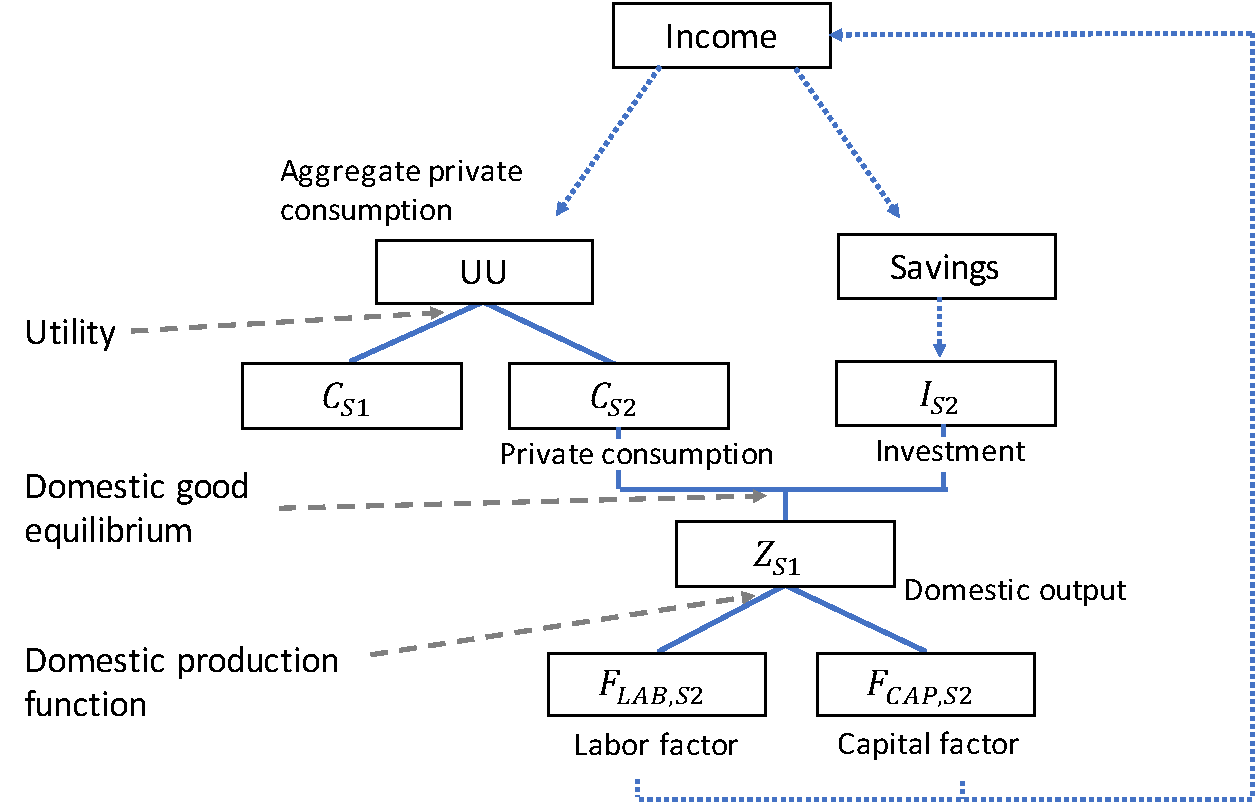
\includegraphics[height=7cm]{figures/overview_closed.pdf}
	\caption{Overview of the closed economy model for the S2 sector}
	\label{fig:overview_closed}
\end{figure}

\subsubsection{Index of sets}
\begin{itemize}
	\item $u$: S1, S2, CAP, LAB, HOH, INV
	\item $i(u)$: S1, S2. Alias: $j(u)$.
	\item $h(u)$: CAP, LAB.
\end{itemize}

\subsubsection{Index of variables}
\begin{itemize}
	
	\item $Z_j$: output of the j-th good
	\item $F_{h,j}$: the h-th factor input by the j-th firm
	\item $FF_h$: the h-th factor supply
	\item $Inc$: Household income
	\item $C_i$: household consumption of the i-th good
	\item $p^x_i$: demand price of the i-th good
	\item $p^z_i$ supply price of the i-th good
	\item $p^f_h$ the h-th factor price
	\item $pc$ consumption price index
	\item $S^p$: private savings	
	\item $U$: unemployment rate
	\item $UU$: utility (Cobb-Douglas)
\end{itemize}

\subsubsection{Index of parameters}
\begin{itemize}
	\item $\alpha_i$: share parameter in utility function
	\item $\sigma^z$: elasticity in CES production function
	\item $\rho^z = \frac{\sigma^z - 1}{\sigma^z}$: param. in CES production function
	\item $\delta_{h,j}$ share parameter in CES production function
	\item $scZ_j$: scale parameter in CES production function  
	\item $\beta_{h,j}$: share parameter in Cobb-Douglas production function
	\item $b_j$: scale parameter in Cobb-Douglas production function
	\item $a_{h,j}$: Leontief coefficient in production function
	\item $\gamma$: wage curve elasticity
	\item $U^0$: initial unemployment rate
\end{itemize}



\subsubsection{Tests}

\paragraph{Walras' law}
Walras' law allows to take off one equation. 
In our numerical application, we remove the market clearing of good for the first sector.
Then, we check after the run that Walras' law is satisfied.

\paragraph{Numéraire}
In our numerical application, we use the price index of consumption goods as the numéraire. 
We check that the model is not sensitive to this assumption. We increase the numéraire by 10\% and rerun the model.
With this assumption, we check that all prices have increased by 10\%, and volumes remain the same.

%%%%%%%%%%%%%%%%%%%%%%%%%%%%%%%%%%%%%%%%%%%%%%%%%%%%%%%%%%%%%%%%%%%%%%%%%%%%%%%%%%%%%%

\clearpage

\subsection{Simple CGE with two labor skills}
\label{app:two_labour_model}

\subsubsection{Overview of the simple CGE with two labor skills}
\begin{figure}[!h]
	\centering
	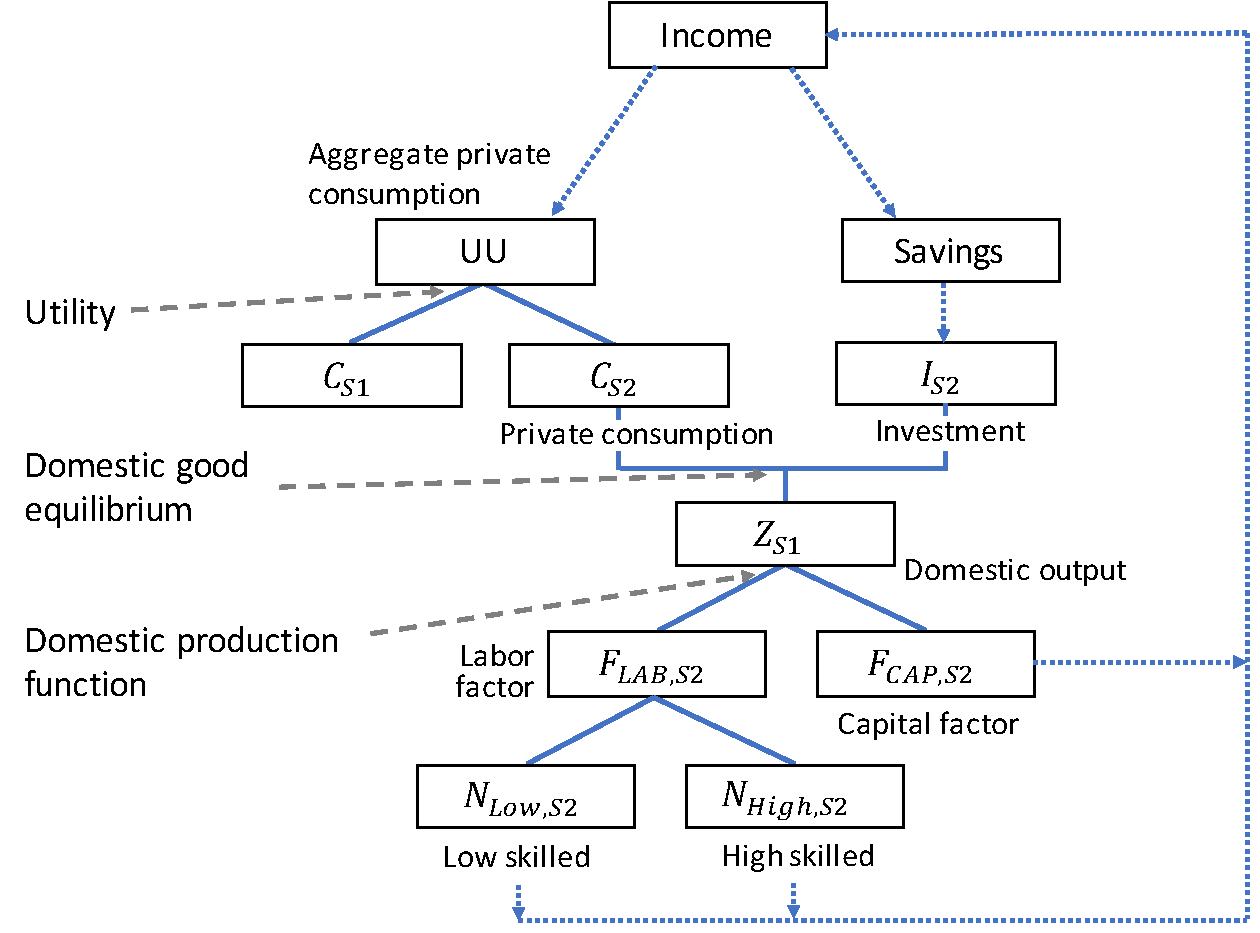
\includegraphics[height=8cm]{figures/overview_twoLabors.pdf}
	\caption{Overview of the open economy model for the S2 sector}
	\label{fig:overview_twoLabors}
\end{figure}

\subsubsection{Index of sets}
\begin{itemize}
	\item $u$: S1, S2, CAP, LAB, HOH, INV
	\item $i(u)$: S1, S2. Alias: $j(u)$
	\item $h(u)$: CAP, LAB
	\item $s$: LABL, LABH 
\end{itemize}


%%%%%%%%%%%%%%%%%%%%%%%%%%%%%%%%%%%%%%%%%%%%%%%%%%%%%%%%%%%%%%%%%%%%%%%%%%%%%%%%%%%%%%



\clearpage

\subsection{Open economy}
\label{app:open_economy_model}

\subsubsection{Overview of the open economy}
\begin{figure}[!h]
	\centering
	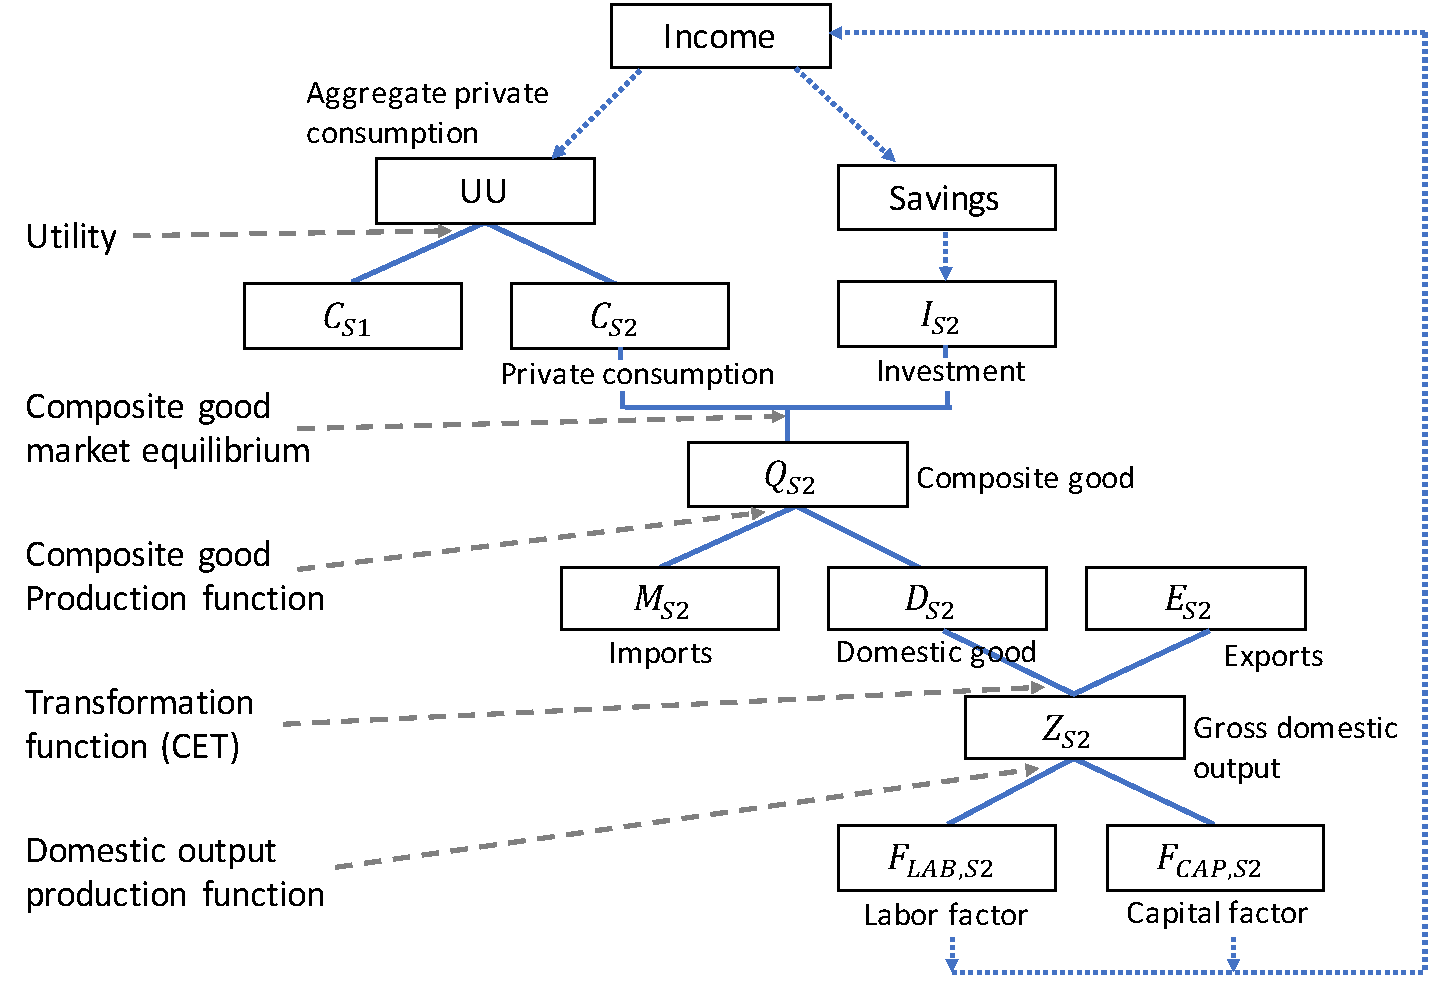
\includegraphics[height=8cm]{figures/overview_open.pdf}
	\caption{Overview of the open economy model for the S2 sector}
	\label{fig:overview_open}
\end{figure}

\subsubsection{Index of sets}
\begin{itemize}
	\item $u$: S1, S2, CAP, LAB, HOH, INV, EXT
	\item $i(u)$: S1, S2
	\item $h(u)$: CAP, LAB
\end{itemize}

\subsubsection{Index of variables}
\begin{itemize}
	\item $Z_j$: output of the j-th good
	\item $FF_h$: factor supply
	\item $F_{h,j}$: the h-th factor input by the j-th firm
	\item $Inc$: Household income
	\item $C_i$: household consumption of the i-th good
	\item $E_i$:  exports
	\item $M_i$:  imports
	\item $Q_i$:  Armingtons composite good
	\item $D_i$:  domestic good

	\item $pf_h$: the h-th factor price
	\item $p^x_i$: consumption price
	\item $p^z_j$: supply price of the i-th good
	\item $p^q_i$: Armingtons composite good price
	\item $p^e_i$: export price in local currency
	\item $p^m_i$: import price in local currency
	\item $p^d_i$: the i-th domestic good price
	\item $\epsilon$: exchange rate
	\item $p^c$: price index

	\item $S^p$: private savings
	\item $S^f$: foreign savings
	\item $U$: unemployment rate
	\item $UU$: utility (Cobb-Douglas)
\end{itemize}

\subsubsection{Index of parameters}
\begin{itemize}
	\item $\alpha^u_i$: share parameter in utility func.
	\item $\sigma^z$: elasticity in CES production function
	\item $\rho^z = \frac{\sigma^z - 1}{\sigma^z}$: param. in CES production function
	\item $\delta_{h,j}$ share parameter in CES production function
	\item $scZ_j$: scale parameter in CES production function  
	\item $\sigma^q$: elasticity of Armington substitution
	\item $\rho^q = \frac{\sigma^q-1}{\sigma^q}$: substitution elasticity parameter for Armington
	\item $\alpha^m_i$: share par. in Armington func.
	\item $\alpha^d_i$: share par. in Armington func.
	\item $scq_i$: scale par. in Armington func.
	\item $\gamma$: wage curve elasticity
	\item $U^0$: initial unemployment rate
\end{itemize}


\subsubsection{Results for IO anc CGE}
\label{subsec:open_economy_results}

\begin{table}[!h]
	\centering
	\caption{SAM results in an open economy with our IO model}
	\label{tab:SAM_IO_openEconomy}
	\begin{tabular}{llllllll}
		\toprule
		& S1 & S2 &  HOH & INV & EXT \\
		\midrule
		S1 &  &   & 8 & 5 & 3 \\
		S2 &  &    & 12 & 3 & 3 \\
		LAB & 9.60 & 8.53 &   &  &  \\
		CAP & 5.33 & 4.74 &   &  &  \\
		EXT & 1.06 & 4.74 &   &  &  \\
		\bottomrule
	\end{tabular}
\end{table}


\begin{table}[!h]
	\centering
	\caption{Open economy with fixed exchange rate $\epsilon$ and endogenous imports}
	\label{tab:SAM_IO_OpenEconomy_noBudget}
	\begin{tabular}{llllll}
		\toprule
		& S1 & S2 & HOH & INV & EXT \\
		\midrule
		S1 &  &  & 10.96 & 5.00 & 0.00 \\
		S2 &  &  & 16.44 & 3.00 & 0.00 \\
		LAB & 9.41 & 8.59 &  &  &  \\
		CAP & 5.23 & 4.77 &  &  &  \\
		EXT & 1.33 & 6.08 &  &  &  \\
		\bottomrule
	\end{tabular}
\end{table}


%%%%%%%%%%%%%%%%%%%%%%%%%%%%%%%%%%%%%%%%%%%%%%%%%%%%%%%%

\clearpage

\subsection{Full model}
\label{sec:full_model}

\subsubsection{Data}
\label{app:full_model_data}

At the 64-sector level of disaggregation, we encounter some issues to calibrate the CGE model:
\begin{itemize}
	\item Postal services (CPA\_H53) have negative capital revenues in 2013. Standard production functions with constant elasticity of substitution cannot account for a negative capital revenue. 
	Since this sector is not crucial for our analysis of green jobs, we aggregate it with the other transportation service (CPA\_H50, CPA\_H51 and CPA\_H52).
	\item The "Manufacture of textiles, wearing apparel and leather products" sector (CPA\_C13-15) and "Computer, electronic and optical products" sector (CPA\_C26) export more than they produce. To avoid issues with negative values in the calibration of trade within the constant elasticity of transformation (CET) function, we aggregate the textile and leather products with "Manufacture of wood and of products of wood" (CPA\_C16) and computers with electrical equipment (CPA\_C27)
	\item The "imputed rent" sector (CPA\_L68A) indicates a low but positive remuneration for employees, but no employee. This would lead to an infinite salary. We aggregate this sector with the other real estate services (CPA\_L68B)
\end{itemize}



\subsubsection{Overview of the full CGE model}

\begin{figure}[!h]
	\centering
	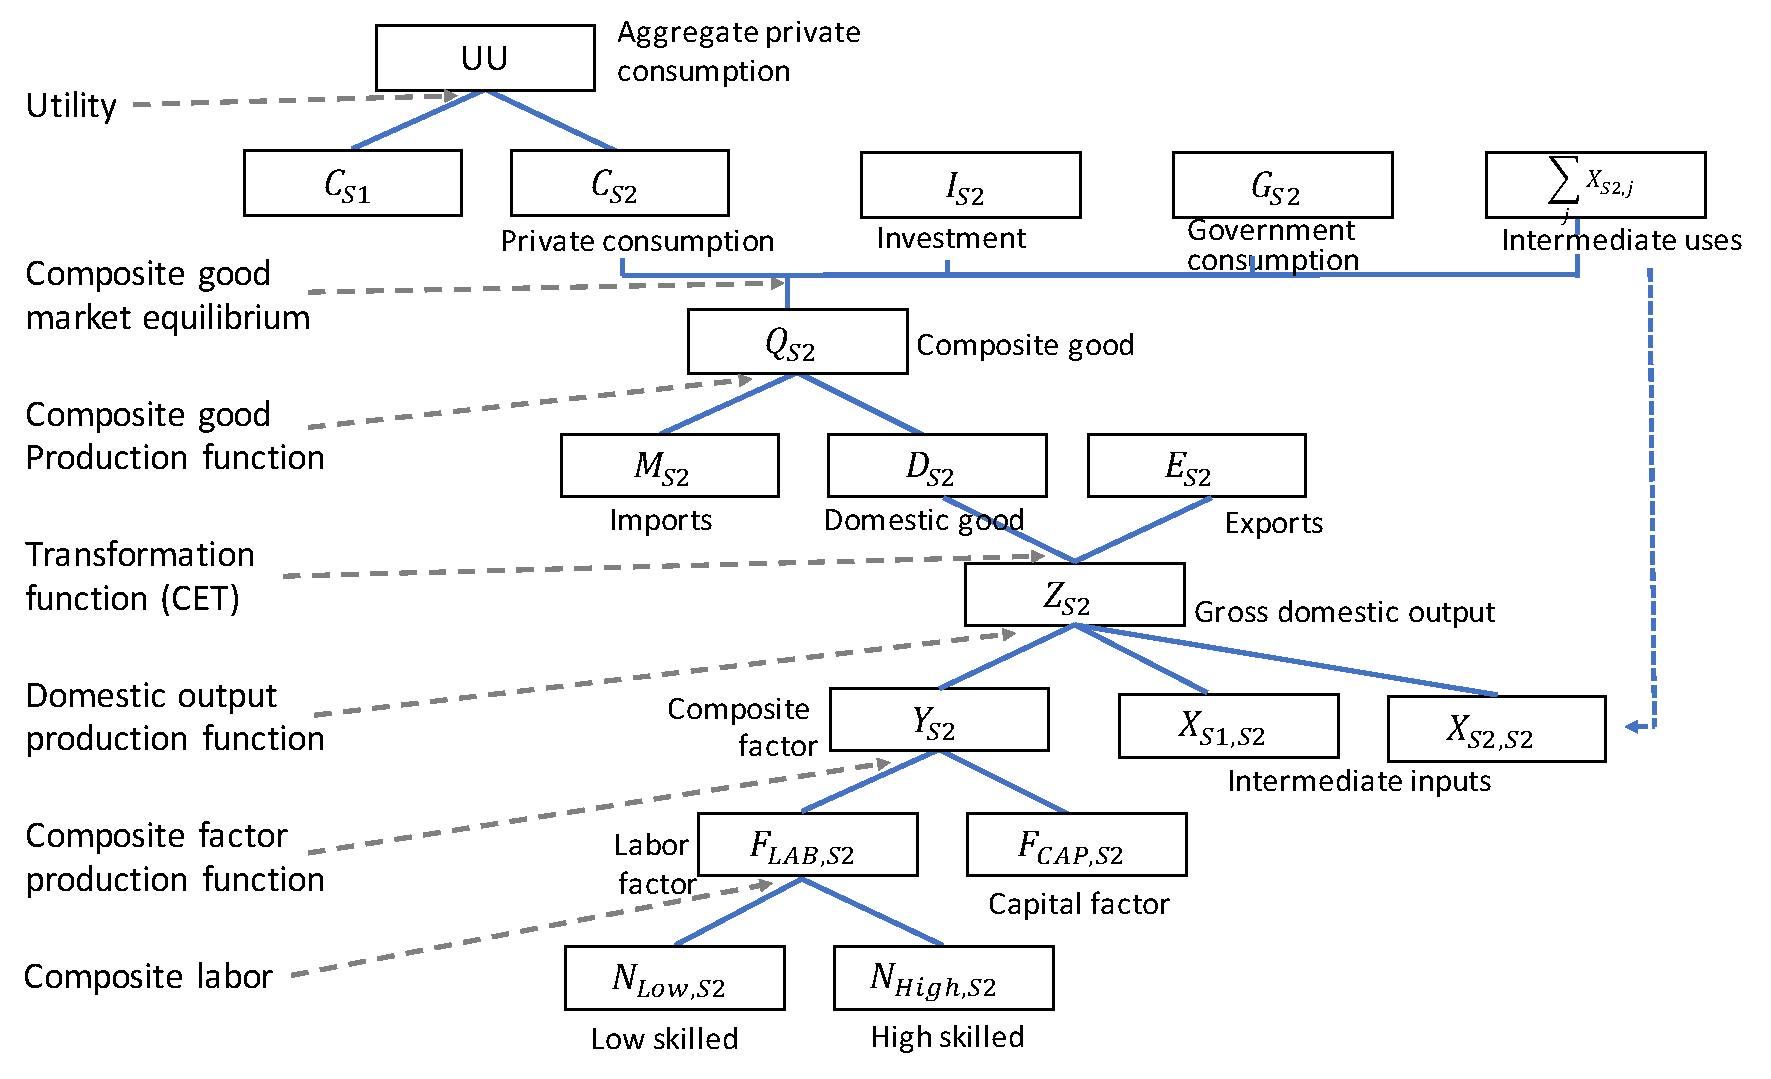
\includegraphics[width=14cm]{figures/overview_full.pdf}
	\caption{Overview of the fully-fledged model for the S2 sector}
	\label{fig:overview_full}
\end{figure}

\subsubsection{Index of sets}
\begin{itemize}
	\item u: SAM entry     /S1*S58, CAP, LAB, IDT, TRF, HOH, GOV,
	\item i(u): goods         /S1*S58/
	\item h(u): factor        /CAP, LAB/
	\item s: labor skill   / highSkill, lowSkill /
\end{itemize}

\subsubsection{Index of variables}
\begin{itemize} 
	\item $Y_j$: composite factor
	\item $Inc$: household income
	\item $N(s,j)$: worker input by skill
	\item $K_j$: capital factor input by the j-th firm
	\item $L_j$: labor input      
	\item $KK$: capital supply
	\item $NN(s)$: worker supply
	\item $X(i,j)$: intermediate input
	\item $Z_j$: output of the j-th good
	\item $C_i$: household consumption of the i-th good
	\item $G_i$: government consumption
	\item $I_i$: investment
	\item $E_i$: exports
	\item $M_i$: imports
	\item $Q_i$: Armington composite good
	\item $D_i$: domestic good

	\item $p^k$: capital factor price
	\item $p^l_j$: labor price
	\item $p^n_s$: workers price
	\item $p^y_j$: composite factor price
	\item $p^z_j$: supply price of the i-th good
	\item $p^q_i$: Armingtons composite good price
	\item $p^e_i$: export price in local currency
	\item $p^m_i$: import price in local currency
	\item $p^d_i$: the i-th domestic good price
	\item $\epsilon$: exchange rate

	\item $S^p$: private saving
	\item $S^g$: government saving
	\item $S^f$: foreign saving
	\item $T^d$: direct tax
	\item $T^z_j$: production tax
	\item $T^p$: private consumption tax
	\item $T^v$: investment tax

	\item $KK$: capital supply
	\item $NN_s$: labor supply
	\item $pc$: consumption price

	\item $UU$: utility (Cobb-Douglas)
\end{itemize}

\subsubsection{Index of parameters}
\begin{itemize}
	\item $\sigma^Y$: elasticity of substitution in composite factor production
	\item $\rho^Y = \frac{\sigma^Y - 1}{\sigma^Y}$: substitution elasticity parameter for capital-labor composite
	\item $\sigma_i$: elasticity of Armington substitution
	\item $\eta_i = \frac{\sigma^z - 1}{\sigma^z}$: substitution elasticity parameter for Armington
	\item $\psi_i$: elasticity of transformation
	\item $\phi_i= \frac{\psi^z - 1}{\psi^z}$: transformation elasticity parameter
	\item $\alpha_i$: share parameter in utility func.
	\item $\delta^l_j$: labor share   in CES prod. func.
	\item $\delta^k_j$: capital share in CES prod. func.
	\item $scY$: scale param.  in CES prod. func.
	\item $\beta\_N(s,j)$: share parameter in labor function
	\item $scL_j$: scale parameter in labor function
	\item $ax(i,j)$: intermediate input requirement coeff.
	\item $ay_j$:  composite fact. input req. coeff.
	\item $\mu_i$:  government consumption share
	\item $\lambda_i$: investment demand share
	\item $\delta^m_i$: share par. in Armington func.
	\item $\delta^d_i$: share par. in Armington func.
	\item $scQ_i$: scale par. in Armington func.
	\item $\xi^d_i$: share par. in transformation func.
	\item $\xi^e_i$: share par. in transformation func.
	\item $\theta_i$: scale par. in transformation func.
	\item $ssg$: average propensity for gov. saving
	\item $\tau^d$: direct tax rate
	\item $Pop$: population (labor force)
	\item $U^0_s$: initial unemployment
	\item $p^{We}_i$: export price in US dollars
	\item $p^{Wm}_i$: import price in US dollars
	\item $\tau^z_i$: production tax rate
	\item $\tau^p$: private consumption tax rate
	\item $\tau^v$: investment tax
	\item $Pop$: population (labor force)
	\item $\gamma$: wage curve elasticity
\end{itemize}



\begin{table}[!h]
	\centering
	\caption{Comparative equations of IO and CGE models. Identical equations are not repeated to facilitate reading. The main differences with the closed version shown in table \ref{tab:closedModel} have their equations labeled in bold.}
	\label{tab:fullModel}
	\begin{tabular}{llll}
		\toprule
		Num & Description & Standard CGE  \\
		\midrule
		eq1 & Production function & $Y_j    = scY_j \cdot  ( \delta^k_j \cdot K_j^{\rho_Y} + \delta^l_j \cdot L_j^{\rho_Y} )^(1/\rho_Y)$ \\
		eq2 & Capital demand & $ K_j = (scY_j^{\rho_Y} \cdot  \delta^k_j \cdot  p^y_j / p^k )^{\sigma_Y} \cdot  Y_j $ \\
		eq3 & Labor demand  & $L_j = (scY_j^{\rho_Y} \cdot \delta^l_j \cdot  p^y_j / p^l_j )^{\sigma_Y} \cdot Y_j $ \\	
		eq4 & Demand of intermediate goods & $X_{i,j}  = ax_{i,j} \cdot Z_j$ \\
		eq5 & Demand of composite factor & $Y_j    = ay_j \cdot Z_j$ \\
		eq6 & Condition of zero profit & $p^z_j   = ay_j \cdot p^y_j + \sum_i ax_{i,j} \cdot p^q_i$ \\
		eq7 & Production of labor composite & $L_j    = scL_j \cdot  \prod_s N_{s,j}^{\beta^N_{s,j}}$  \\
		eq8 & Demand of labor by skill & $N_{s,j}  = \beta^N_{s,j} \cdot p^l_j \cdot  L_j / p^n_s$ \\
		eq9 & Unemployment & $ U_s =  1 - NN_s/Pop_s $\\
		eq10 & Labor supply & $\log( p^n_s / p^c ) = - \gamma \cdot  log(\frac{U_s}{U^0_s}) $  \\
		eq11 & Capital supply & $KK = \overline{KK} $  \\
		\midrule
		eq12 & Direct tax on household & $T^d = \tau^d \cdot Inc $\\
		eq13 & Tax on production & $T^z_j = \tau^z_j \cdot p^z_j \cdot Z_j$ \\
		eq14 & Tax on household consumption & $T^p = \tau^p \cdot \sum_j  p^q_j \cdot C_j $ \\
		eq15 & Tax on investment & $T^v = \tau^v \cdot \sum_j p^q_j\cdot I_j $ \\
		eq16 & Government consumption & $G_i = \mu_i ~ ( T^d + \sum_j T^z_j + T^p + T^v - S^g ) / p^q_i$ \\
		\midrule
		eq17 & Private savings & $S^p = \sum_i (1+\tau^v) \cdot p^q_i \cdot I_i - S^g - \epsilon \cdot S^f$ \\
		eq18 & Government savings & $S^g = ssg \cdot  (T^d + \sum_j T^z_j + T^p + T^v)$ \\
		\midrule
		eq19 & Household income &  $Inc = p^k \cdot KK + \sum_s p^n_s \cdot NN_s $ \\
		eq20 & Houshold consumption & $C_i = \alpha_i \cdot  (Inc -S^p - T^d) / ((1+\tau^p) ~ p^q_i) $ \\
		\midrule
		eq21 & Export demand & $p^e_i = \epsilon \cdot pWe_i$ \\
		eq22 & Import supply & $p^m_i =\epsilon \cdot p^{Wm}_i$ \\
		eq23 & Balance of trade & $\sum_i p^{We}_i \cdot E_i +S^f = \sum_i p^{Wm}_i \cdot M_i$ \\
		eq24 & Trade closure & $S^f = \overline{S^f}$  \quad OR \quad $\epsilon = \overline{\epsilon}$  \\
		\midrule
		eq25 & Armington function & $Q_i = scQ_i \cdot (\alpha^m_i M_i^{\rho_Q} + \alpha^d_i D_i^{\rho_Q}  )^{1/\rho_Q} $ \\
		eq26 & Imports demand & $M_i = \left( scQ_i^{\rho_Q} \cdot \alpha_i^m \cdot \frac{p_i^q}{p_i^m} \right)^{\sigma_Q} Q_i$ \\
		eq27& Domestic demand & $D_i = \left( scQ_i^{\rho_Q} \cdot \alpha_i^d \cdot \frac{p_i^q}{p_i^d} \right)^{\sigma_Q} Q_i$ \\
		eq28 & CET function & $Z_i  = \theta_i \cdot  (\xi^e_i \cdot E_i^{\phi_i} + \xi^d_i \cdot D_i^{\phi_i} )^{(1/\phi_i)} $  \\
		eq29 & Demand of E & $  E_i = (\theta_i^{\phi_i} \cdot \xi^e_i\cdot (1+\tau^z_i) ~ p^z_i/p^e_i)^{(1/(1-\phi_i))} ~Z_i $ \\
		eq30 & Demand of D & $ D_i = (\theta_i^{\phi_i} \cdot \xi^d_i \cdot (1+\tau^z_i) ~ p^z_i/p^d_i)^{(1/(1-\phi_i))} ~ Z_i $ \\
		\midrule
		eq31 &  Balance of domestic good & $Q_i = C_i + I_i$ &  \\
		eq32 & Balance of labor & $NN_s = \sum_j N_{s,j}$ &   \\
		eq33 & Balance of capital & $KK  = \sum_j K_j $ &   \\
		eq34 & Price equality & $p^c_i = p^z_i$ & \\ 
		\bottomrule
	\end{tabular}
\end{table}

\clearpage

\subsubsection{Results}

\subsubsection{Cobb-Douglas elasticity vs Empirical estimates}

\begin{table}[!h]
	\centering
	\caption{Comparing job creation using CES vs Cobb-Douglas \\\hspace{\textwidth} (for a wage curve elasticity $\gamma$=0.1, $\sigma_{Armington}$ =2  and $\psi_{CET}$=2)}
	\label{tab:CobbDouglasError}
	\begin{tabular}{lcccc}
		\toprule
		Techno & Elasticité  &  Value & Value & Error (\%) \\
	    & $\sigma_{KL}$ &  with CES & with Cobb-Douglas& Cobb-Douglas vs CES \\
		\midrule 
		Solar & 0.2 &  5858 & 3542 & -40 \\
Solar & 0.3 &5394 & 3542 & -34 \\
Solar & 0.4 & 5003 & 3542 & -29 \\
Solar & 0.5 & 4670 & 3542 & -24 \\
Solar & 0.6 & 4382 & 3542 & -19 \\
Weatherization & 0.2 & 6589 & 4135 & -37 \\
Weatherization & 0.3 & 6097 & 4135 & -32 \\
Weatherization & 0.4 & 5683 & 4135 & -27 \\
Weatherization & 0.5 & 5331 & 4135 & -22 \\
Weatherization & 0.6 & 5026 & 4135 & -18 \\
		\bottomrule
	\end{tabular}
\end{table}

\clearpage

\subsubsection{Trade}

\begin{figure}[!h]
	\centering
	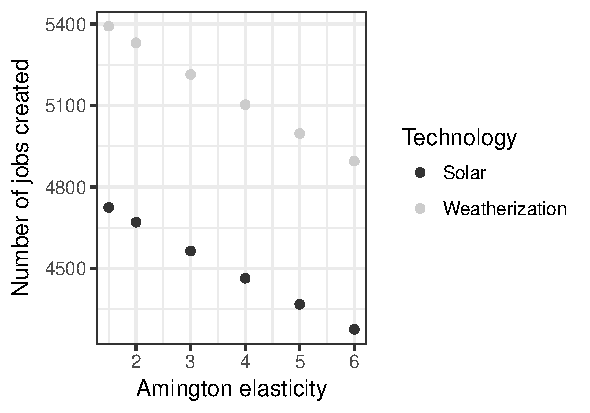
\includegraphics[height=4cm]{figures/Armington.pdf}
	\caption{Impact of the Armington elasticity (with CET elasticity equal to two)}
	\label{fig:armington}
\end{figure}

\begin{figure}[!h]
	\centering
	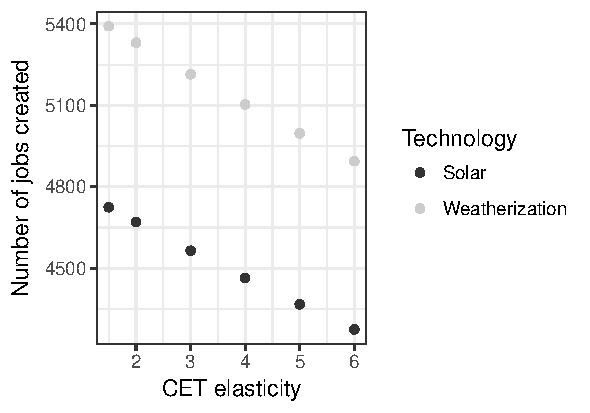
\includegraphics[height=4cm]{figures/CET.pdf}
	\caption{Impact of the CET elasticity (with Armington elasticity equal to two)}
	\label{fig:cet}
\end{figure}

\begin{figure}[!h]
	\centering
	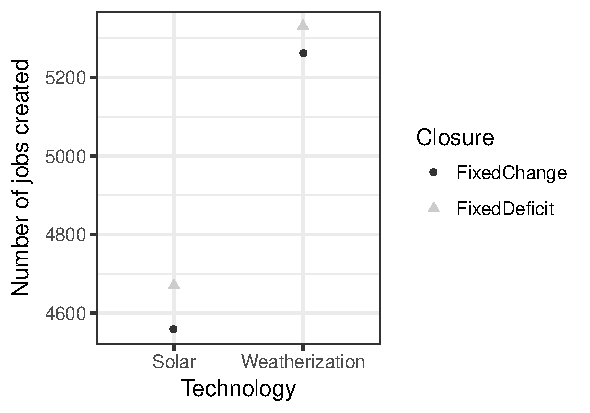
\includegraphics[height=4cm]{figures/closure.pdf}
	\caption{Impact of the trade closure rule}
	\label{fig:closure}
\end{figure}

\subsubsection{Full sensitivity analysis}
\label{sec:full_sensitivity}

\begin{table}
	\small
	\centering
	\caption{Full sensitivity analysis for solar}
	\begin{tabular}{llllllll}
		\toprule
		Techno & gamma & sigma KL & Sigma Armington & Psi CET & CGE Value & IO Value & Ratio \\
		\midrule
		Solar & 0.1 & 0.2 & 1.5 & 1.5 & 6035 & 5010 & 0.83 \\
		Solar & 0.1 & 0.2 & 1.5 & 2 & 5945 & 5010 & 0.84 \\
		Solar & 0.1 & 0.2 & 1.5 & 4 & 5612 & 5010 & 0.89 \\
		Solar & 0.1 & 0.2 & 1.5 & 6 & 5314 & 5010 & 0.94 \\
		Solar & 0.1 & 0.2 & 2 & 1.5 & 5945 & 5010 & 0.84 \\
		Solar & 0.1 & 0.2 & 2 & 2 & 5858 & 5010 & 0.86 \\
		Solar & 0.1 & 0.2 & 2 & 4 & 5534 & 5010 & 0.91 \\
		Solar & 0.1 & 0.2 & 2 & 6 & 5244 & 5010 & 0.96 \\
		Solar & 0.1 & 0.2 & 4 & 1.5 & 5613 & 5010 & 0.89 \\
		Solar & 0.1 & 0.2 & 4 & 2 & 5535 & 5010 & 0.91 \\
		Solar & 0.1 & 0.2 & 4 & 4 & 5245 & 5010 & 0.96 \\
		Solar & 0.1 & 0.2 & 4 & 6 & 4984 & 5010 & 1.01 \\
		Solar & 0.1 & 0.2 & 6 & 1.5 & 5316 & 5010 & 0.94 \\
		Solar & 0.1 & 0.2 & 6 & 2 & 5247 & 5010 & 0.95 \\
		Solar & 0.1 & 0.2 & 6 & 4 & 4985 & 5010 & 1.00 \\
		Solar & 0.1 & 0.2 & 6 & 6 & 4748 & 5010 & 1.06 \\
		Solar & 0.1 & 0.4 & 1.5 & 1.5 & 5130 & 5010 & 0.98 \\
		Solar & 0.1 & 0.4 & 1.5 & 2 & 5066 & 5010 & 0.99 \\
		Solar & 0.1 & 0.4 & 1.5 & 4 & 4823 & 5010 & 1.04 \\
		Solar & 0.1 & 0.4 & 1.5 & 6 & 4603 & 5010 & 1.09 \\
		Solar & 0.1 & 0.4 & 2 & 1.5 & 5066 & 5010 & 0.99 \\
		Solar & 0.1 & 0.4 & 2 & 2 & 5003 & 5010 & 1.00 \\
		Solar & 0.1 & 0.4 & 2 & 4 & 4766 & 5010 & 1.05 \\
		Solar & 0.1 & 0.4 & 2 & 6 & 4551 & 5010 & 1.10 \\
		Solar & 0.1 & 0.4 & 4 & 1.5 & 4824 & 5010 & 1.04 \\
		Solar & 0.1 & 0.4 & 4 & 2 & 4767 & 5010 & 1.05 \\
		Solar & 0.1 & 0.4 & 4 & 4 & 4552 & 5010 & 1.10 \\
		Solar & 0.1 & 0.4 & 4 & 6 & 4355 & 5010 & 1.15 \\
		Solar & 0.1 & 0.4 & 6 & 1.5 & 4605 & 5010 & 1.09 \\
		Solar & 0.1 & 0.4 & 6 & 2 & 4553 & 5010 & 1.10 \\
		Solar & 0.1 & 0.4 & 6 & 4 & 4356 & 5010 & 1.15 \\
		Solar & 0.1 & 0.4 & 6 & 6 & 4175 & 5010 & 1.20 \\
		Solar & 0.1 & 0.6 & 1.5 & 1.5 & 4480 & 5010 & 1.12 \\
		Solar & 0.1 & 0.6 & 1.5 & 2 & 4430 & 5010 & 1.13 \\
		Solar & 0.1 & 0.6 & 1.5 & 4 & 4244 & 5010 & 1.18 \\
		Solar & 0.1 & 0.6 & 1.5 & 6 & 4073 & 5010 & 1.23 \\
		Solar & 0.1 & 0.6 & 2 & 1.5 & 4431 & 5010 & 1.13 \\
		Solar & 0.1 & 0.6 & 2 & 2 & 4382 & 5010 & 1.14 \\
		Solar & 0.1 & 0.6 & 2 & 4 & 4200 & 5010 & 1.19 \\
		Solar & 0.1 & 0.6 & 2 & 6 & 4033 & 5010 & 1.24 \\
		Solar & 0.1 & 0.6 & 4 & 1.5 & 4245 & 5010 & 1.18 \\
		Solar & 0.1 & 0.6 & 4 & 2 & 4201 & 5010 & 1.19 \\
		Solar & 0.1 & 0.6 & 4 & 4 & 4034 & 5010 & 1.24 \\
		Solar & 0.1 & 0.6 & 4 & 6 & 3879 & 5010 & 1.29 \\
		Solar & 0.1 & 0.6 & 6 & 1.5 & 4075 & 5010 & 1.23 \\
		Solar & 0.1 & 0.6 & 6 & 2 & 4035 & 5010 & 1.24 \\
		Solar & 0.1 & 0.6 & 6 & 4 & 3880 & 5010 & 1.29 \\
		Solar & 0.1 & 0.6 & 6 & 6 & 3737 & 5010 & 1.34 \\
		\bottomrule
		\end{tabular}
\end{table}	

\begin{table}
	\small
		\centering
		\caption{Full sensitivity analysis for weatherization}
		\
		\begin{tabular}{llllllll}
		\toprule
		Techno & gamma & sigma KL & Sigma Armington & Psi CET & CGE Value & IO Value & Ratio \\
		\midrule
		Weatherization & 0.1 & 0.2 & 1.5 & 1.5 & 6782 & 8050 & 1.19 \\
		Weatherization & 0.1 & 0.2 & 1.5 & 2 & 6684 & 8050 & 1.20 \\
		Weatherization & 0.1 & 0.2 & 1.5 & 4 & 6321 & 8050 & 1.27 \\
		Weatherization & 0.1 & 0.2 & 1.5 & 6 & 5997 & 8050 & 1.34 \\
		Weatherization & 0.1 & 0.2 & 2 & 1.5 & 6683 & 8050 & 1.20 \\
		Weatherization & 0.1 & 0.2 & 2 & 2 & 6589 & 8050 & 1.22 \\
		Weatherization & 0.1 & 0.2 & 2 & 4 & 6237 & 8050 & 1.29 \\
		Weatherization & 0.1 & 0.2 & 2 & 6 & 5921 & 8050 & 1.36 \\
		Weatherization & 0.1 & 0.2 & 4 & 1.5 & 6321 & 8050 & 1.27 \\
		Weatherization & 0.1 & 0.2 & 4 & 2 & 6236 & 8050 & 1.29 \\
		Weatherization & 0.1 & 0.2 & 4 & 4 & 5921 & 8050 & 1.36 \\
		Weatherization & 0.1 & 0.2 & 4 & 6 & 5637 & 8050 & 1.43 \\
		Weatherization & 0.1 & 0.2 & 6 & 1.5 & 5998 & 8050 & 1.34 \\
		Weatherization & 0.1 & 0.2 & 6 & 2 & 5922 & 8050 & 1.36 \\
		Weatherization & 0.1 & 0.2 & 6 & 4 & 5638 & 8050 & 1.43 \\
		Weatherization & 0.1 & 0.2 & 6 & 6 & 5380 & 8050 & 1.50 \\
		Weatherization & 0.1 & 0.4 & 1.5 & 1.5 & 5824 & 8050 & 1.38 \\
		Weatherization & 0.1 & 0.4 & 1.5 & 2 & 5753 & 8050 & 1.40 \\
		Weatherization & 0.1 & 0.4 & 1.5 & 4 & 5486 & 8050 & 1.47 \\
		Weatherization & 0.1 & 0.4 & 1.5 & 6 & 5244 & 8050 & 1.54 \\
		Weatherization & 0.1 & 0.4 & 2 & 1.5 & 5753 & 8050 & 1.40 \\
		Weatherization & 0.1 & 0.4 & 2 & 2 & 5683 & 8050 & 1.42 \\
		Weatherization & 0.1 & 0.4 & 2 & 4 & 5423 & 8050 & 1.48 \\
		Weatherization & 0.1 & 0.4 & 2 & 6 & 5187 & 8050 & 1.55 \\
		Weatherization & 0.1 & 0.4 & 4 & 1.5 & 5486 & 8050 & 1.47 \\
		Weatherization & 0.1 & 0.4 & 4 & 2 & 5423 & 8050 & 1.48 \\
		Weatherization & 0.1 & 0.4 & 4 & 4 & 5187 & 8050 & 1.55 \\
		Weatherization & 0.1 & 0.4 & 4 & 6 & 4971 & 8050 & 1.62 \\
		Weatherization & 0.1 & 0.4 & 6 & 1.5 & 5245 & 8050 & 1.53 \\
		Weatherization & 0.1 & 0.4 & 6 & 2 & 5188 & 8050 & 1.55 \\
		Weatherization & 0.1 & 0.4 & 6 & 4 & 4972 & 8050 & 1.62 \\
		Weatherization & 0.1 & 0.4 & 6 & 6 & 4774 & 8050 & 1.69 \\
		Weatherization & 0.1 & 0.6 & 1.5 & 1.5 & 5135 & 8050 & 1.57 \\
		Weatherization & 0.1 & 0.6 & 1.5 & 2 & 5080 & 8050 & 1.58 \\
		Weatherization & 0.1 & 0.6 & 1.5 & 4 & 4873 & 8050 & 1.65 \\
		Weatherization & 0.1 & 0.6 & 1.5 & 6 & 4684 & 8050 & 1.72 \\
		Weatherization & 0.1 & 0.6 & 2 & 1.5 & 5080 & 8050 & 1.58 \\
		Weatherization & 0.1 & 0.6 & 2 & 2 & 5026 & 8050 & 1.60 \\
		Weatherization & 0.1 & 0.6 & 2 & 4 & 4824 & 8050 & 1.67 \\
		Weatherization & 0.1 & 0.6 & 2 & 6 & 4639 & 8050 & 1.74 \\
		Weatherization & 0.1 & 0.6 & 4 & 1.5 & 4873 & 8050 & 1.65 \\
		Weatherization & 0.1 & 0.6 & 4 & 2 & 4824 & 8050 & 1.67 \\
		Weatherization & 0.1 & 0.6 & 4 & 4 & 4639 & 8050 & 1.74 \\
		Weatherization & 0.1 & 0.6 & 4 & 6 & 4468 & 8050 & 1.80 \\
		Weatherization & 0.1 & 0.6 & 6 & 1.5 & 4684 & 8050 & 1.72 \\
		Weatherization & 0.1 & 0.6 & 6 & 2 & 4640 & 8050 & 1.74 \\
		Weatherization & 0.1 & 0.6 & 6 & 4 & 4469 & 8050 & 1.80 \\
		Weatherization & 0.1 & 0.6 & 6 & 6 & 4310 & 8050 & 1.87 \\
		\bottomrule
	\end{tabular}
\end{table}


\end{subappendices}

\newrefsection
\selectlanguage{french}
\chapter{Conclusion} \label{chap:conclusion}

\section{Apports de la thèse}

Dans cette thèse, j’ai cherché à apporter des éléments de compréhension et de réponse sur deux thèmes majeurs autour des énergies renouvelables : le choix d’une stratégie de déploiement à long terme et leurs impacts sur l’emploi. 

La réflexion sur le choix d’une stratégie est menée dans le chapitre \ref{chap:nuclear_bet}. L’originalité de ma recherche consiste à intégrer pleinement les questions d’incertitudes dans la réflexion sur une trajectoire de mix électrique, en m’appuyant sur le cas du secteur électrique français.
Cette nouvelle approche conduit à un renversement significatif par apport aux méthodes traditionnelles consistant à déterminer un unique optimum minimisant les coûts. 
En effet, le concept même d’optimum n’est plus adapté lorsque les incertitudes sont trop importantes : différentes hypothèses également plausibles mènent à différents optima, entre lesquels il est impossible de choisir. Je me suis donc tourné vers la recherche de stratégies robustes, c’est-à-dire satisfaisantes pour un grand nombre de valeurs plausibles des paramètres. Pour y parvenir, je me suis appuyé sur un outil développé et utilisé dans le champ des sciences du climat, que j’ai appliqué de façon originale au mix électrique.
J’ai également cherché à comprendre et expliquer les termes du débat actuel. Je n’apporte donc pas une unique solution « rationnelle », mais je montre au contraire que différentes options sont défendables, selon l’hypothèse portée sur l’évolution de paramètres futurs. Mais mon travail a permis de simplifier les termes du débat. Plutôt que de devoir se prononcer sur les multiples sources d’incertitudes, j’ai distingué quelques grandes visions contrastées. Ce travail permet de clarifier et faciliter le pari que doivent faire les dirigeants devant prendre une décision en situation d’incertitude. 
L’application au cas du secteur électrique français a permis de retrouver les scénarios présents lors du débat national sur la transition énergétique. Mais j’ai surtout pu mettre en évidence de nouvelles trajectoires. Mon analyse montre que la prolongation de tous les réacteurs est loin d’être une évidence. La baisse des coûts du renouvelables, l’incertitude sur la demande, le prix du CO2 et le coût de rénovation des centrales nucléaires existantes plaident pour une stratégie plus diversifiée.
Une rénovation complète court le risque de voir les réacteurs nucléaires fonctionner en semi-base ou pointe, en cas de baisse de la demande d’électricité. Elle rend en outre extrêmement vulnérable à un coût de rénovation des centrales plus élevé que prévu, voire à un défaut générique. 
D’après mes résultats, des stratégies robustes impliquent de fermer 7 à 14 réacteurs. Cette proposition se démarque des deux positions les plus visibles dans le débat français, la rénovation complète et la sortie complète. Ces deux extrêmes sont souvent défendus sur la base d’une vision binaire comparant les coûts des technologies. Elles font ainsi l’impasse sur le problème des coûts d’intégration des renouvelables – ou, pour le dire autrement, de leur valeur marginale pour le système -, et sur les questions d’incertitudes. 
Prendre ces incertitudes à bras-le-corps, et les étudier avec un modèle tenant compte des coûts d’intégration abouti m’a donc permis de découvrir de nouvelles options plus robustes pour une stratégie française de déploiement des renouvelables.



Les chapitres \ref{chap:TE_Emploi} et \ref{chap:mechanisms} sont centrés sur le deuxième aspect de ma thèse : la question de l’emploi dans la transition énergétique.

Le chapitre \ref{chap:TE_Emploi} a permis de clarifier la notion de contenu en emploi.  Je commence par proposer une métrique pour ce terme. En effet, plusieurs définitions apparaissent dans la littérature, mais conduisent à des biais pour estimer les emplois nets. Je retiens la définition d’un nombre d’ETP par unité monétaire de demande finale.
Ensuite, j’ai mesuré ce contenu en emploi pour différentes branches de l’économie. En croisant ce contenu en emploi avec le contenu en émissions, je mets ainsi en évidence quelques secteurs faiblement émetteurs et fortement créateurs d’emplois. Réorienter l’investissement vers ces secteurs satisfait donc au double impératif d’une transition écologique et sociale – sous réserve de rester dans les limites de validité du modèle input-output utilisé.

Mais la vraie originalité de ce chapitre a été de décomposer le contenu en emploi des différentes branches, pour faire apparaître quatre facteurs : le taux d’importations finales, le taux d’importations intermédiaires, le niveau de taxes et de subventions, la part des salaires dans la valeur ajoutée, et enfin le niveau des salaires.
Cette décomposition permet d’améliorer la compréhension de ce qu’est le contenu en emploi. En l’appliquant, il est possible de déterminer si le contenu en emploi d’une branche est élevé grâce à ses faibles importations, une part importante du travail dans la valeur ajoutée, de faibles taxes, ou à cause de bas salaires.
Cette nouvelle information a notamment révélé un biais du contenu en emploi, relatif à l’impact des taxes et subventions. Les secteurs fortement subventionnés -- notamment celui de l'agriculture en France -- présentent un fort contenu en emploi. Mais ces subventions devront être financées par des prélèvements ailleurs dans l’économie, avec un impact négatif qui n’est pas pris en compte dans le contenu en emploi. Notre décomposition permet de mesurer ce biais, et donc de le corriger. 
En outre, notre méthodologie de décomposition peut être appliquée de façon prospective, pour décomposer les créations d’emplois liées à la réallocation de la demande finale d’un secteur vers un autre (avec toutes les précautions nécessaires liées à l’utilisation des modèles IO). Ces informations peuvent être utile à l’économiste et au décideur : l’impact économique, social et politique est en effet différent si les nouveaux emplois proviennent d’une réduction des importations ou de salaires plus faibles. Dans un cas, il s’agit de relocaliser la production, au détriment d’autres pays, donc d’une redistribution internationale des richesses ; dans l’autre, de partager les revenus du travail, avec des conséquences redistributives nationales.
Cette décomposition permet de mieux comprendre les mécanismes à l’œuvre dans les modèles macro-économiques. Encourager un secteur intensif en main-d’œuvre plutôt qu’en capital va augmenter la demande de travail ; réduire les importations va augmenter la valeur ajoutée locale ; baisser les salaires peut avoir un impact négatif sur le pouvoir d’achat. L’idée n’est bien sûr pas de se substituer aux modèles macro-économiques, mais bien d’apporter un éclairage sur les mécanismes économiques qu’ils mettent en jeu.



Dans le chapitre \ref{chap:mechanisms}, j’ai poursuivi cette réflexion sur les mécanismes économiques présidant à de la création d’emploi. J’étudie plus spécifiquement les impacts d’une réallocation des investissements vers des secteurs bas carbone, comme l’isolation des bâtiments ou le déploiement de panneaux solaires.  Cette réallocation est en effet nécessaire pour décarboner l’économie et atteindre nos objectifs climatiques. 
Dans cette partie, je m’attache à déterminer les mécanismes économiques sous-jacents à l’impact sur l’emploi. Dans la continuité du chapitre précédent, je mets en évidence et j’étudie trois phénomènes : l’impact des importations, de la part des revenus du travail dans la valeur ajoutée, et du niveau des salaires.

Par rapport au chapitre précédent, cette nouvelle partie apporte plusieurs précisions quant à la logique économique et la robustesse des résultats sur la création d’emplois. 
Je montre qu’il est possible de créer de l’emploi en favorisant des secteurs avec une plus grande part des revenus dans la valeur ajoutée ou des salaires plus faibles. En revanche, mes résultats jettent un doute sur le bénéfice d’encourager les secteurs pour leur caractère local et non-délocalisable. En équilibre général, la réduction des importations mène en effet à des rétroactions qui annulent les bénéfices attendus.
Mes recherches portent également une réflexion sur l’usage et la validité des modèles économiques utilisés pour les études en emploi liés à la transition énergétique. Je montre ainsi que les modèles input-output, souvent utilisés, donnent des valeurs de créations d’emplois près de deux fois plus élevées que les modèles d’équilibre général. Les modèles IO tendent en effet à surestimer l’impact d’une forte part des salaires dans la valeur ajoutée, et voient un effet très positif d’une réduction des importations – à l’opposé des modèles d’équilibre général dans lesquels cet effet est nul.
Mais je montre également que de nombreux modèles CGE sous-estiment l’impact sur l’emploi. Ils utilisent des fonctions Cobb-Douglas très pratiques d’un point de vue calculatoire, mais font ainsi l’hypothèse d’une élasticité capital-travail unitaire. Or, des études empiriques montrent que cette élasticité est significativement inférieure à 1, et varie plutôt de 0.2 à 0.6 \citep{VanderWerf2008}. Dans mes scénarios, cette mauvaise valeur de l’élasticité réduit les effets positifs sur l’emploi de 20 à 40 \% par rapport aux résultats avec des valeurs empiriques. 

Au final, mes résultats indiquent qu’il est possible de créer des emplois en investissant dans des secteurs intensifs en travail plutôt qu’en capital, et où les salaires sont plus faibles. L’environnement et l’écologie peuvent aller de pair. Il s’agit d’un message fort pour accélérer la transition énergétique.
Mais mon analyse appelle également à utiliser avec prudence les annonces quantifiées en termes d’emplois : les modèles IO auront tendance à être optimistes, et de nombreux modèles CGE seront au contraire pessimistes.
Enfin, mon travail remet en cause l’argument souvent utilisé du bénéfice à développer des énergies renouvelables locales, qui permettraient ainsi de réduire les importations. Le poids politique de cet argument et son côté intuitif semblent inversement proportionnels à sa robustesse dans les analyses économiques.


\section{Ouverture}

Mes travaux sur la stratégie optimale du parc nucléaire proposent un cadre flexible, qui pourrait être mis à jour régulièrement afin d’intégrer les nouvelles informations en termes de coûts, de demande d’électricité ou de prix du CO2. 

Ce modèle pourrait bien sûr bénéficier de plusieurs améliorations. Pour des raisons de temps de calcul, j’ai en effet dû réaliser des arbitrages de modélisation. Je vois deux grands points d’amélioration. Le premier a trait aux impacts des variations imprévues de la production renouvelable. La représentation des erreurs de prédiction intra-horaire n’a pas été modélisée. Ces erreurs de prédiction ont fortement diminué depuis quelques années. En Espagne, l’erreur à 1h a été divisé par trois en cinq ans, passant de 12 \% à 4 \% \citep{IRENA2017}, mais les progrès ont cessé depuis. Il serait intéressant de regarder plus avant cette question, afin de s’assurer que les résultats ne sont pas affectés. Le volet demande d’électricité pourrait également être affiné. L’importance des politiques de demande en complément de la politique d’offre a été soulignée à de nombreuses reprises par l’IDDRI \citep{Berghmans2017}. Une modélisation plus avancée des secteurs, et de leur capacité à réduire et déplacer leur consommation actuelle ou à venir, apporterait un réalisme et une précision accrus. Ce volet demande pourrait s'inspirer des travaux réalisés par \citet{RTE2016} dans son \textit{Bilan Prévisionnel 2016} ou encore par ceux de l'\citet{ADEME2015} dans son analyse d'un mix 100 \% renouvelable.

Mais le plus intéressant est peut-être à chercher du côté des nouvelles technologies émergentes. 
Les éoliennes offshores semblent être à l’aube d’une expansion rapide. Fin 2016, la capacité cumulée atteignait 12,6 GW. Et cette capacité pourrait doubler d’ici 2020. Ce boom est accompagné d’une chute rapide des prix. Un rapport de McKinsey publié en mai 2017 s’intitule d’ailleurs « Winds of change? Why offshore wind might be the next big thing » \citep{McKinsey2017Wind}. En novembre 2016, un appel d’offre au Danemark s’est conclu au prix de 49.9 euros par MWh. Un record absolu pour cette technologie, qui se rapproche rapidement de la compétitivité avec les autres sources d’électricité (pour comparaison, le tarif d'achat du nucléaire historique en France est de 42 euros/MWh, et celui des éoliennes de 82 euros/MWh). Les éoliennes offshores sont intéressantes à double titre : leur installation rencontre moins d’oppositions locales que les éoliennes terrestres, et leur production est plus stable, ce qui augmente la valeur de leur production pour le système électrique \citep{Hirth2016}.

Le power-to-gas est également une source d’énergie qui pourrait s’avérer importante pour l’avenir. Elle permet de bénéficier du faible coût variable des renouvelables, et participer à gérer les surplus de production. Son intérêt s’étend même au-delà du seul secteur électrique, avec la possibilité de fabriquer du gaz ensuite réinjecté sur le réseau, et utilisé directement par les secteurs industriels ou tertiaires. Cette technologie crée donc un pont entre les secteurs électriques et gaziers, dont il serait intéressant d’explorer les conséquences. En janvier 2016, plus de 50 projets pilotes étaient lancés à travers le monde \citep{EneaConsulting2016}. Et cette technique est l’une des clés de voute du scénario négaWatt, ce qui souligne le rôle important que peut avoir cette technologie pour une politique ambitieuse de réduction des émissions.


Du côté de l’emploi, j’aurais voulu poursuivre mon analyse en m’intéressant aux effets transitoires et au rôle de la monnaie, par exemple en mobilisant des modèles de type nouveau-keynésien, comme dans \citet{Blanchard2007}. 
Plus fondamentalement, mes questionnements ont porté sur la pertinence et l’importance des choix de modélisations sur les résultats. Cela s’est traduit par la comparaison de modèles dans le chapitre \ref{chap:mechanisms}, et l’analyse de nombreuses spécifications différentes et tests de sensibilité : sur l’ajustement de la balance commerciale, le marché de travail, etc. 
Mais ces interrogations sur les modèles pourraient être étendues à d'autres hypothèses plus fondamentales encore. En particulier le questionnement de l’utilisation d’un agent représentatif, parfaitement rationnel et informé, me paraît un axe de recherche encourageant. Bien sûr, les critiques de cet \textit{homo economicus} ne sont pas nouvelles. Carl Menger critiquait l’hypothèse implicite d’homogénéité des individus ; Keynes l’hypothèse d’information complète ; Veblen la rationalité parfaite ; \citet{Bourdieu1977} l’a qualifié de « monstre anthropologique », et \citet{Sen2012} de « demeuré social » ; plus récemment, les travaux de l’économie comportementale ont mis en évidence de nombreux biais cognitifs \citep{Thaler2009,Kahneman2011}.
Mais l’ampleur des critiques souligne le chemin qui reste à parcourir. Des pistes qui me semblent intéressantes ont trait à la compréhension et la modélisation du comportement des agents. L'hypothèse de «~rationalité parfaite~», malgré son appellation flatteuse, est finalement une représentation très stylisée de la façon dont nous prenons une décision. Il devrait donc être possible d'enrichir cette représentation, de se rapprochant des comportements observés dans les autres sciences sociales. Par exemple, des travaux récents explorent l’impact d’agents « presque parfaitement rationnels » (near-rational expectations). Ainsi, \citet{Farhi2016} montre que l’effet des politiques monétaires est alors plus faible que ce qu’indiquent les modèles à agents rationnels.

Par ailleurs, l’explosion des capacités computationnelles ouvre le champ à l’introduction de modèles avec de nombreux agents représentatifs – plusieurs centaines ou milliers –, ce qui pourrait permettre de dégager des dynamiques agrégées qui échappent à des modèles représentant seulement un ou quelques agents représentatifs. Des travaux récents vont dans cette direction. Ainsi, \citet{Kaplan2016} montre que les effets de la politique monétaires sont très différents dans des modèles à agents représentatifs et dans des modèles à agents hétérogènes. 

Représenter explicitement des agents multiples, dans leur diversité et leur imperfection, me paraît être une piste de recherche intéressante double titre. Elle peut permettre à l’économie de renforcer ses fondements empiriques, de poser ainsi des hypothèses vérifiables et réfutables – critère de scientificité selon Popper – et d’abandonner, le cas échéant, des hypothèses contredites par l’expérience. Englober la théorie du choix rationnel dans un modèle plus global de l’action peut être l’occasion de renouer des liens avec les autres sciences sociales, notamment l’anthropologie, la psychologie et la sociologie. “L'économie qui est la science sociale mathématiquement la plus avancée, est la science socialement la plus arriérée, car elle s'est abstraite des conditions sociales, historiques, politiques, psychologique, écologiques inséparables des activités économiques » constate \citet{Morin1999}. Sortir de ce fonctionnement en silos, se rapprocher des autres disciplines pour mieux appréhender la complexité de l'humain : voilà qui me paraît une piste prometteuse de recherche future.






\phantomsection
\printbibliography[heading=subbibintoc]

\singlespacing 


\selectlanguage{english}
\chapter*{Colophon}

\begin{center}
\parbox{200pt}{\raggedright\lettrine[lines=3,slope=-2pt,nindent=-4pt]{\textcolor{SchoolColor}{T}}{his thesis was typeset} using \LaTeX, originally developed by Leslie Lamport and based on Donald Knuth's \TeX. The body text is set in 11 point Arno Pro, designed by Robert Slimbach in the style of book types from the Aldine Press in Venice, and issued by Adobe in 2007. A template, which can be used to format a PhD thesis with this look and feel, has been released under the permissive \textsc{mit} (\textsc{x}11) license, and can be found online at \href{https://github.com/suchow/}{github.com/suchow/} or from the author at \href{mailto:suchow@fas.harvard.edu}{suchow@post.harvard.edu}.
}
\end{center}

\end{document}
